\subsection{Аналоговая электроника}
	
	\subsubsection{Аннотация}

	Общее впечатление студентов от курса по аналоговой электронике крайне негативное.

	Лекции Дунаевой М.А. получили крайне негативные отзывы. Респонденты отметили, что лекции абсолютно бесполезны для усвоения материалов курса. Совет студентов и аспирантов ФРКТ предлагает заменить лектора на Григорьева А.А., руководствуясь развернутыми отзывами студентов.
	
	Респонденты отметили положительными оценками работу таких преподавателей, как Григорьев И.А., Неешпапа А.В., Зарипов Р.А. Совет студентов и аспирантов ФРКТ предлагает поощрить перечисленных преподавателей.
	
	Студенты недовольны качеством преподаваемых лекций и имеющихся материалов, в результате чего обучающиеся отмечают крайне тяжелую сложность освоения теоретической информации, необходимой для понимания курса. Многие отметили, что оборудование для лабораторных работ устарело и часто не работает, что затрудняет выполнение заданий. Курс считается устаревшим и неактуальным для современных реалий. Студенты отмечают, что полученные знания не пригодятся в будущем.

	Экзамен 30 декабря вызвал недовольство студентов. Совет студентов и аспирантов ФРКТ предлагает проводить экзамен в более ранние сроки. Если не будет свободных поточных аудиторий для сдачи, можно проводить экзамен в аудиториях Радиотехнического корпуса -- по аналогии с экзаменом на кафедре теоретической механики.

	Руководствуясь результатами опроса, Совет студентов и аспирантов ФРКТ выдвигает следующие идеи по улучшению данного курса:
	\begin{enumerate}
		\item полный пересмотр учебной программы курса;
		\item пересмотр формата курса / введение альтернативного курса проектных лабораторных работ, аналогичных тем, которые есть на кафедре общей физики, для последующей полноценной интеграции в образовательную программу кафедры;
		\item пересмотр кандидатуры лектора;
		\item разбор теоретических задач на занятиях по лабораторным работам;
		\item обновление оборудования.
	\end{enumerate}

	Учебный департамент Совета студентов и аспирантов ФРКТ готов оказать любую помощь в улучшении программы курса.

	\subsubsection{Общий отзыв студентов о курсе}

		\begin{figure}[H]
			\centering
			\begin{subfigure}[b]{0.45\textwidth}
				\centering
				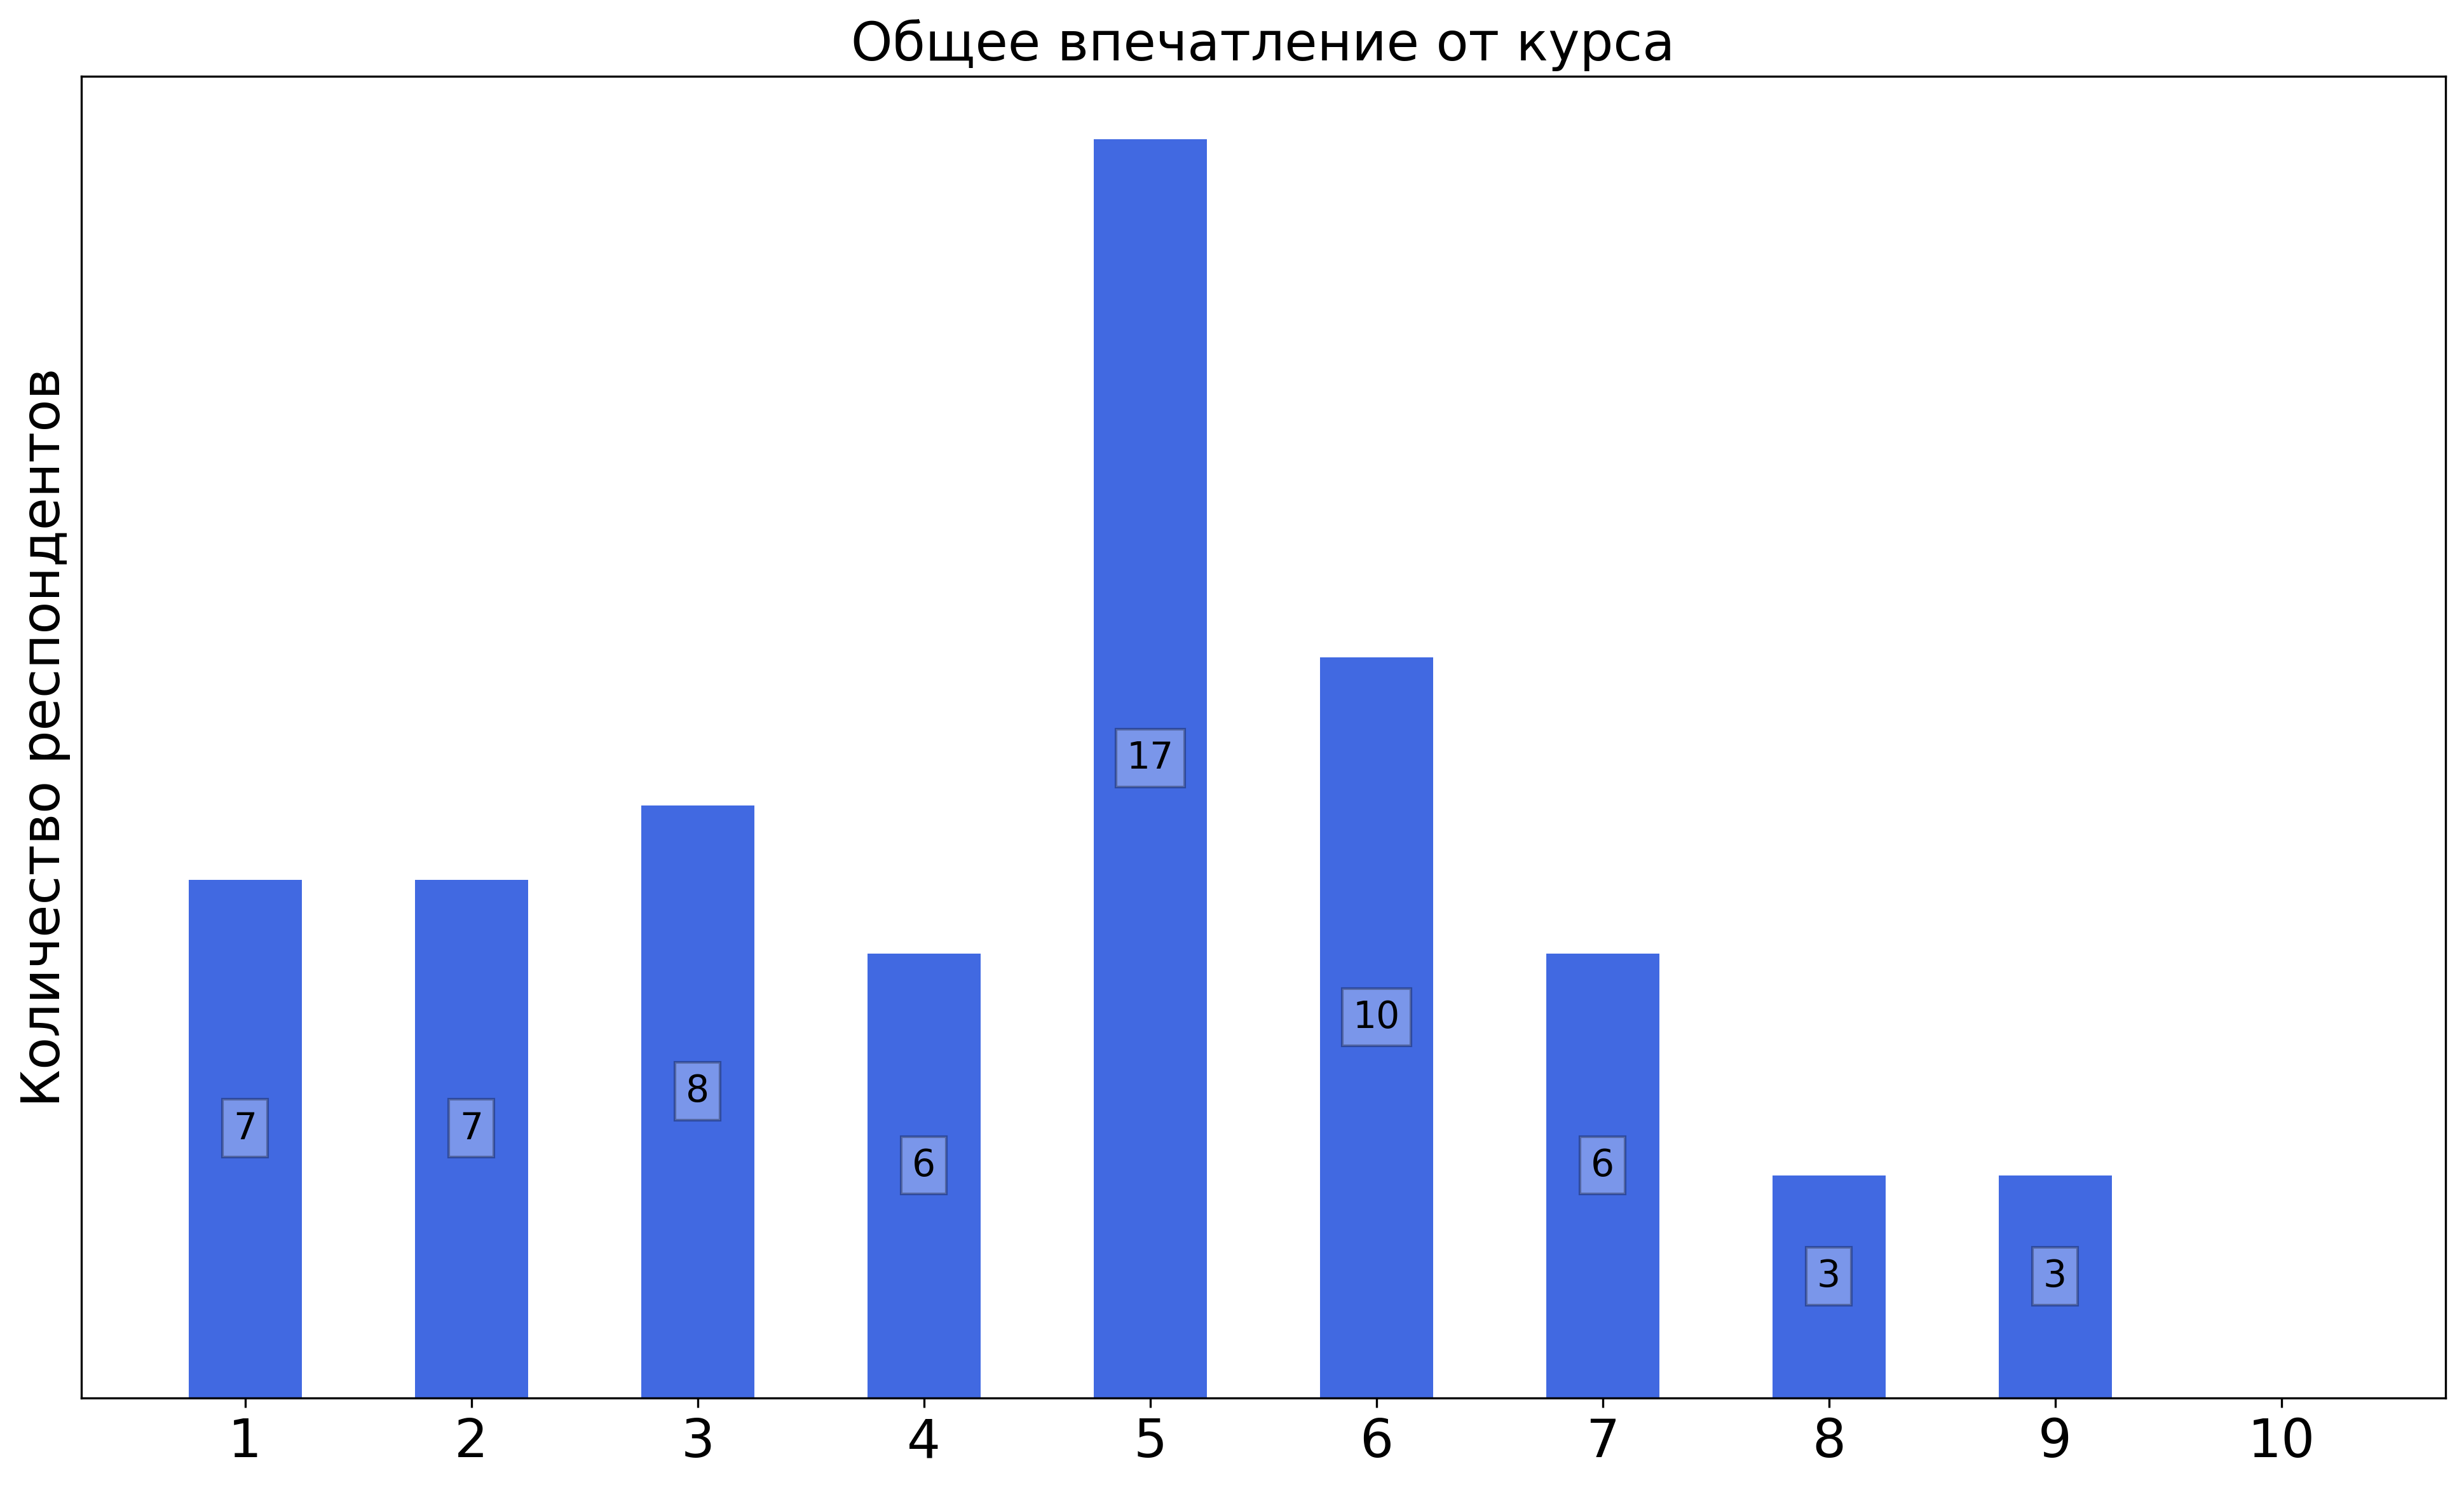
\includegraphics[width=\textwidth]{images/3 course/Аналоговая электроника/general-0.png}
			\end{subfigure}
		\end{figure}

	\subsubsection{Материалы, использумые респондентами при изучении курса}

		\begin{figure}[H]
			\centering
			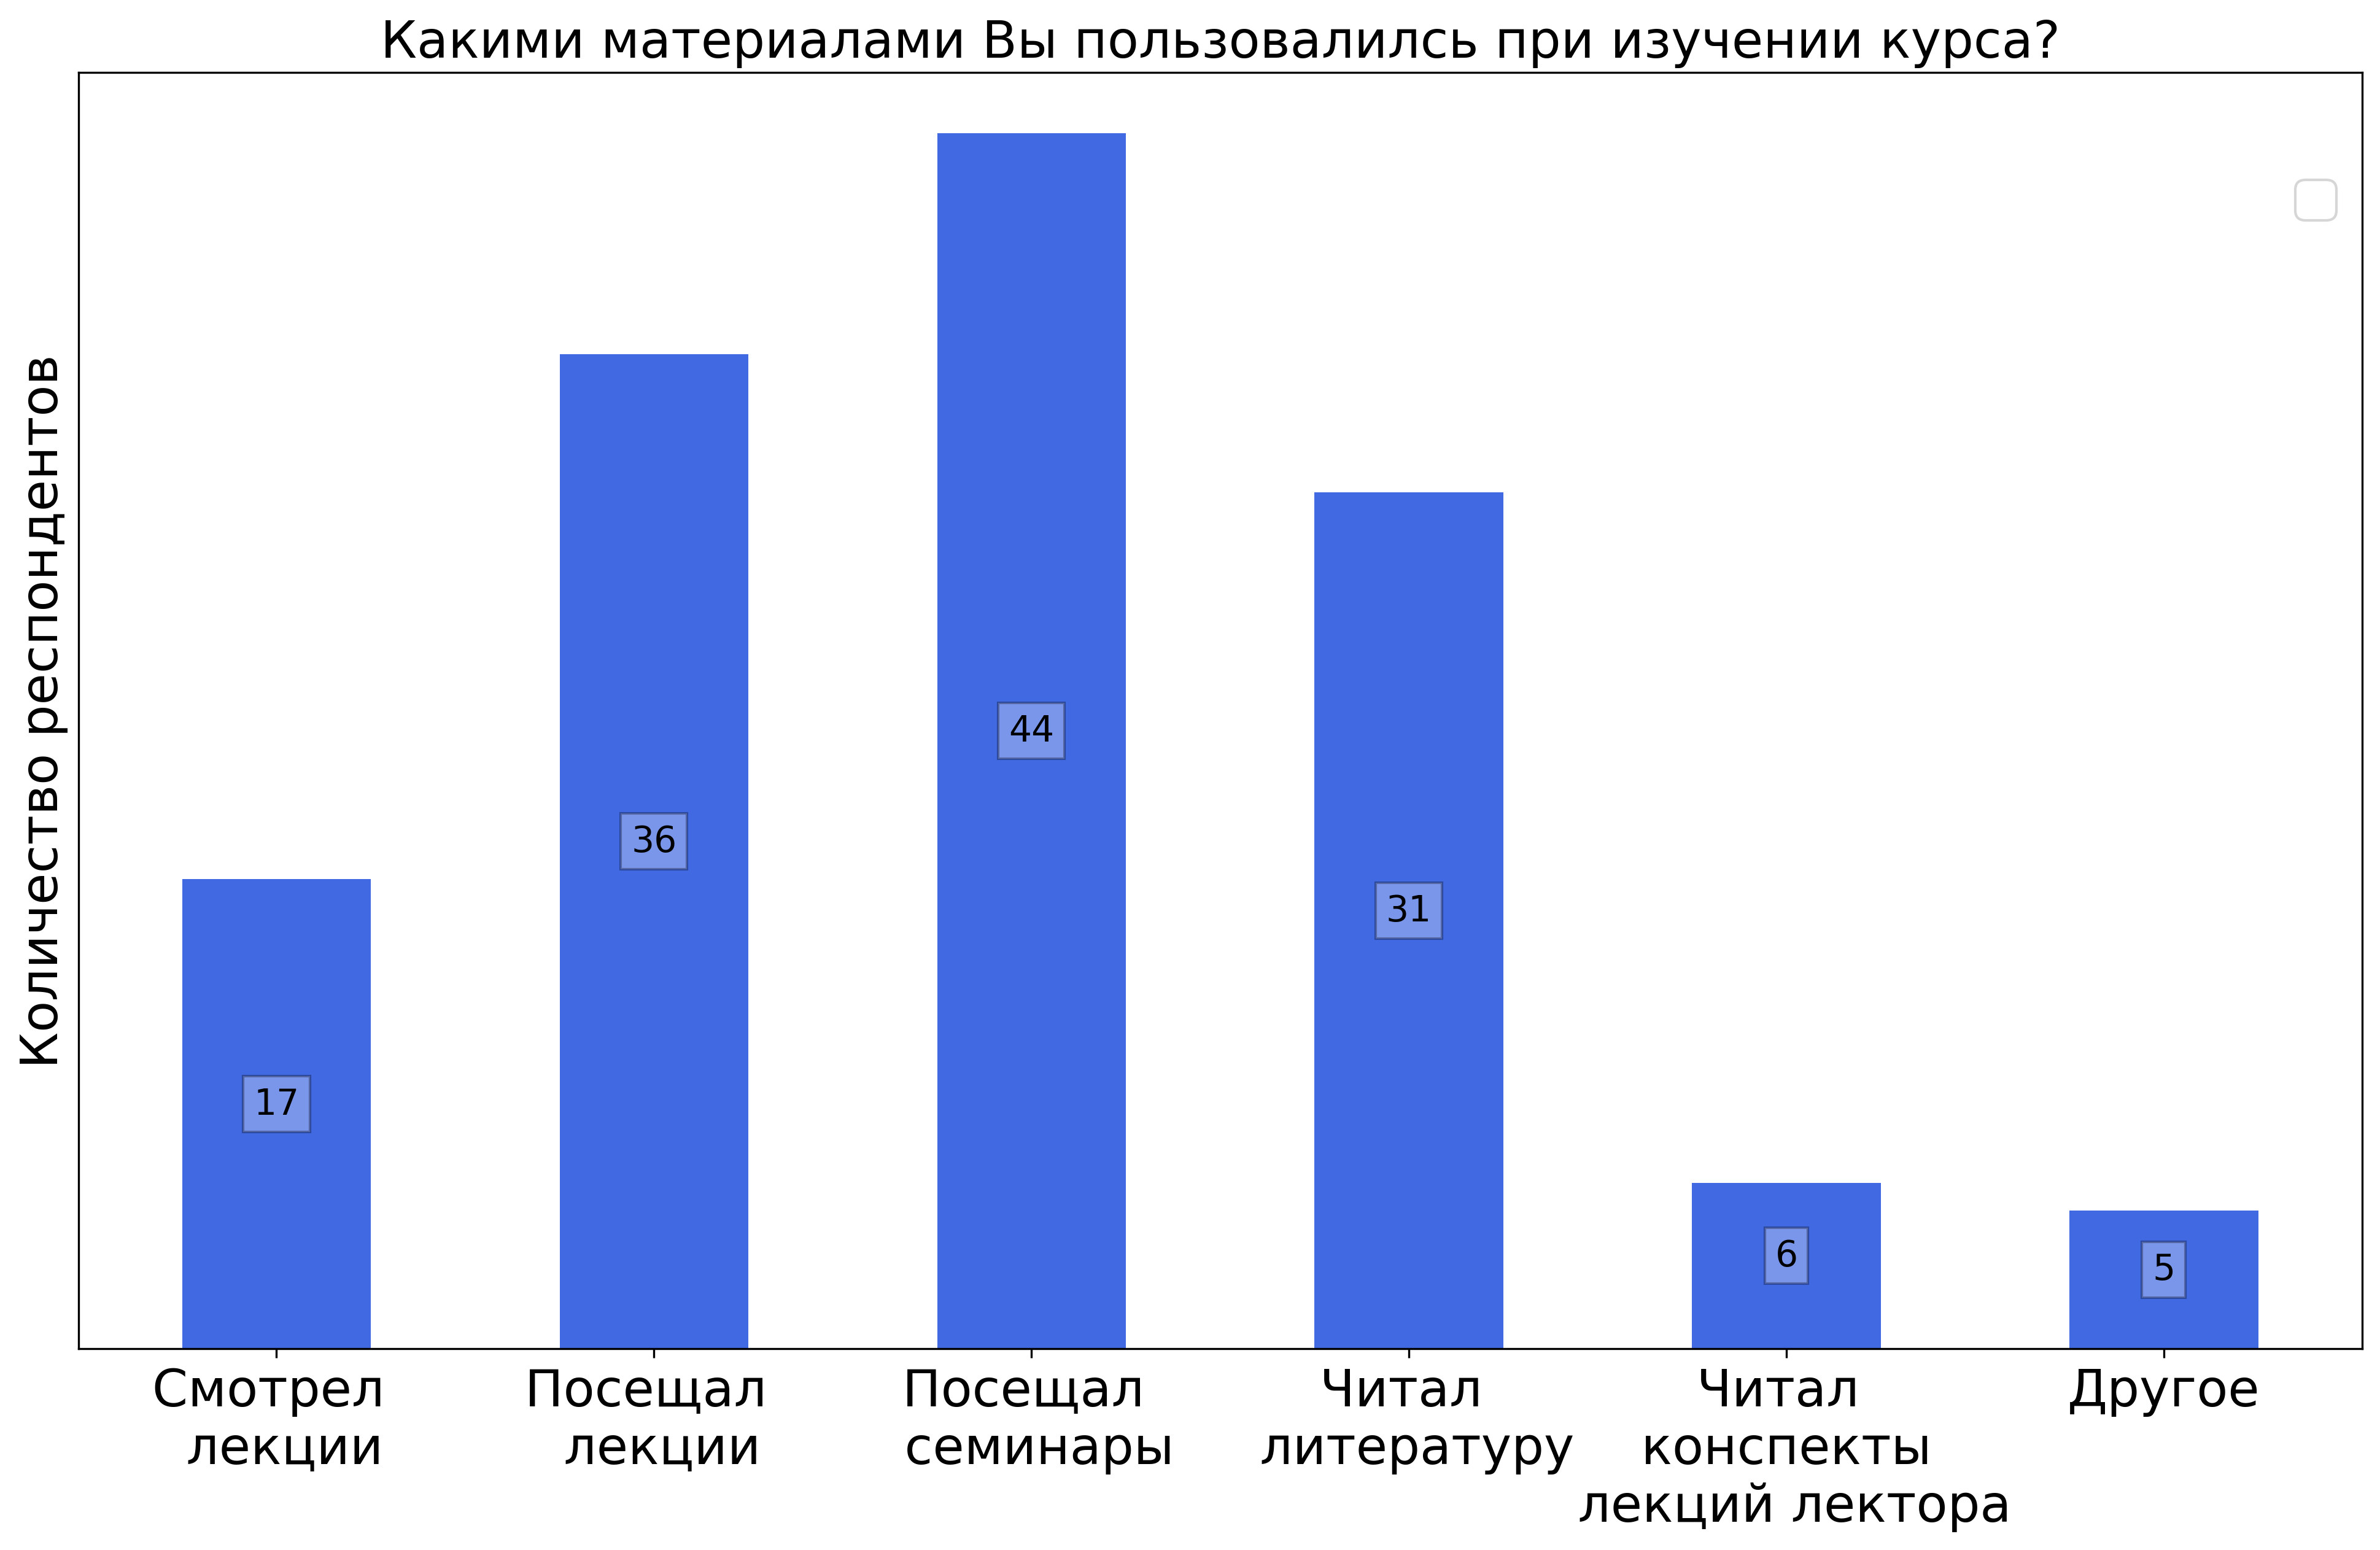
\includegraphics[width = 0.45\textwidth]{images/3 course/Аналоговая электроника/materials.png}
		\end{figure}

		\textit{В качестве других источников информации студенты указали:} 
		\begin{itemize}
			\item конспекты записей преподавателя по лабораторным работам;
			\item лекции Ларина А.Л. и Григорьева А.А.
		\end{itemize}

	\subsubsection{Отзыв студентов о лекциях. Лектор: Дунаева М.А.}

		\begin{figure}[H]
			\centering
            \begin{subfigure}[b]{0.45\textwidth}
				\centering
				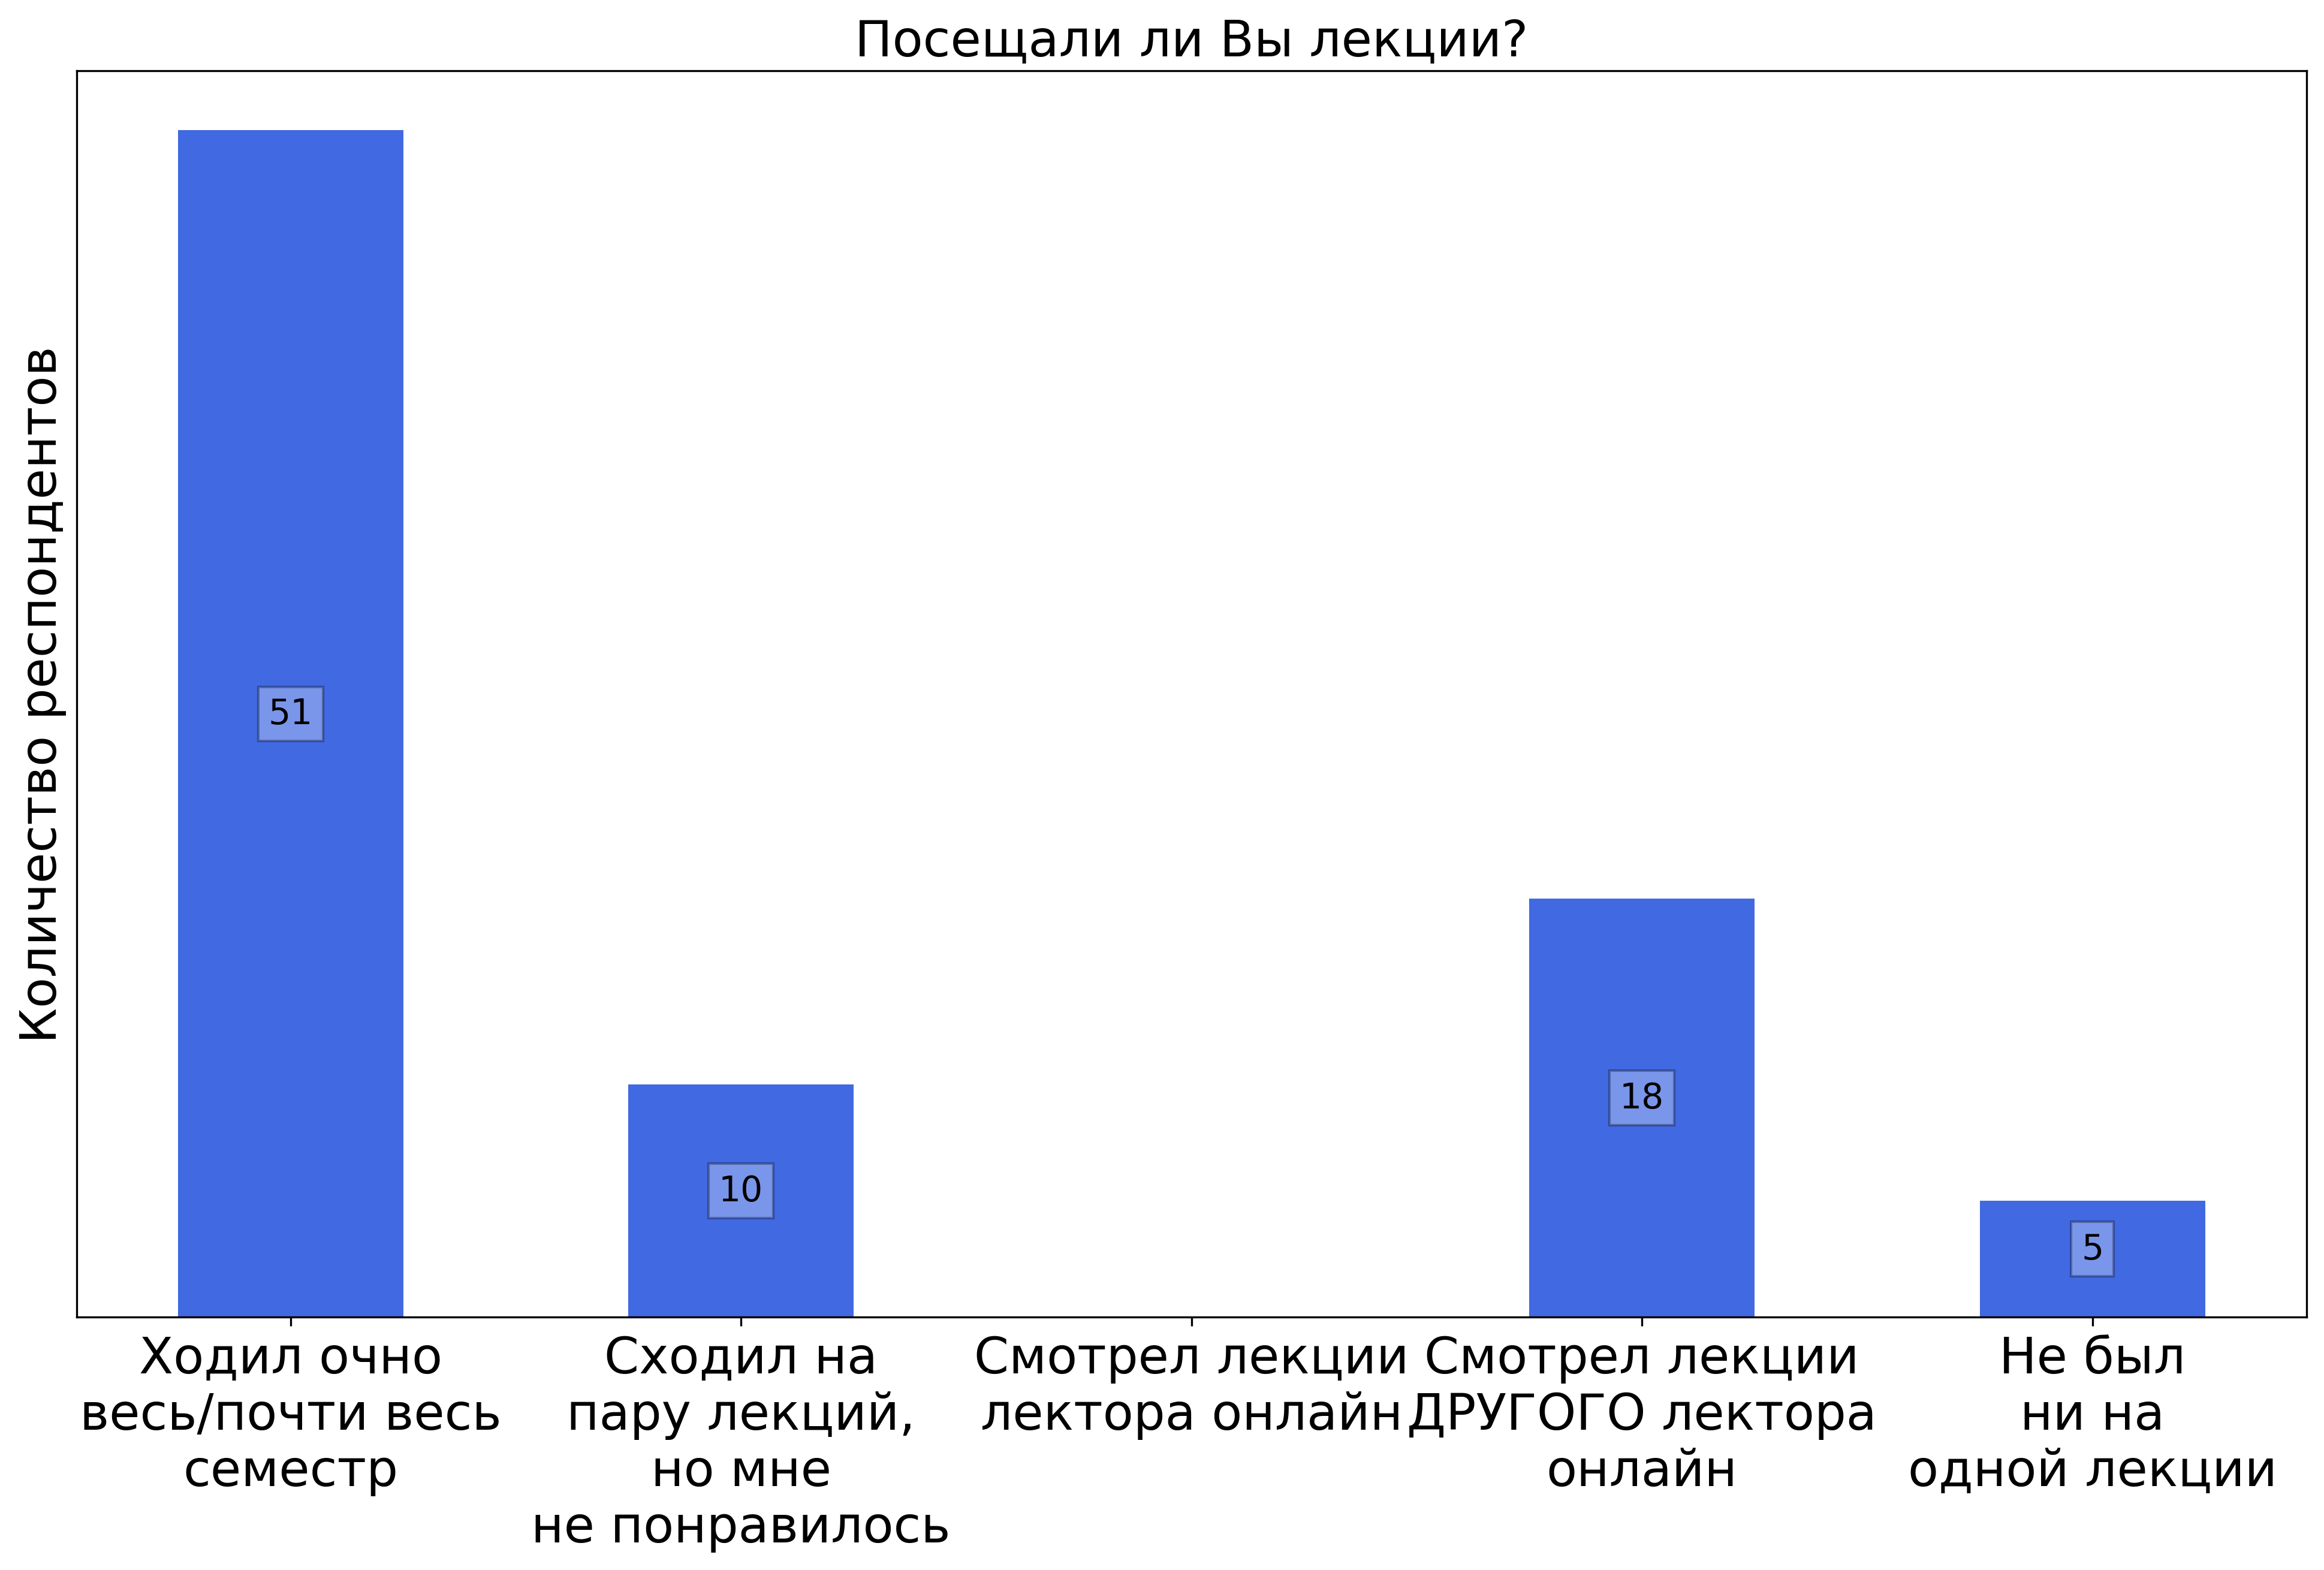
\includegraphics[width=\textwidth]{images/3 course/Аналоговая электроника/lecturer-questions-Дунаева М.А.-0.png}
			\end{subfigure}
			\begin{subfigure}[b]{0.45\textwidth}
				\centering
				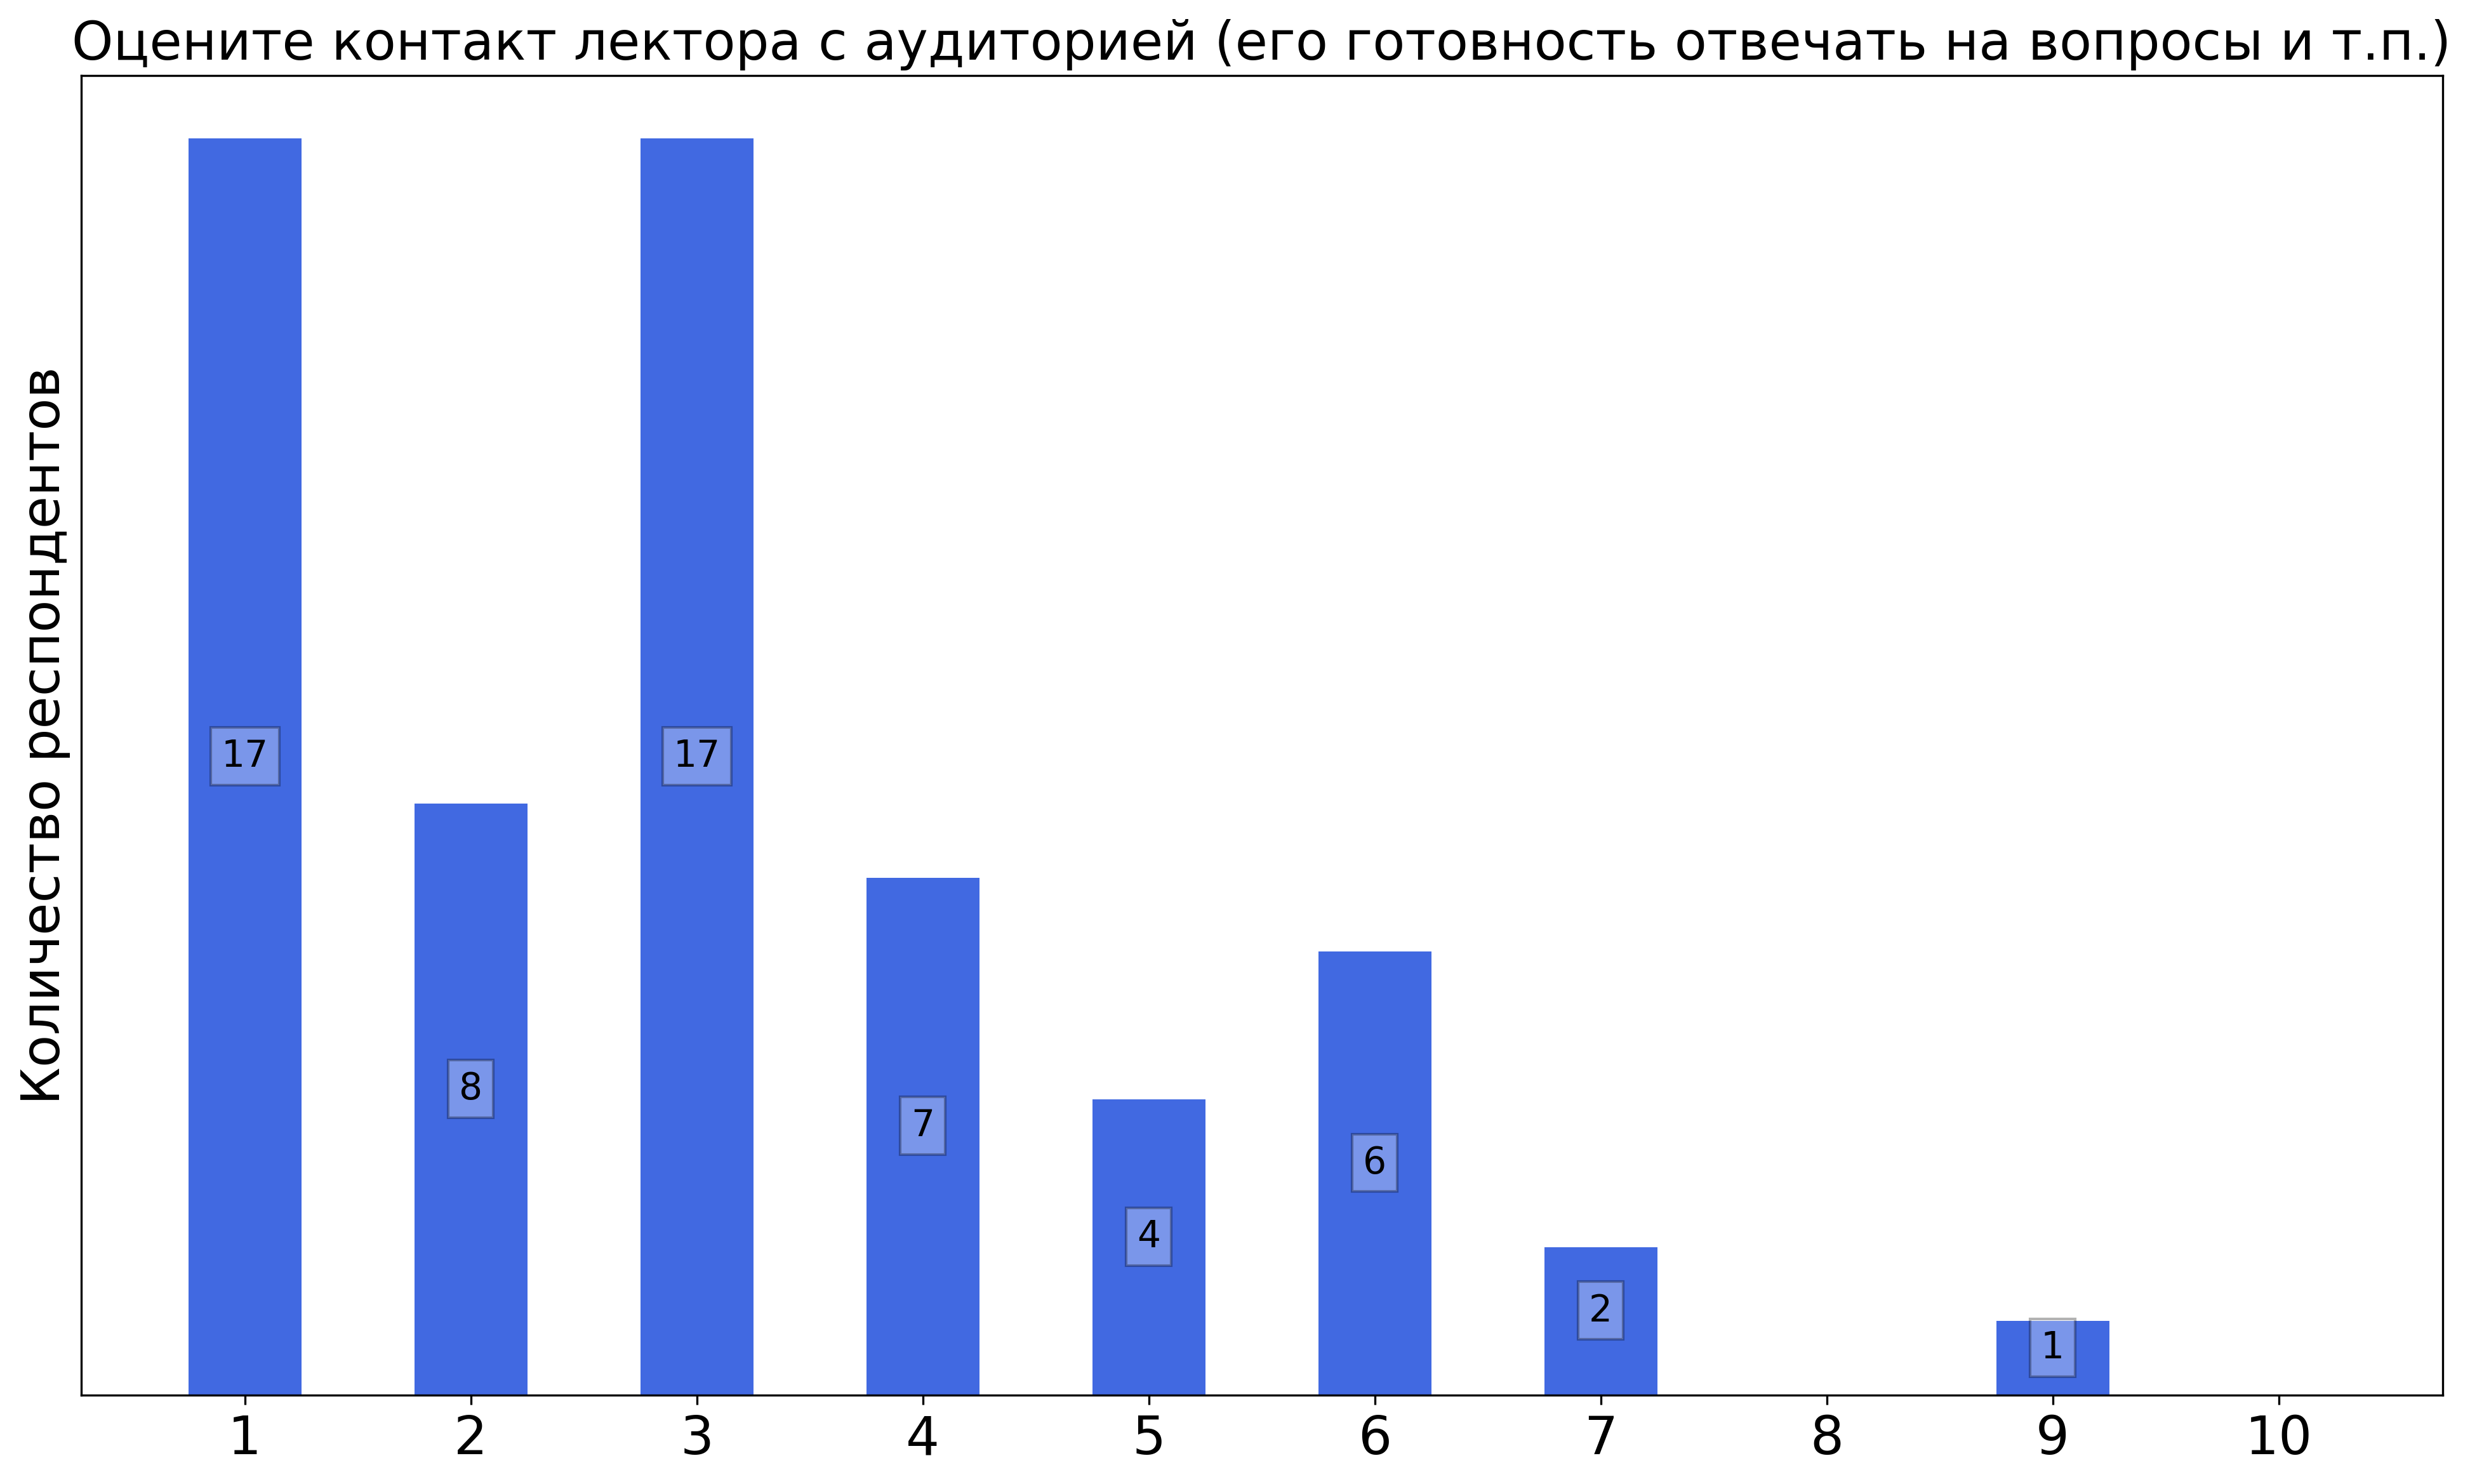
\includegraphics[width=\textwidth]{images/3 course/Аналоговая электроника/lecturer-marks-Дунаева М.А.-0.png}
			\end{subfigure}
			\begin{subfigure}[b]{0.45\textwidth}
				\centering
				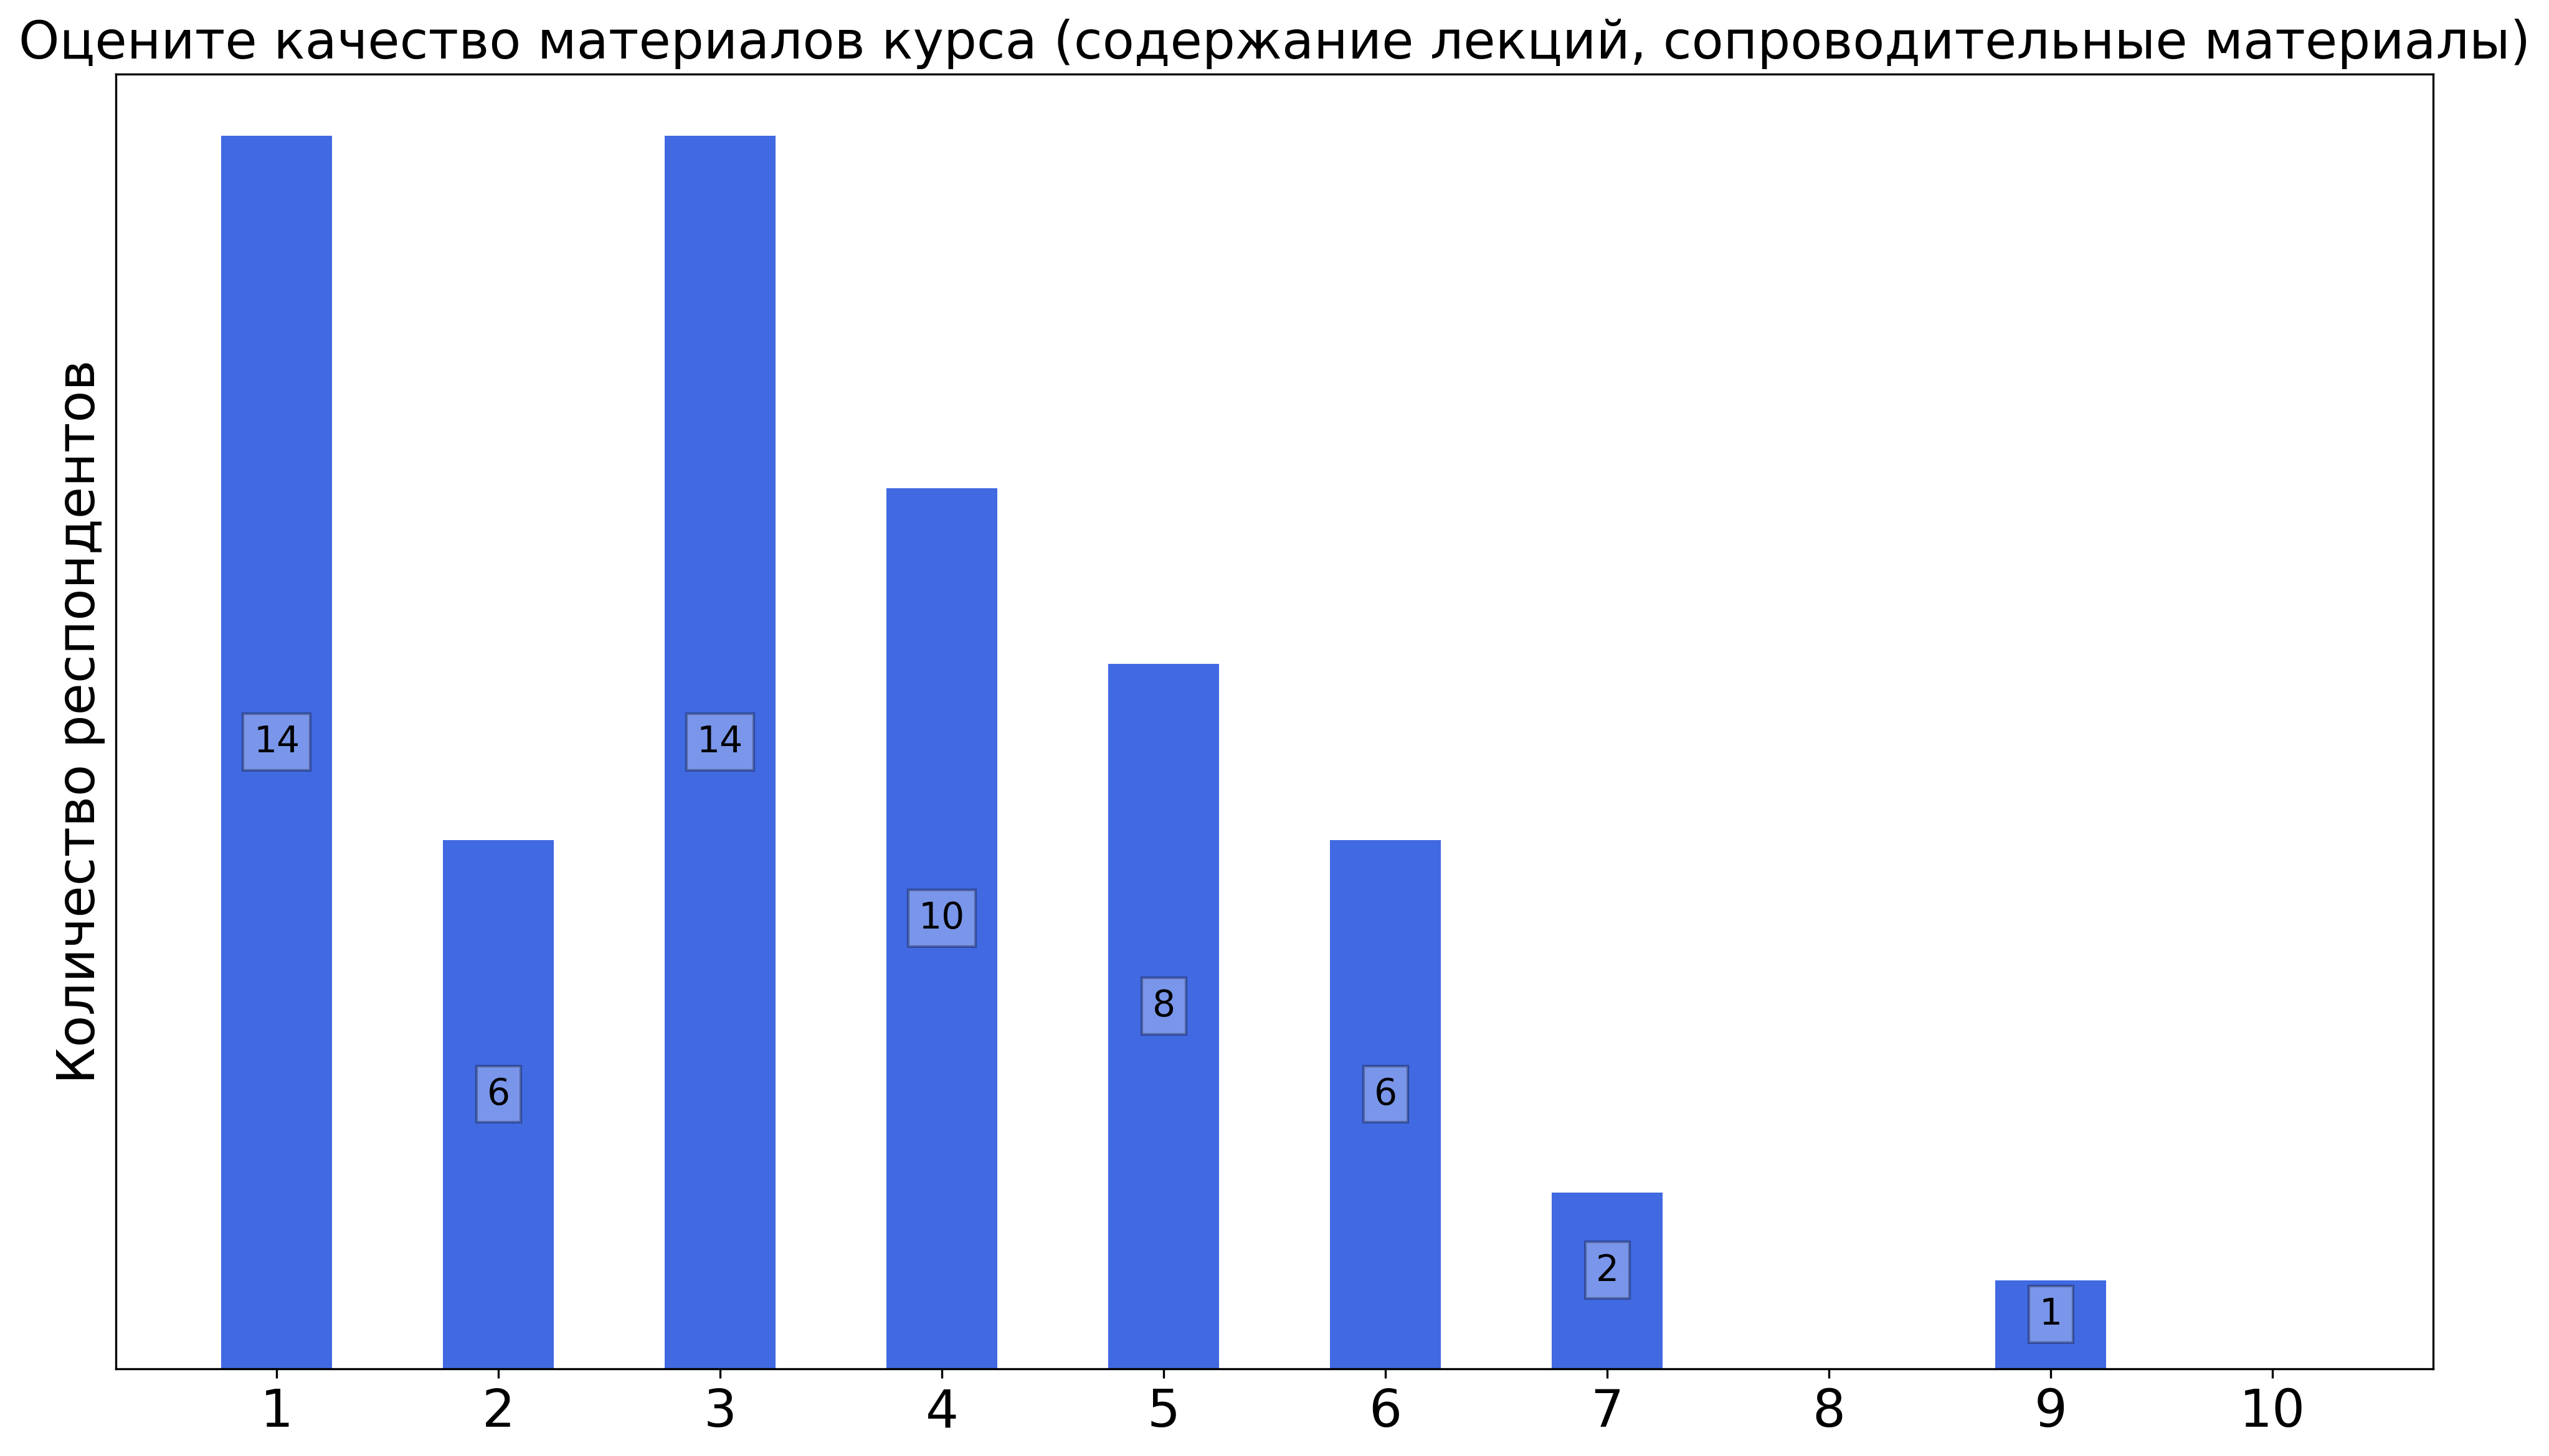
\includegraphics[width=\textwidth]{images/3 course/Аналоговая электроника/lecturer-marks-Дунаева М.А.-1.png}
			\end{subfigure}
			\begin{subfigure}[b]{0.45\textwidth}
				\centering
				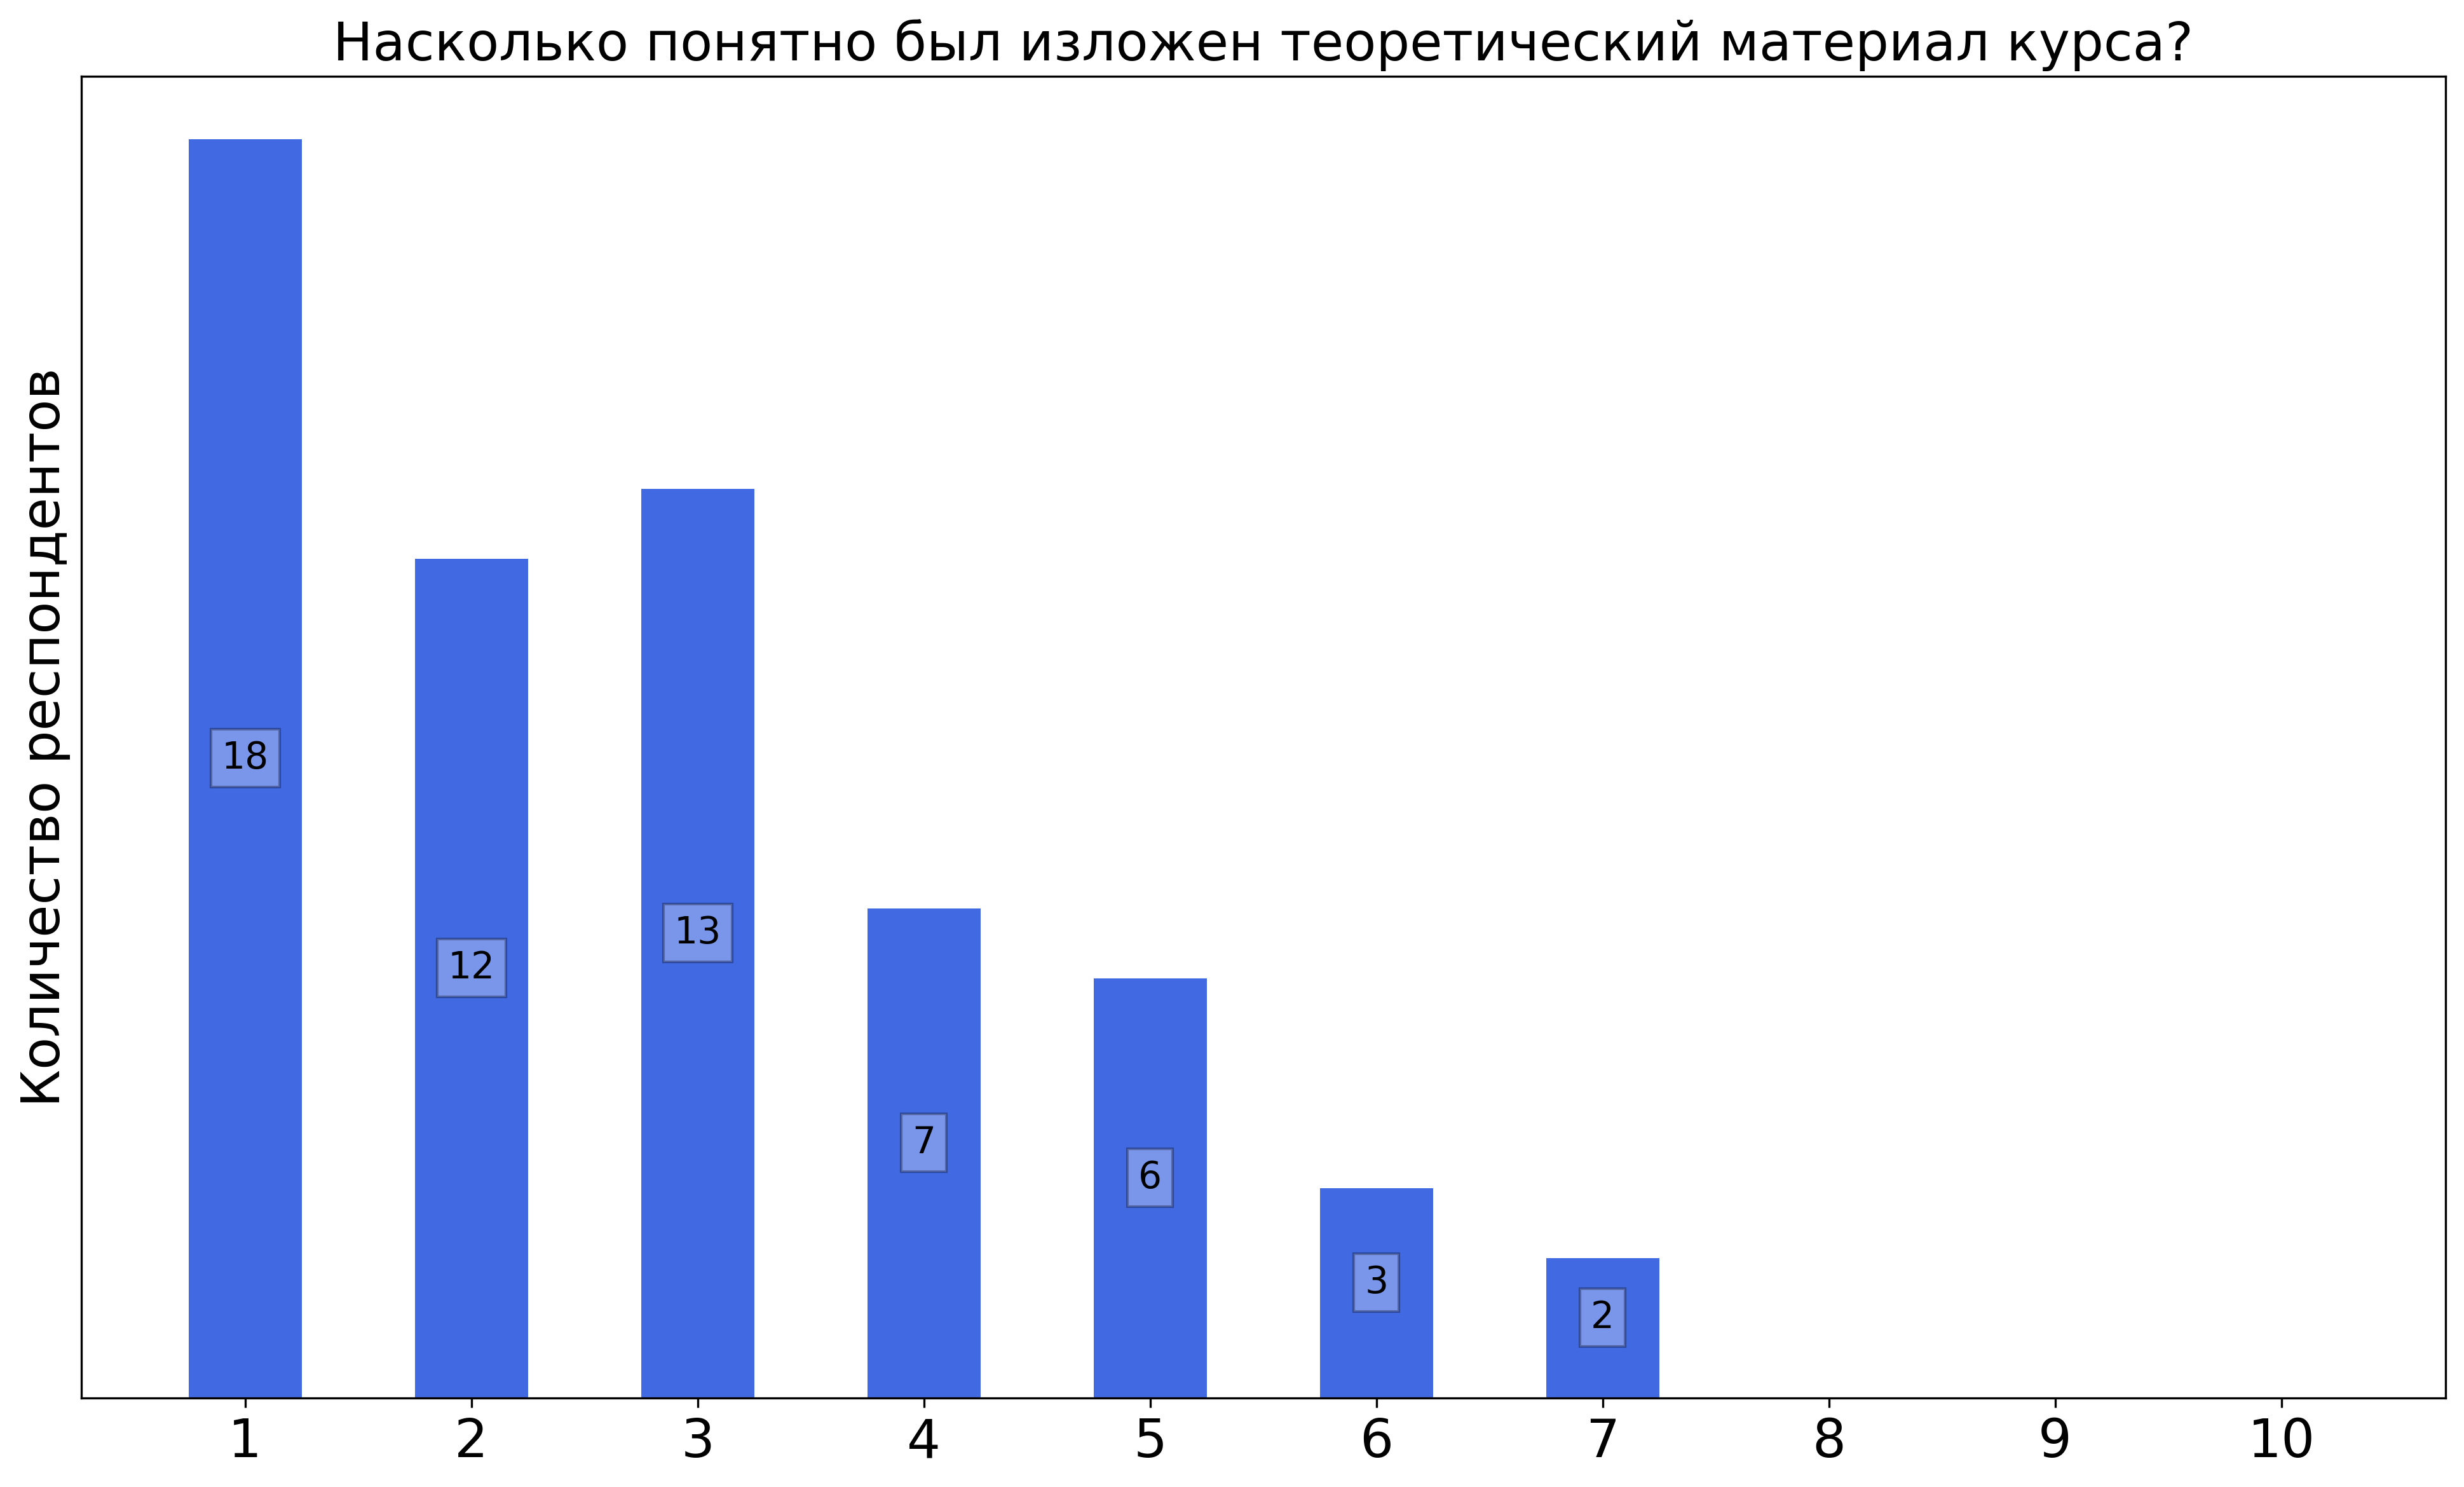
\includegraphics[width=\textwidth]{images/3 course/Аналоговая электроника/lecturer-marks-Дунаева М.А.-2.png}
			\end{subfigure}	
			\begin{subfigure}[b]{0.45\textwidth}
				\centering
				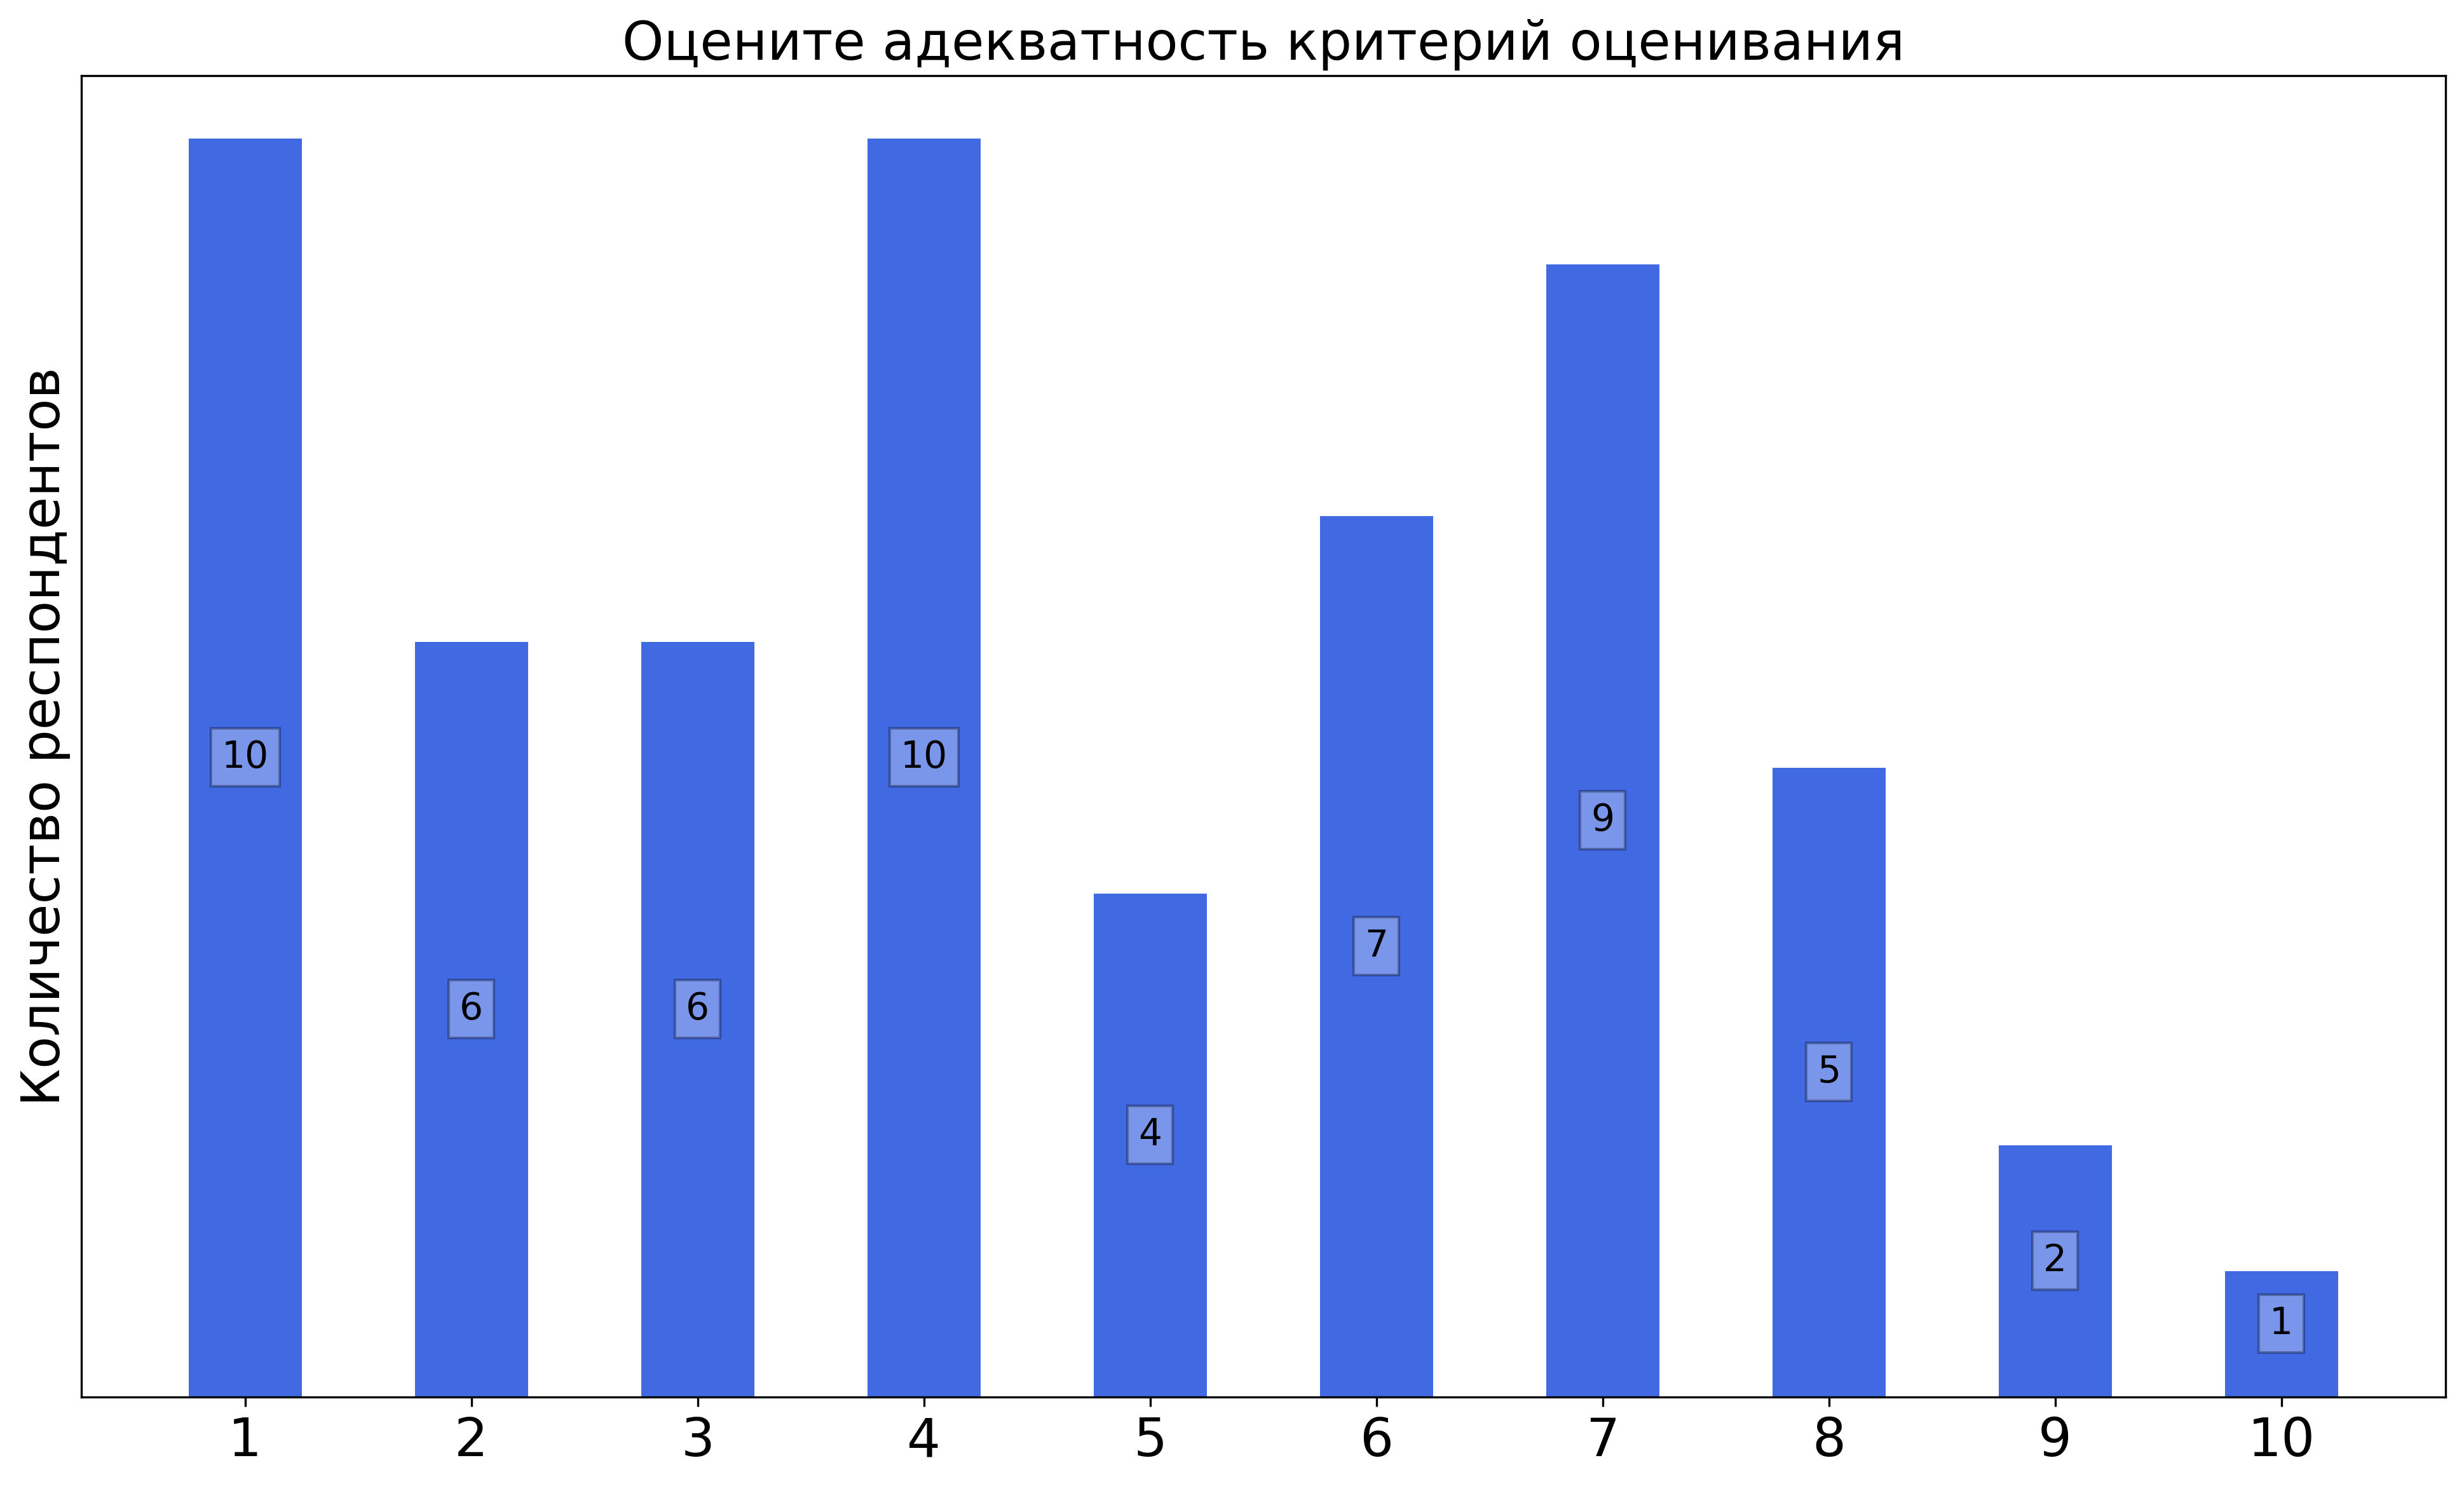
\includegraphics[width=\textwidth]{images/3 course/Аналоговая электроника/lecturer-marks-Дунаева М.А.-3.png}
			\end{subfigure}
			\caption{Оценки респондентов о качестве преподавания лекций по курсу <<Аналоговая электроника>>}
		\end{figure}

		\textbf{Комментарии студентов о лекциях\protect\footnote{сохранены оригинальные орфография и пунктуация}}
            \begin{commentbox} 
                Читает с листочка, может промолчать 20 минут, просто осознавая то, что написано на доске. Делаю вывод, что преподаватель к лекциям не готов 
            \end{commentbox} 
        
            \begin{commentbox} 
                К сожалению, Дунаева - худший лектор, с которым приходилось встречаться. На лекции ходили многие, чтобы катать в конце тесты и возможно получить автомат, слушали по-моему 2 человека из ее группы по лабам. Скорее всего, у лектора есть понимание материала, но просто нет преподавательского таланта, совсем. Спас нас Григорьев Александр Алексеевич, большая часть курса покрыта его записанными лекциями, иначе я не знаю, как закрыл бы лабы с нашим преподавателем (Бибиков).  
            \end{commentbox} 
        
            \begin{commentbox} 
                Отвратительный лектор при подаче материала. Непонятные условия оценивания при выставлении автоматов 
            \end{commentbox} 
        
            \begin{commentbox} 
                Лекции были скучные и не совсем понятные 
            \end{commentbox} 
        
            \begin{commentbox} 
                Классный лектор, который молчит 
            \end{commentbox} 
        
            \begin{commentbox} 
                Плохая готовность к лекциям, неспособность ответить на вопросы 
            \end{commentbox} 
        
            \begin{commentbox} 
                Непонятные от слова совсем лекции. Лектор выписывал информацию на доске и очень тихо объяснял их. На доп. вопросы четких ответов не было. Очень трудный для освоения курс. 
            \end{commentbox} 
        
            \begin{commentbox} 
                Очень уныло рассказывает, по сравнению с Григорьевым  
            \end{commentbox} 
        
            \begin{commentbox} 
                Создалось ощущение с первой лекции, что лектор не понимает о чём рассказывает. Говорит неуверенно, часто зависает надолго. Интерес к предмету был потерян быстро 
            \end{commentbox} 
        
            \begin{commentbox} 
                Порой создавалось ощущение, что лектор сама не понимает, что рассказывает; простейшие вопросы из аудитории вызывали двух-трехминутные задержки. Довольно быстро бесполезность очных лекций привела к тому, что большая часть потока просто проводила как-то время на лекции для того, чтобы сдать "летучку"(а порой люди и вовсе приходили только под конец лекции с листочком). По сути, весь курс ботался по записанным лекциям Ларина, у которого и сама программа выстроена как будто бы лучше, и подача приятнее. 
            \end{commentbox} 
        
            \begin{commentbox} 
                Совершенно непонятно что лектор рассказывает, часто по 10 минут смотрит в листочек и пытается понять, что там написано, плохо отвечает на вопросы. Слушать невозможно. Ужасный лектор. Для подготовки к сдачам ЛР смотрели лекуии Григорьева, на контрасте видно большую разницу в качестве лекций. 
            \end{commentbox} 
        
            \begin{commentbox} 
                Лекции никуда не годятся: видно, что лектор вообще не понимает предмета, пишет с листочка (скорее всего даже не своего) и долго всматривается в то, что написала. На вопросы не отвечала от слова "совсем".
                Из-за туманных обещаний автомата пришлось ходить весь семестр, в итоге раздача автомата происходила по известным лишь одному лектору правилам 
            \end{commentbox} 
        
            \begin{commentbox} 
                Иногда кажется, что она сама не понимает курс. Довольна добрая, что положительно выделяет на фоне Филатова. Однако курс все еще абсолютно непонятен. Расстраивает фактически обязательное посещение лекций (кажется, основной критерий на автомат, ибо тесты, кажется, проверяются довольно рандомно) 
            \end{commentbox} 
        
            \begin{commentbox} 
                Не редко после какого-либо вопроса по теме лекций, преподаватель, помычав, давала ответ из ряда: "Ну тут на доске всё написано, должно быть очевидно". Было невозможно слушать лекции из-за плохого разъяснения материала. 
            \end{commentbox} 
        
            \begin{commentbox} 
                Невнятно объясняет, слушать невозможно  
            \end{commentbox} 
        
            \begin{commentbox} 
                Абсолютно бесполезные лекции, ничего не понятно 
            \end{commentbox} 
        
            \begin{commentbox} 
                Не особо я слушала, просто приходила, тк нада. Не считаю этот предмет полезным лично для себя 
            \end{commentbox} 
        
            \begin{commentbox} 
                Было тяжело слушать, я вначале попробовал, но в итоге забросил это дело. Лариновский курс лекций прям зашёл (я ценитель) 
            \end{commentbox} 
        
            \begin{commentbox} 
                Не готова к лекциям. Рассказывается сухо, всё время спиной к аудитории. Не сложилось впечатление полноты курса, зачем мы это делаем. 
            \end{commentbox} 
        
            \begin{commentbox} 
                Сложилось впечатление, что лектор с трудом сможет сформулировать закон Ома. Готовность к лекциям нулевая, отношение к своей работе такое же. Как в вузе такого уровня могут преподавать такие специалисты?) 
            \end{commentbox} 
        
            \begin{commentbox} 
                Худший лектор за всю историю моей учёбы на Физтехе. Складывается впечатление, что она сама не понимает, что рассказывает. Стыдно, что на факультете радиотехники такие преподаватели. Из-за этого всё, что связано с радиотехникой и в целом содержит приставку "радио" в учебном плане, вызывает стойкое отвращение.  
            \end{commentbox} 
        
            \begin{commentbox} 
                Лектор не слишком активный в контакте с аудиторией. Плохо готовит к лабораторным 
            \end{commentbox} 
        
            \begin{commentbox} 
                Если по-честному, то я мало чего вынесла с лекций по аналоговой электронике. Основную массу знаний я черпала из лабораторных работ, хотя осталось довольно много пробелов в понимании предмета. Товарищ Дунаева, насколько я понимаю, читает лекции впервые, поэтому получается плохо. Понятно, что читать лекции на весь поток это отдельное искусство и нужно много опыта у преподавателя. Но студенту важно разобраться, понять, вынести какие-то знания с лекции. Здесь это невозможно. Вся лекция - практически молчание, не особо связанные фразы, объяснения как и почему что-либо работает неясны. Я хочу хорошего, опытного лектора((( Потому что сейчас мы ходим на лекции лишь для того, чтобы в конце написать тестик и в конце, возможно, получить автомат. 
            \end{commentbox} 
        
            \begin{commentbox} 
                Лектор никакой. Это с одной стороны, позволяет ничего не делать на предмете. С другой, для тех кто хочет разобраться - это капец, не поймете ничего. Дудаева, такое ощущение, лекции пишет для себя. 
            \end{commentbox} 
        
            \begin{commentbox} 
                К сожалению, такое ощущение, что идет «зачитывание материала по листочку». Иногда лектор может потерять мысль и 5-10 минут пытаться  вернуться в нужное русло. Также была довольно неприятная ситуация с летучками, которые были необходимым условием для получения автомата: у некоторых людей было так, что ответы одинаковые, однако у одного был плюс за это задание, а у другого - минус. Из-за этого было немало людей, которые действительно старались и имели «отлично» по лабораторным работам, однако автомат не получили вследствие этой странной системы оценивания летучек. 
            \end{commentbox} 
        
            \begin{commentbox} 
                Очень плохие лекции - крайне тихо, каждые 5 минут лектор "зависает", смотря в свой листочек по несколько минут, путается в рисунках, уследить мысль невозможно. Оценивание самостоятельных работ в конце лекций - рандом 
            \end{commentbox} 
        
            \begin{commentbox} 
                Подача материала сумбурная. Лектор иногда сам долго смотрит в доску и что-то пытается понять. На вопросы аудитории ответы очень расплывчатые   
            \end{commentbox} 
        
            \begin{commentbox} 
                Отвратительный курс лекций, который к тому же нужно посещать для получения автомата. Лектор ужасно излагает материал, вводя новые понятия из ниоткуда. На вопросы же о том, чем является тот или иной параметр, Дунаева просто ищет ответ в своей тетради, зачитывает название и идёт дальше. Бывает такое, что лектор останавливается и не знает, что дальше сказать, подготовка к лекциям и качества изложения ужасны. Понять с лекций хоть что-либо попросту невозможно, а их обязательное посещение для получения автомата и вовсе превращает их в пытку. В процессе обучения для сдачи лабораторных работ всегда приходилось смотреть лекции Ларина или Григорьева, в которых материал излагается несравнимо лучше. Особенно хороши лекции Григорьева, очень жаль, что конкретно данный курс он никогда не вёл, поэтому приходилось смотреть лекции по соответствующим темам из других курсов. 
            \end{commentbox} 
        
            \begin{commentbox} 
                Смотрел записи лекций Григорьева для ФАКИ и пару раз полностью отсидел на Дунаевой (не приходил в конце пары чисто отметиться) 
            \end{commentbox} 
        
            \begin{commentbox} 
                Складывается впечатление, что лектор сам не понимает излагаемый материал, постоянно спотыкался, все лекция с листочка, происходили минутные молчаливые паузы в попытках разобрать лектором, что написано. Ответы на вопросы неразборчивые и уклончивые, энтузиазм вести лекции у преподавателя отсутствует. Мини-тесты, из-за которых приходилось посещать лекции ради автомата, проверялись не пойми как (вместе со знакомым сдавали идентичные решения на каждой лекции, но оценки разные). Условия автомата достаточно строгие - >7 за лекции и отл на лабах (почти невыполнимое на некоторых лабниках условие). 
            \end{commentbox} 
        
            \begin{commentbox} 
                Объясняет довольно медленно, на вопросы отвечает, думая, что неплохо. Только очень медленно 
            \end{commentbox} 
        
            \begin{commentbox} 
                Был на первой лекции, очень не понравилось и не стал ходить, несмотря на наличие системы "автоматов". Лектор читает с бумажки и не может толком донести тему лекции, ответить на вопросы студентов. Смотрел курсы лекций А.А.Григорьева и Ларина в записи и читал методические материалы, плюс для понимания очень помогли практические занятия в лабаратории с Р.А.Зариповым, к которому перевёлся так же от М.А.Дунаевой. 
            \end{commentbox} 
        
            \begin{commentbox} 
                Посещал лекции Григорьева И. А. для факи (то же курс аналоговой электроники), вынес оттуда куда больше нежели на курсе Дунаевой, материал излагался понятней и структурированней. 
            \end{commentbox} 
        
            \begin{commentbox} 
                Как лектор ужасна, путается, зависает, иногда не может ответить на вопросы. Никак не выражает заинтересованность, как делают другие лекторы. Смотрел Григорьева в записи. 
            \end{commentbox} 
        
            \begin{commentbox} 
                Невозможно слушать, постоянные паузы, невозможность ответить на вопросы, смотрел Григорьева. 
            \end{commentbox} 
        
            \begin{commentbox} 
                Дунаева читает очень непонятно, критерии для автоматов тоже странные. На каждой лекции были тесты, у многих людей, которые писали тесты вместе в конце вышли разные оценки. По лекциям Дунаевой заботать материал невозможно, поэтому весь семестр смотрела лекции Григорьева. 
            \end{commentbox} 
        
            \begin{commentbox} 
                Очень плохое объеснение на лекциях. Фактически его просто нет.  Лектор просто перерисовывает схемы и некотрые формулы без вывода со своей тетради на доску, иногда подолгу стоя на месте и проверяя свои же записи, студенты часто поправляют.  Если брать в сравнение лекции Ларина, то у него всегда есть презентации, чтобы не тратить время на перерисовывание  больших схем.  Поэтому и объяснить он успевает больше : как работает схема,  какие  токи куда текут, какие где напряжения  и тп. Наш лектор этого, от слова сосем, не делает. Формулы , написанные лектором на доске, никак не поясняют работу схемы.  Также лектор дает задачи  в конце каждой лекции. В конце семестра оценка за задачи учитывается при выставлении автомата вместе с оценкой за лабораторные. Задачи, даваемые на лекции, не сопостовимы по сложности со сдачей лабораторной. Они совершенно ничего не говорят о знании человеком предмета в отличие от сдачи лабороторной. Кроме того, не ясны критерии оценивания. У разных студентов  с одинаковым ответом, могут стоять совсем разные баллы. Лектор не раздает проверенные задачи, тем самым невозможно проверить, что было не так в решении. Еще стоит рассмотреть такую ситуацию:  даже у тех студентов, у которых отл. за лабораторные, стоят меньшие баллы, по сравнению с теми у кого хор. и ниже. Хотя  по логике, как я описал выше, сдав лабораторные на отл. , студент должен знать больше, чем тот который сдал на хор., а значит у  первого должна быть оценка за лекционные задачи выше( ведь чтобы сдать лабораторную так хорошо, он должен был разобраться в теме и он не может не решить эти простейшие задачи, котрые дает лектор), чем у второго, но это часто не так. Это наводит на мысли об адекватности такого критерия оценивания как лекционные задачи. Можно задаться вопросом, что они ,вообще, проверяют.  Уровень знаний , как мы выяснили, - нет. Может быть это попытка, отмечать посещаемость. Но это тоже не так, так как есть случаи, что некотрые студенты просто приходят специально к концу лекции, чтобы сдать задачу и получить балл и получают его, а те кто честно был лекции с самого начало могут его не получить. Если лектору так нужна эта процедура с проверкой знаний(хотя о их количестве трудно говорить), полученных  студентом на лекции можно взять пример из Компюьтерных сетей, котрые вел у нас Климанов Максим Михайлович. Он опубликовывал результаты каждого такого тестика с пофамильным списком и баллами, и раздавал проверенные работы, можно было подойти и спросить, что не так. При выставлении оценки , эти тесты входили в очень маленьком процентом соотношении (5\%). Кроме того, они были не каждую лекцию, а были про пройденному материалы нескольких предыдущих лекций. А на аналоговой электроники лекционные задачи, вносят по итогу слишком большую неопределенность и несправедливость в выставлении итоговых оценок и автоматов. 
            \end{commentbox}

            
    \subsubsection{Отзыв студентов о лабораторных работах. Преподаватель: Арумов Г.П.}
		\begin{figure}[H]
			\centering
			\begin{subfigure}[b]{0.45\textwidth}
				\centering
				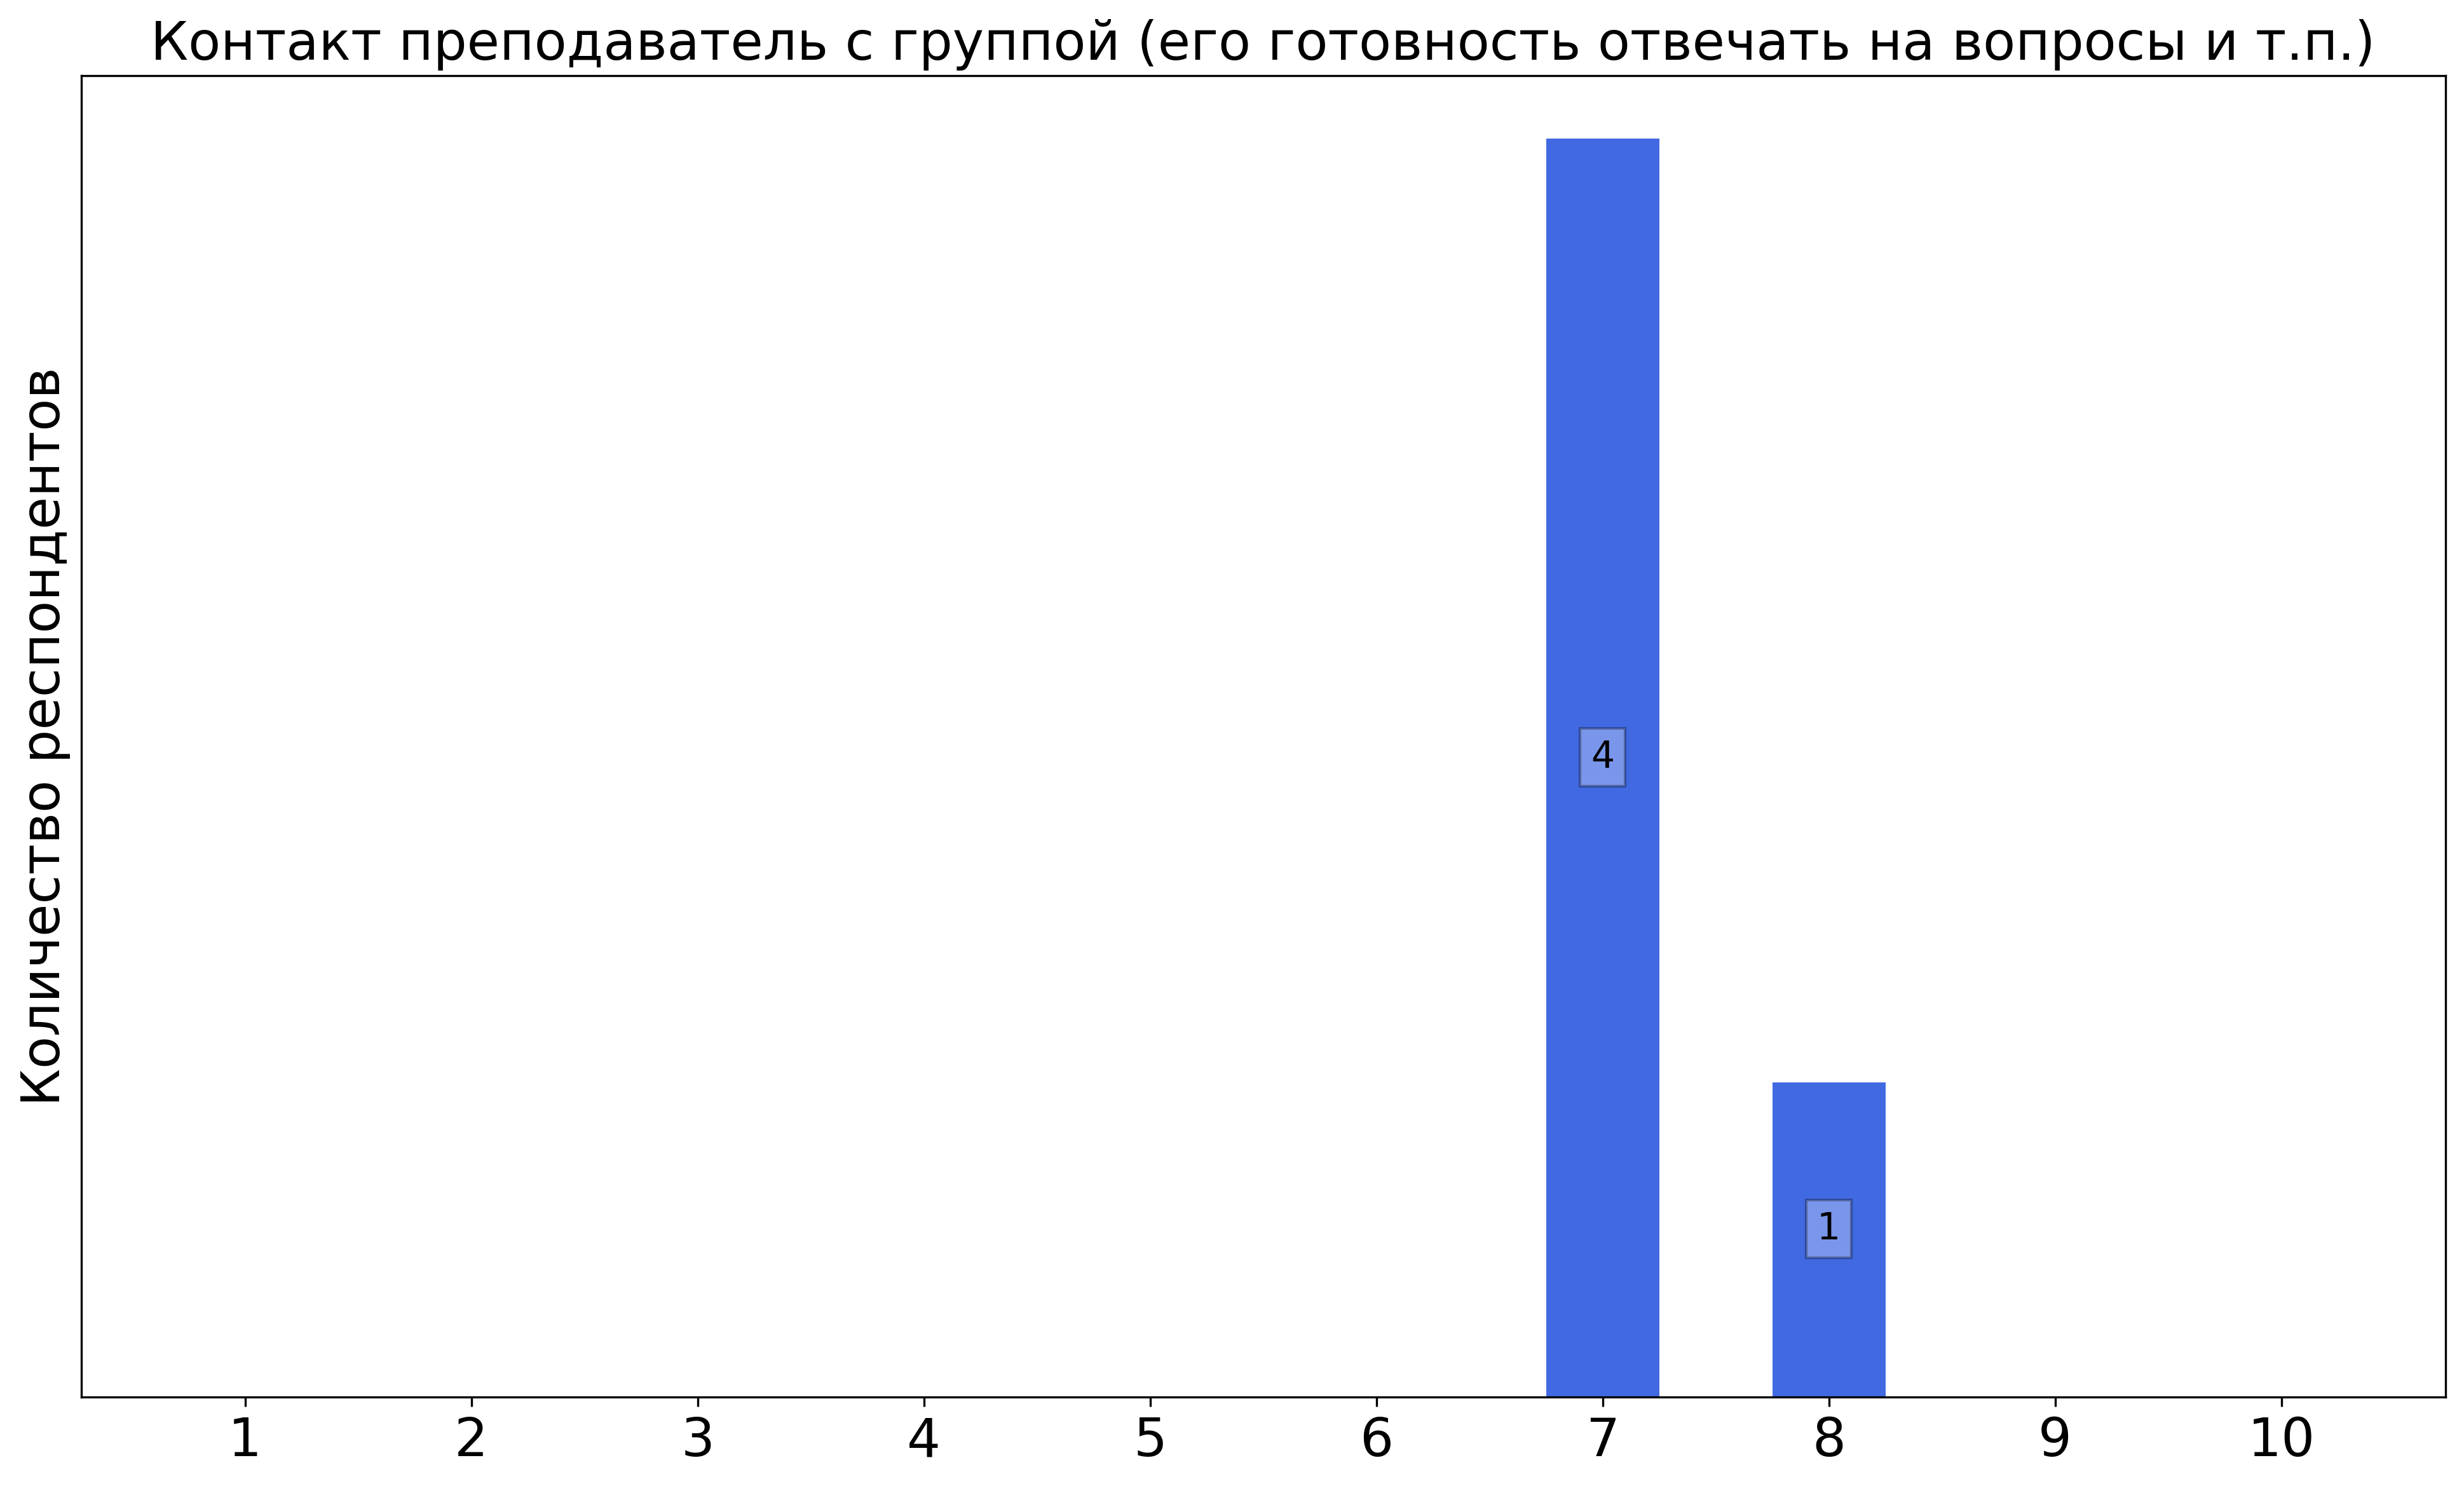
\includegraphics[width=\textwidth]{images/3 course/Аналоговая электроника/labniks-marks-Арумов Г.П.-0.png}
			\end{subfigure}
			\begin{subfigure}[b]{0.45\textwidth}
				\centering
				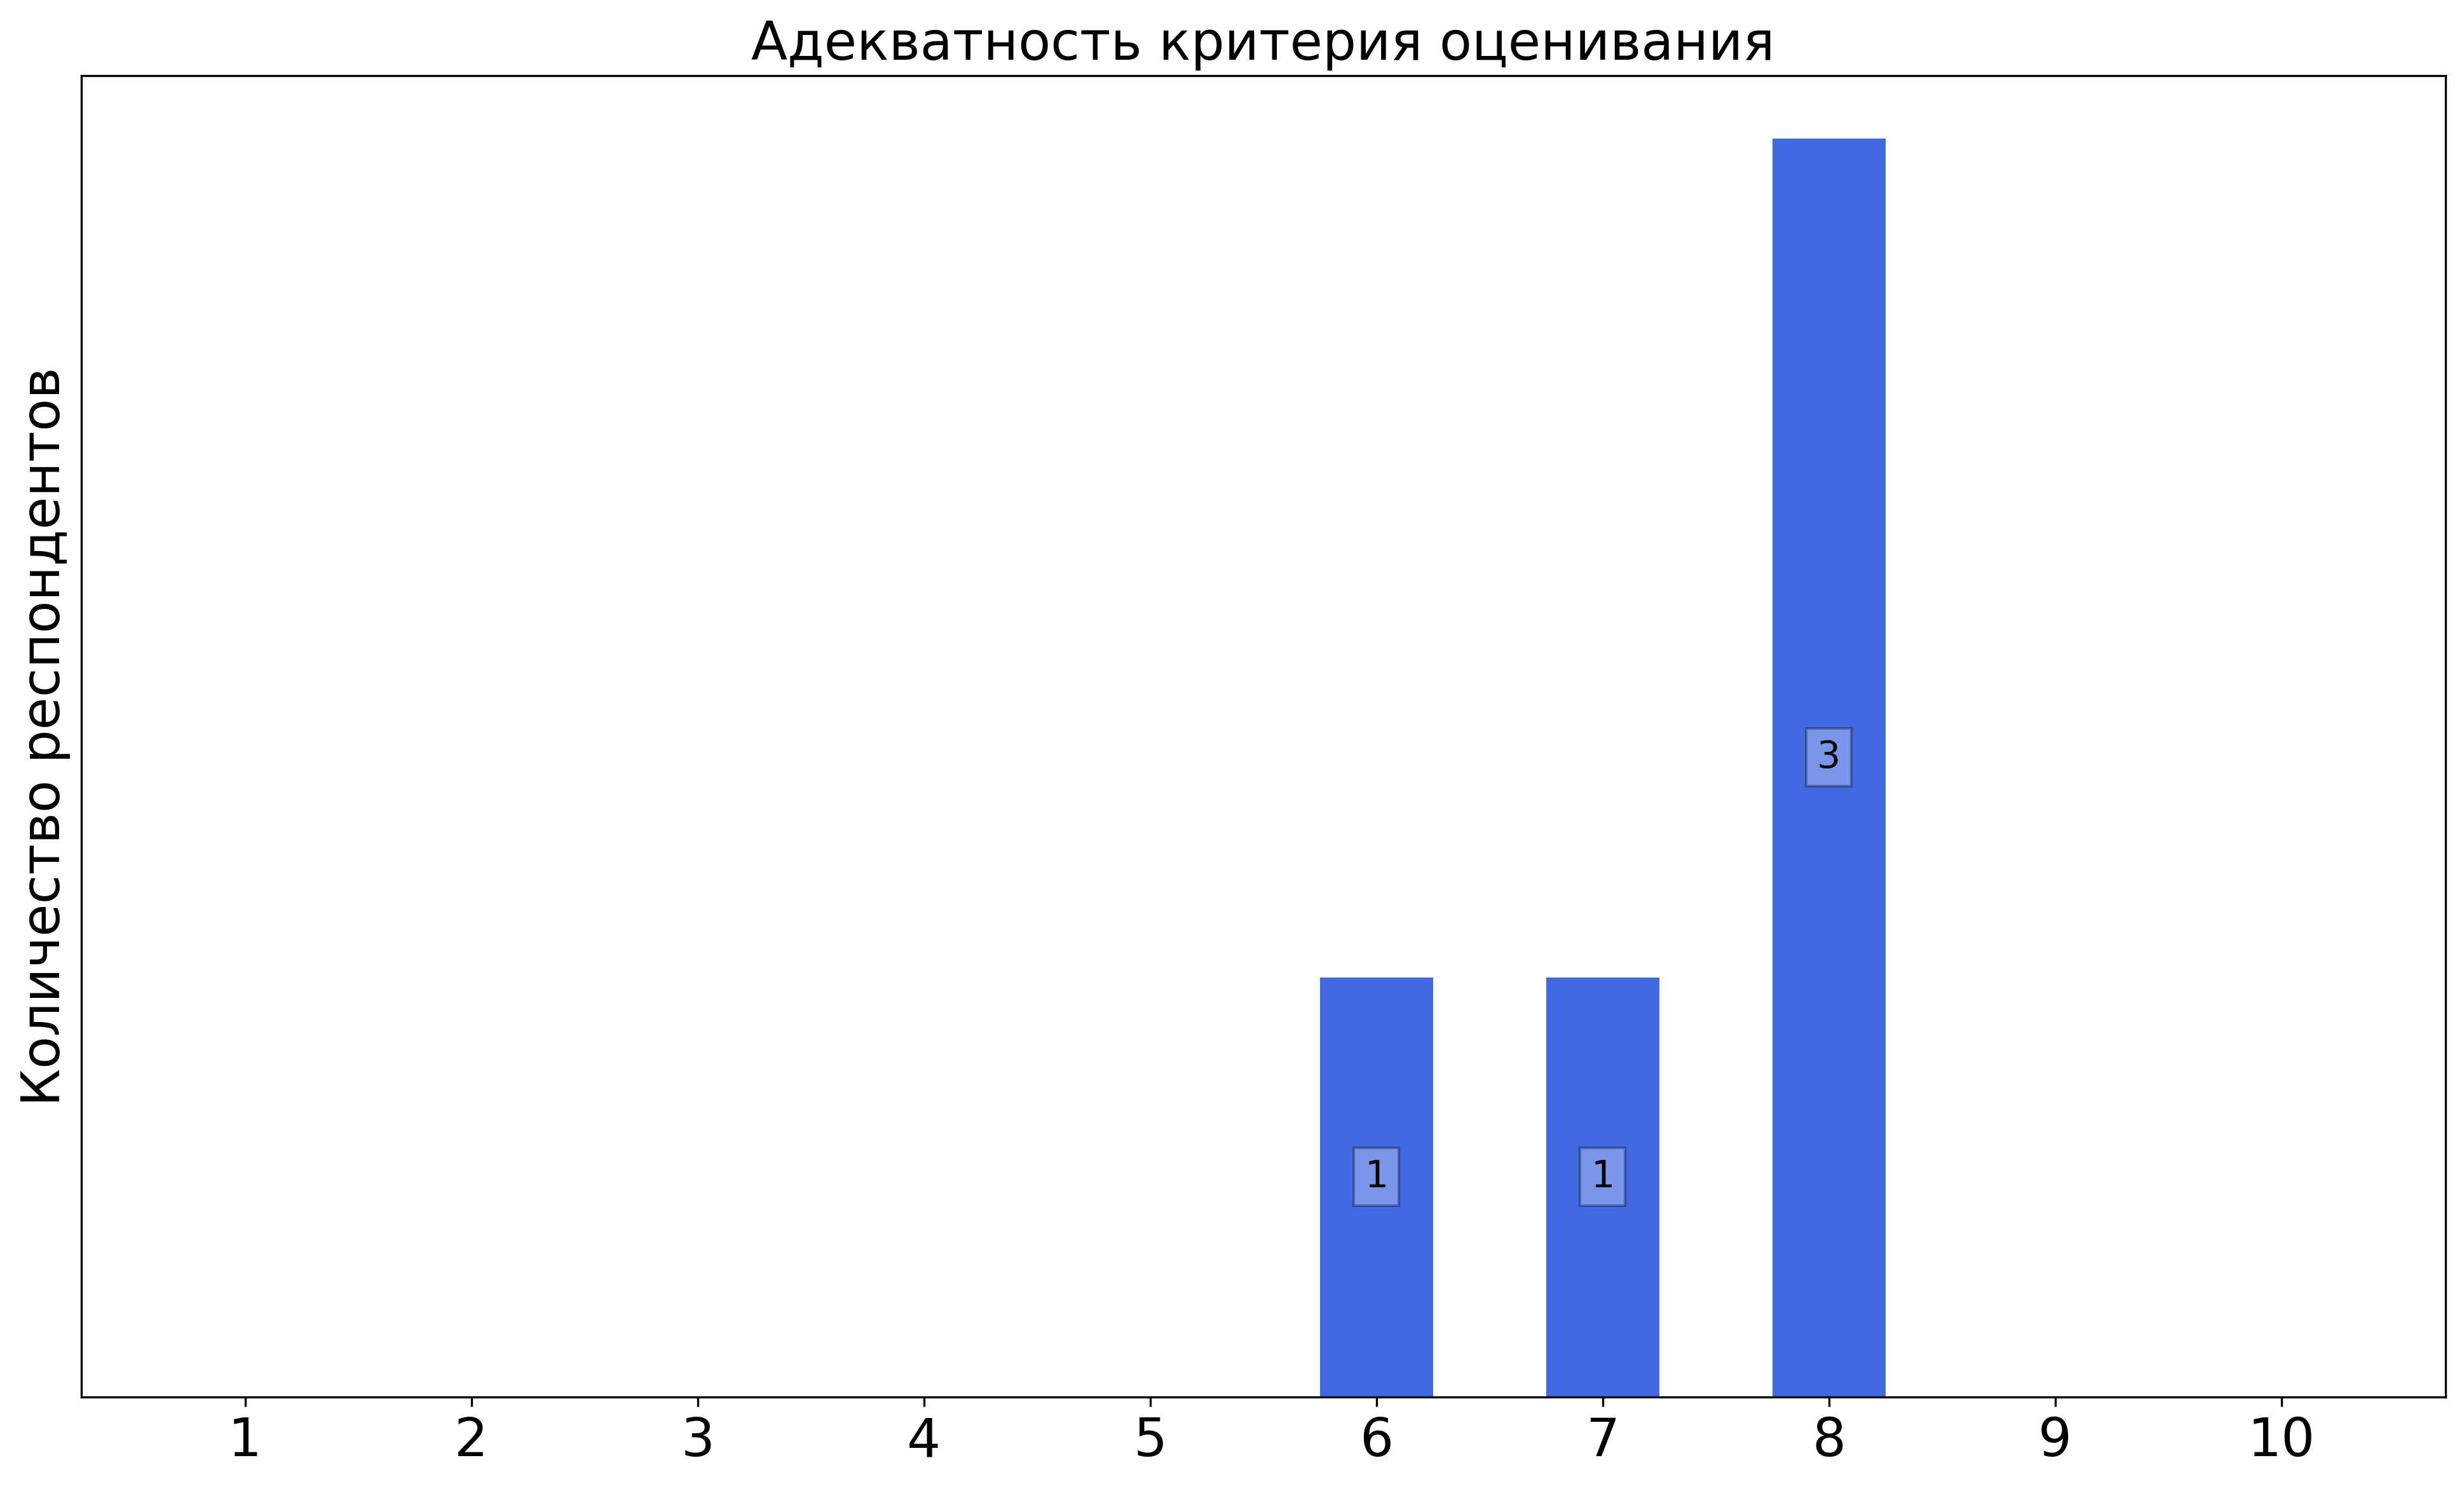
\includegraphics[width=\textwidth]{images/3 course/Аналоговая электроника/labniks-marks-Арумов Г.П.-1.png}
			\end{subfigure}
			\begin{subfigure}[b]{0.45\textwidth}
				\centering
				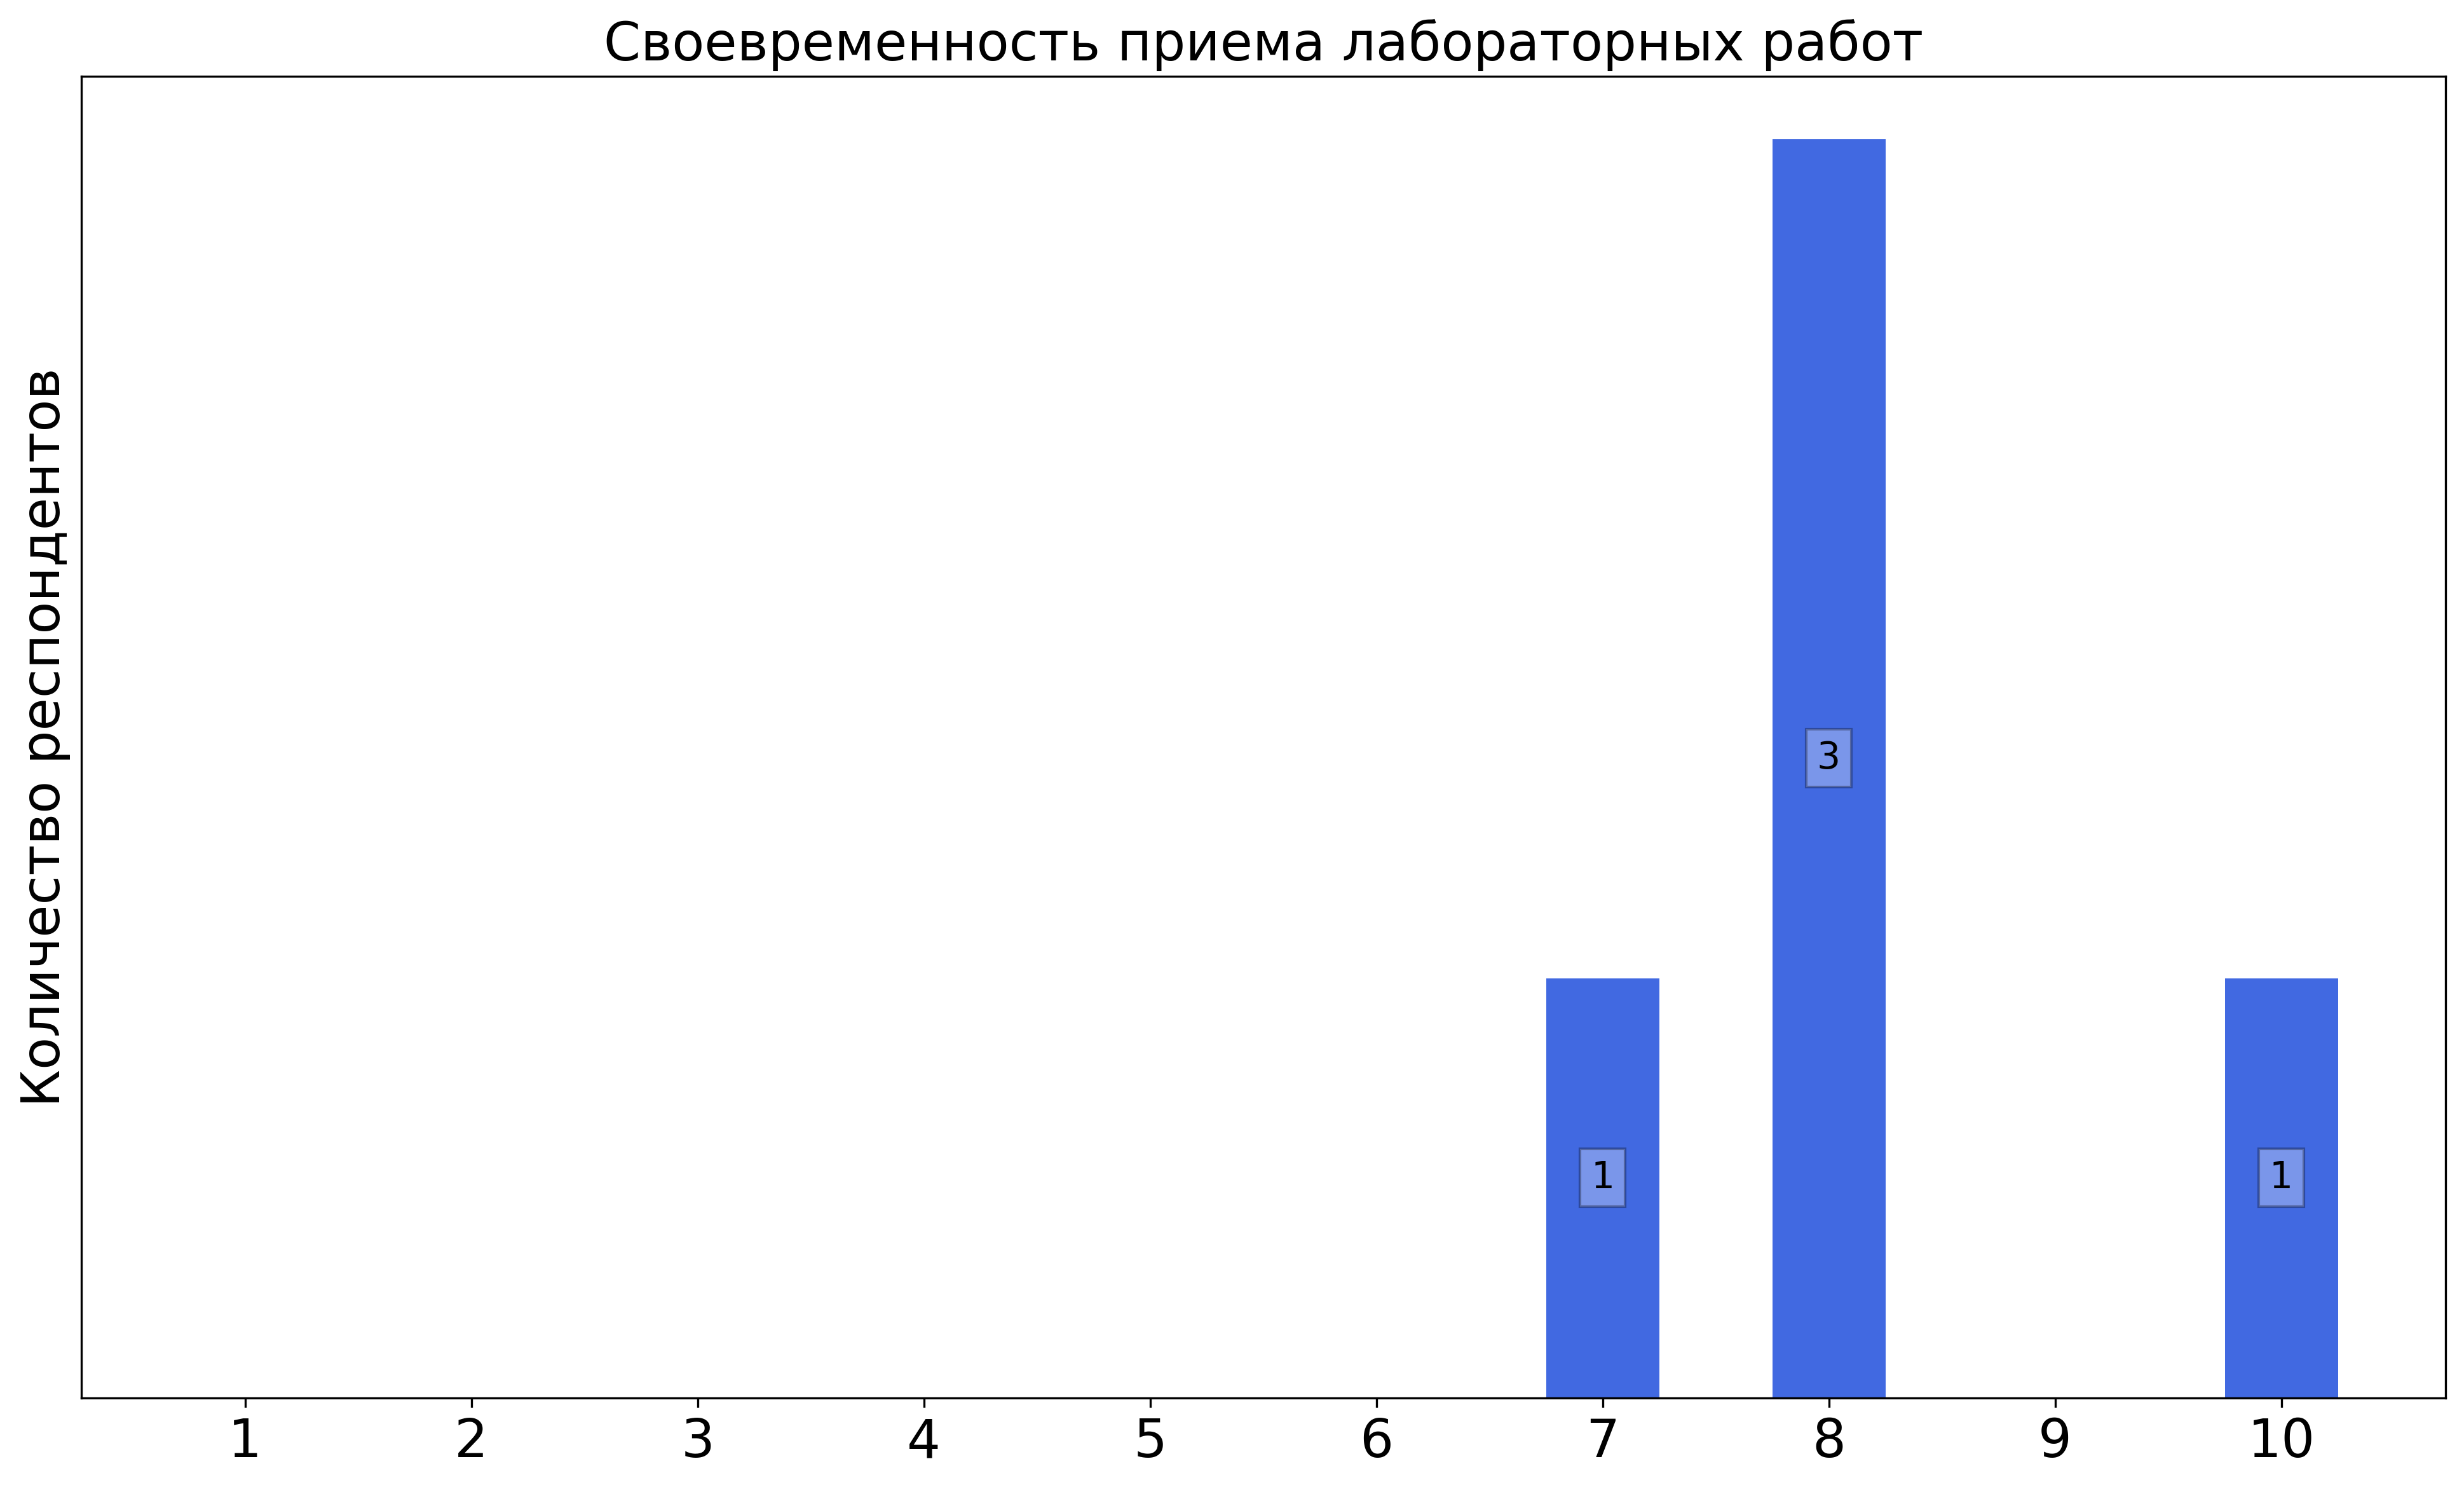
\includegraphics[width=\textwidth]{images/3 course/Аналоговая электроника/labniks-marks-Арумов Г.П.-2.png}
			\end{subfigure}
			\begin{subfigure}[b]{0.45\textwidth}
				\centering
				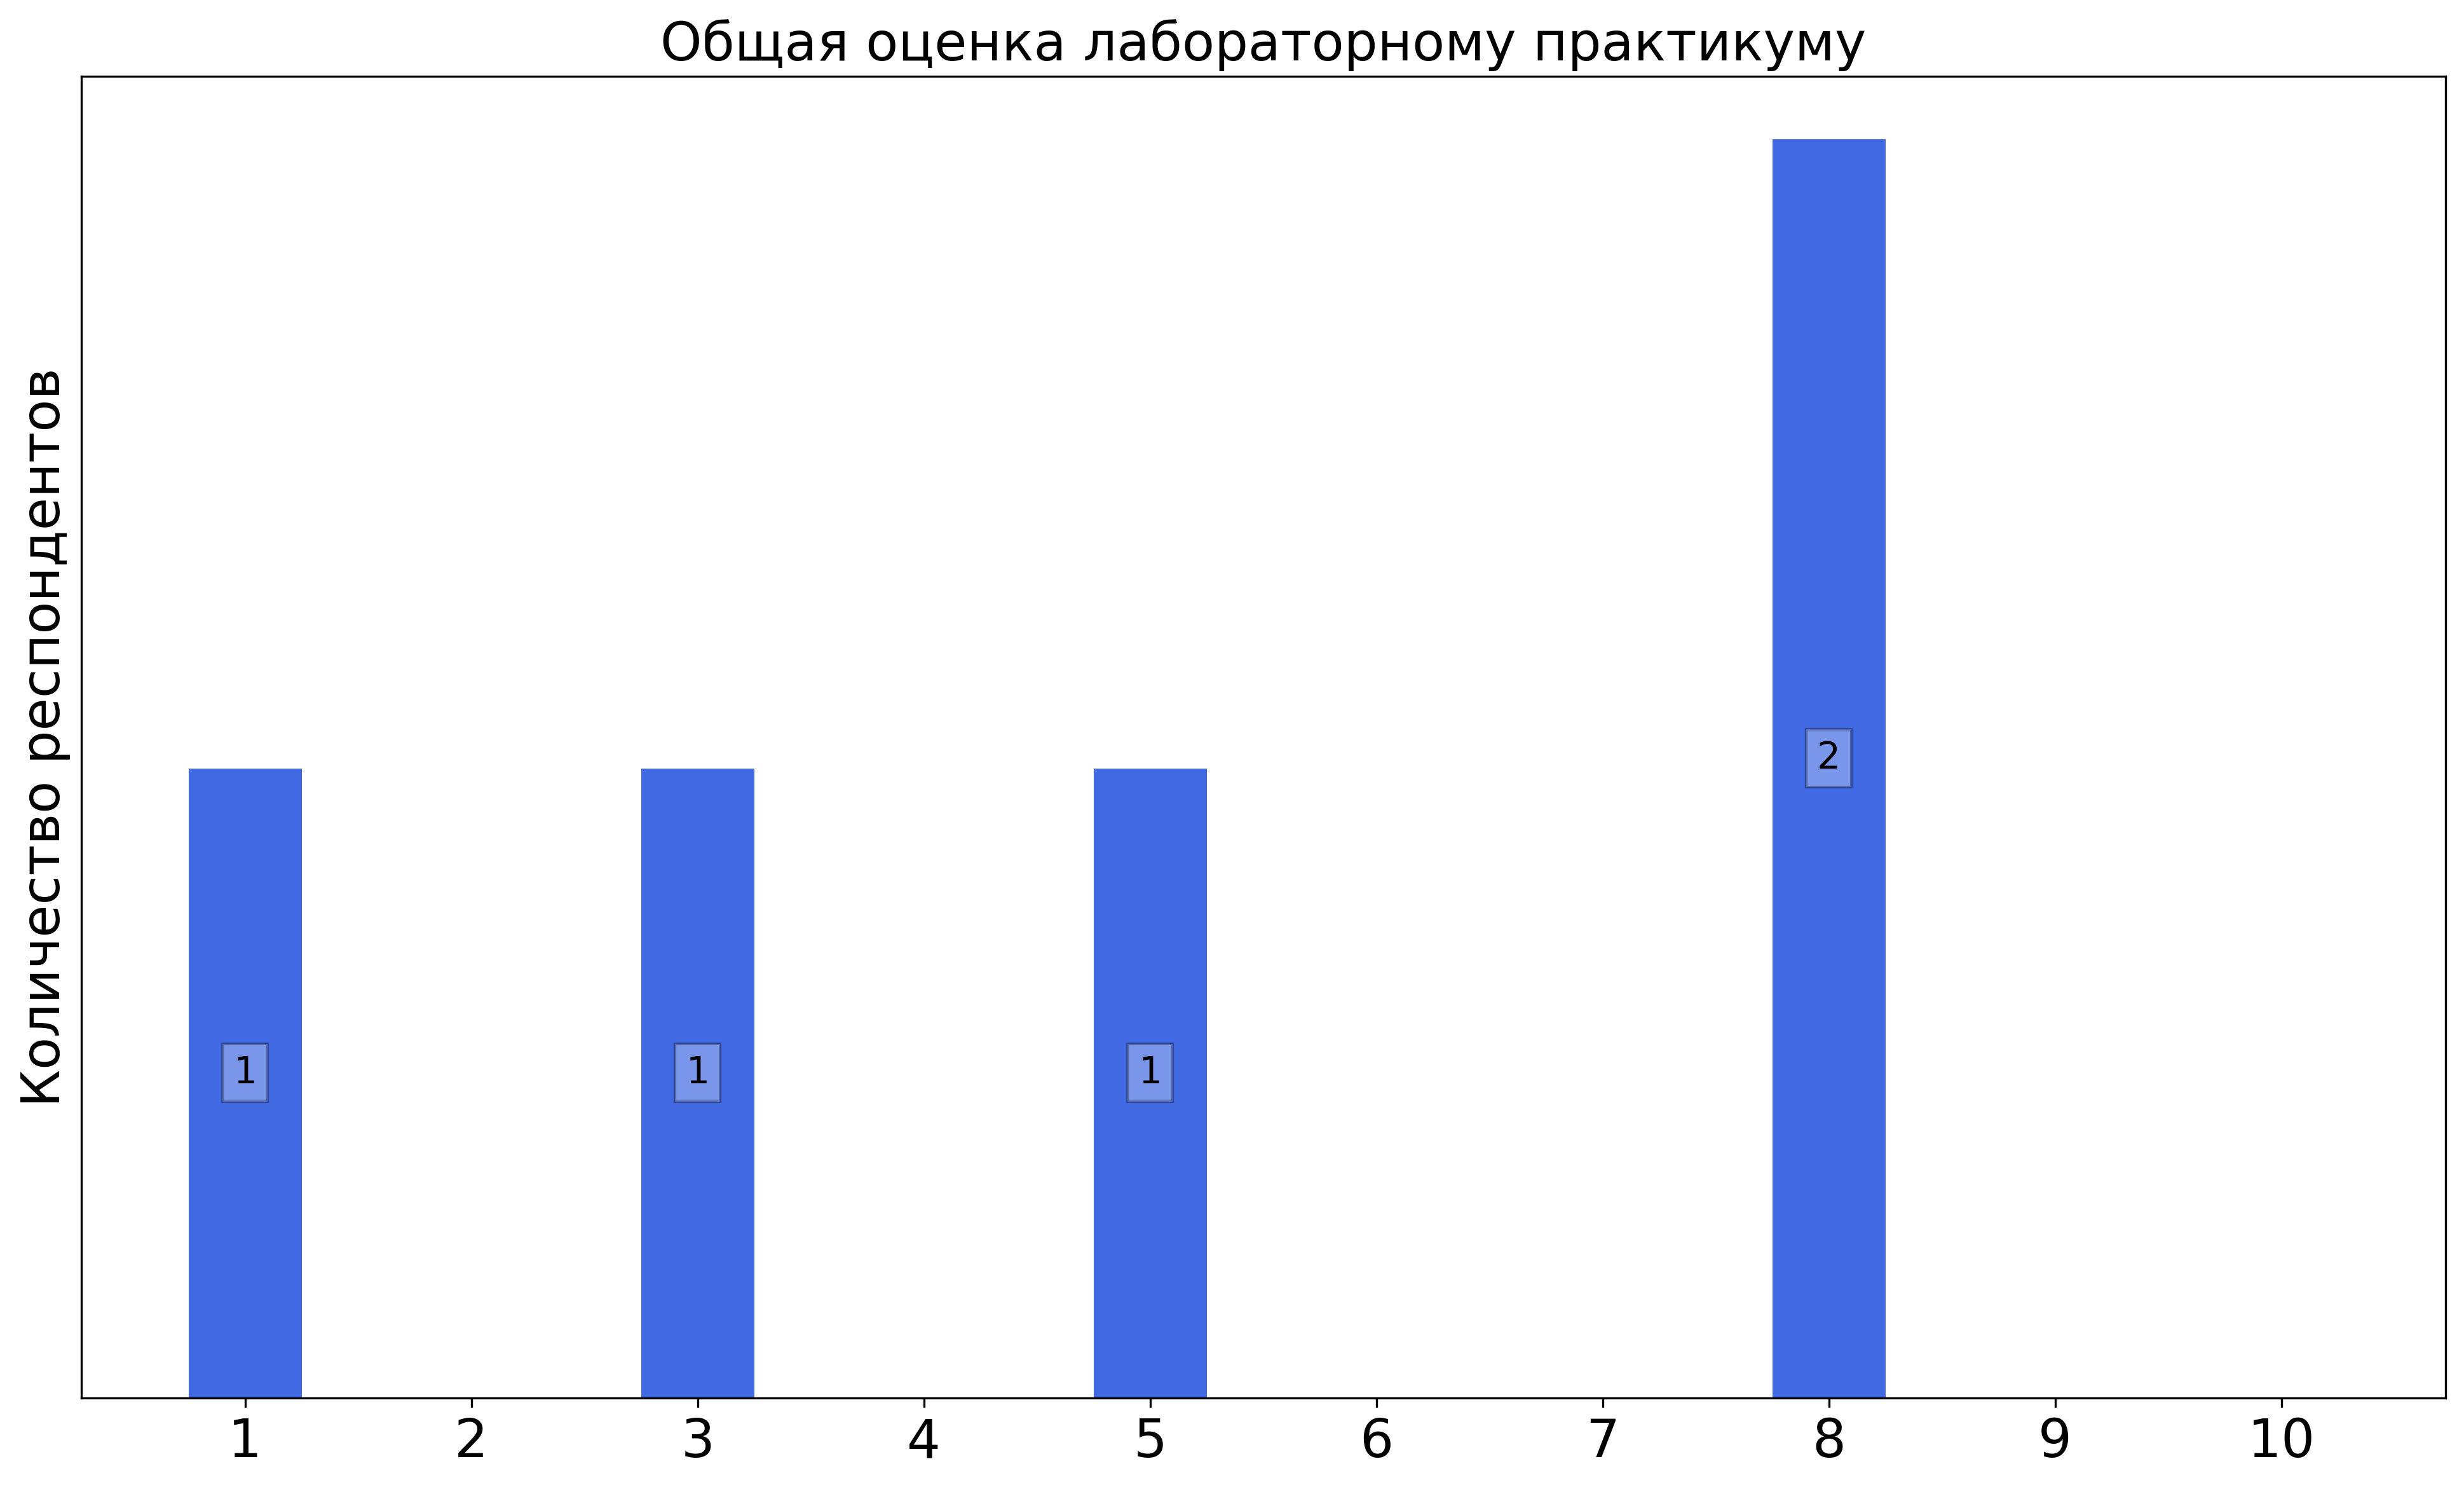
\includegraphics[width=\textwidth]{images/3 course/Аналоговая электроника/labniks-marks-Арумов Г.П.-3.png}
			\end{subfigure}	
			\caption{Оценки респондентов о качестве преподавания лабораторных работ}
		\end{figure}

		\textbf{Комментарии студентов о преподавателе\protect\footnote{сохранены оригинальные орфография и пунктуация}}
            \begin{commentbox} 
                Предмет давно уже не тот. Надо что-то делать, пока всё совсем не умерло 
            \end{commentbox} 
        
            \begin{commentbox} 
                Нехватка компонентов, ломающиеся приборы, устаревшая программа, о чём говорят сами преподаватели.  
            \end{commentbox} 


    \subsubsection{Отзыв студентов о лабораторных работах. Преподаватель: Бибиков А.М.}
		\begin{figure}[H]
			\centering
			\begin{subfigure}[b]{0.45\textwidth}
				\centering
				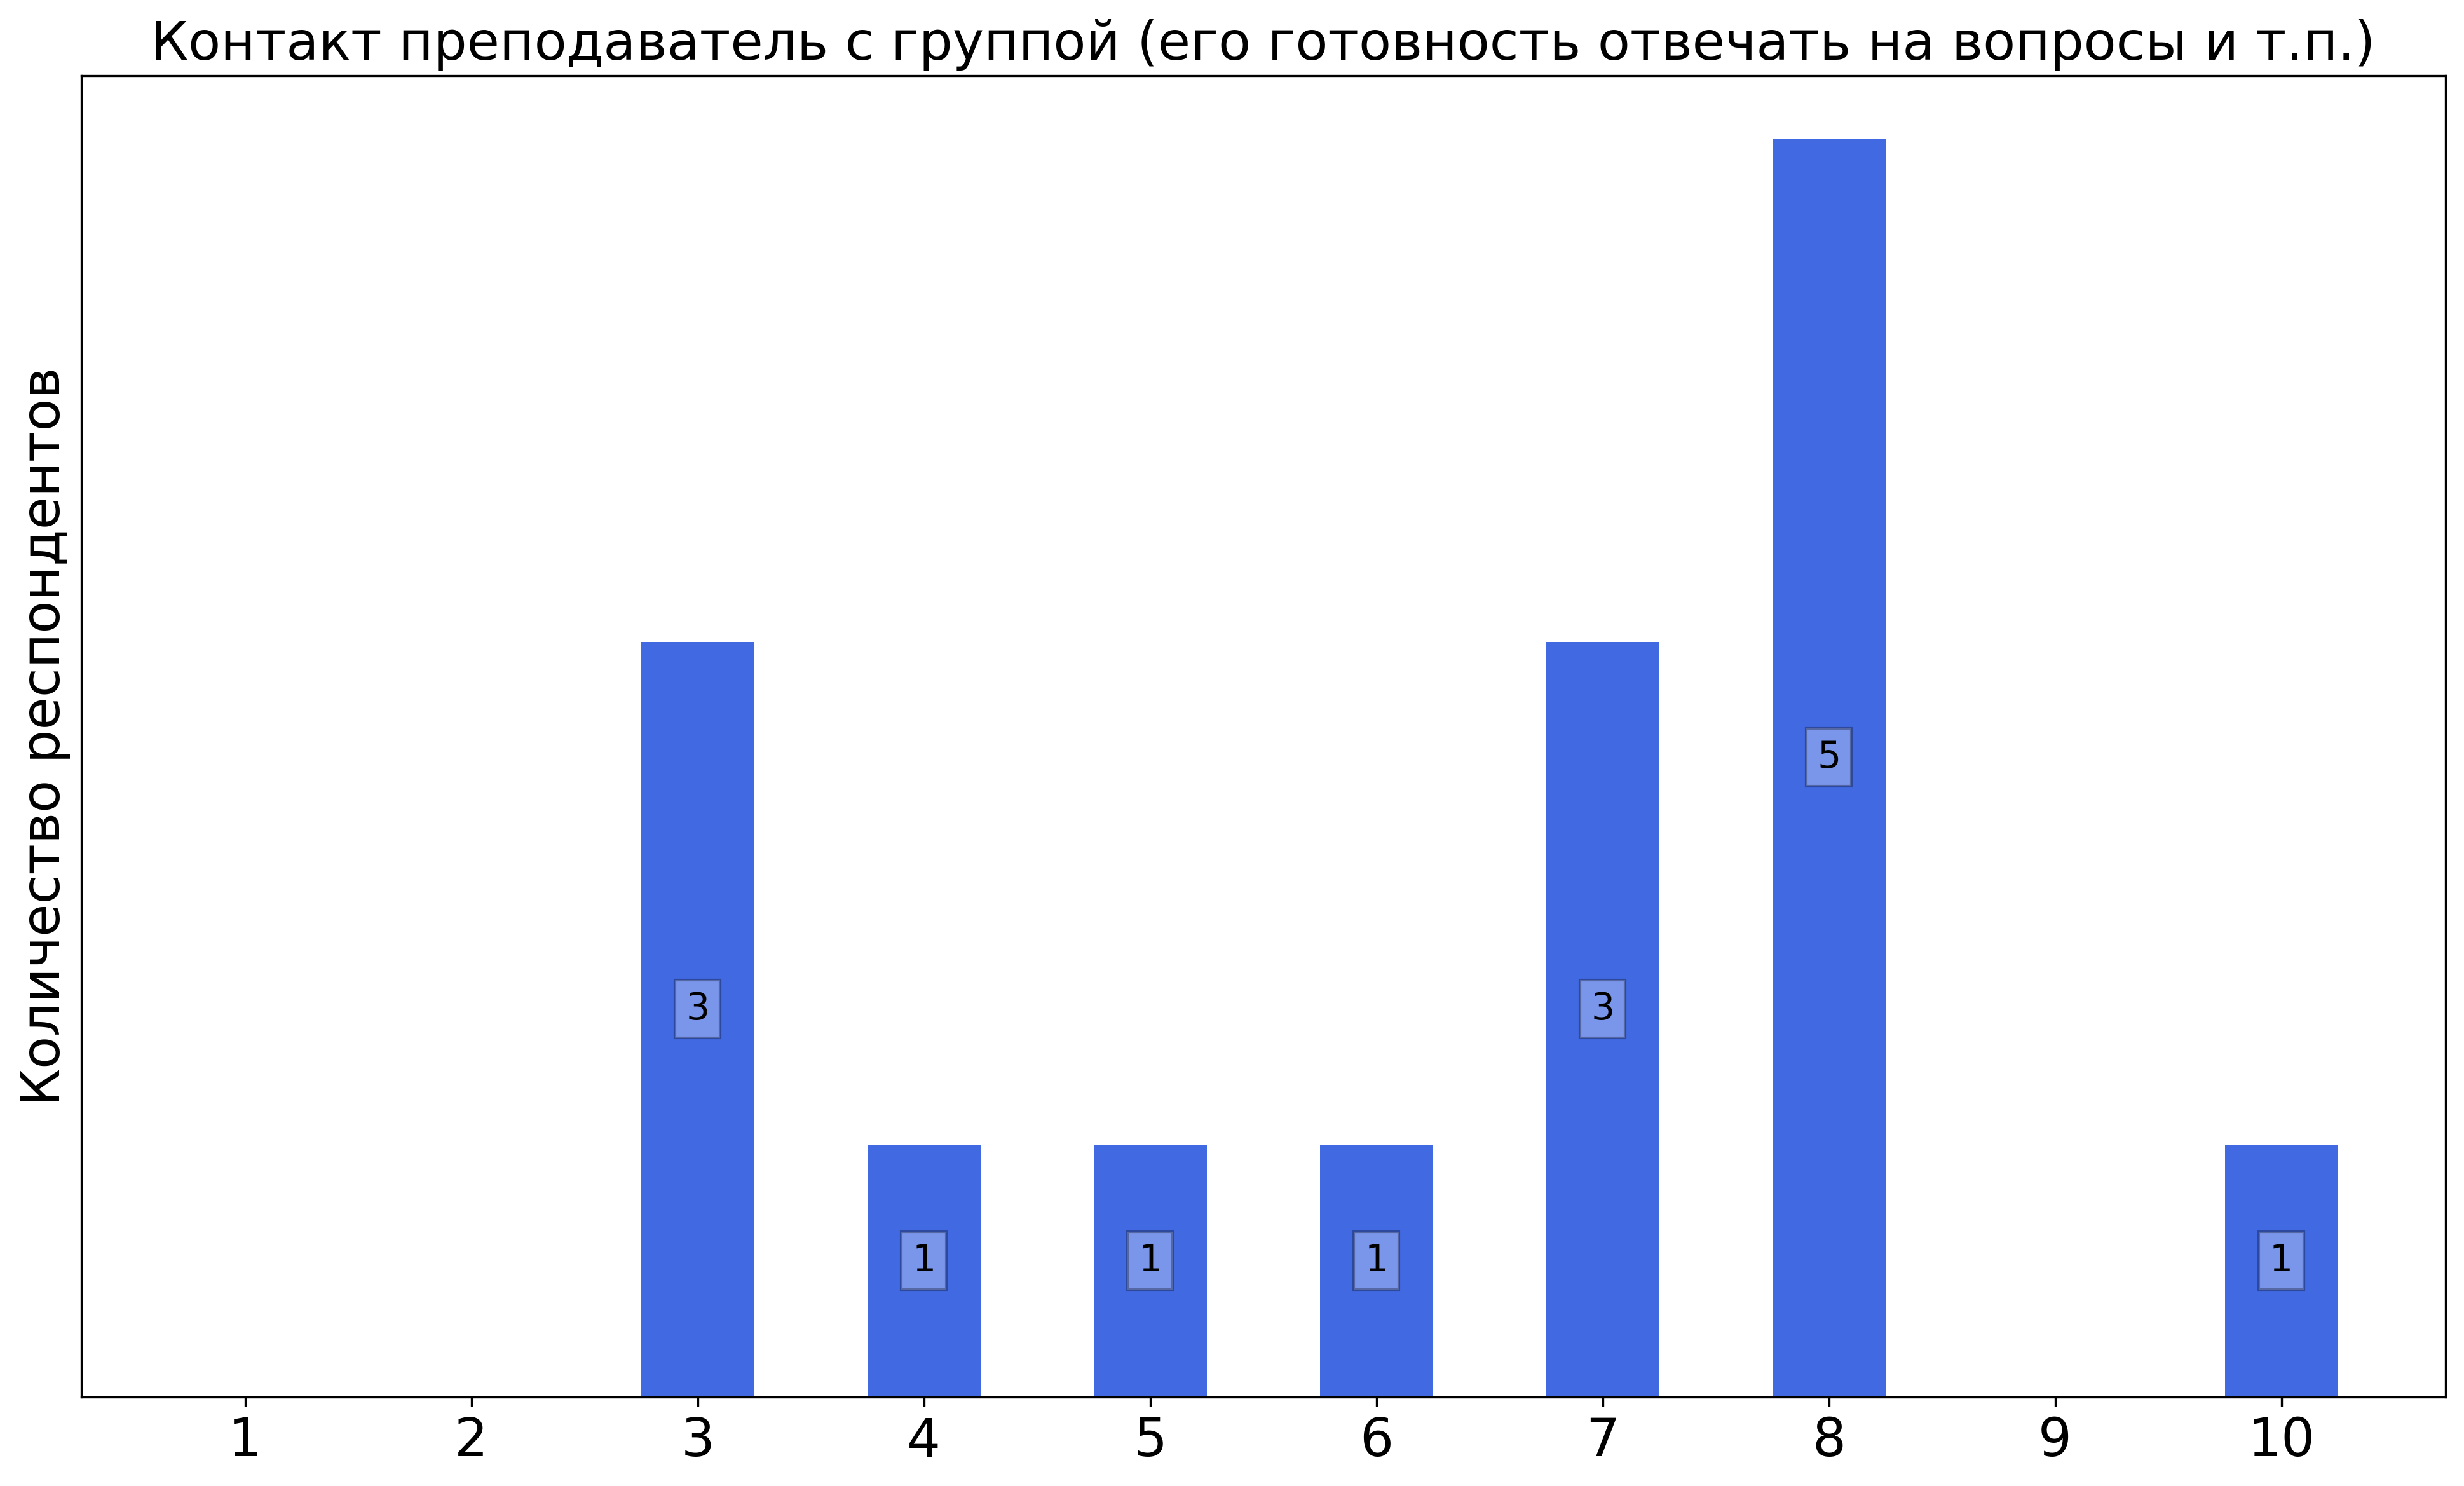
\includegraphics[width=\textwidth]{images/3 course/Аналоговая электроника/labniks-marks-Бибиков А.М.-0.png}
			\end{subfigure}
			\begin{subfigure}[b]{0.45\textwidth}
				\centering
				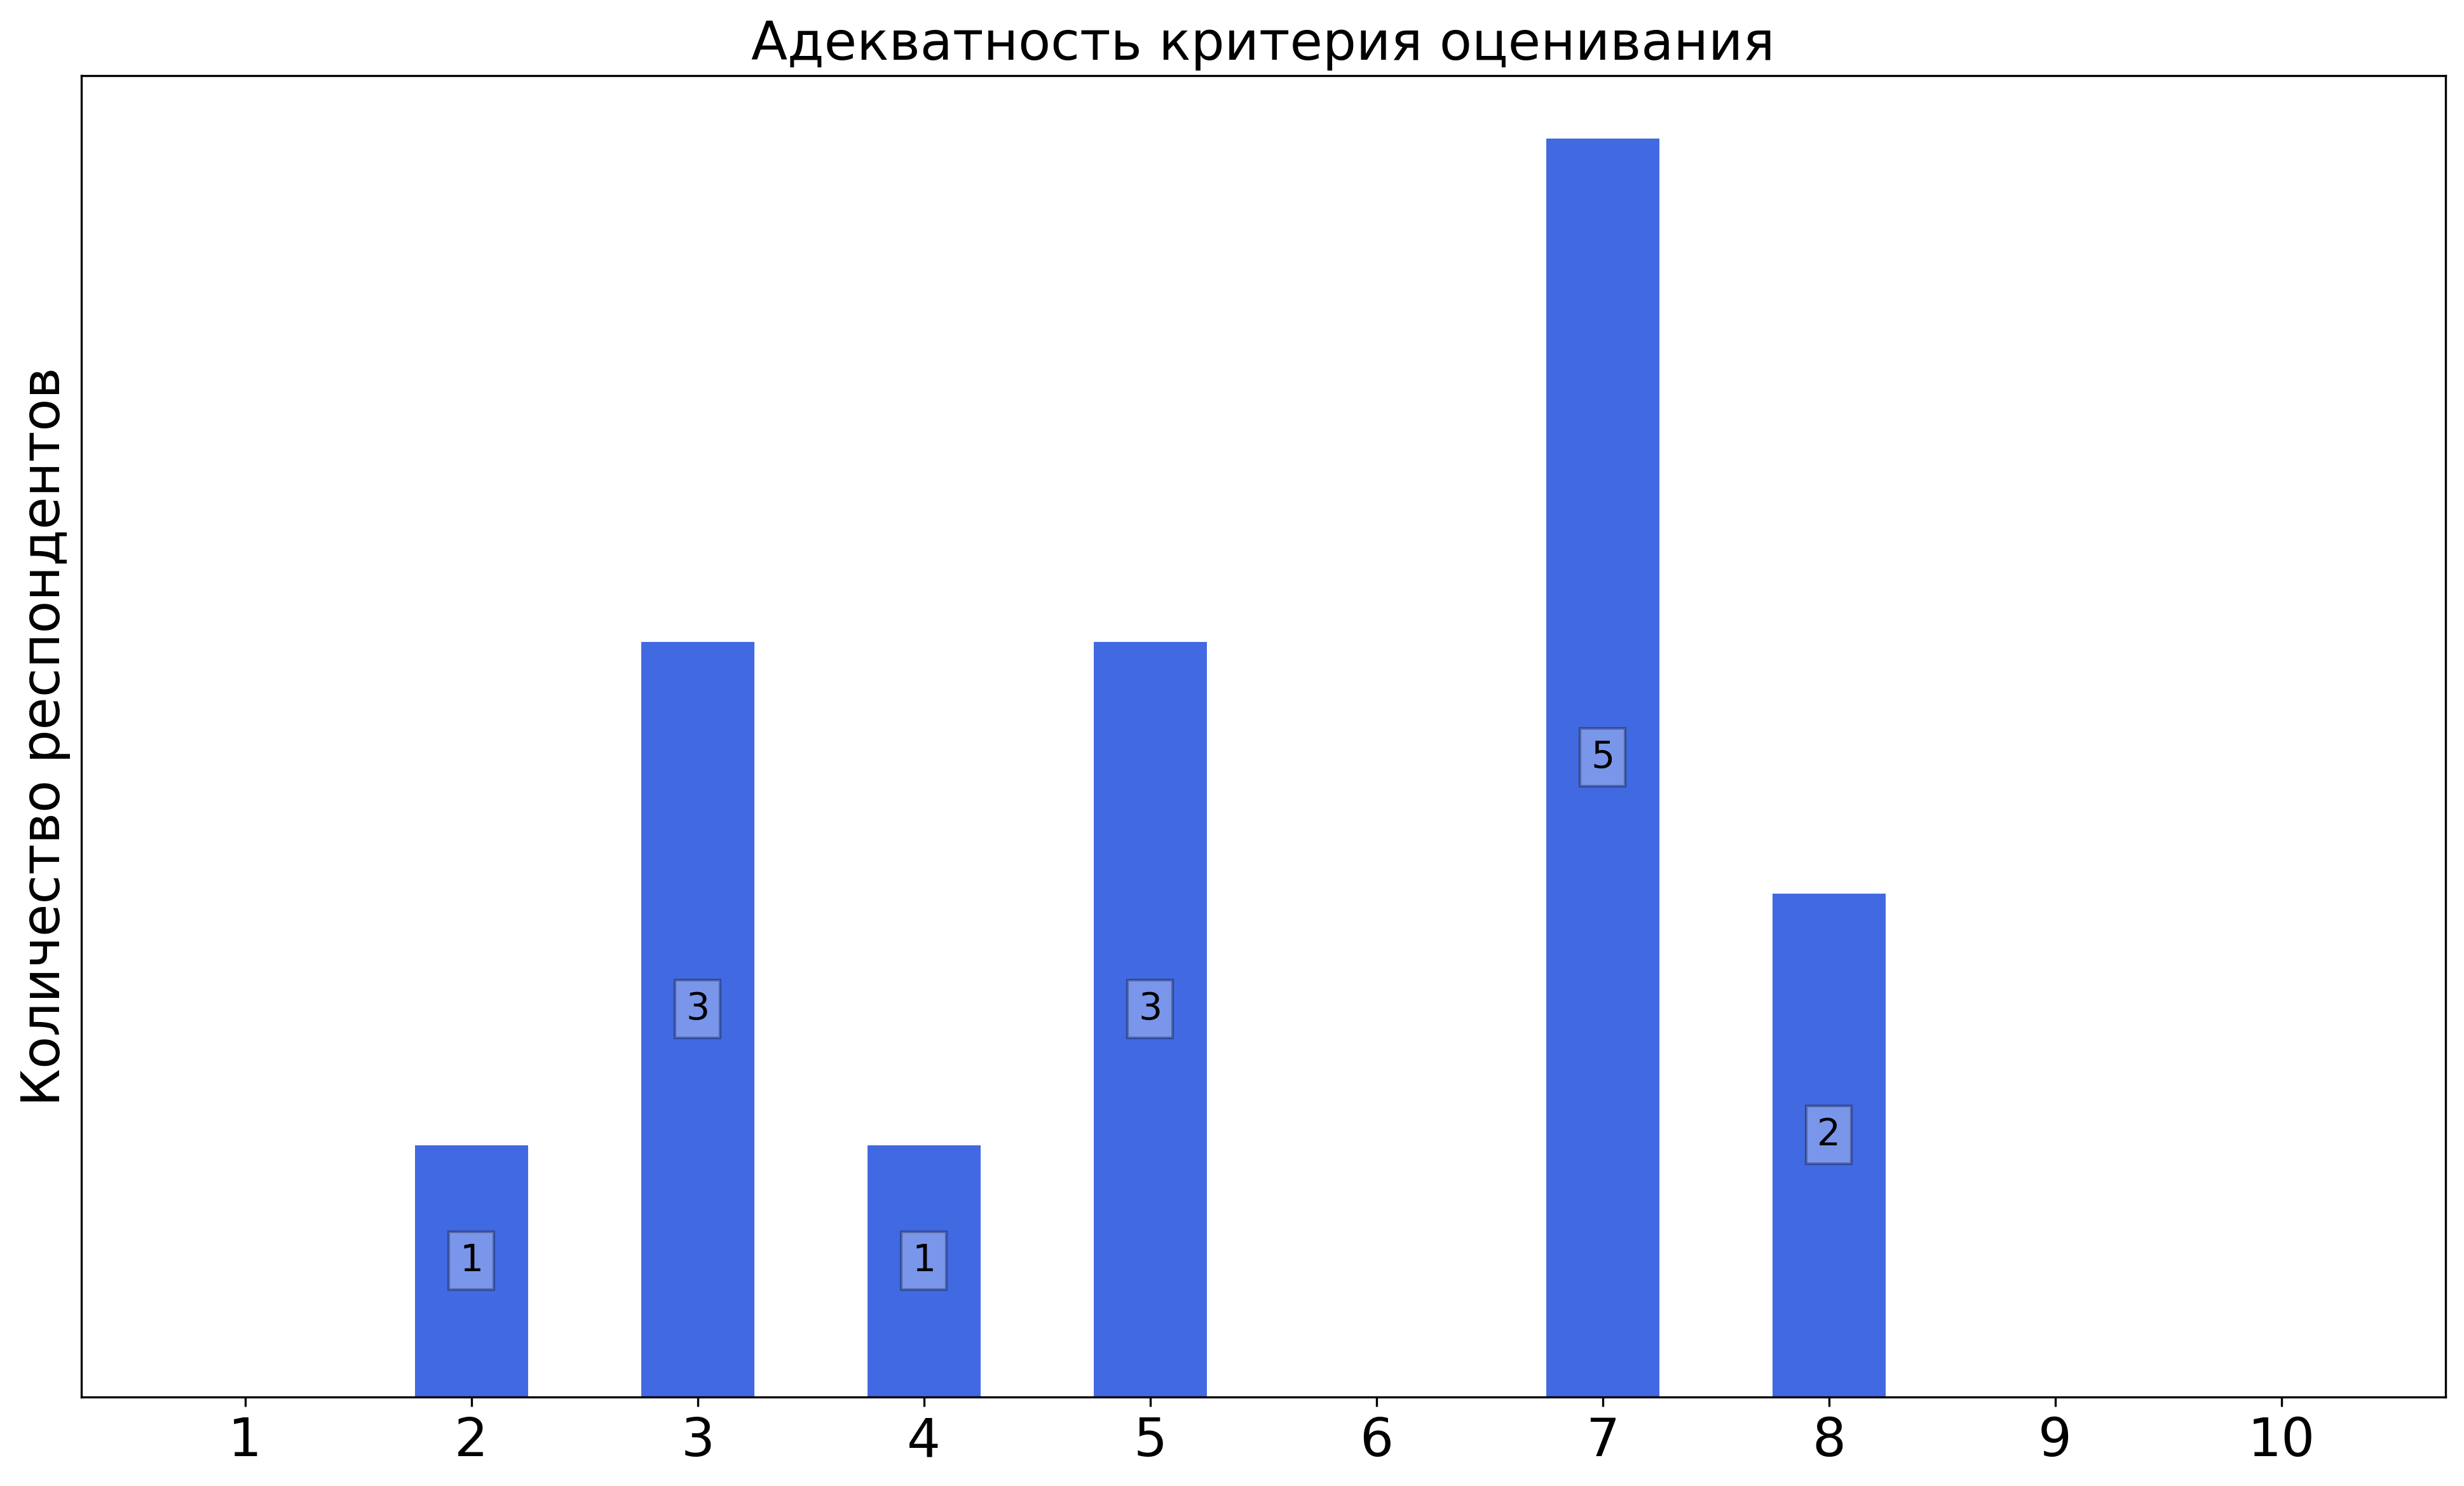
\includegraphics[width=\textwidth]{images/3 course/Аналоговая электроника/labniks-marks-Бибиков А.М.-1.png}
			\end{subfigure}
			\begin{subfigure}[b]{0.45\textwidth}
				\centering
				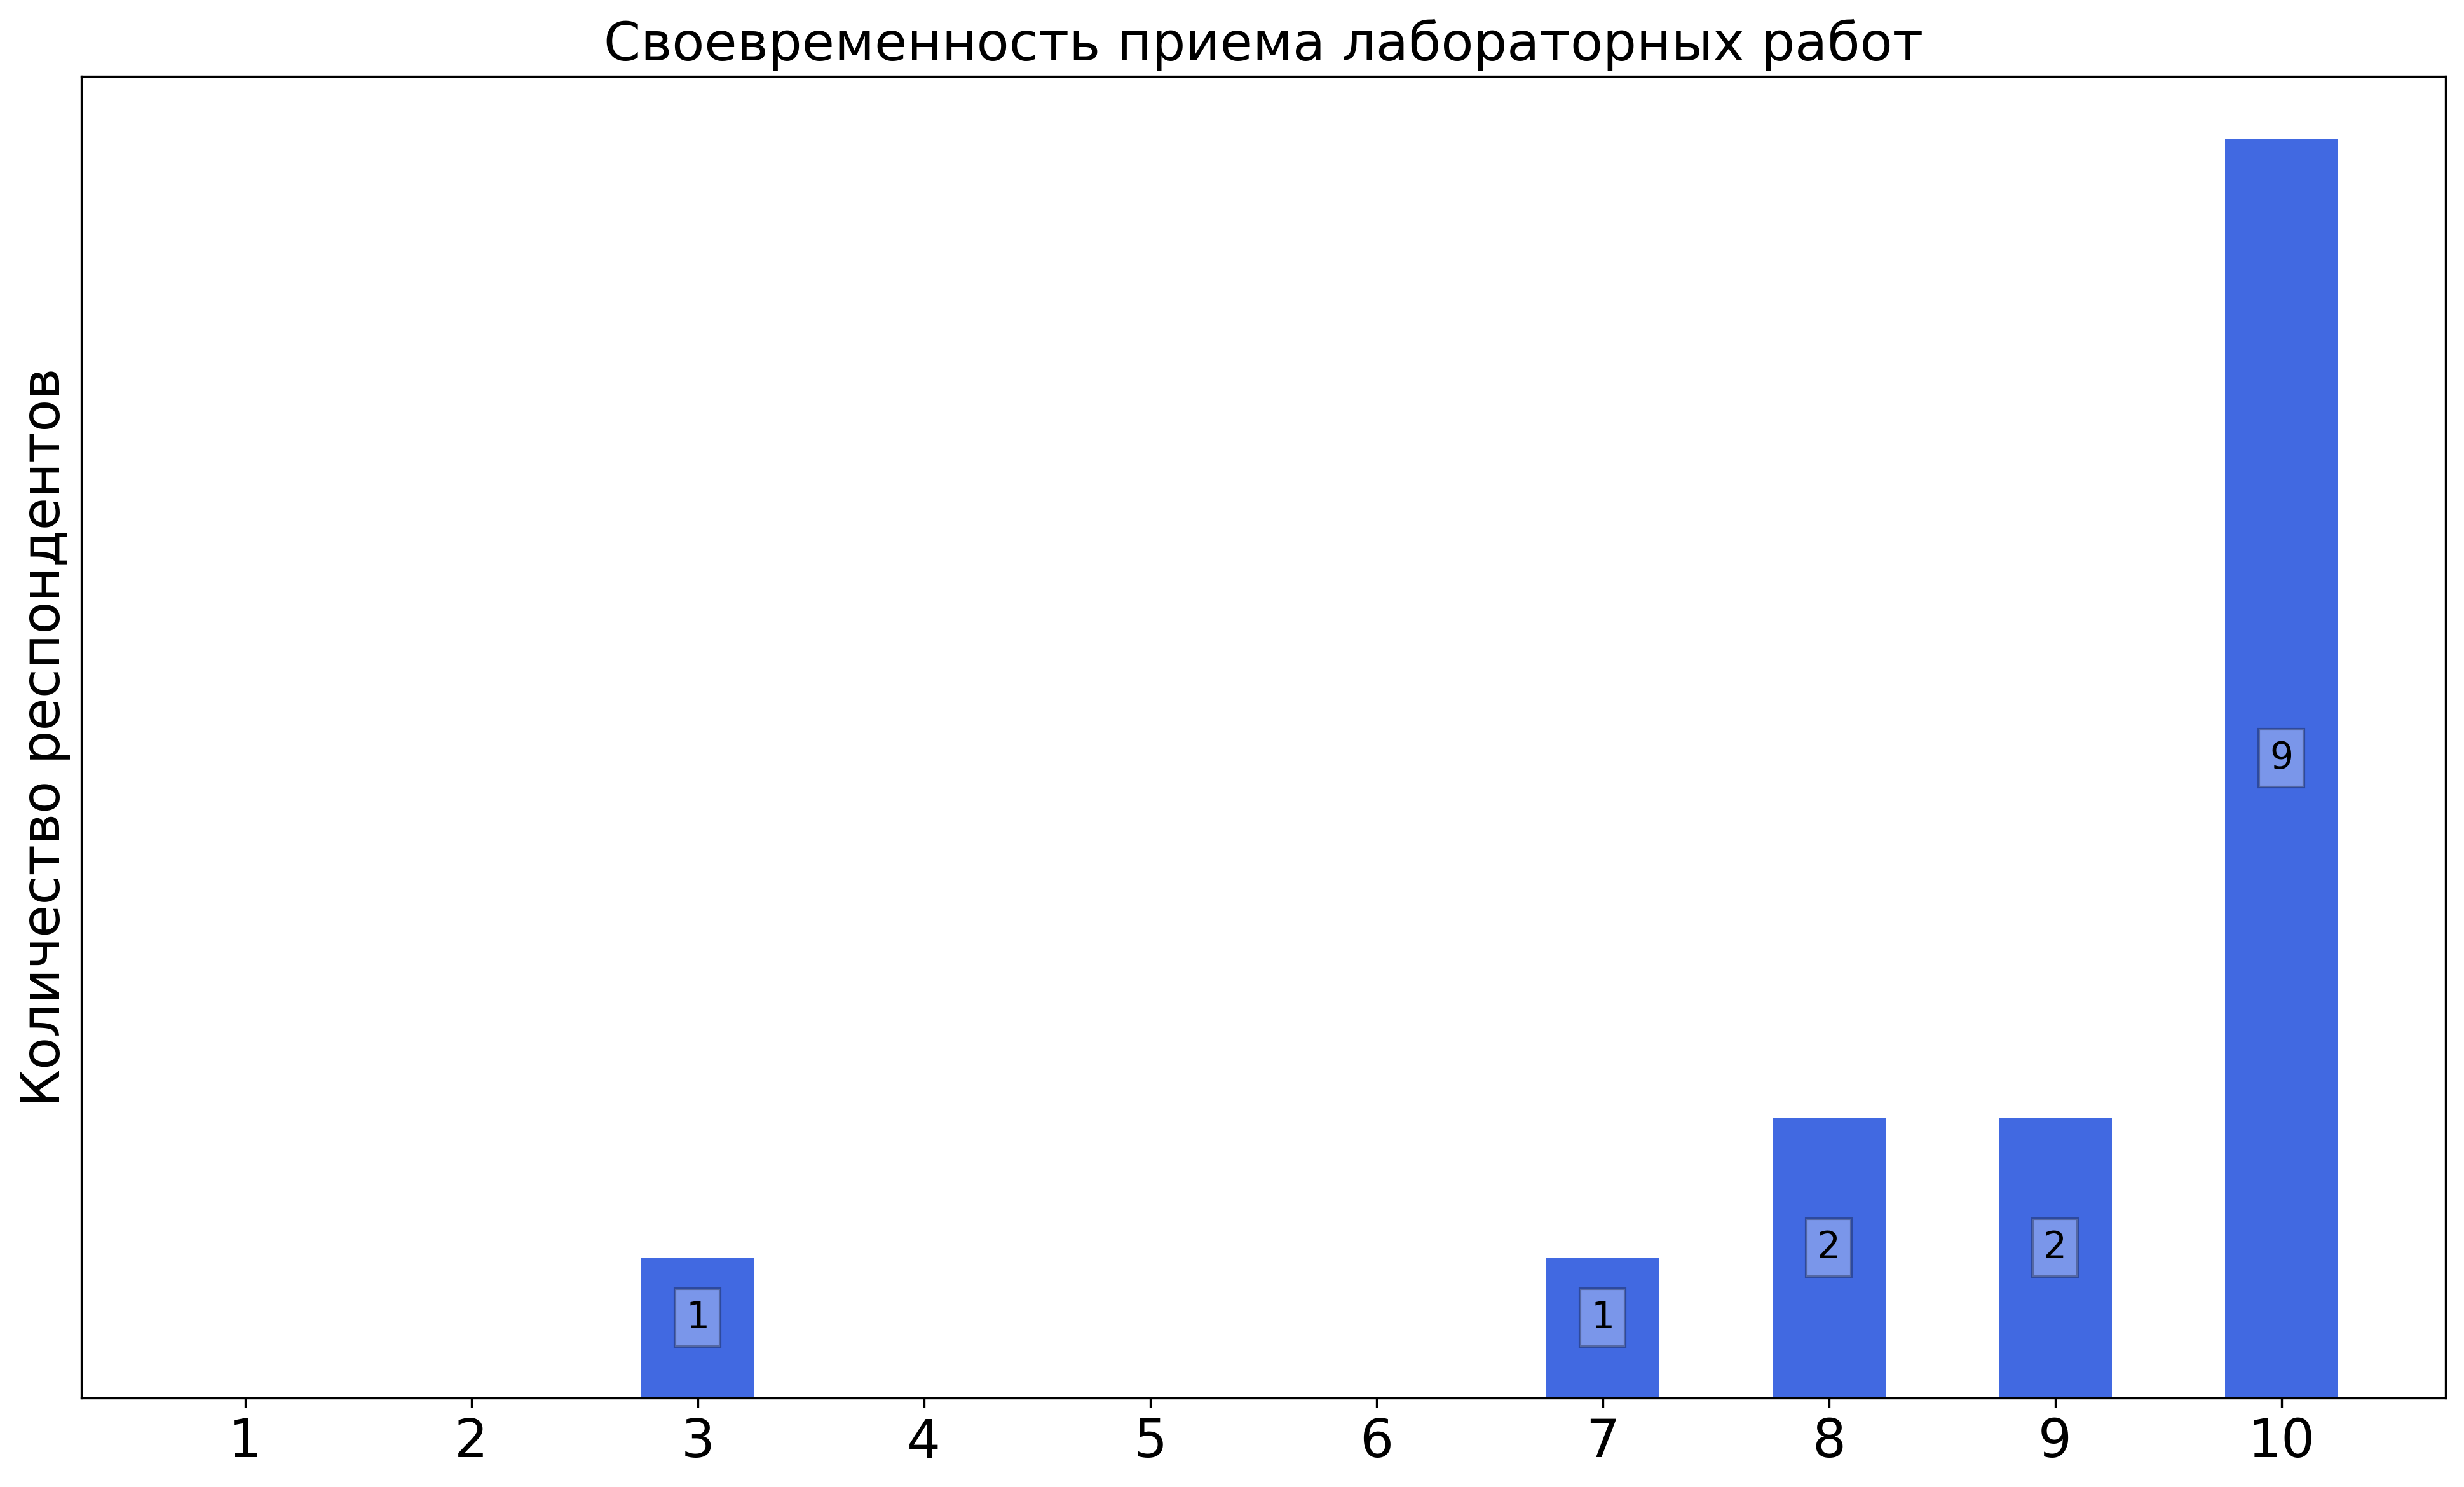
\includegraphics[width=\textwidth]{images/3 course/Аналоговая электроника/labniks-marks-Бибиков А.М.-2.png}
			\end{subfigure}
			\begin{subfigure}[b]{0.45\textwidth}
				\centering
				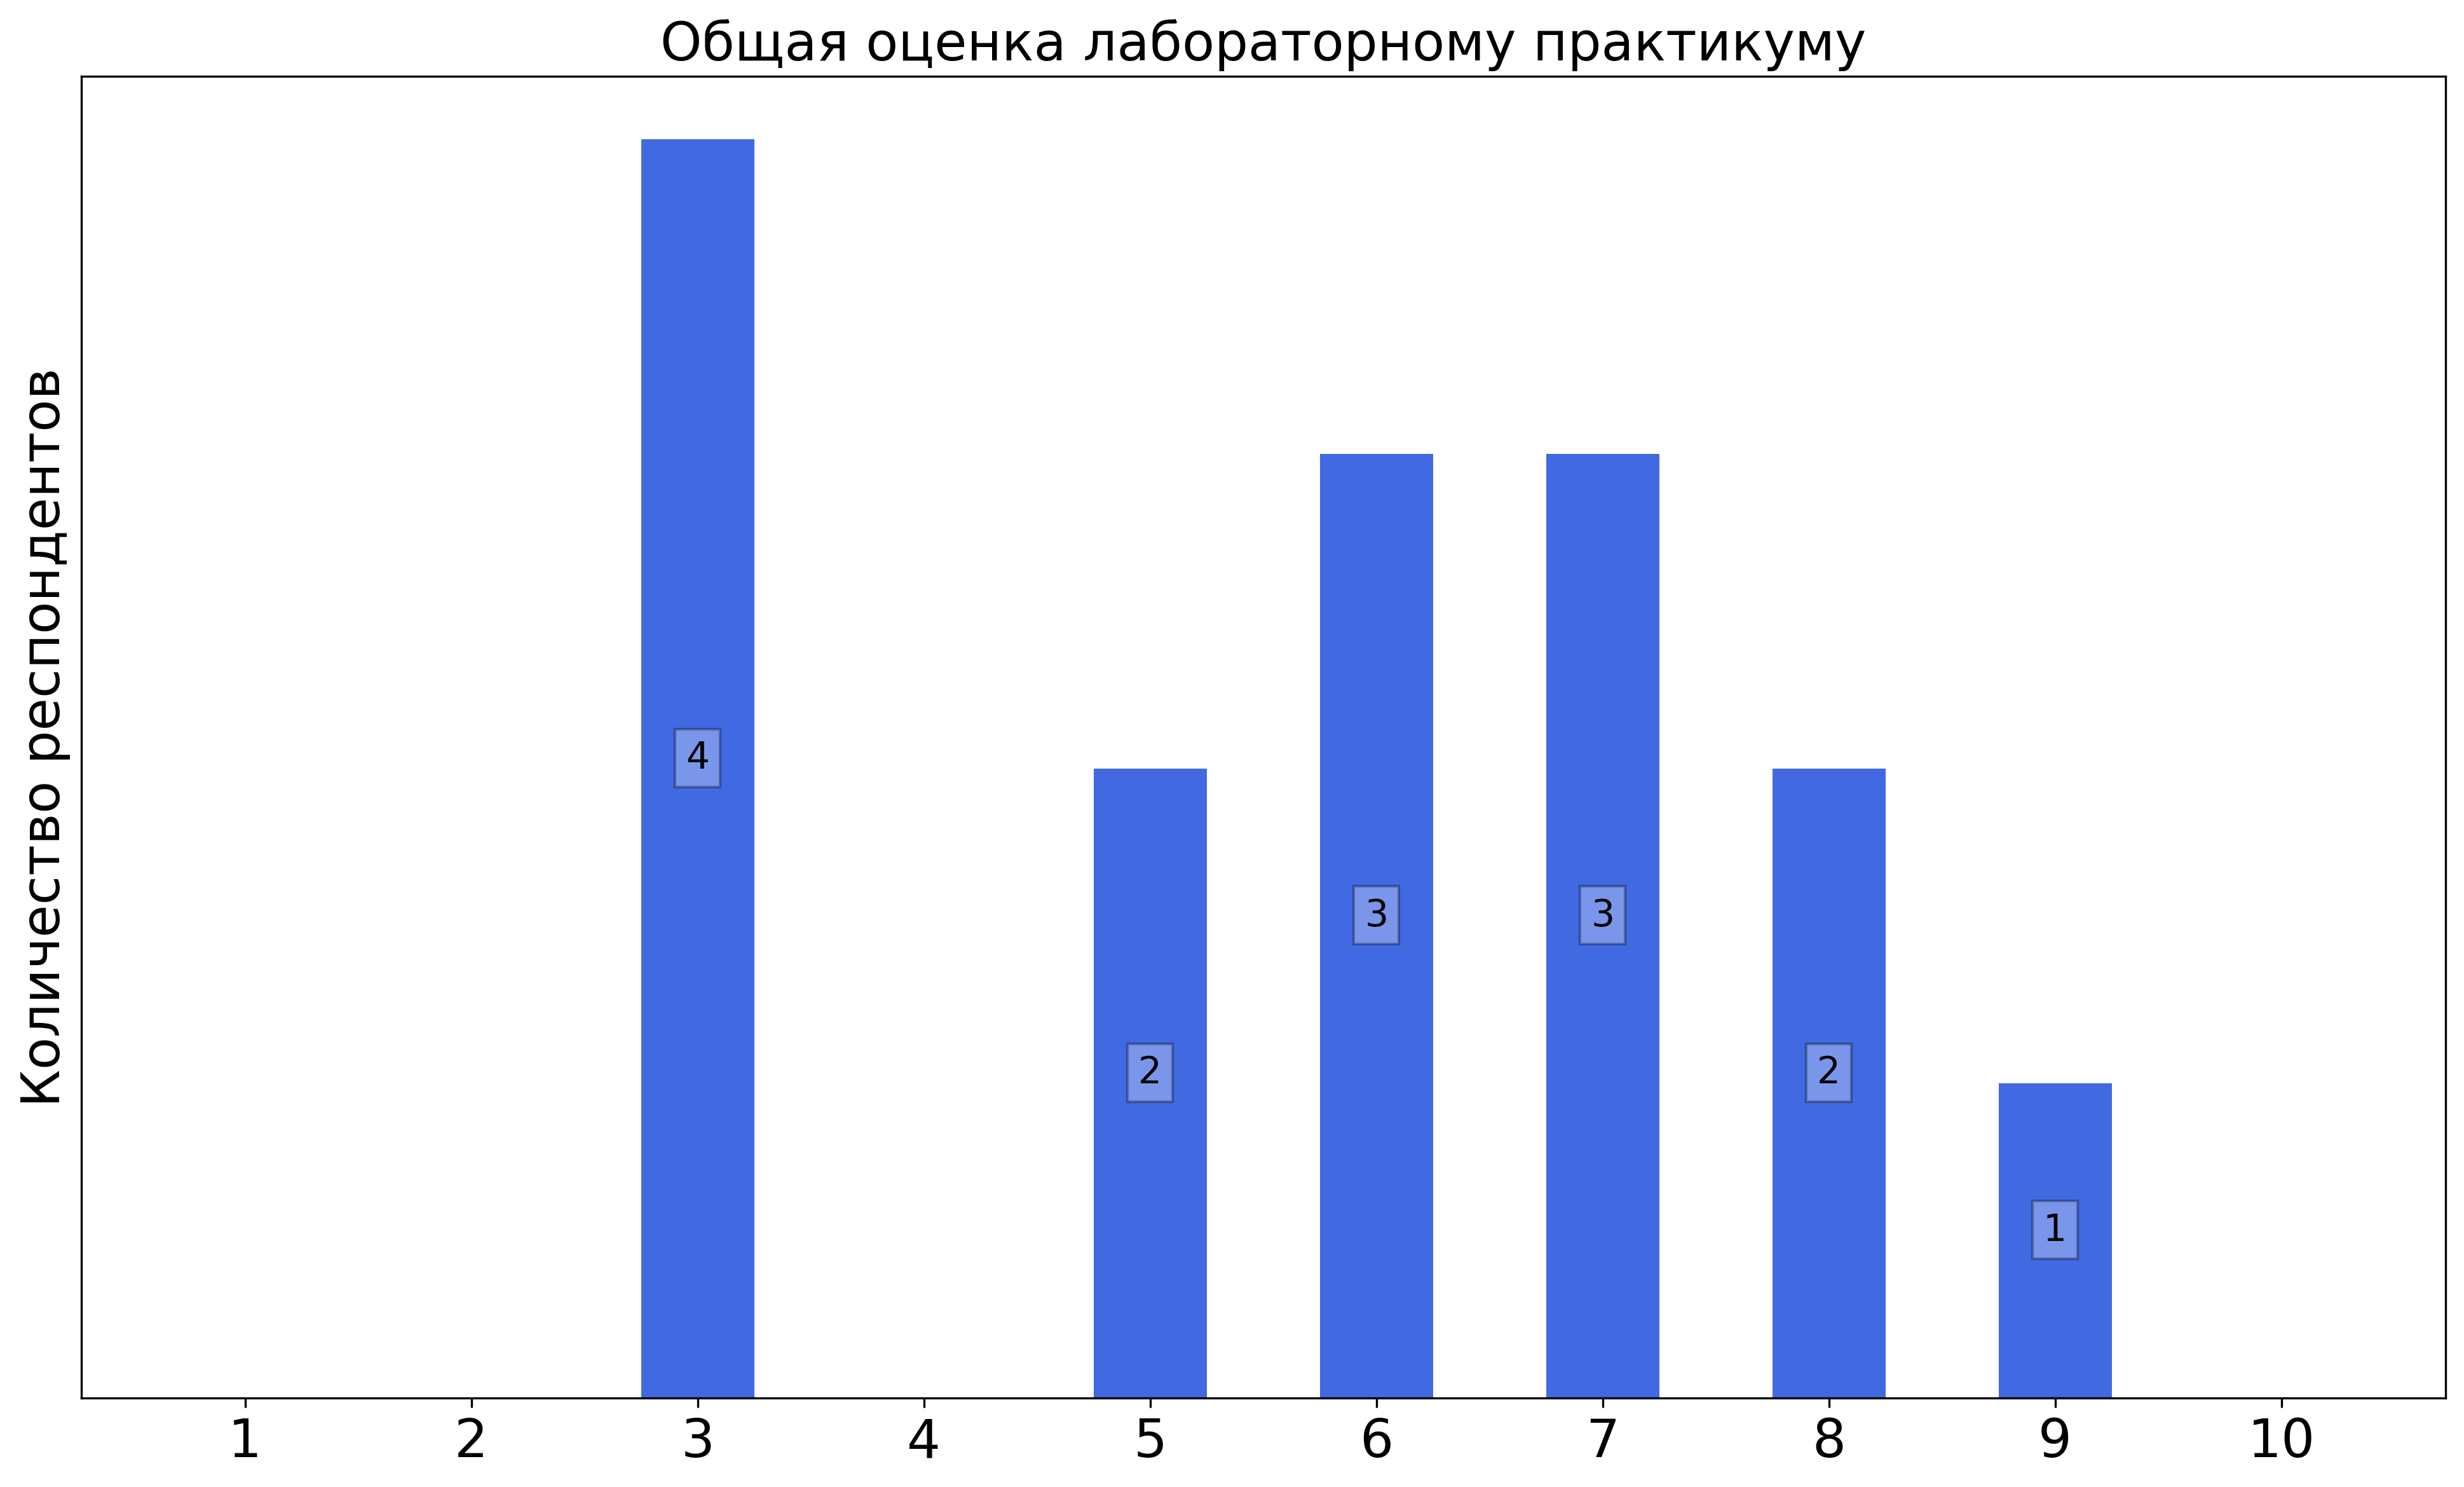
\includegraphics[width=\textwidth]{images/3 course/Аналоговая электроника/labniks-marks-Бибиков А.М.-3.png}
			\end{subfigure}	
			\caption{Оценки респондентов о качестве преподавания лабораторных работ}
		\end{figure}

		\textbf{Комментарии студентов о преподавателе\protect\footnote{сохранены оригинальные орфография и пунктуация}}
            \begin{commentbox} 
                По лабораторным претензий нет  
            \end{commentbox} 
        
            \begin{commentbox} 
                Преподаватель проверяет именно понимание предмета, причем достаточно разносторонне. Надо либо реально все знать, либо попытаться угадать, что от тебя хотят услышать. Оценки выставляются по личному восприятию проведенного диалога, некоторые не очень сдали в начале, и потом никогда не получали выше 7. По-моему, больше 9 не получал никто. Преподаватель обычно не находится в аудитории, но его всегда можно позвать, на все вопросы ответит. 
            \end{commentbox} 
        
            \begin{commentbox} 
                Странное оценивание на семинарах 
            \end{commentbox} 
        
            \begin{commentbox} 
                Преподаватель строго спрашивает, есть некоторые вопросы по критерию выставления оценки. К самому лабораторному курсу вопросов нет, его можно считать эталоном, но желание преподавателя переформатировать сдачу должно быть обоснованным, потому что у нас фактически спрашивали теорию, а не сами лабораторные, в отличие от предыдущих семестров. 
            \end{commentbox} 
        
            \begin{commentbox} 
                Методички очень плохо написаны, материал остается не понятным, мой лабник во время лабораторных почти ничего не объяснял, сдачи проходили очень странно: на группу распределяются задачи неравной сложности, и если ты отвечаешь не так, как преподаватель ожидает, то он не засчитывает твой ответ, хотя он может быть верным 
            \end{commentbox} 
        
            \begin{commentbox} 
                Было тяжело и муторно, хотя теория мне интересна 
            \end{commentbox} 
        
            \begin{commentbox} 
                Все в пределах нормы. 
            \end{commentbox} 
        
            \begin{commentbox} 
                Критерии выставления оценок преподавателем непонятные. Выдавались задачи разной сложности на сдачах, от чего и варьировались оценки в группе 
            \end{commentbox} 
        
            \begin{commentbox} 
                Сам по себе практикум по аналоговой электронике на РТ вызывает большие вопросы, так как подавляющему большинству студентов это не нужно для работы на кафедрах. В этом семестре же оценки выставлялись, можно сказать, случайным образом, ибо преподаватель давал студентом задачи очень разного уровня сложности, и оценивал фактически по скорости решения задачи (лучше оценка у того, кто решил быстрее). Решения большинства задач не было в курсе лекций или в методичке к лабораторной работе, приходилось просто судорожно искать соответствующие материалы в интернете, что, благо, не запрещалось. Однако сама по себе вышеизложенная методика оценивания, в которой наибольшее значение имеет то, какая задача тебе выпадет, вне зависимости от уровня знаний, ничего кроме ужаса не вызывает. 
            \end{commentbox} 
        
            \begin{commentbox} 
                Преподаватель тратит мало времени на  объяснение схемы лабороторной работы, считает, что на лекциях нам уже все рассказали. Часто уходит в лаборантскую. Вопросы, которые задает на сдаче не равноценны для разных студентов: кому-то может задать просто ответить на вопрос, котрый можно найти в учебнике Ларина, а кому-то задает вычилять параметры схемы, или решать его задачи, условия котрых он иногда перепутывает или не договаривает, из-за этого можно долго сидеть не над той задачей , что в конце концов повлияет на оценку . Еще кому-то (чаще всего тем, кто с начала семестра начинает этим заниматься) разрешает пересдавать лабораторные , чтобы повышать оценку , кому-то нет. Видно, что хорошо знает свой предмет, но очень мало объясняет и неохотно отвечает на вопросы. 
            \end{commentbox}


    \subsubsection{Отзыв студентов о лабораторных работах. Преподаватель: Григорьев И.А.}
		\begin{figure}[H]
			\centering
			\begin{subfigure}[b]{0.45\textwidth}
				\centering
				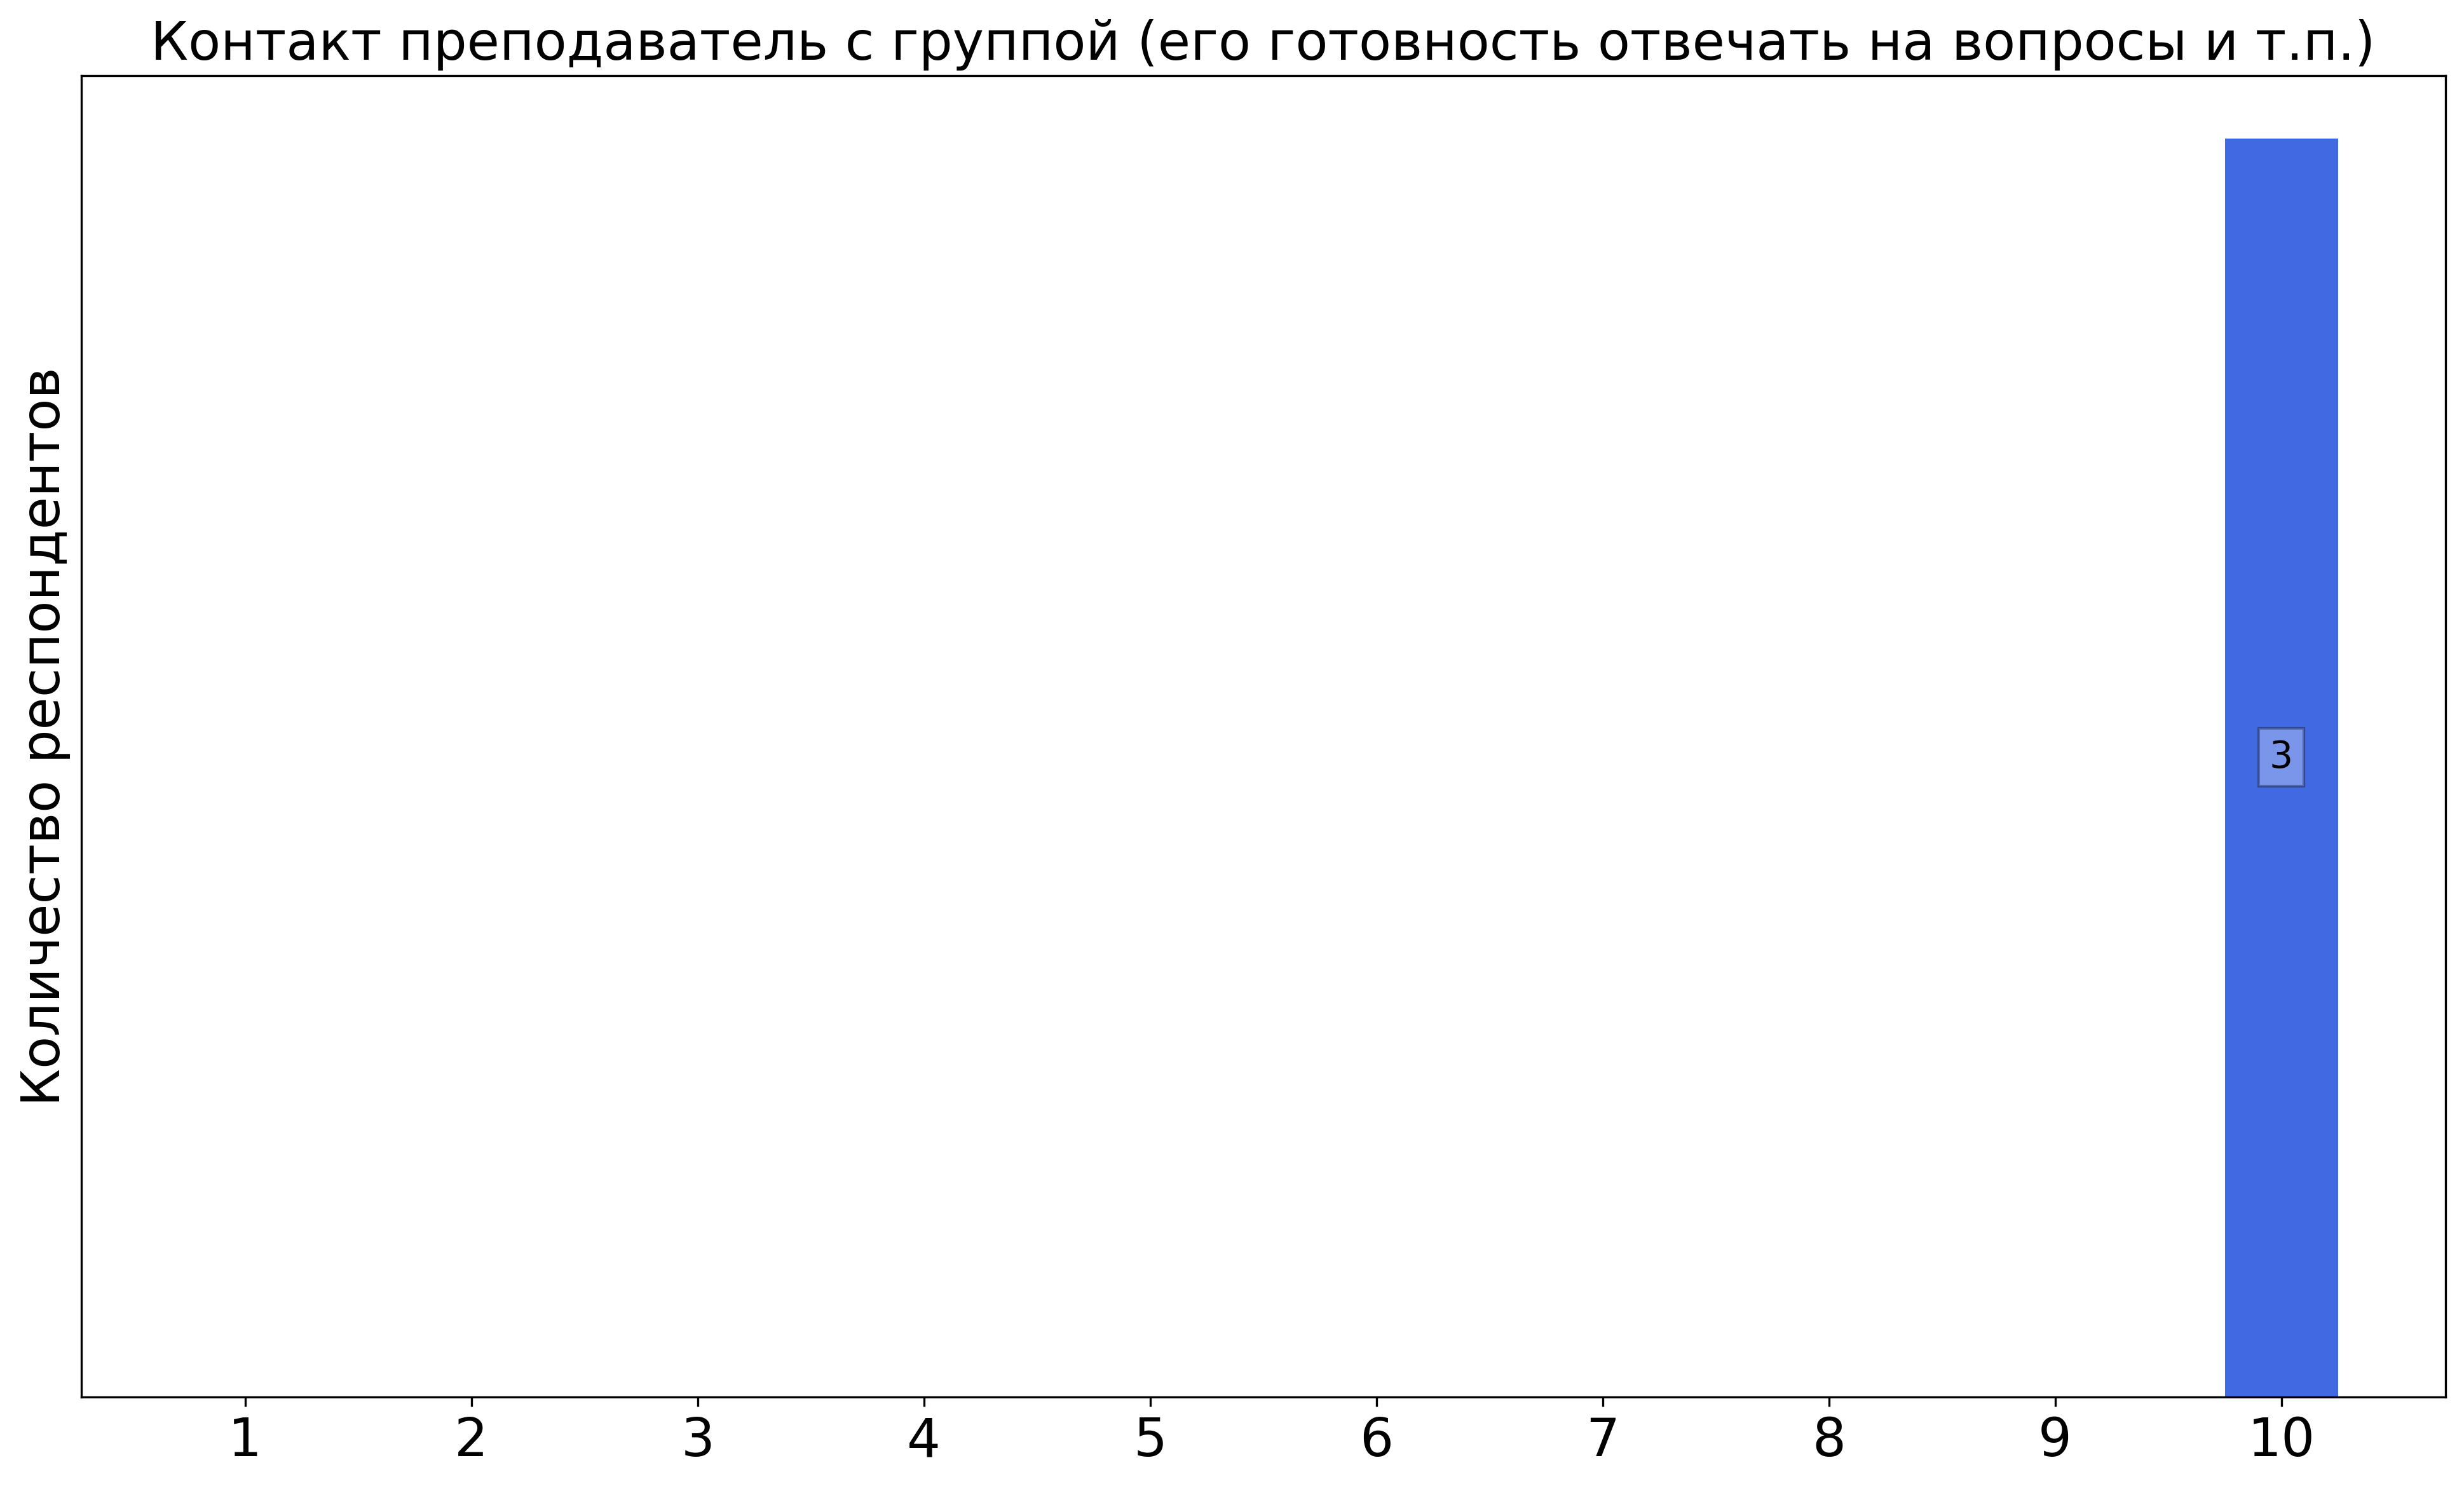
\includegraphics[width=\textwidth]{images/3 course/Аналоговая электроника/labniks-marks-Григорьев И.А.-0.png}
			\end{subfigure}
			\begin{subfigure}[b]{0.45\textwidth}
				\centering
				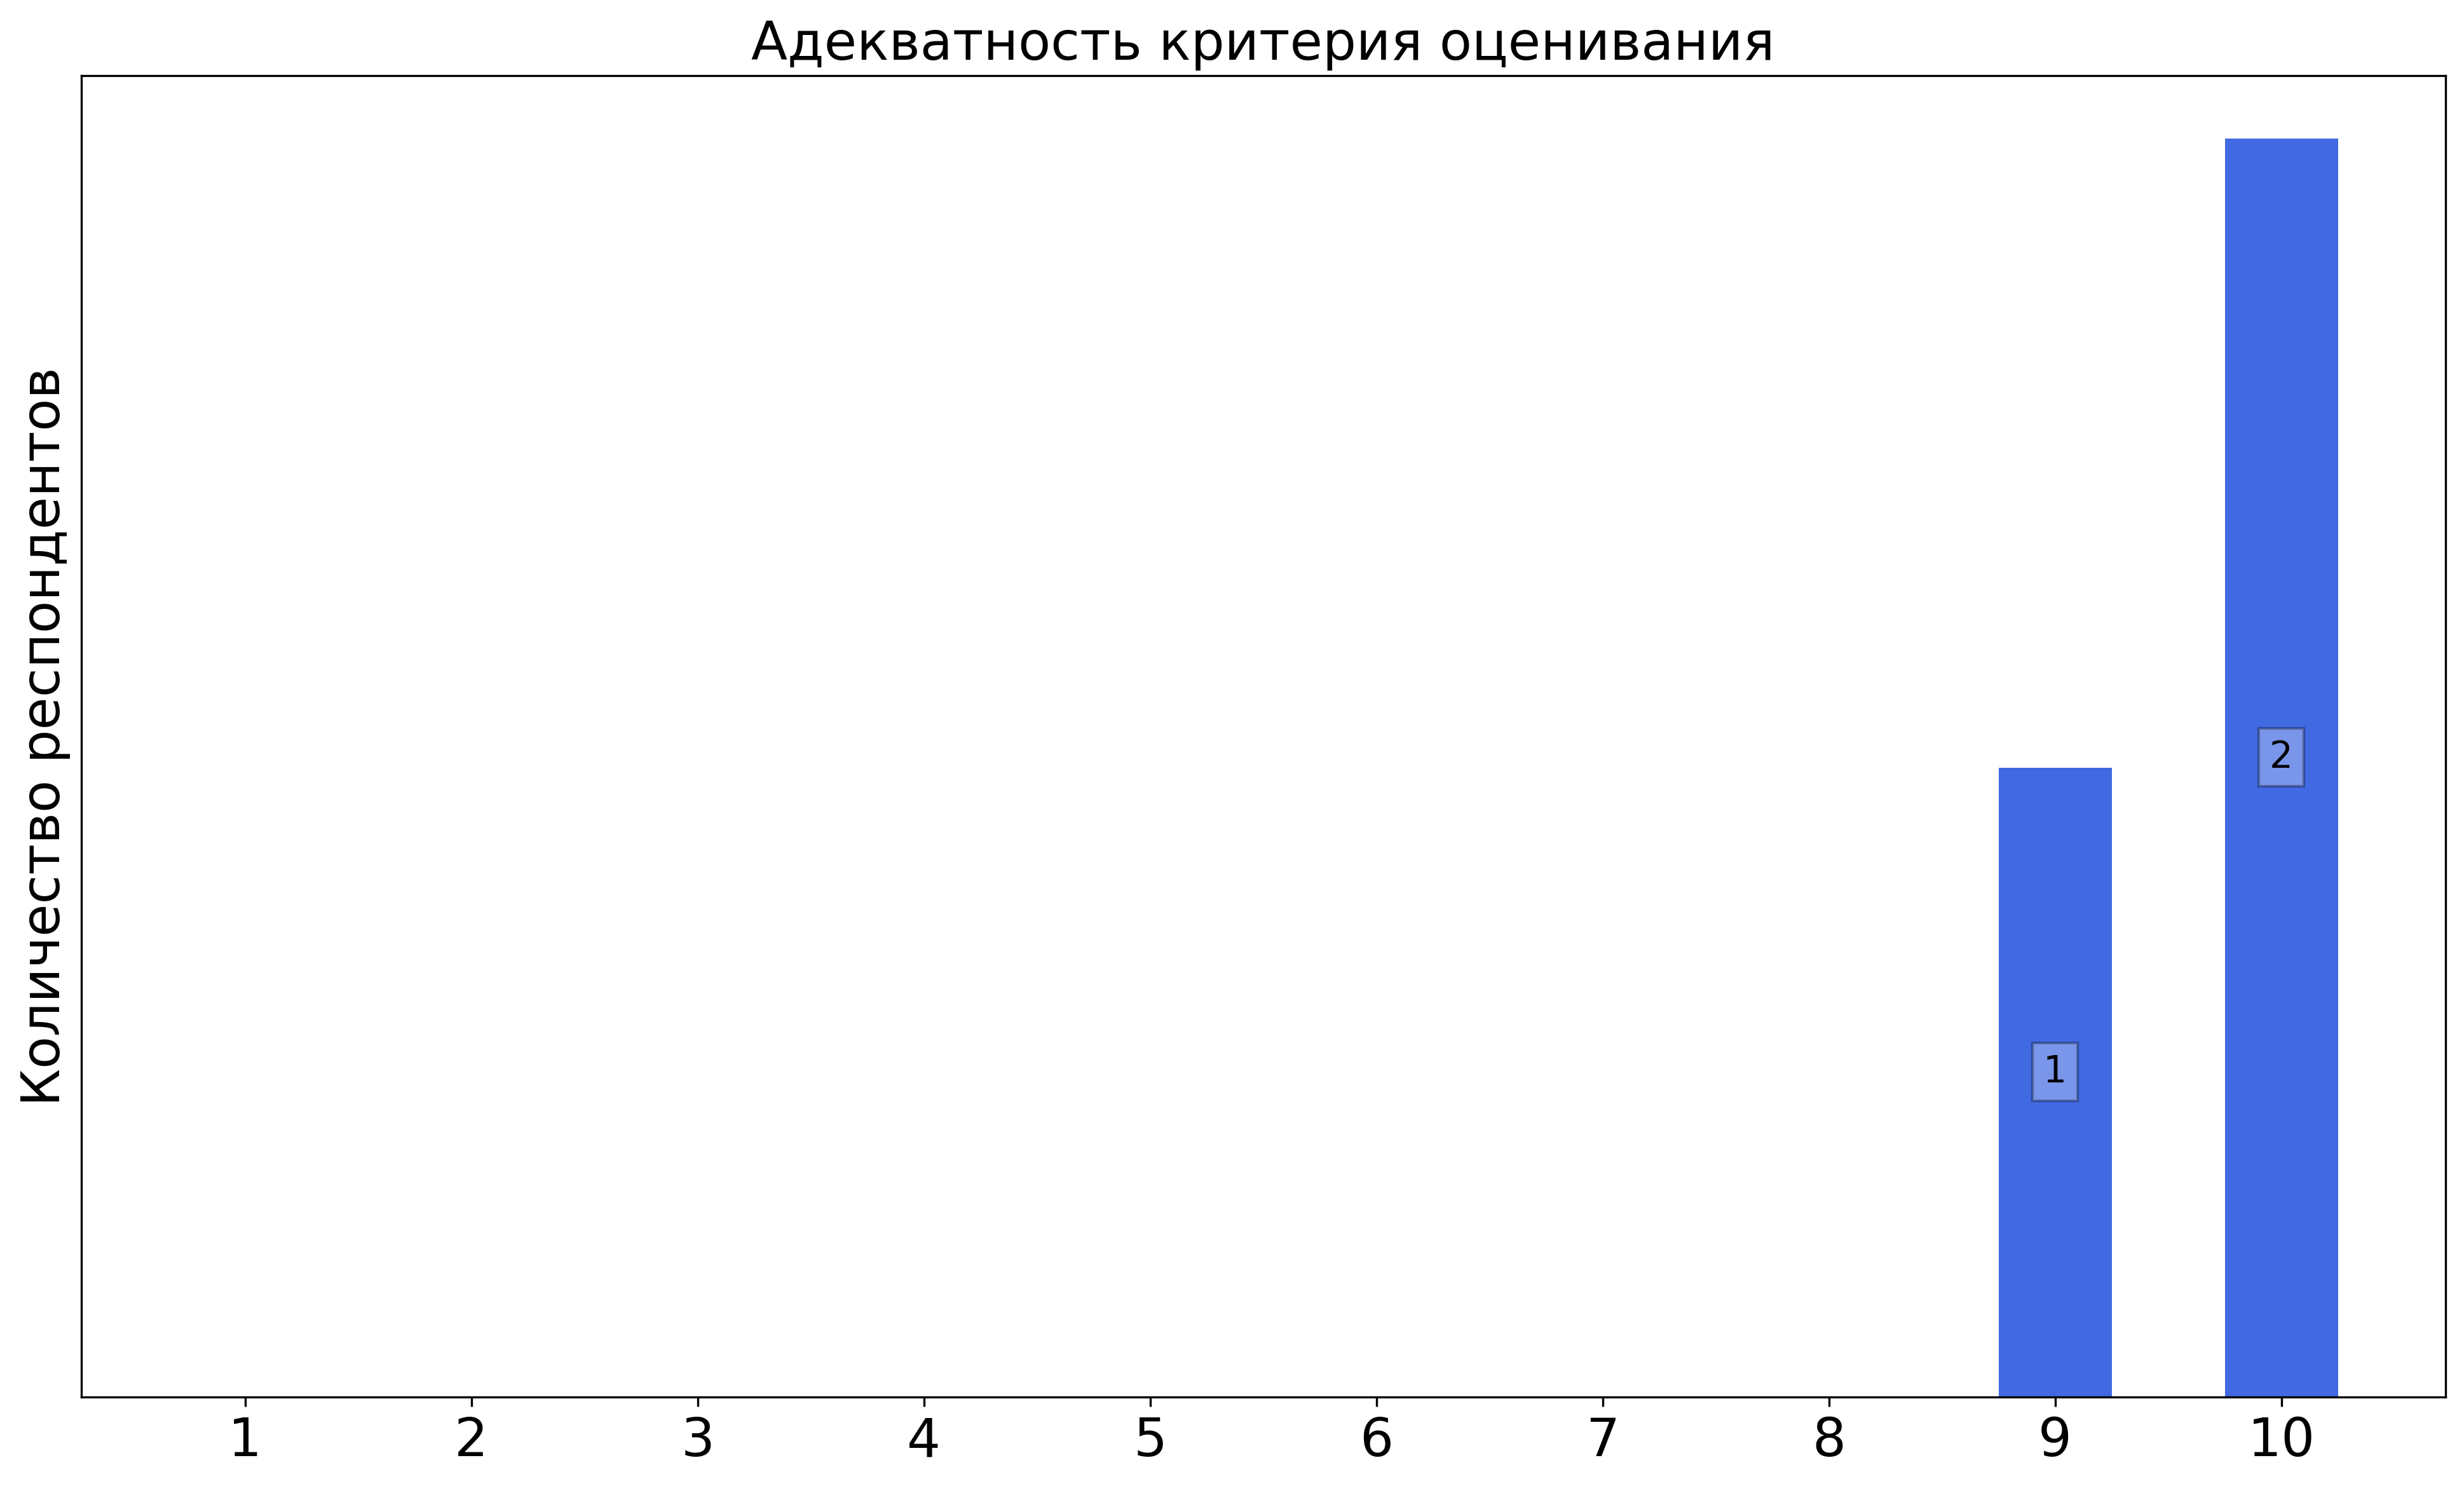
\includegraphics[width=\textwidth]{images/3 course/Аналоговая электроника/labniks-marks-Григорьев И.А.-1.png}
			\end{subfigure}
			\begin{subfigure}[b]{0.45\textwidth}
				\centering
				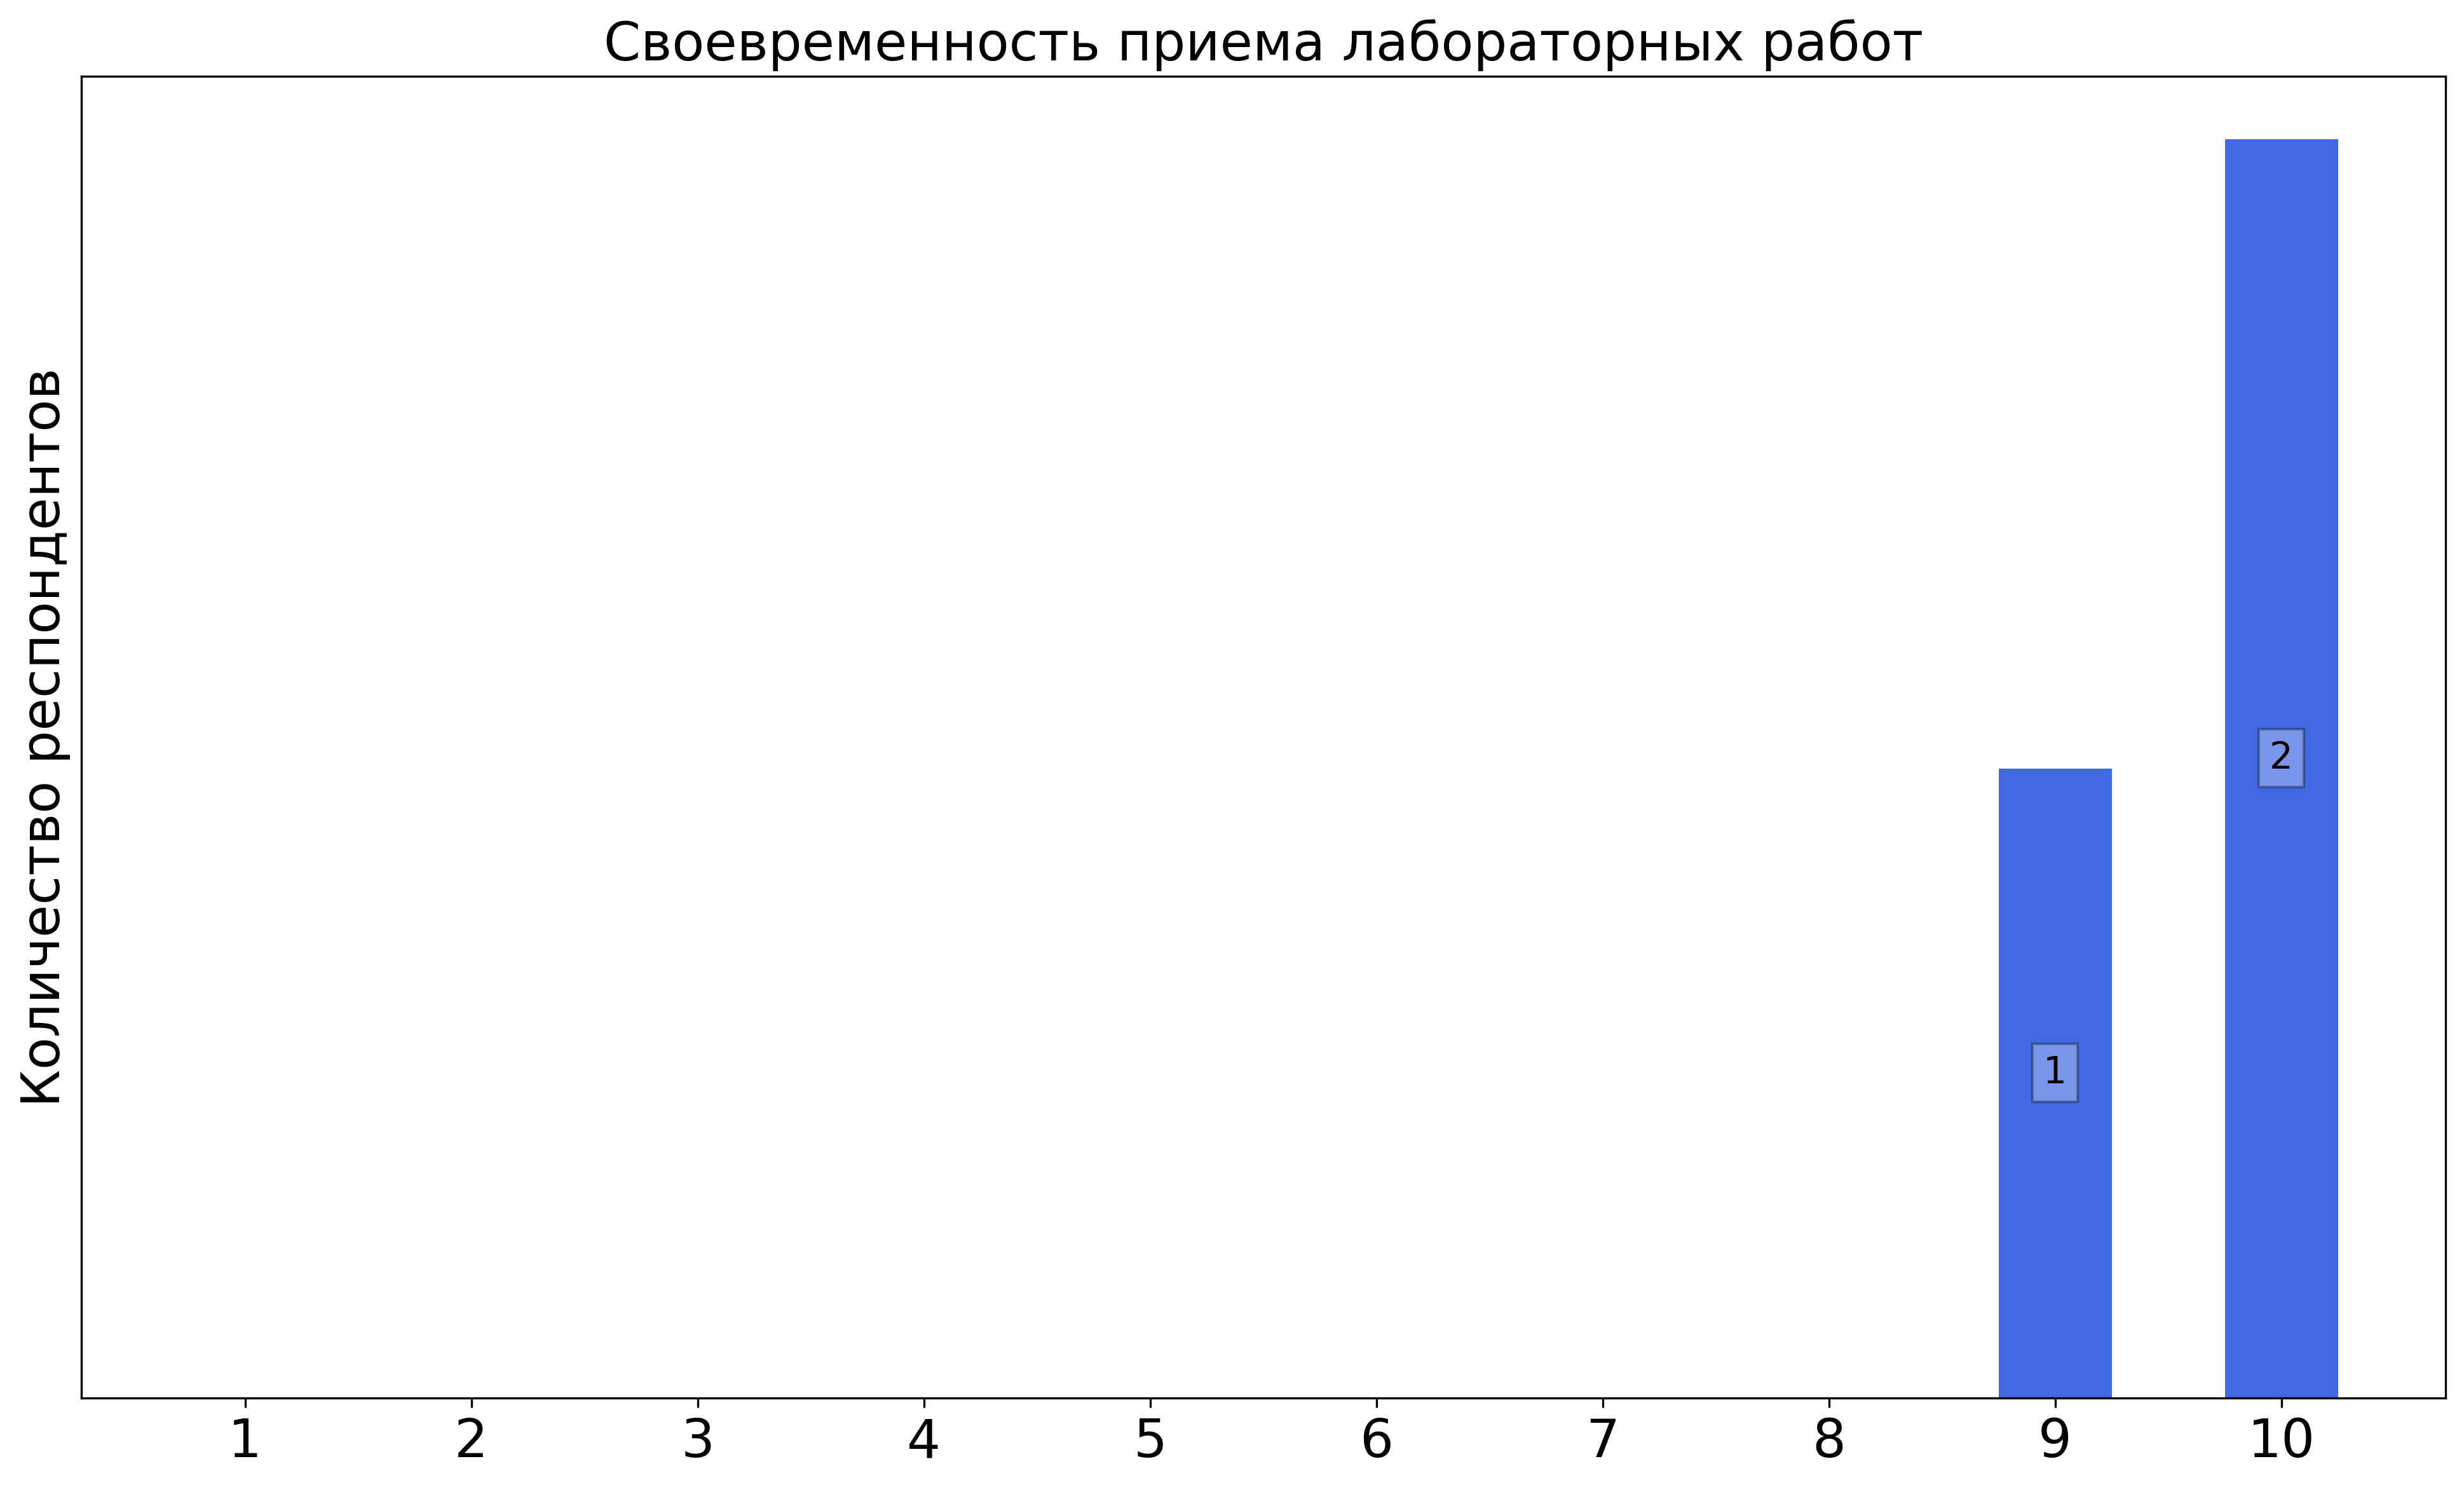
\includegraphics[width=\textwidth]{images/3 course/Аналоговая электроника/labniks-marks-Григорьев И.А.-2.png}
			\end{subfigure}
			\begin{subfigure}[b]{0.45\textwidth}
				\centering
				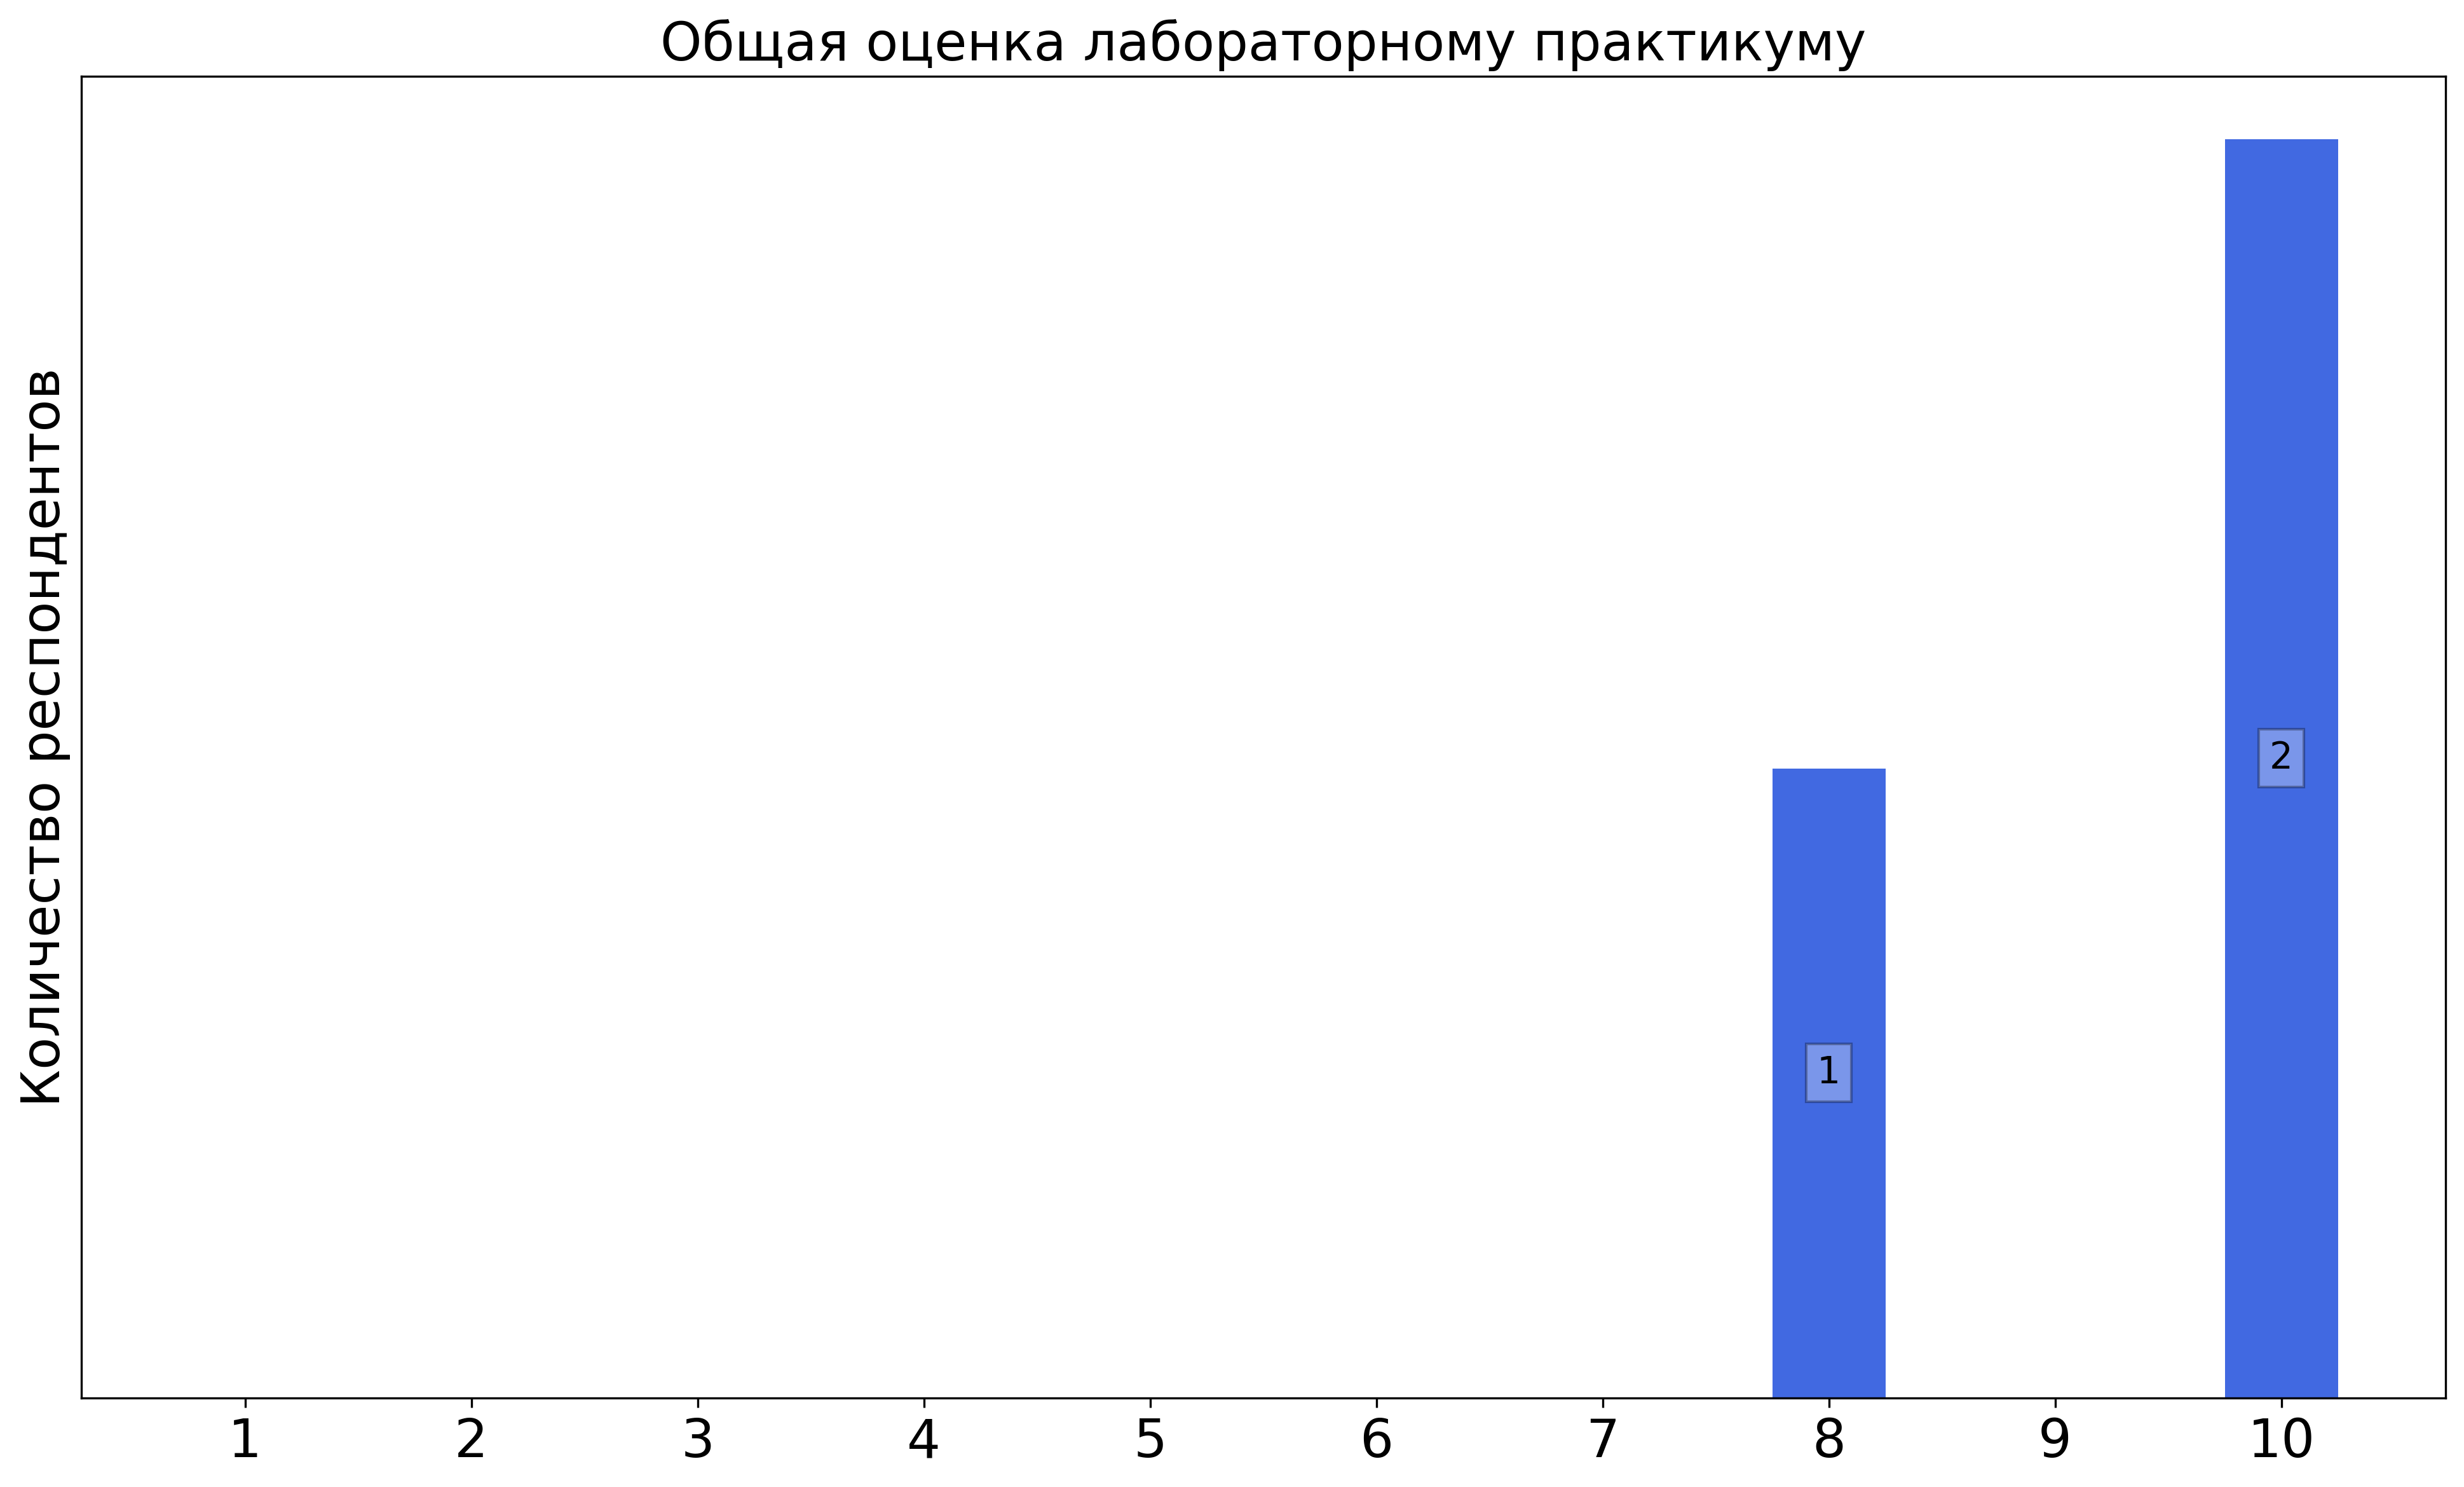
\includegraphics[width=\textwidth]{images/3 course/Аналоговая электроника/labniks-marks-Григорьев И.А.-3.png}
			\end{subfigure}	
			\caption{Оценки респондентов о качестве преподавания лабораторных работ}
		\end{figure}

		\textbf{Комментарии студентов о преподавателе\protect\footnote{сохранены оригинальные орфография и пунктуация}}
            \begin{commentbox} 
                хороший человек 
            \end{commentbox} 
        
            \begin{commentbox} 
                Сами лабы не очень интересные, опять что-то куда-то тыкаешь, но препод огонь. Материал свой знает и пытается донести, на сдачах требует понимания. Во время выполнения следит за ходом работы и помогает, у кого не совсем получается. Да и человек Григорьев хороший. 
            \end{commentbox}


    \subsubsection{Отзыв студентов о лабораторных работах. Преподаватель: Гутор А.В.}
		\begin{figure}[H]
			\centering
			\begin{subfigure}[b]{0.45\textwidth}
				\centering
				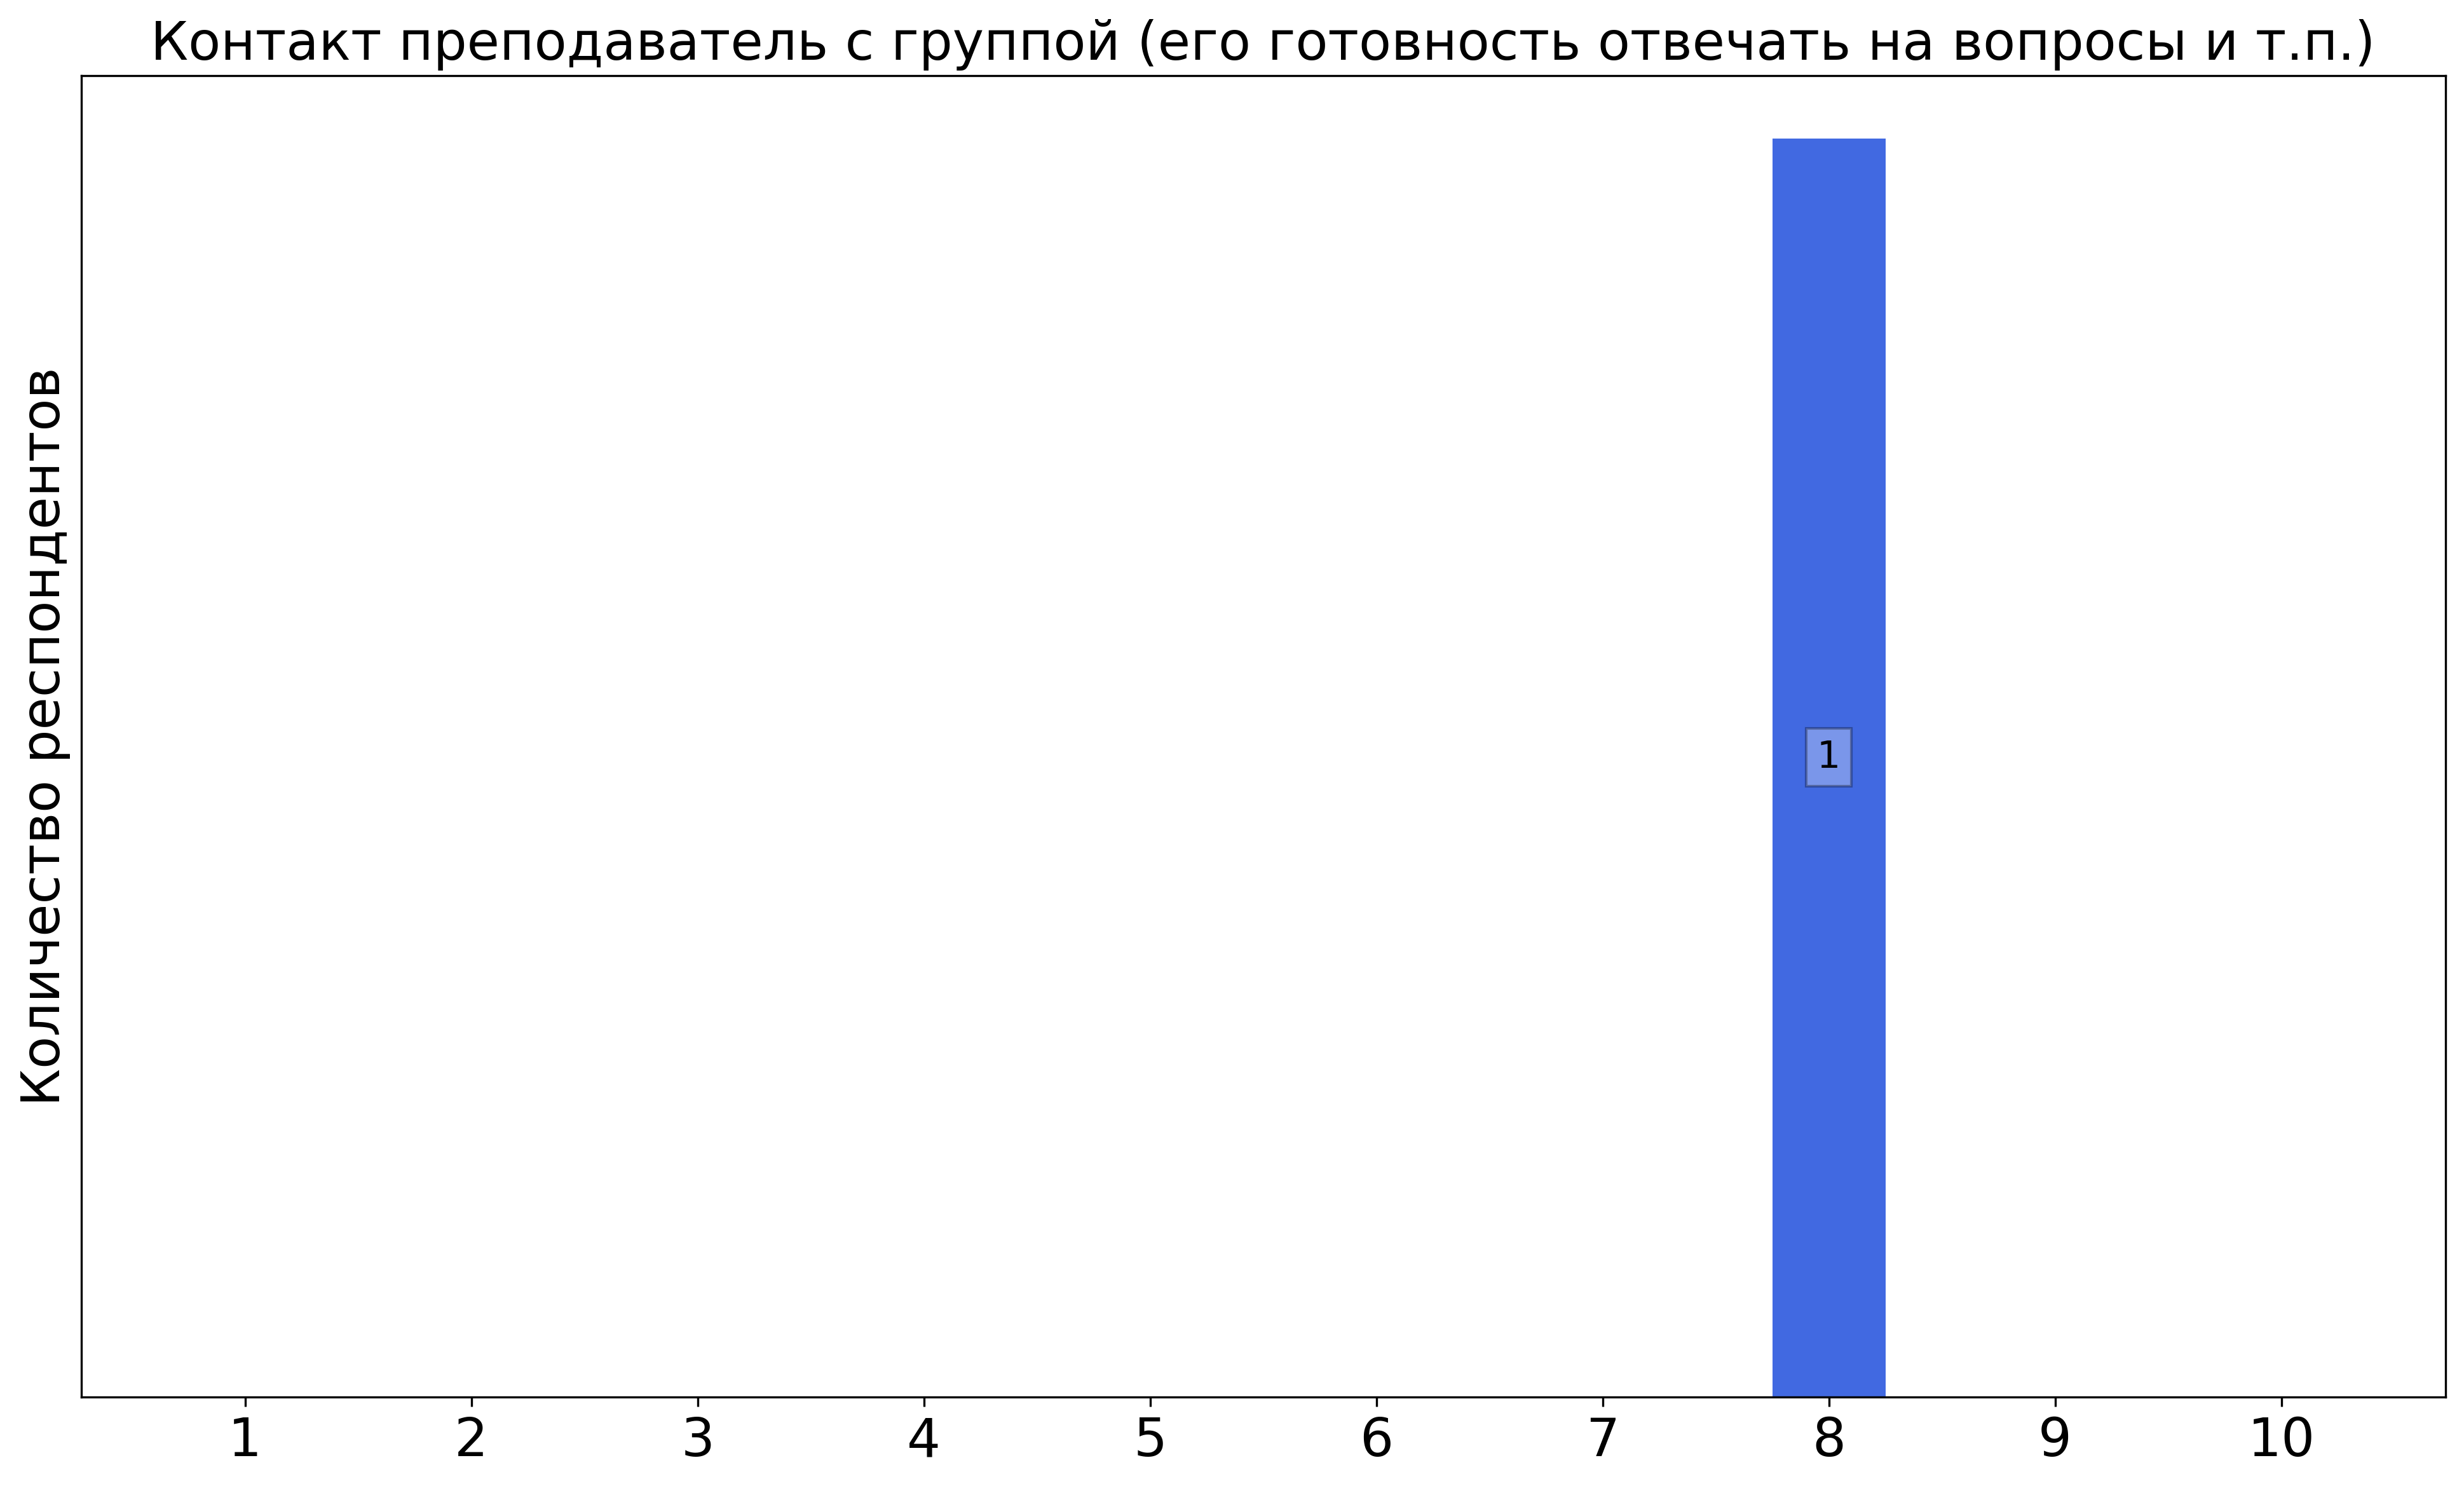
\includegraphics[width=\textwidth]{images/3 course/Аналоговая электроника/labniks-marks-Гутор А.В.-0.png}
			\end{subfigure}
			\begin{subfigure}[b]{0.45\textwidth}
				\centering
				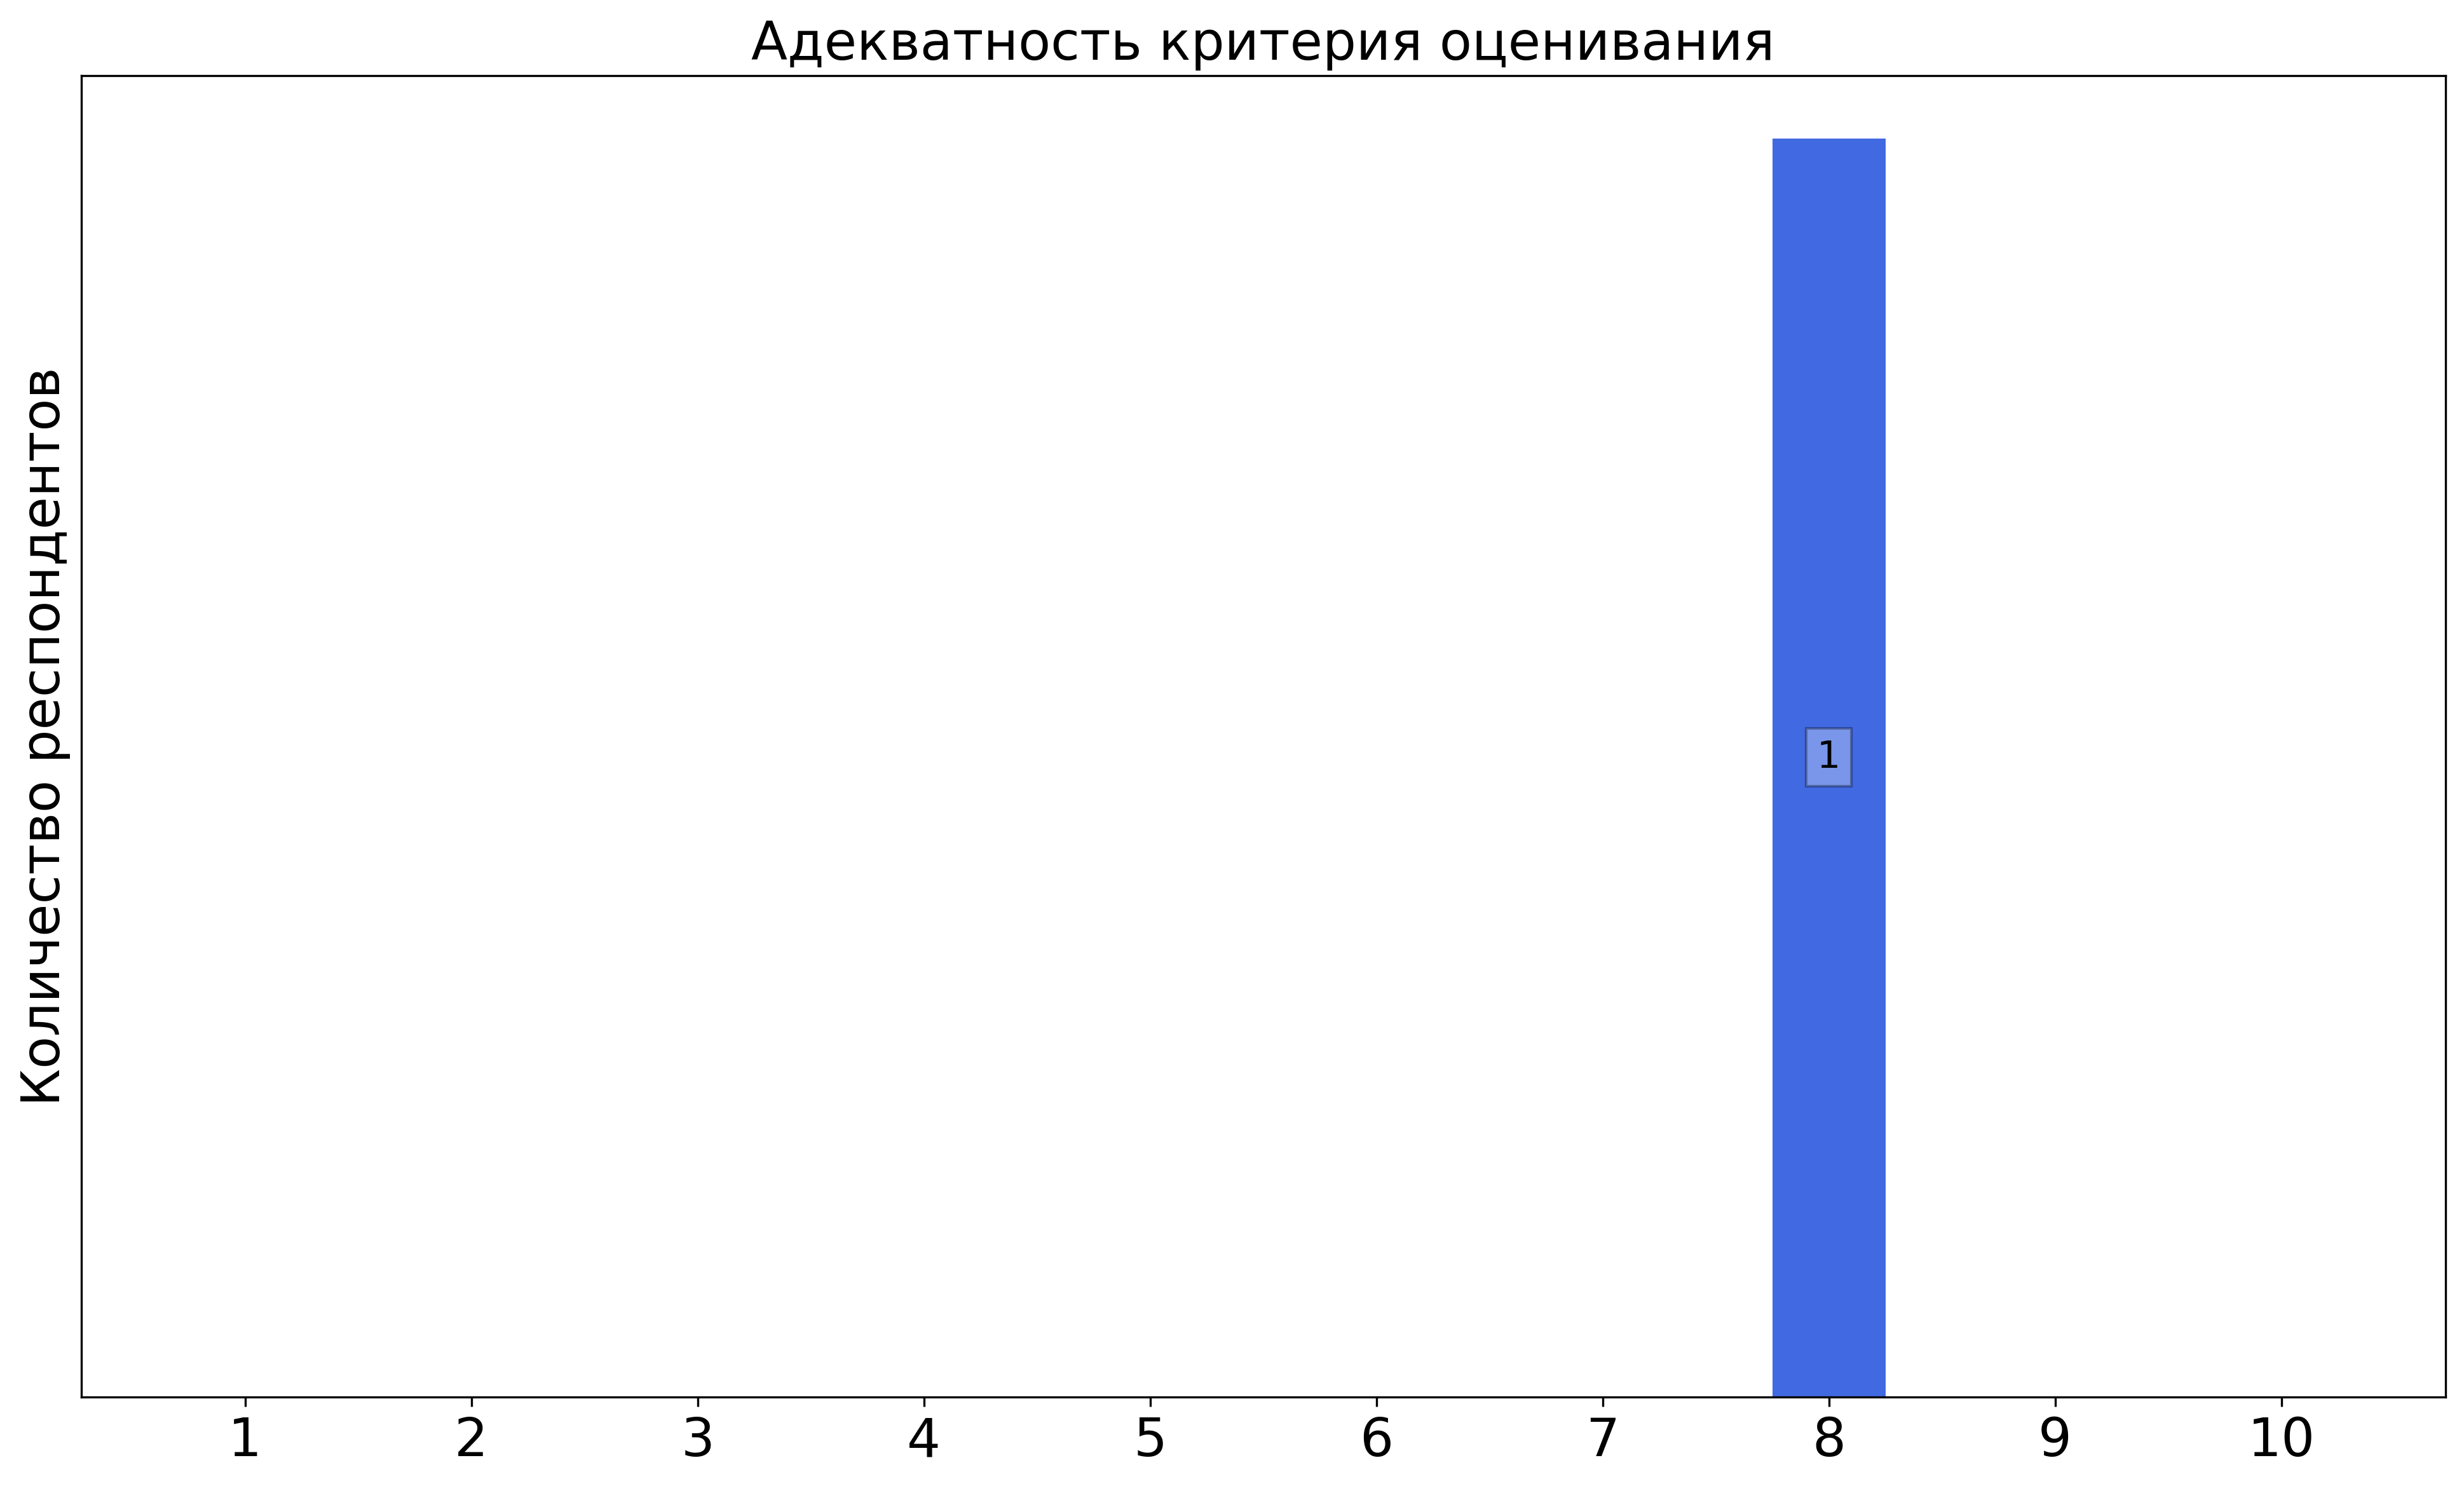
\includegraphics[width=\textwidth]{images/3 course/Аналоговая электроника/labniks-marks-Гутор А.В.-1.png}
			\end{subfigure}
			\begin{subfigure}[b]{0.45\textwidth}
				\centering
				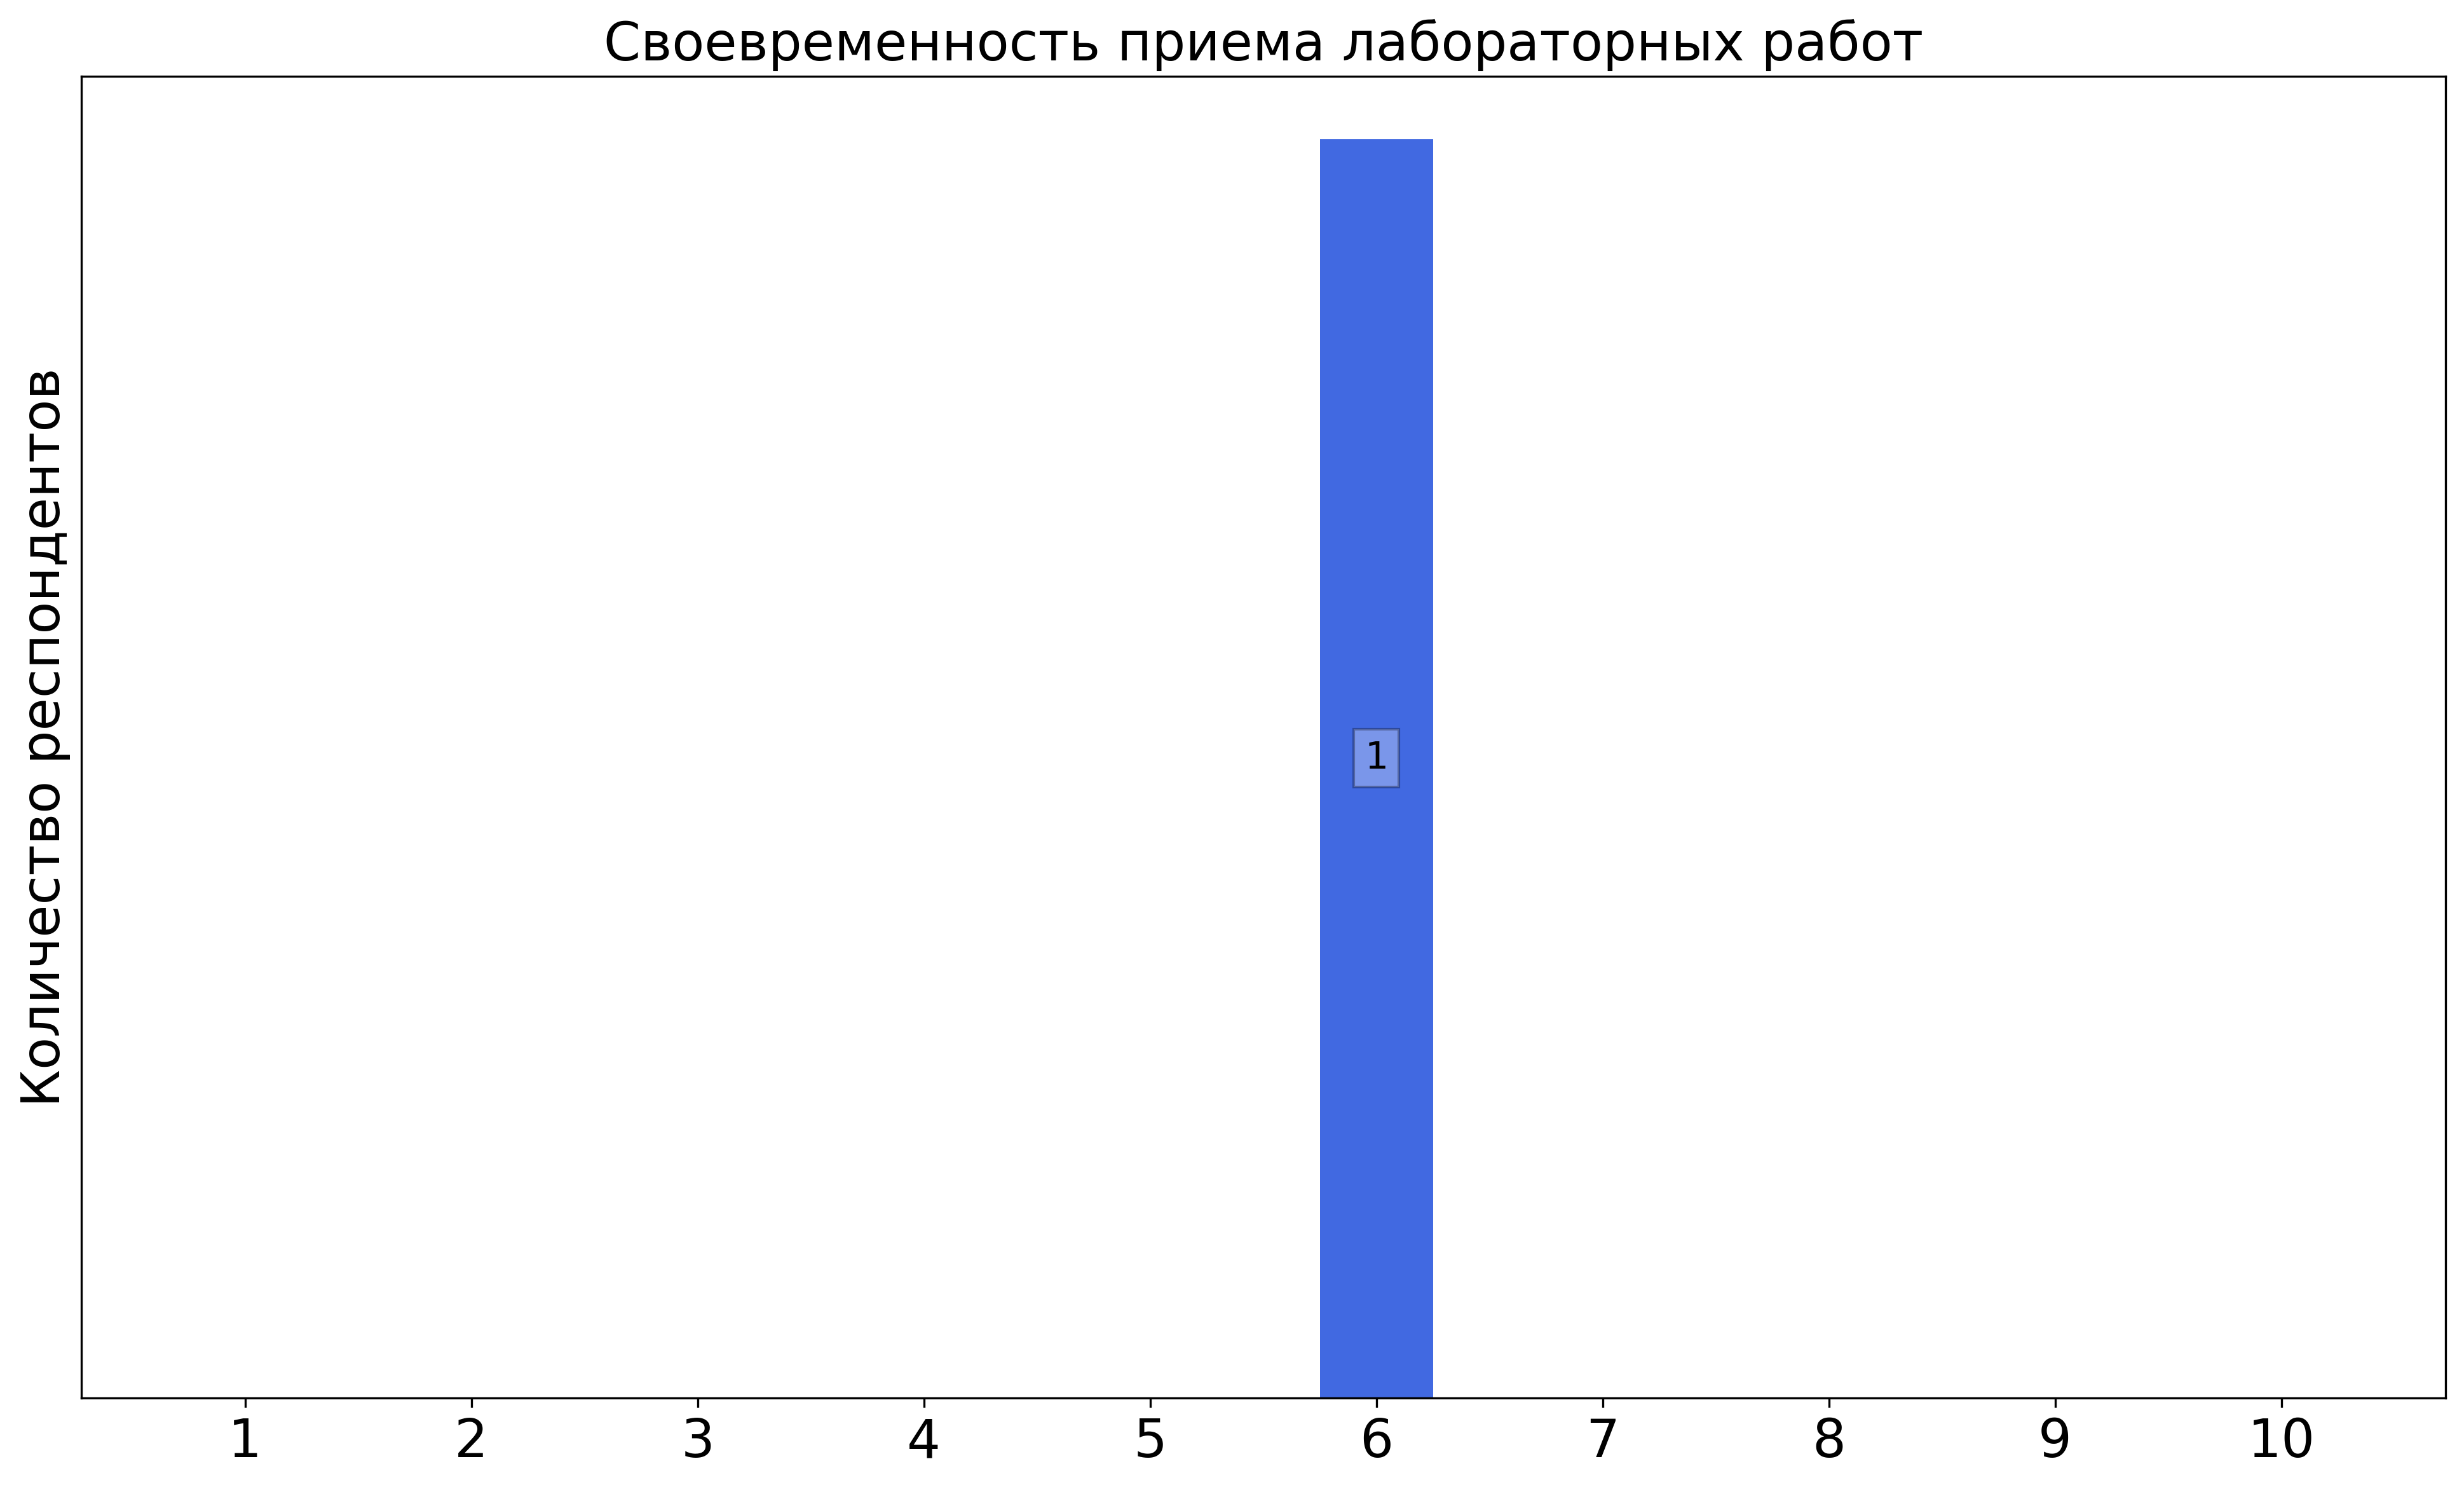
\includegraphics[width=\textwidth]{images/3 course/Аналоговая электроника/labniks-marks-Гутор А.В.-2.png}
			\end{subfigure}
			\begin{subfigure}[b]{0.45\textwidth}
				\centering
				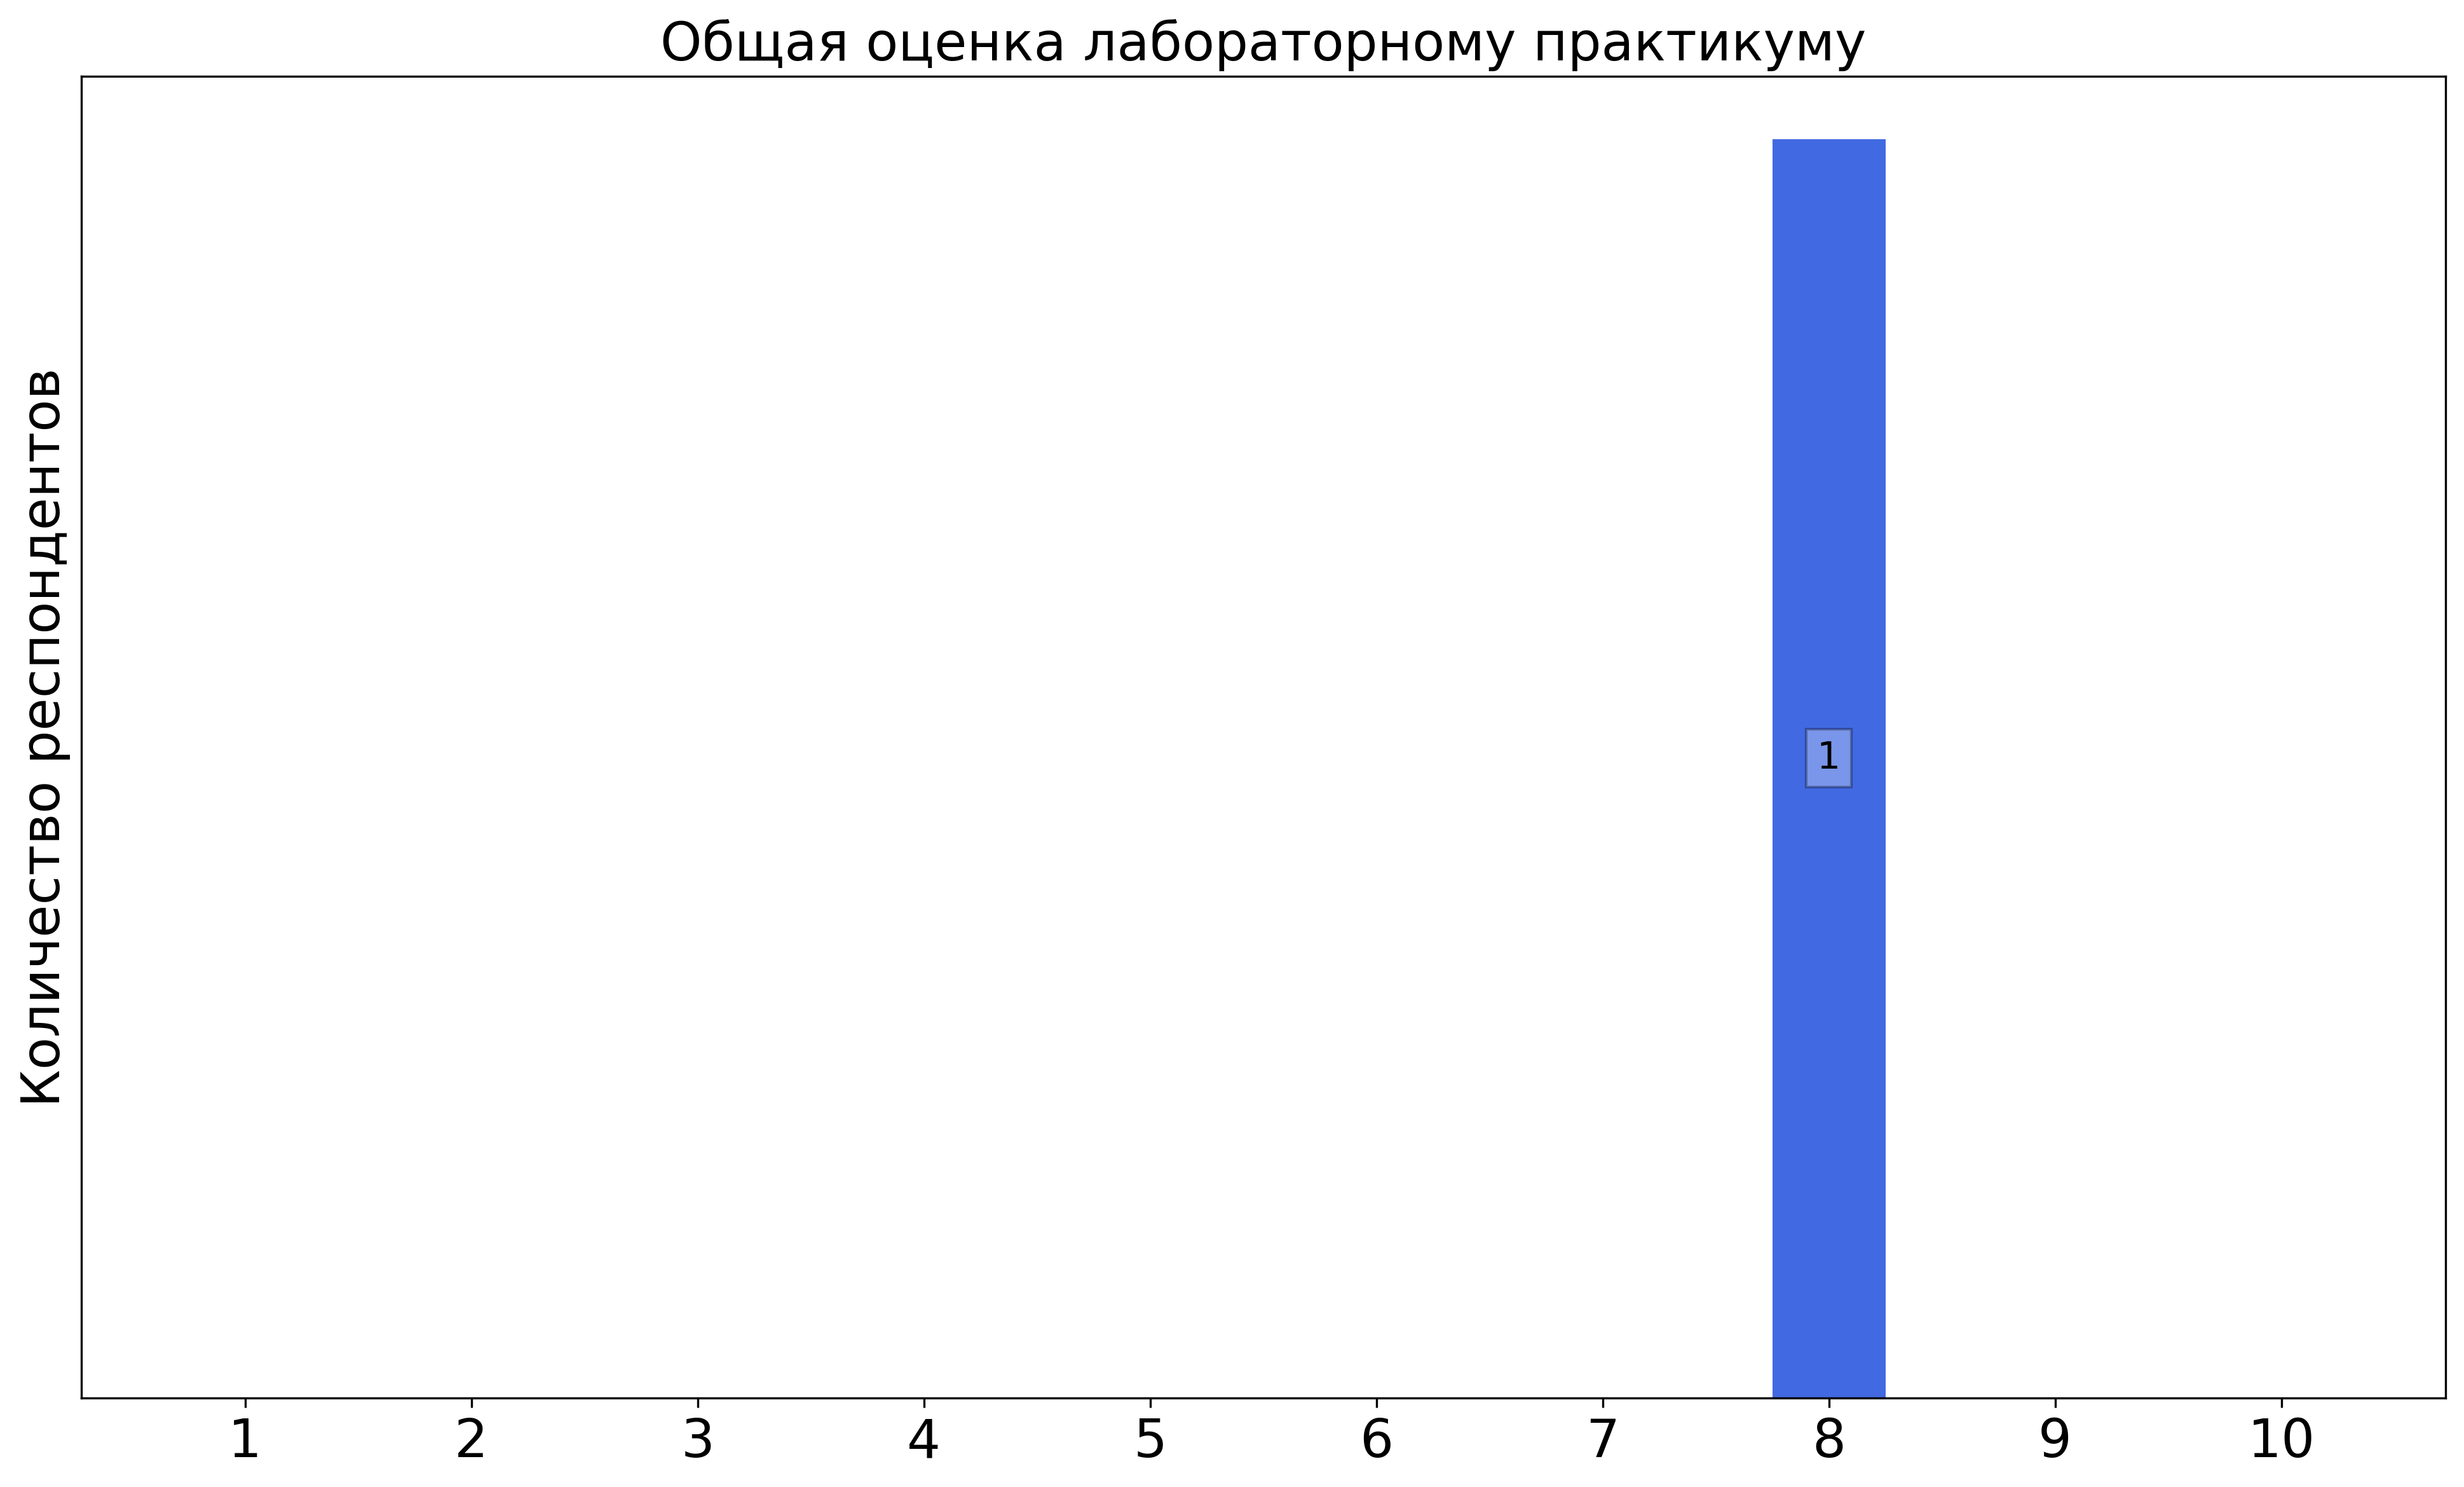
\includegraphics[width=\textwidth]{images/3 course/Аналоговая электроника/labniks-marks-Гутор А.В.-3.png}
			\end{subfigure}	
			\caption{Оценки респондентов о качестве преподавания лабораторных работ}
		\end{figure}

        
    \subsubsection{Отзыв студентов о лабораторных работах. Преподаватель: Дунаева М.А.}
		\begin{figure}[H]
			\centering
			\begin{subfigure}[b]{0.45\textwidth}
				\centering
				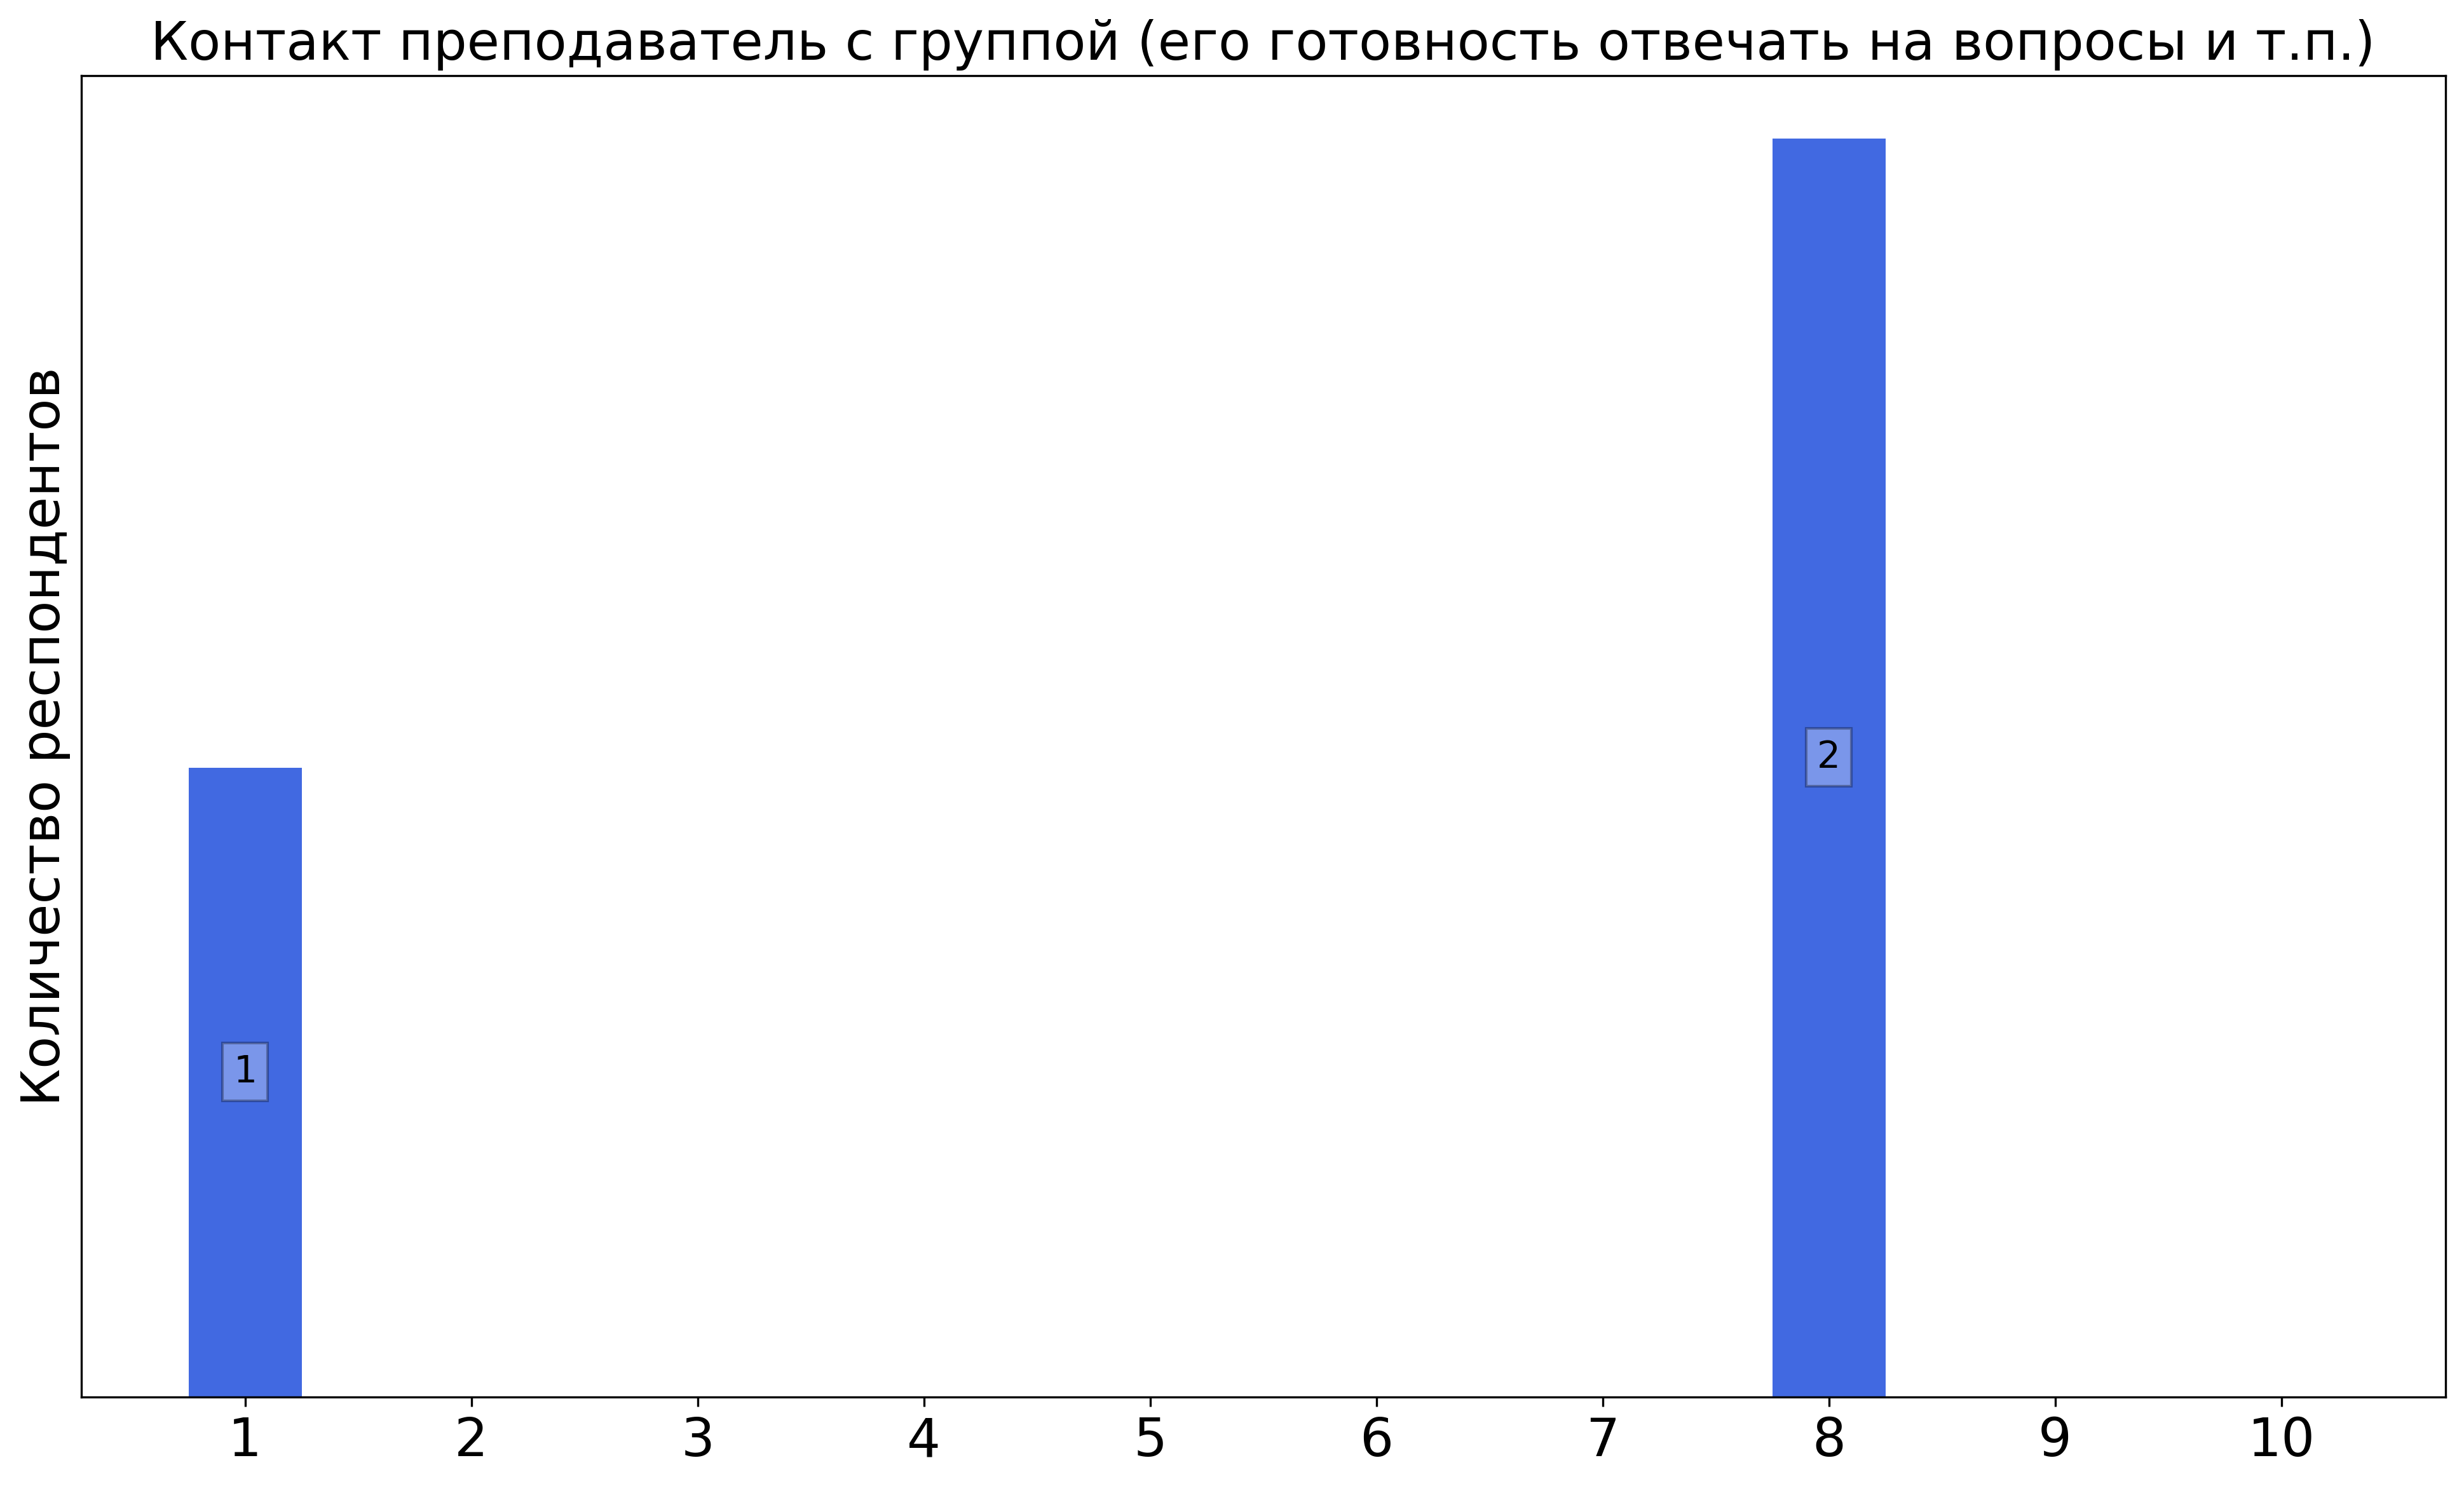
\includegraphics[width=\textwidth]{images/3 course/Аналоговая электроника/labniks-marks-Дунаева М.А.-0.png}
			\end{subfigure}
			\begin{subfigure}[b]{0.45\textwidth}
				\centering
				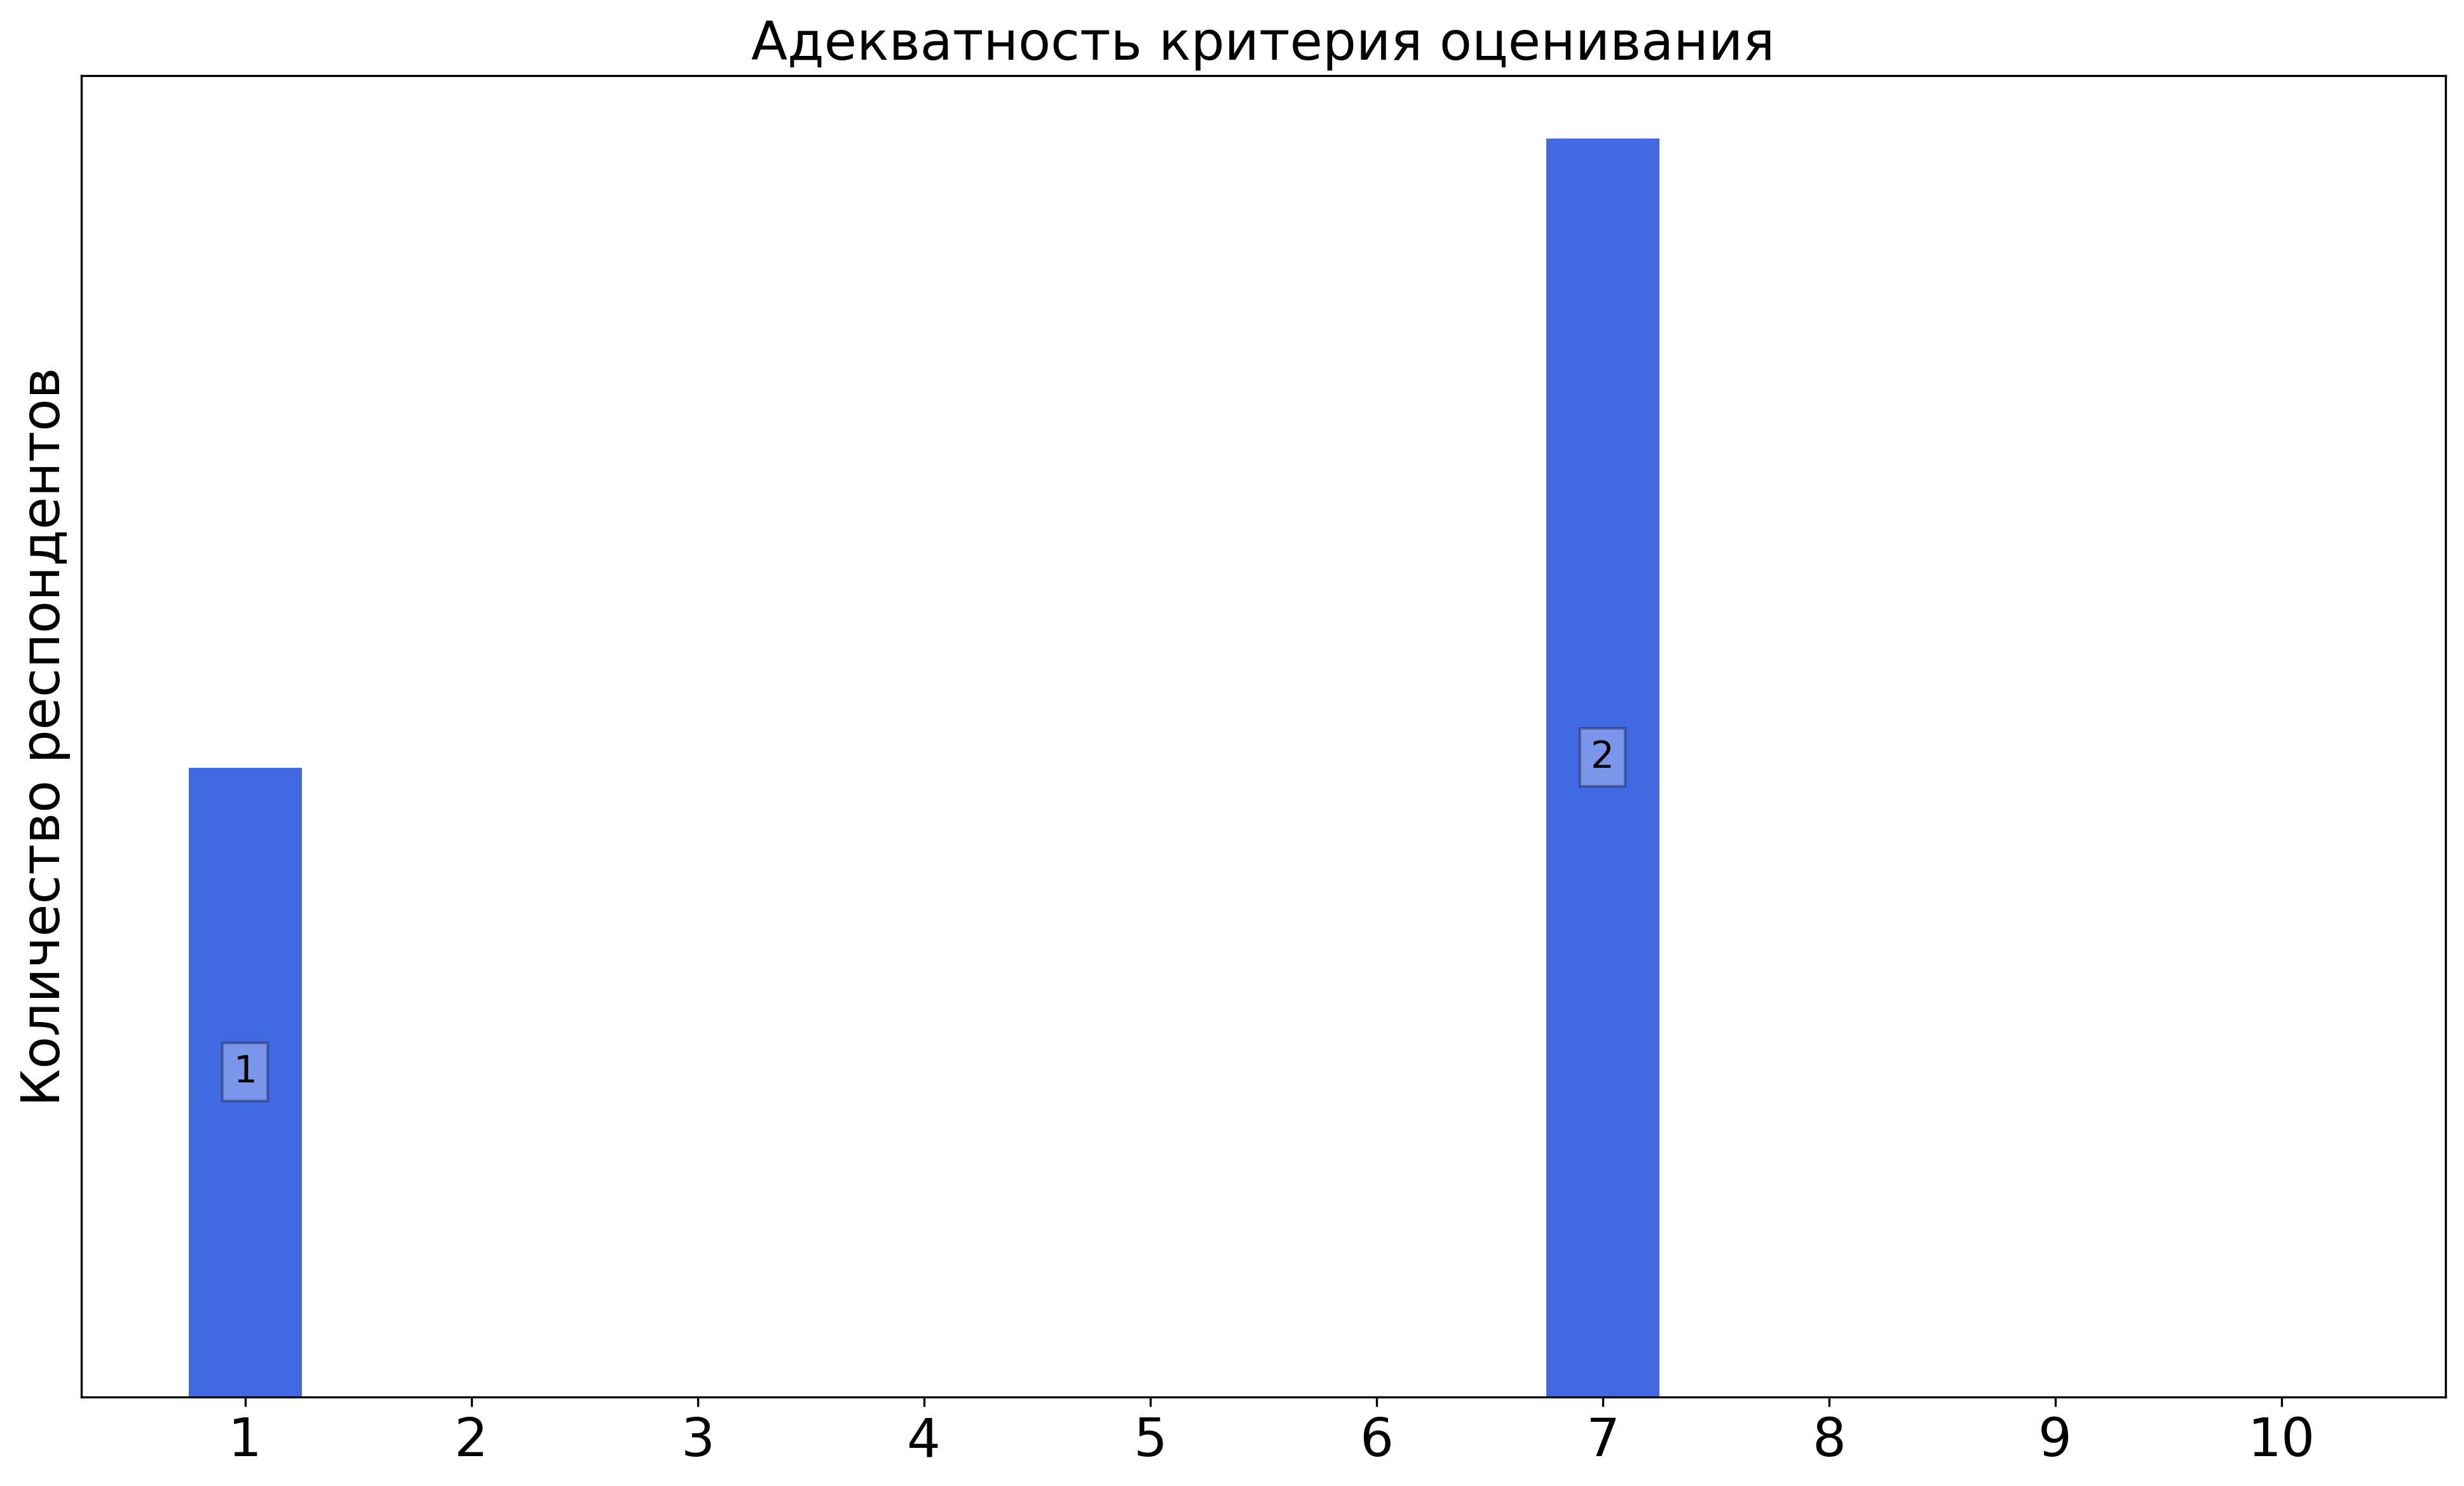
\includegraphics[width=\textwidth]{images/3 course/Аналоговая электроника/labniks-marks-Дунаева М.А.-1.png}
			\end{subfigure}
			\begin{subfigure}[b]{0.45\textwidth}
				\centering
				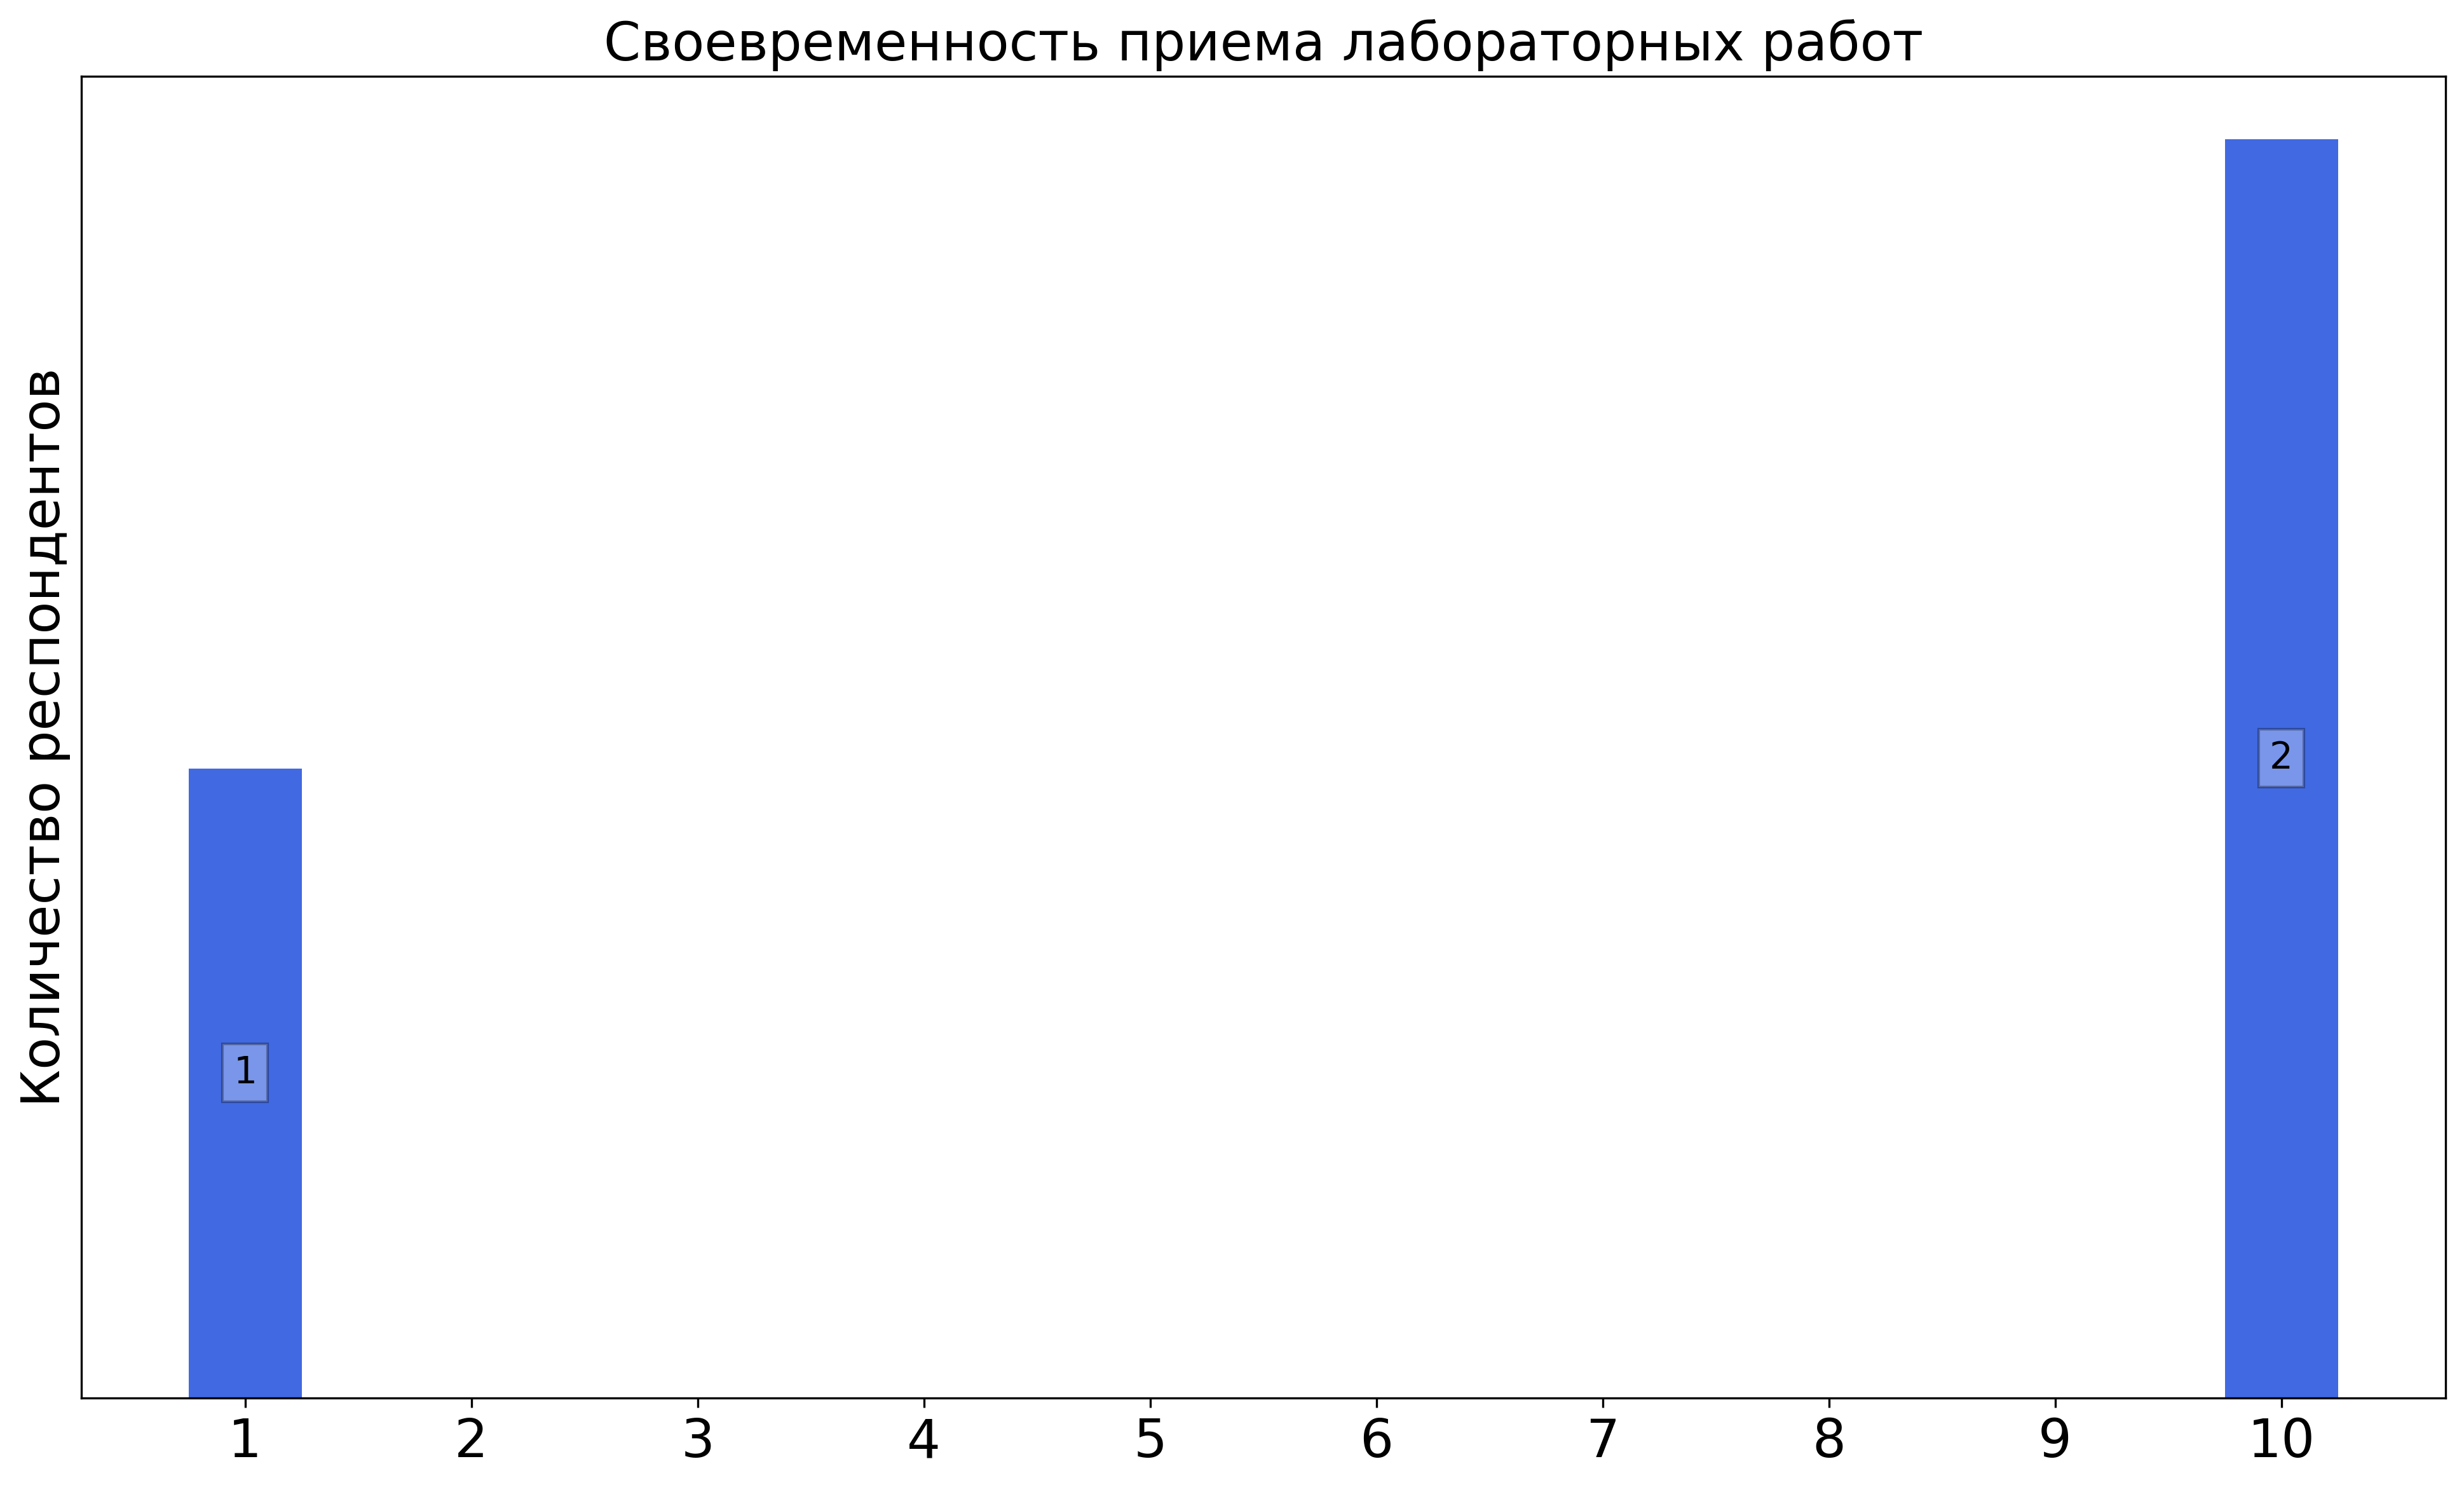
\includegraphics[width=\textwidth]{images/3 course/Аналоговая электроника/labniks-marks-Дунаева М.А.-2.png}
			\end{subfigure}
			\begin{subfigure}[b]{0.45\textwidth}
				\centering
				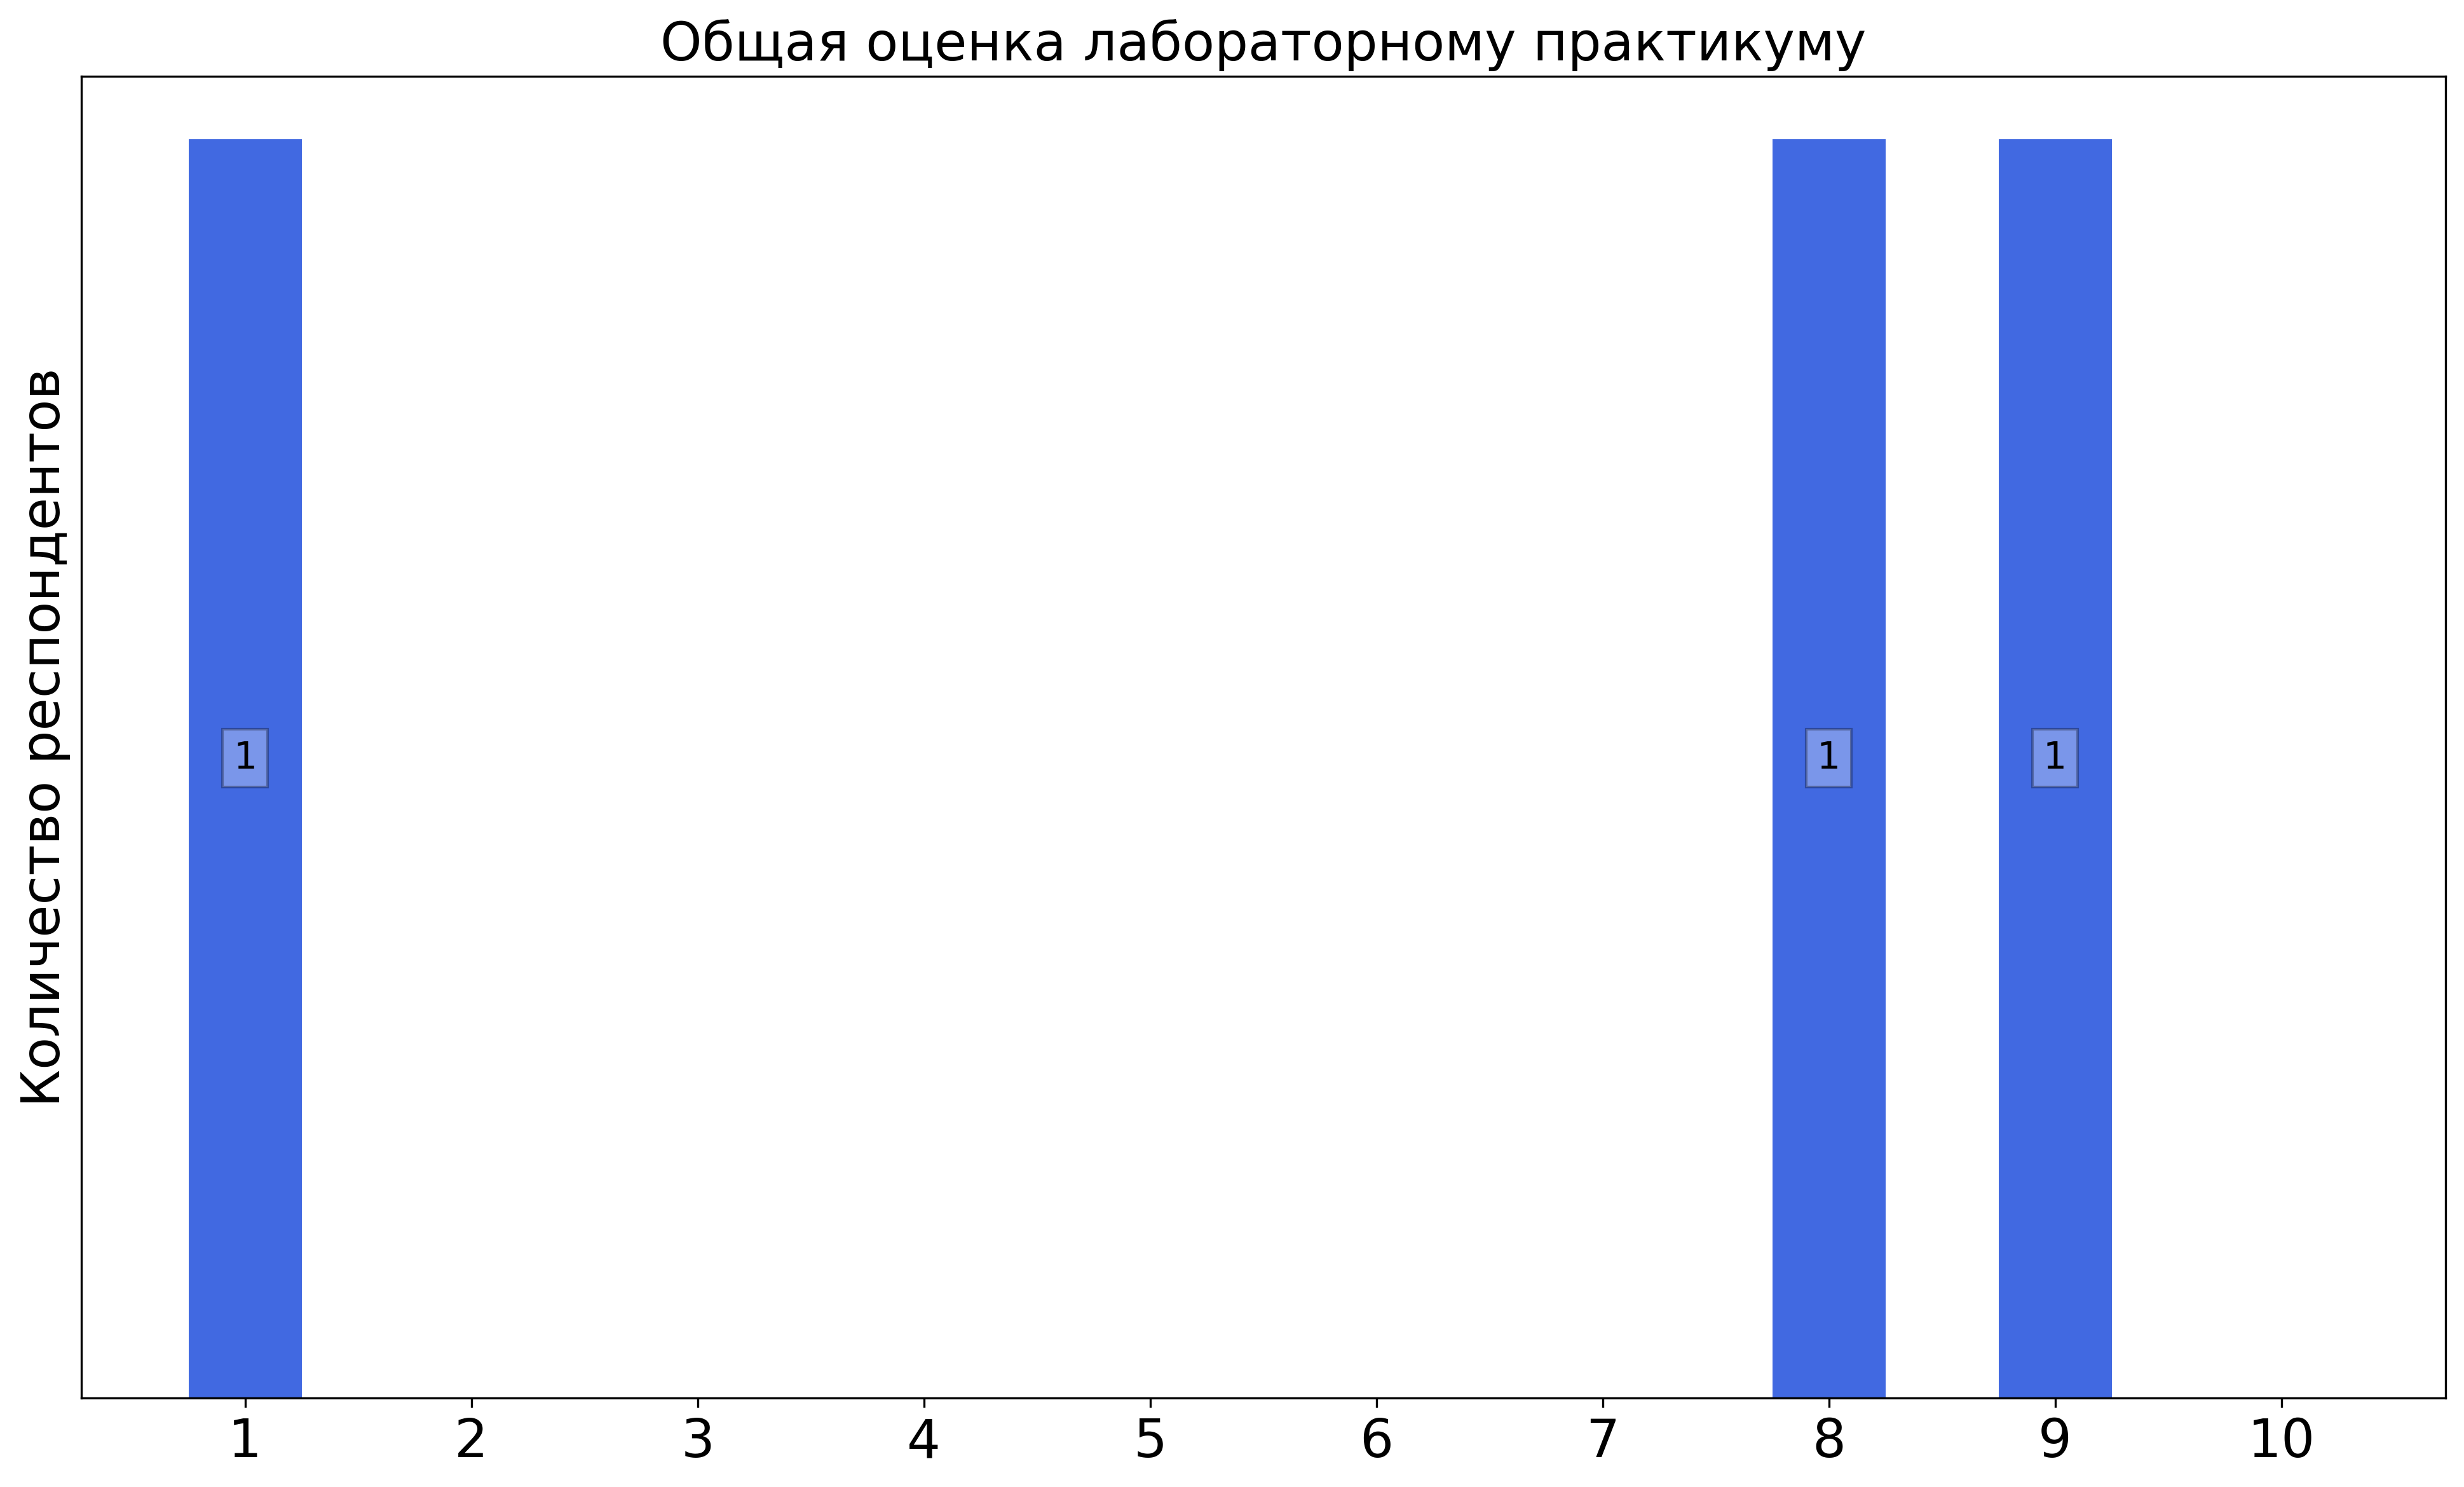
\includegraphics[width=\textwidth]{images/3 course/Аналоговая электроника/labniks-marks-Дунаева М.А.-3.png}
			\end{subfigure}	
			\caption{Оценки респондентов о качестве преподавания лабораторных работ}
		\end{figure}

		\textbf{Комментарии студентов о преподавателе\protect\footnote{сохранены оригинальные орфография и пунктуация}}
            \begin{commentbox} 
                На вопросы по лабам отвечает.  
            \end{commentbox} 
        

    \subsubsection{Отзыв студентов о лабораторных работах. Преподаватель: Зарипов Р.А.}
		\begin{figure}[H]
			\centering
			\begin{subfigure}[b]{0.45\textwidth}
				\centering
				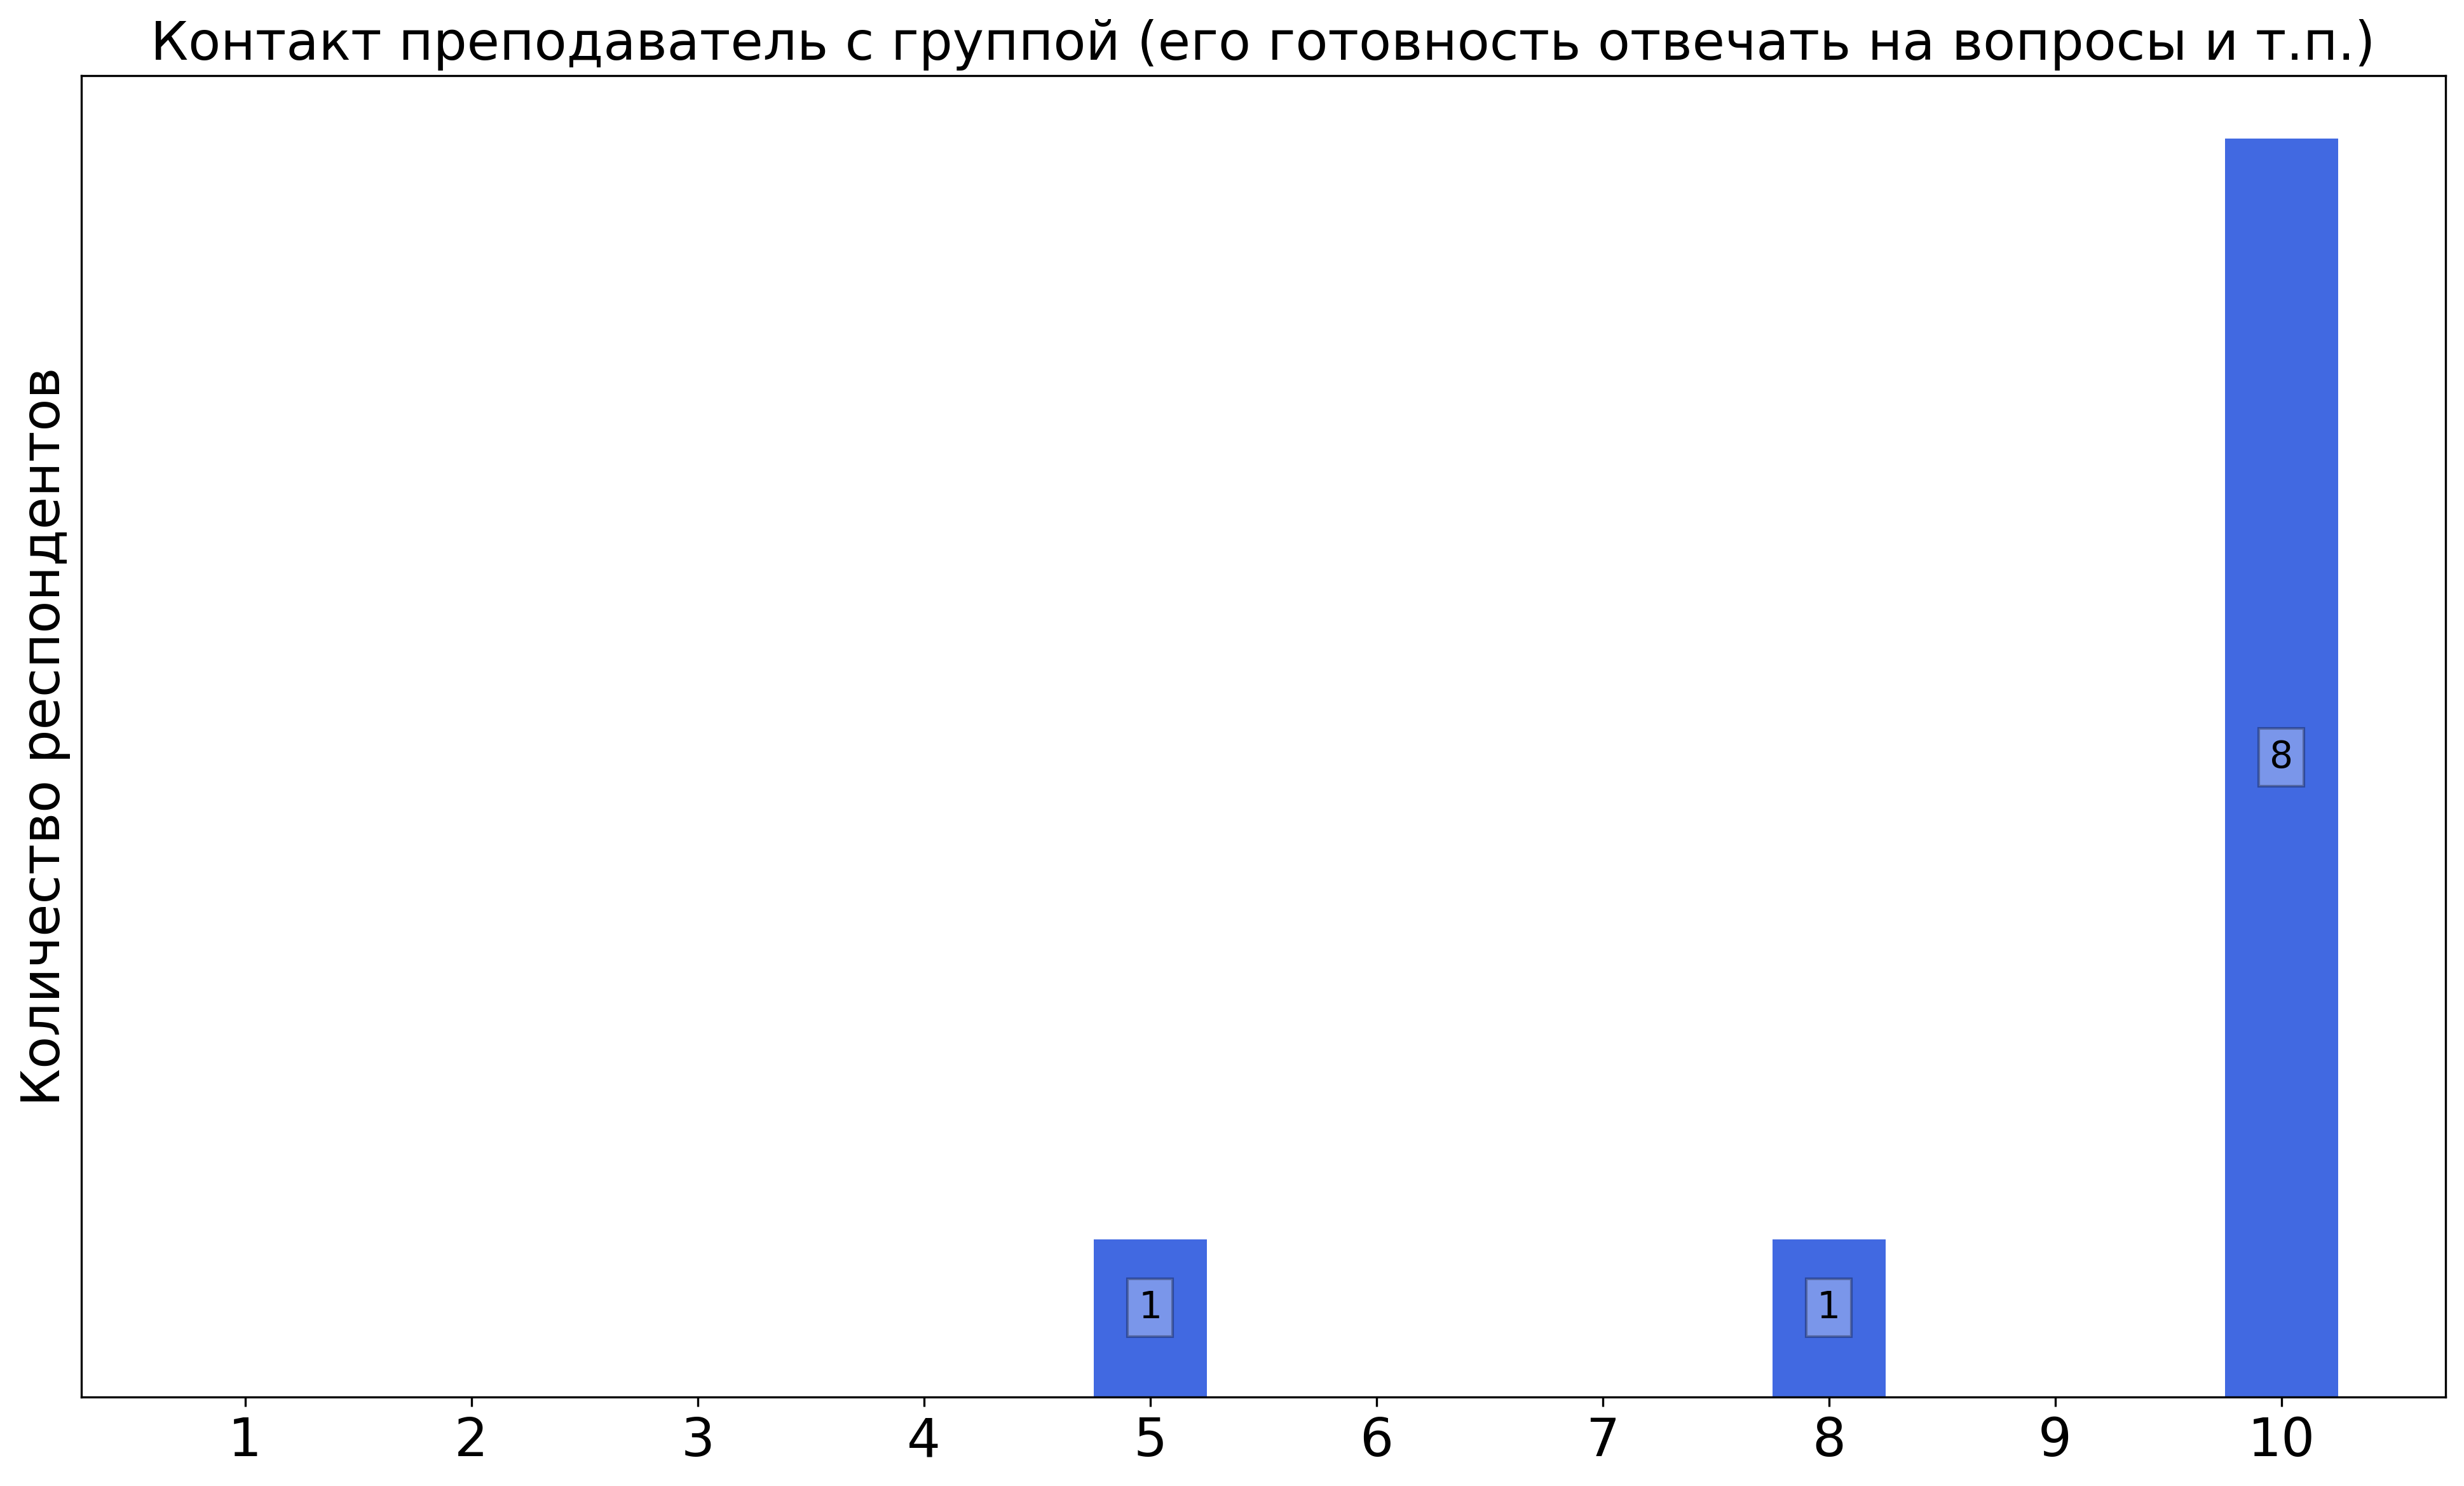
\includegraphics[width=\textwidth]{images/3 course/Аналоговая электроника/labniks-marks-Зарипов Р.А.-0.png}
			\end{subfigure}
			\begin{subfigure}[b]{0.45\textwidth}
				\centering
				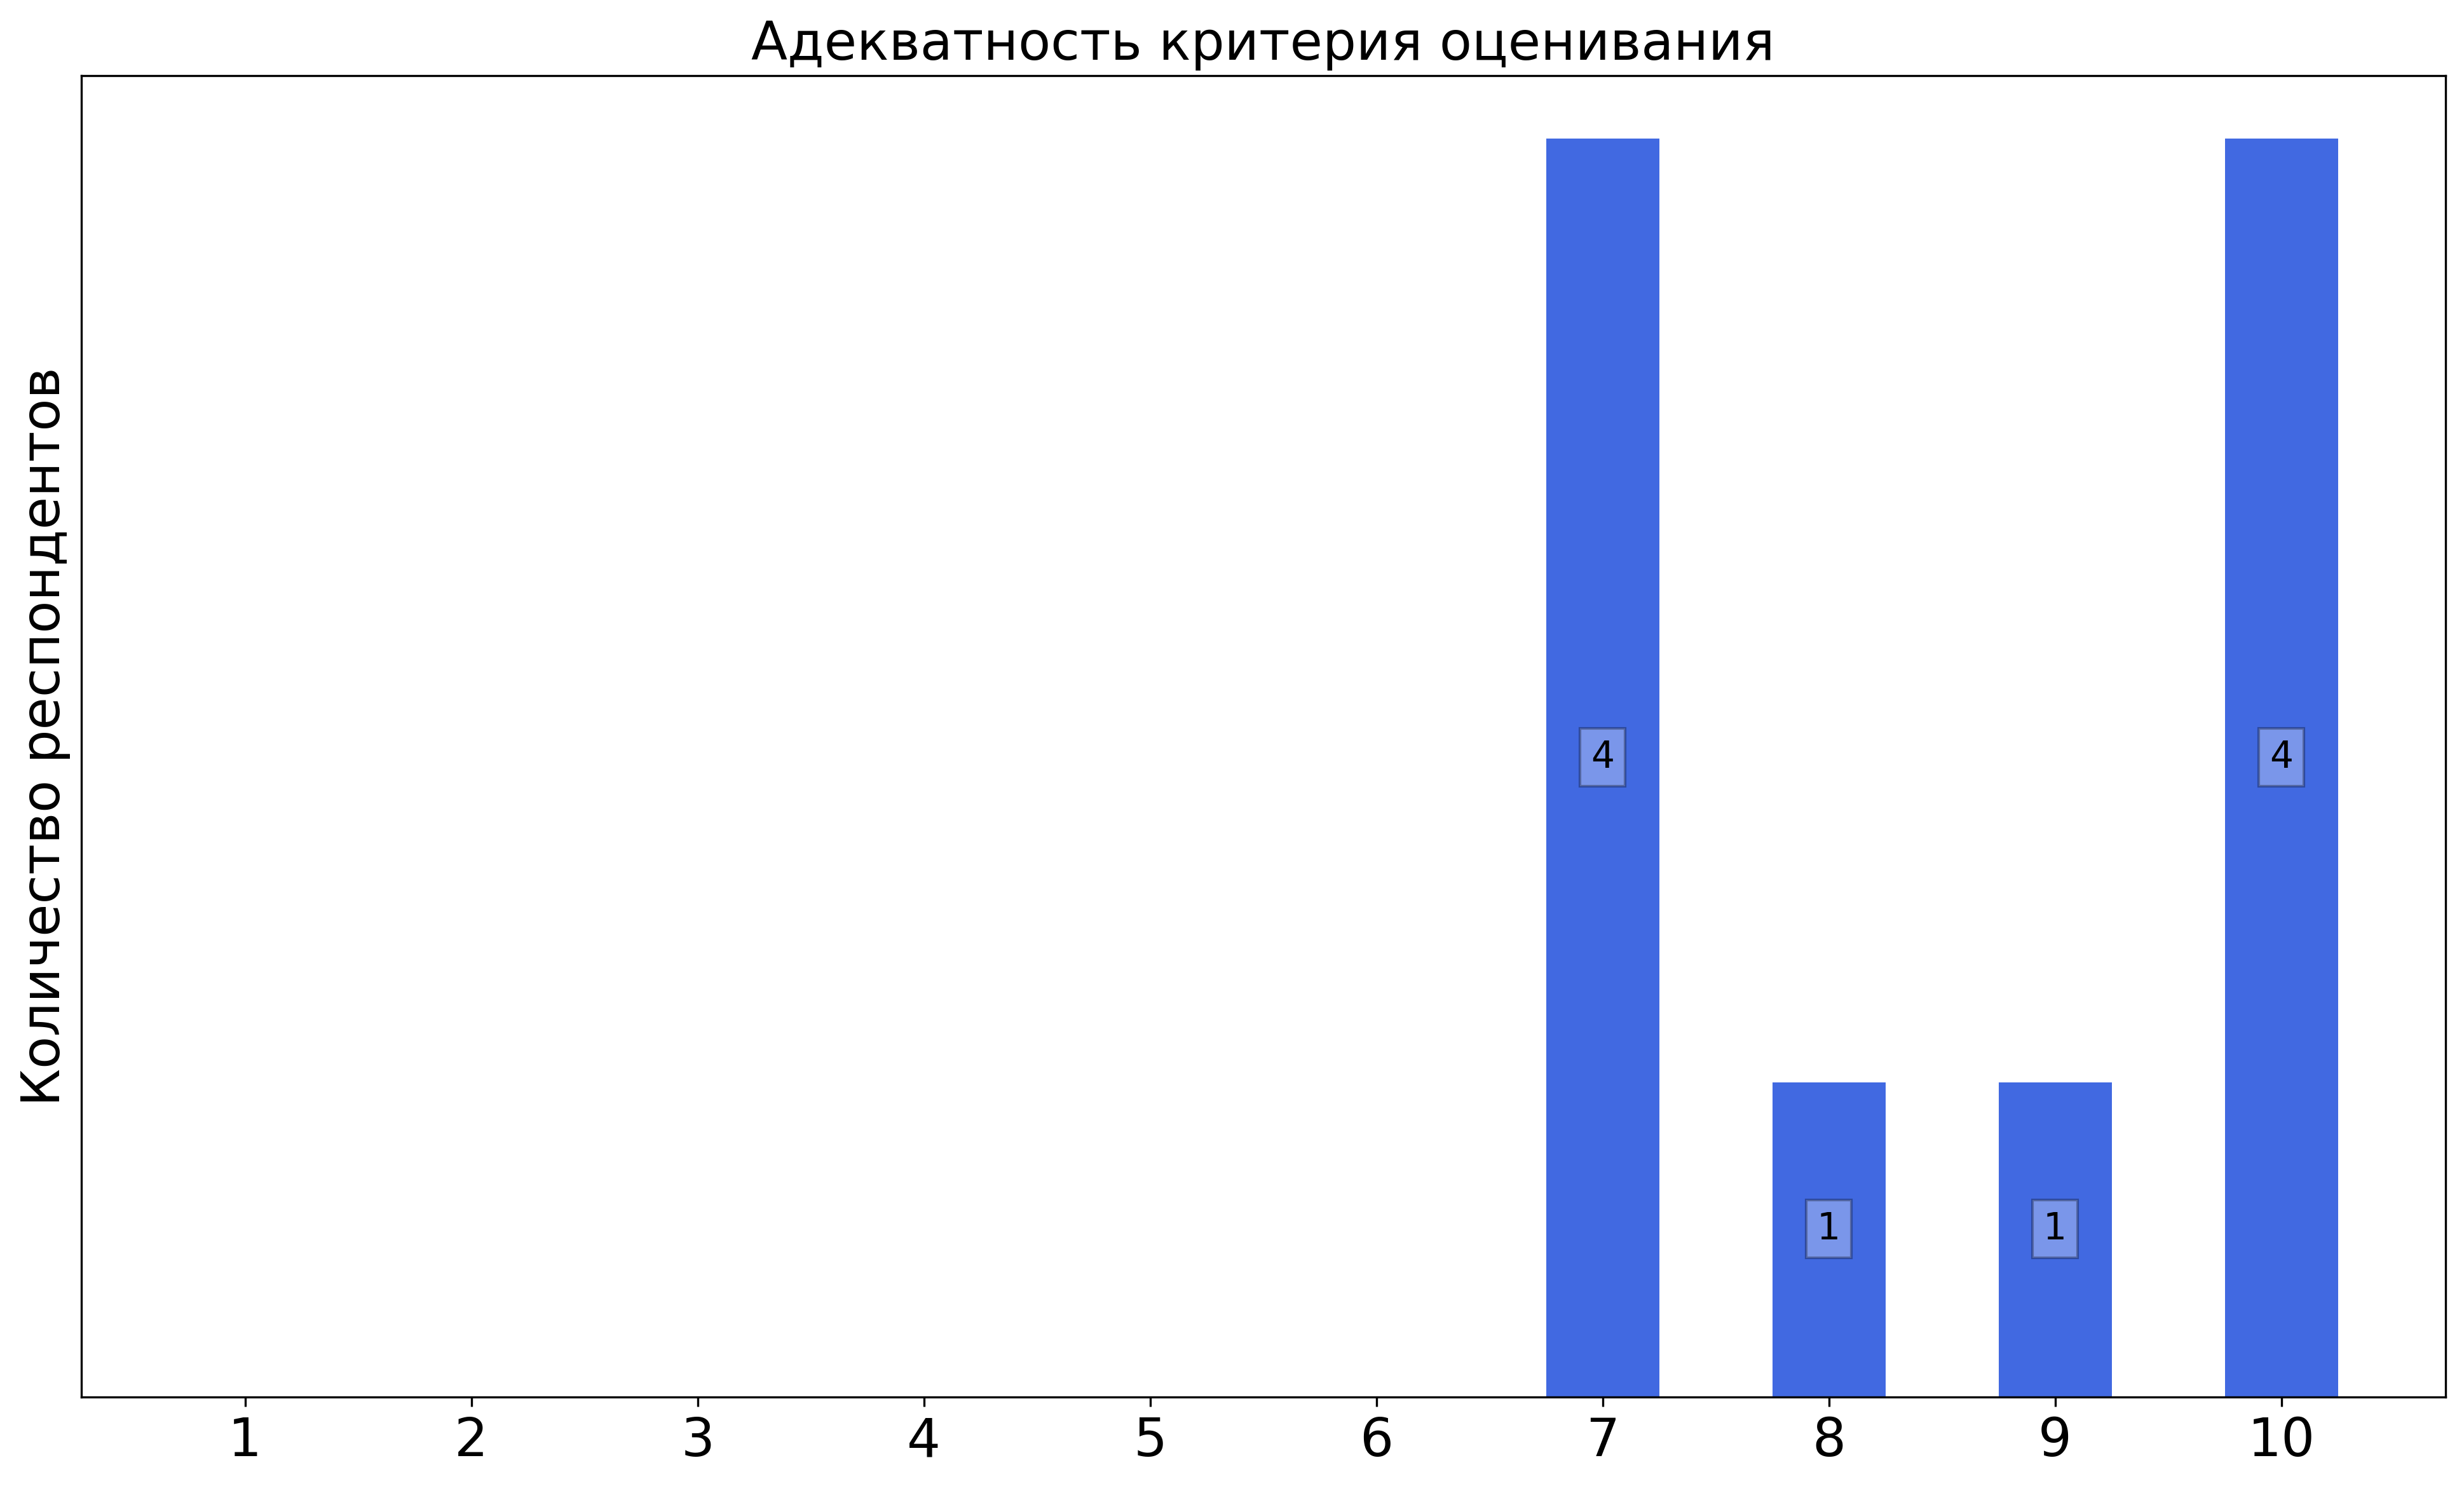
\includegraphics[width=\textwidth]{images/3 course/Аналоговая электроника/labniks-marks-Зарипов Р.А.-1.png}
			\end{subfigure}
			\begin{subfigure}[b]{0.45\textwidth}
				\centering
				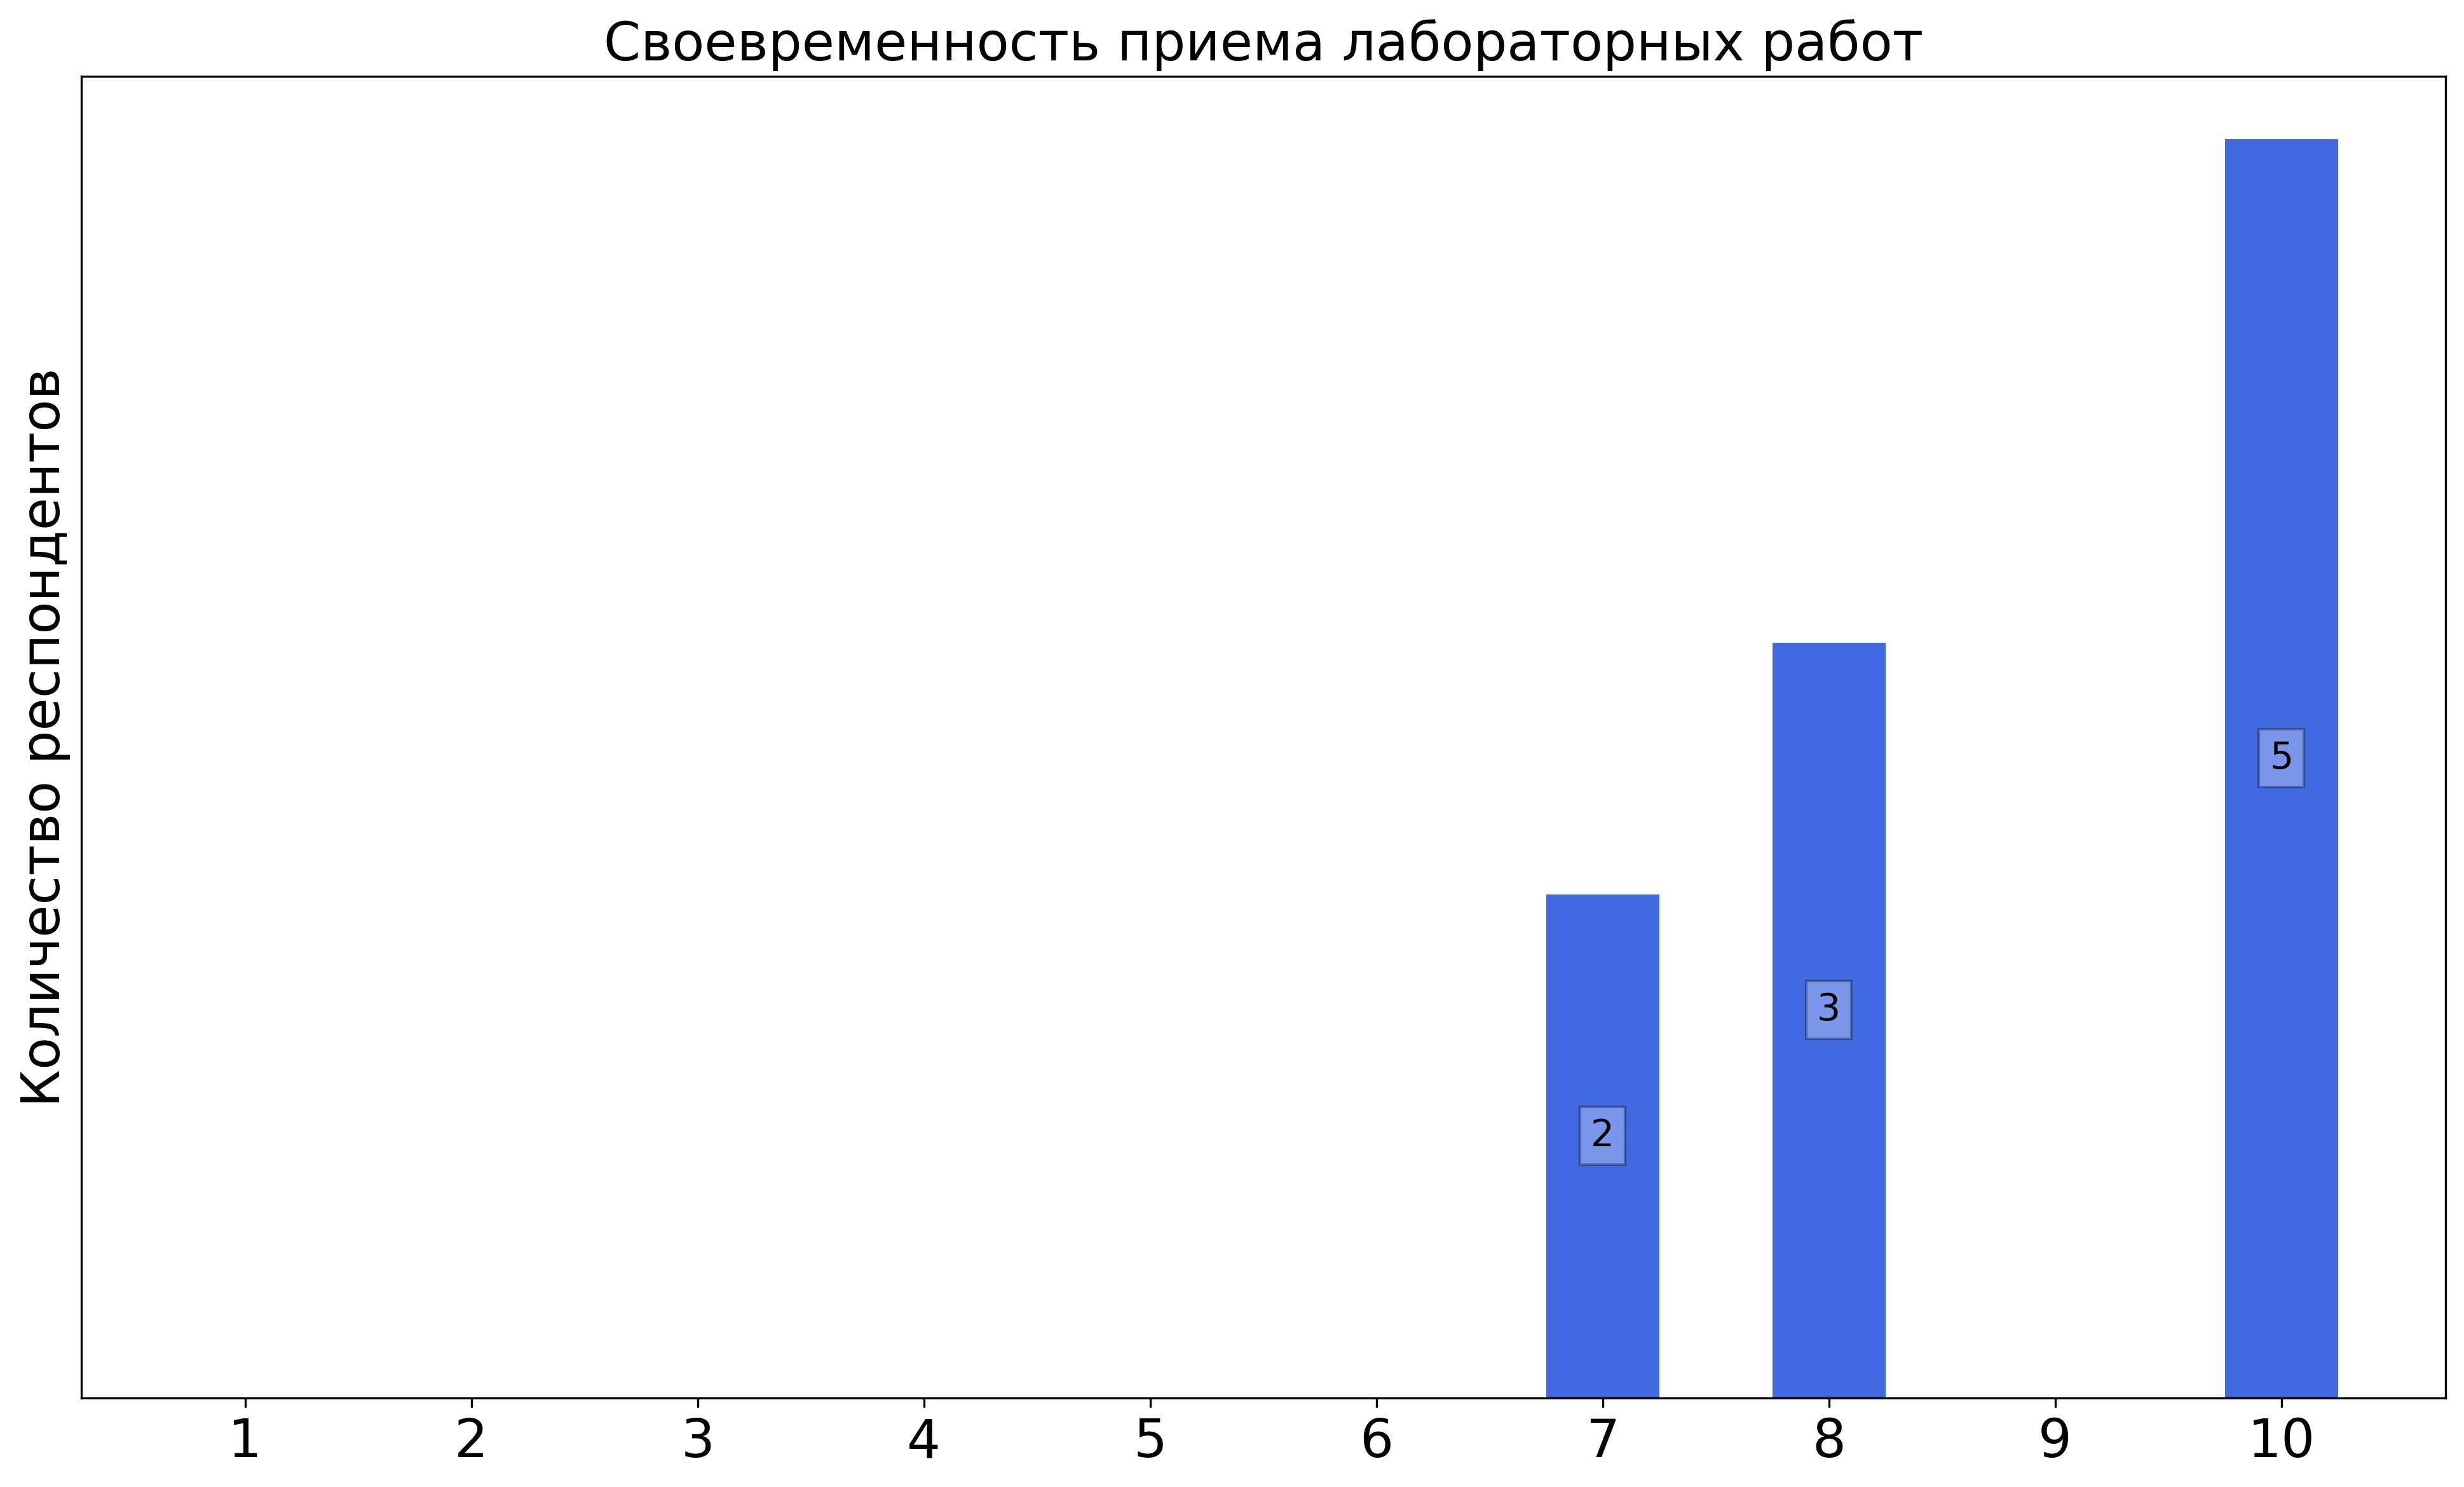
\includegraphics[width=\textwidth]{images/3 course/Аналоговая электроника/labniks-marks-Зарипов Р.А.-2.png}
			\end{subfigure}
			\begin{subfigure}[b]{0.45\textwidth}
				\centering
				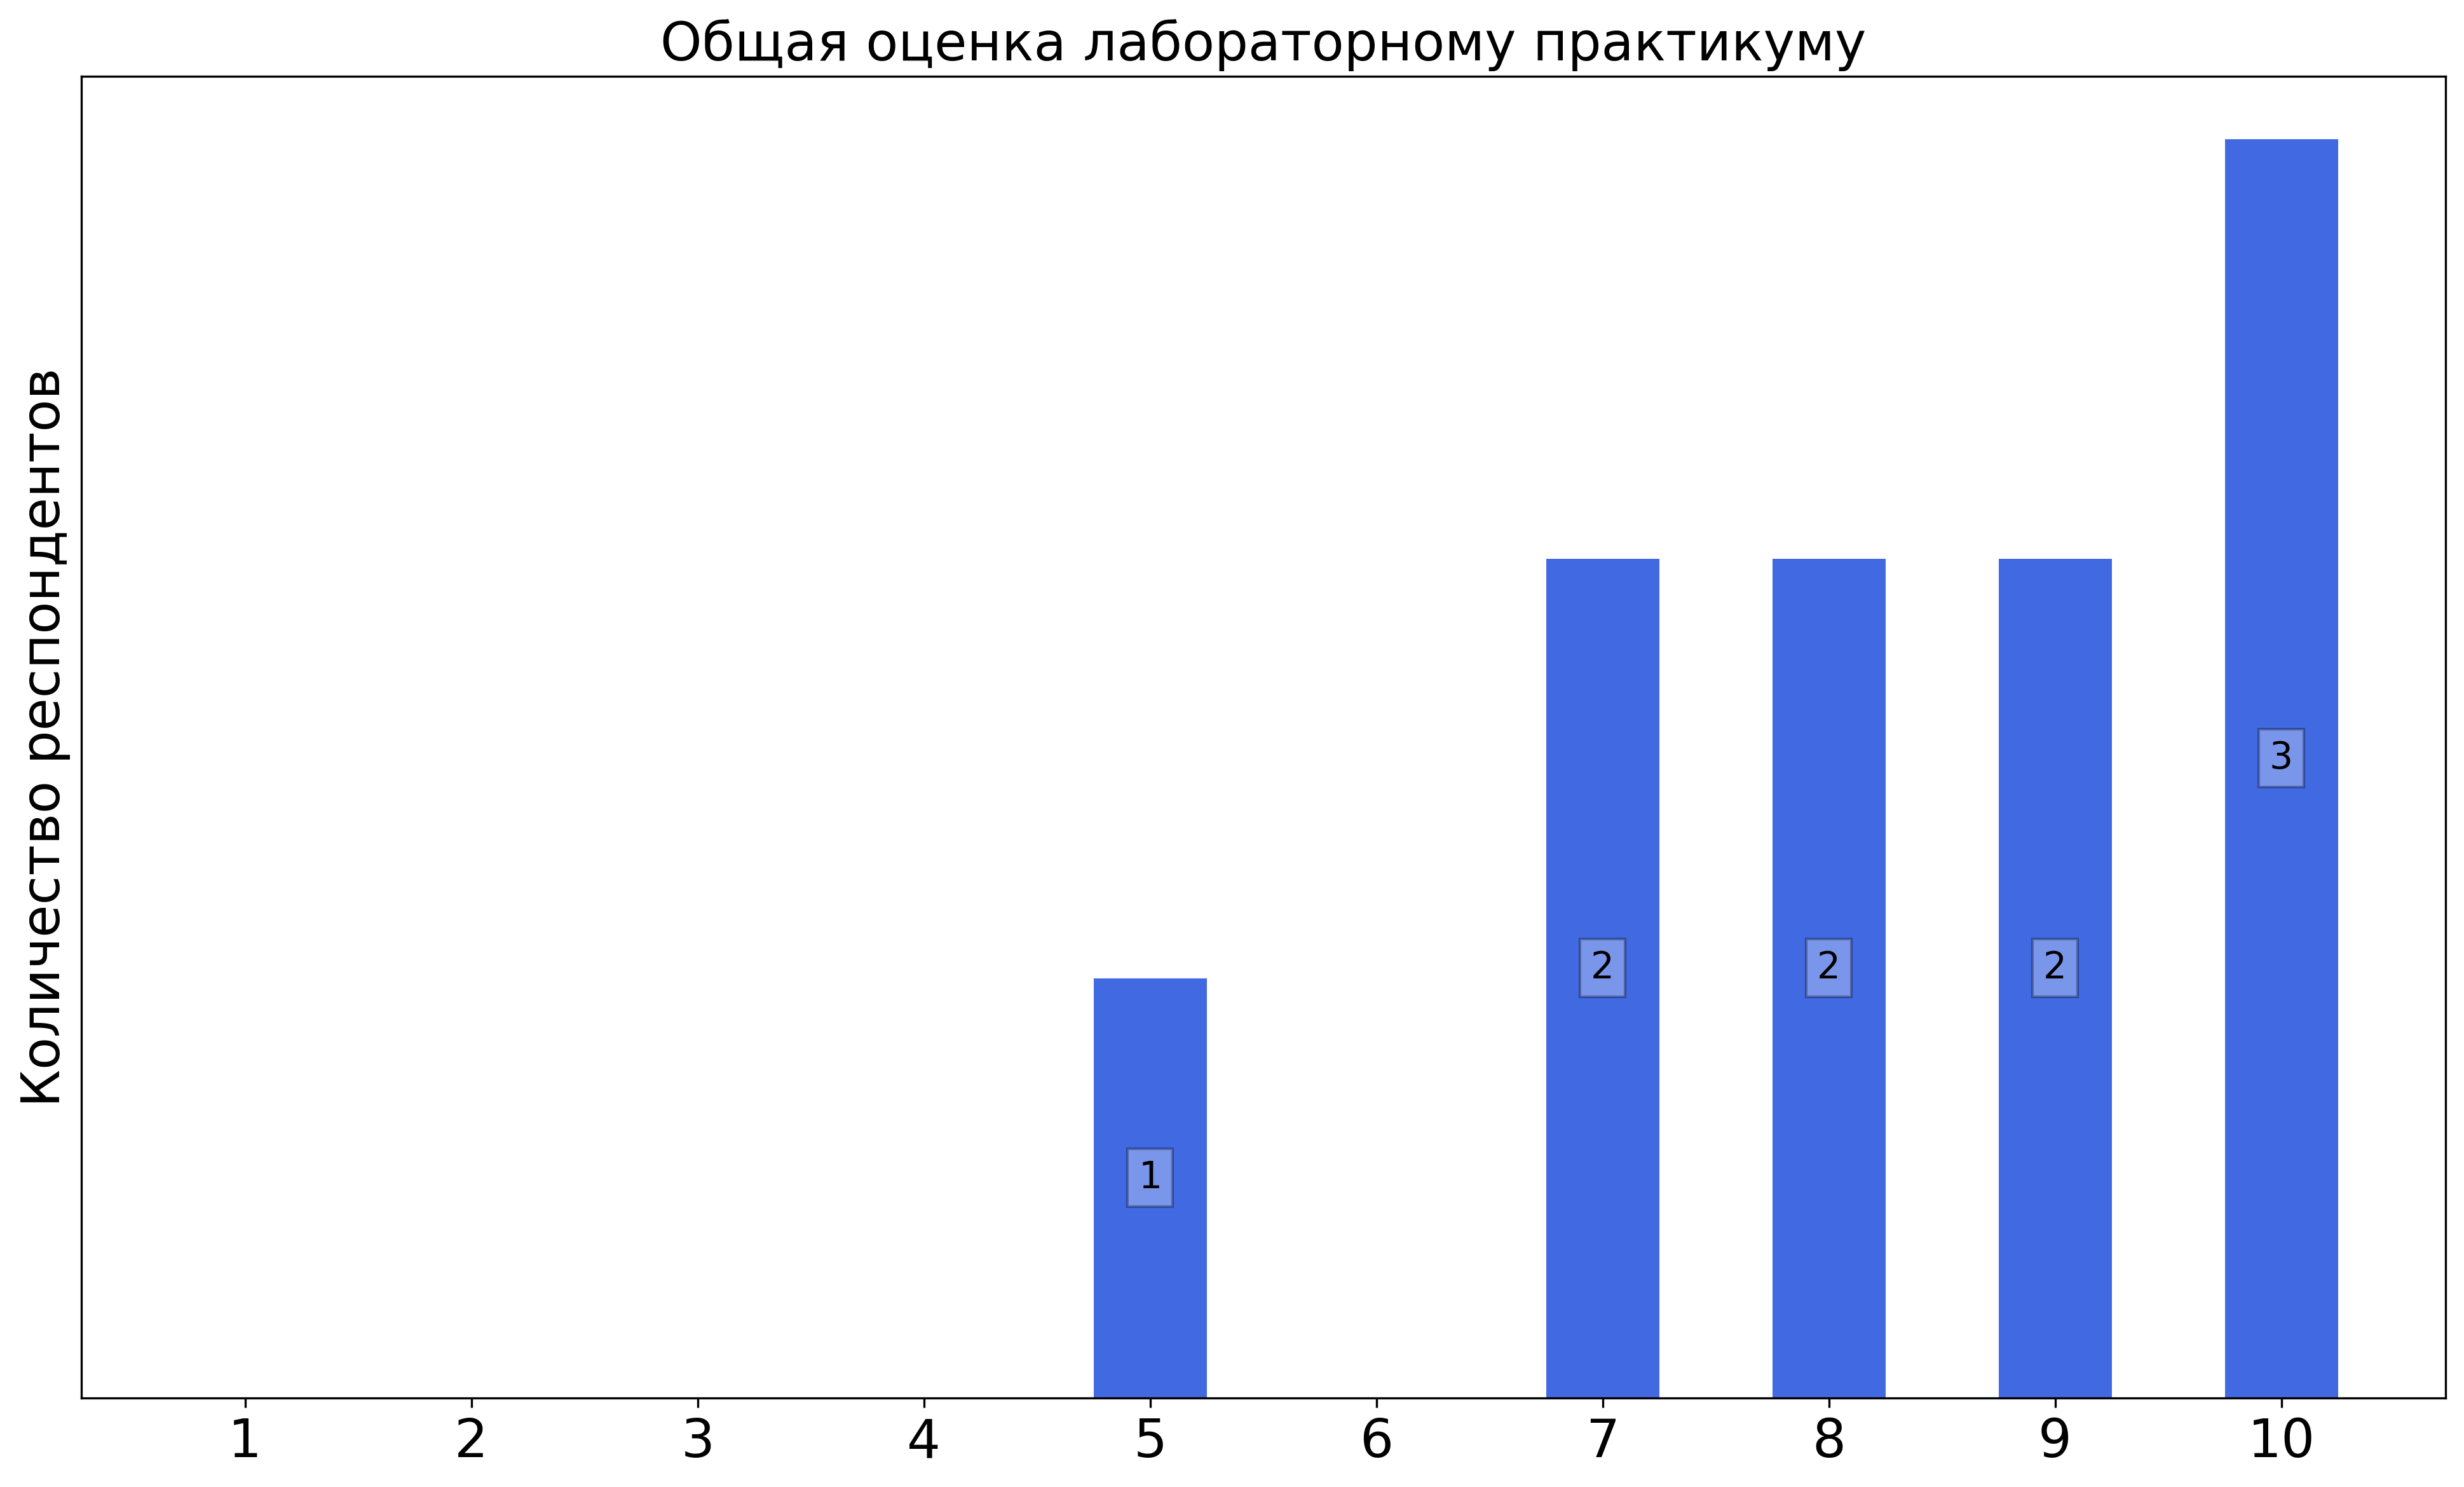
\includegraphics[width=\textwidth]{images/3 course/Аналоговая электроника/labniks-marks-Зарипов Р.А.-3.png}
			\end{subfigure}	
			\caption{Оценки респондентов о качестве преподавания лабораторных работ}
		\end{figure}

		\textbf{Комментарии студентов о преподавателе\protect\footnote{сохранены оригинальные орфография и пунктуация}}
            \begin{commentbox} 
                Преподавателю интересен его предмет, а мне нет. Из-за этого сдачи лаб были неприятные и долгие. В голове была каша и непонятно было, что я должен сделать на лабораторке. Лаба стояла рано утром, часто приходилось ботать ещё до пения петухов, чтобы кое-как получить хор 7 на сдаче 
            \end{commentbox} 
        
            \begin{commentbox} 
                Замечательный семинарист, если бы не его мини-лекции перед лабораторными работами, знаний после данного семестра не было бы никаких. Всё адекватно! 
            \end{commentbox} 
        
            \begin{commentbox} 
                Преподаватель, к которому перевёлся очень понравился, некоторые темы лабараторных + качество некоторого оьорудования в лабаратории не очень понравились, иногда работали на неработающих установках (платах/неработающих компонентах) 
            \end{commentbox} 
        
            \begin{commentbox} 
                Зарипов лапочка, сам практикум не самый интересный, но если разбираться, то прикольно. 
            \end{commentbox} 
        
            \begin{commentbox} 
                Очень понравилось, разобралась в предмете 
            \end{commentbox} 
        
            \begin{commentbox} 
                Хоть Руслан и пытался объяснять что-то, скидывал материалы и на сдачах спрашивал довольно подробно, после курса понимания не сложилось никакого. Я пыталась понять, смотрела лекции и закрыла на 8, но ничего не осталось в голове. 
            \end{commentbox} 


    \subsubsection{Отзыв студентов о лабораторных работах. Преподаватель: Иващенко А.А.}
		\begin{figure}[H]
			\centering
			\begin{subfigure}[b]{0.45\textwidth}
				\centering
				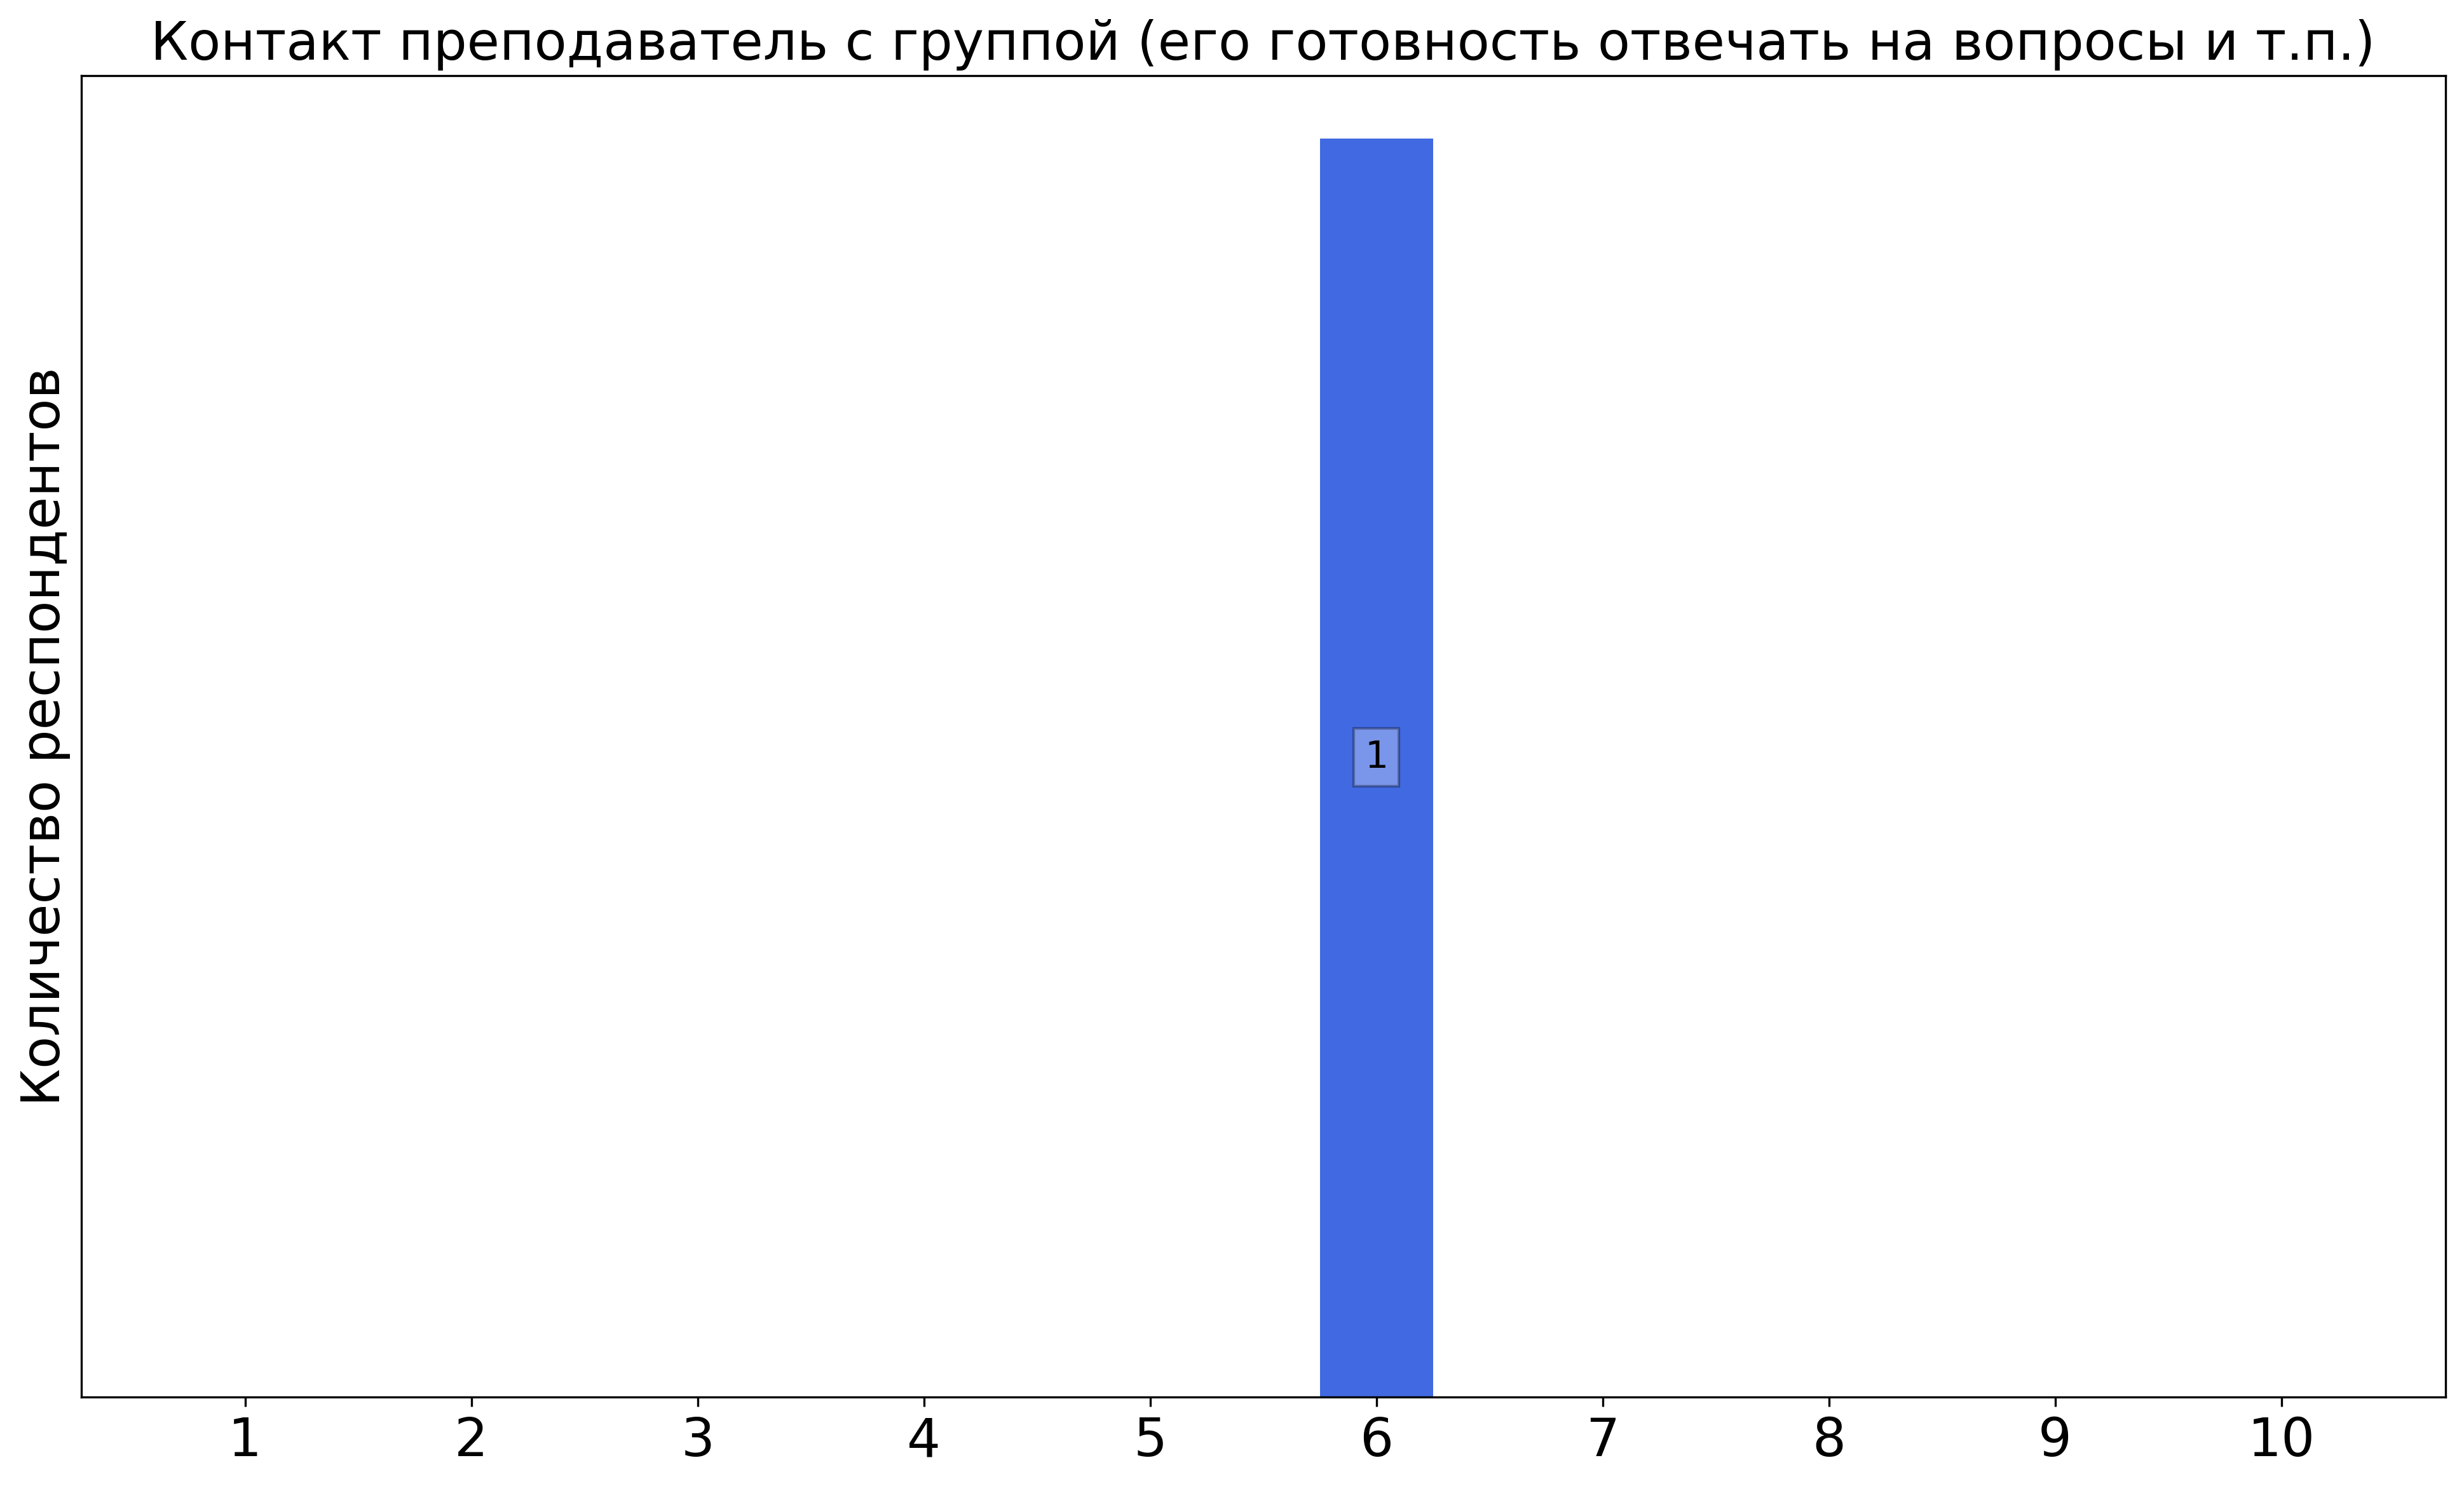
\includegraphics[width=\textwidth]{images/3 course/Аналоговая электроника/labniks-marks-Иващенко А.А.-0.png}
			\end{subfigure}
			\begin{subfigure}[b]{0.45\textwidth}
				\centering
				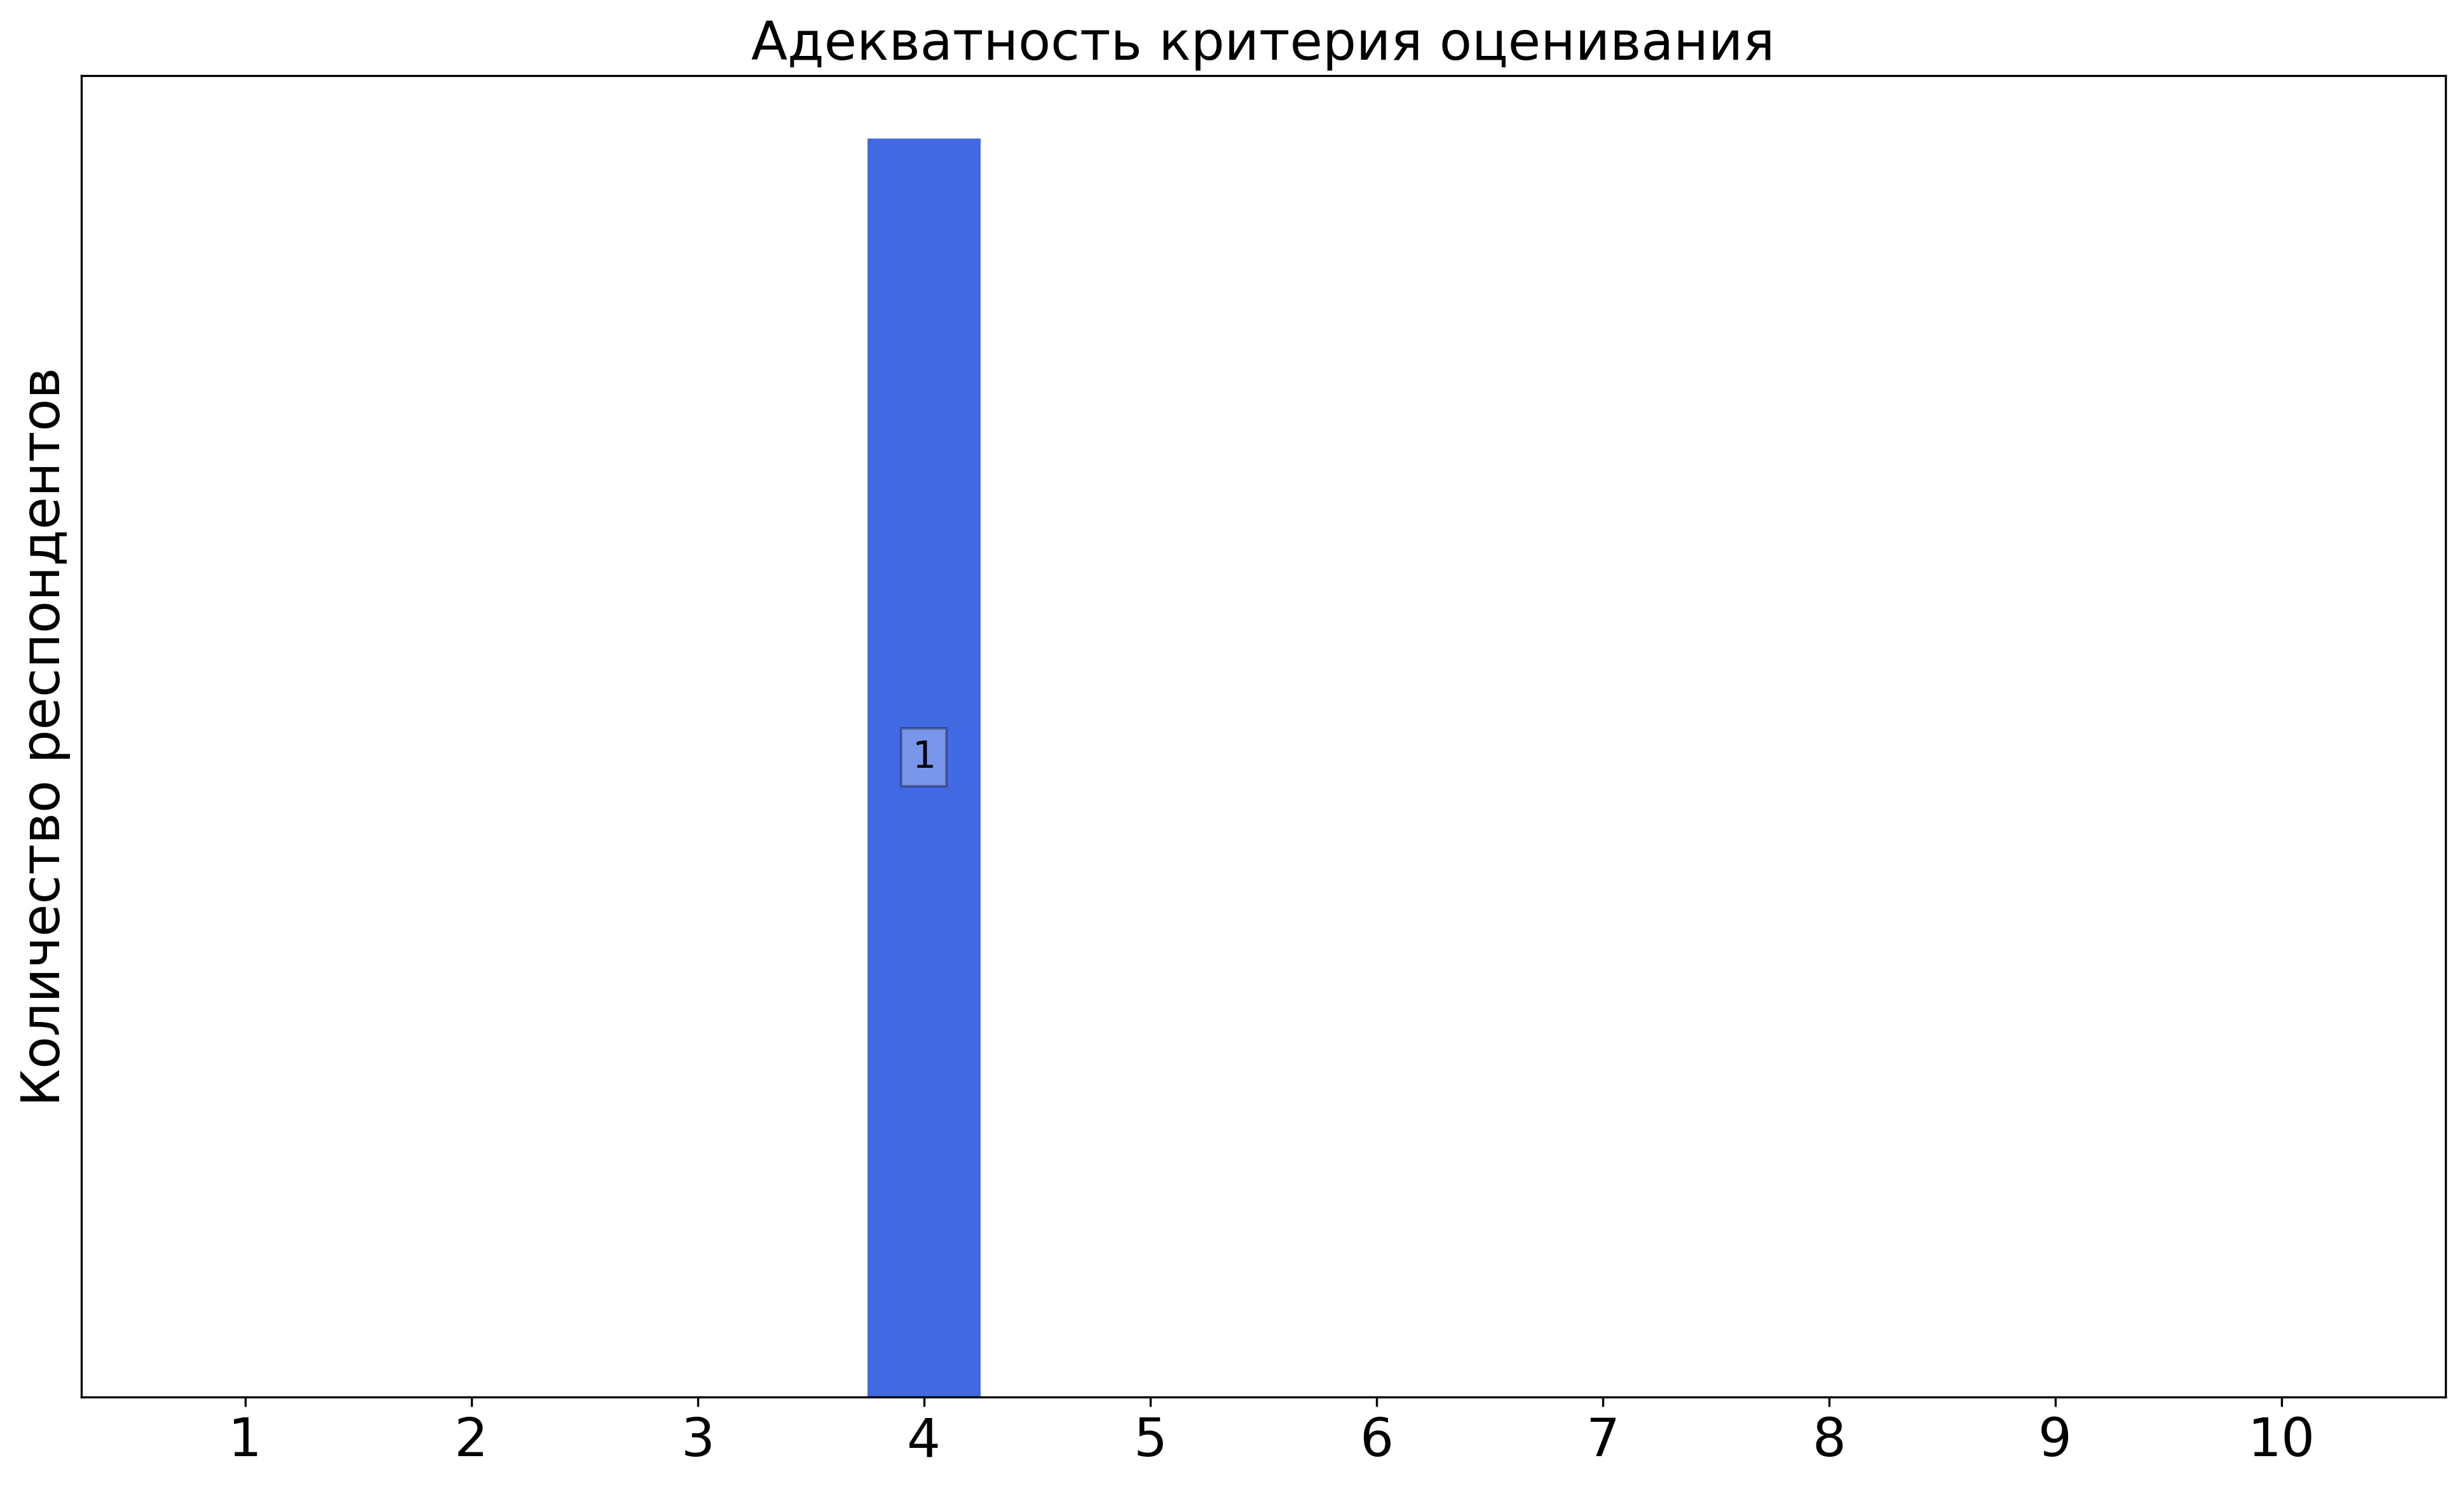
\includegraphics[width=\textwidth]{images/3 course/Аналоговая электроника/labniks-marks-Иващенко А.А.-1.png}
			\end{subfigure}
			\begin{subfigure}[b]{0.45\textwidth}
				\centering
				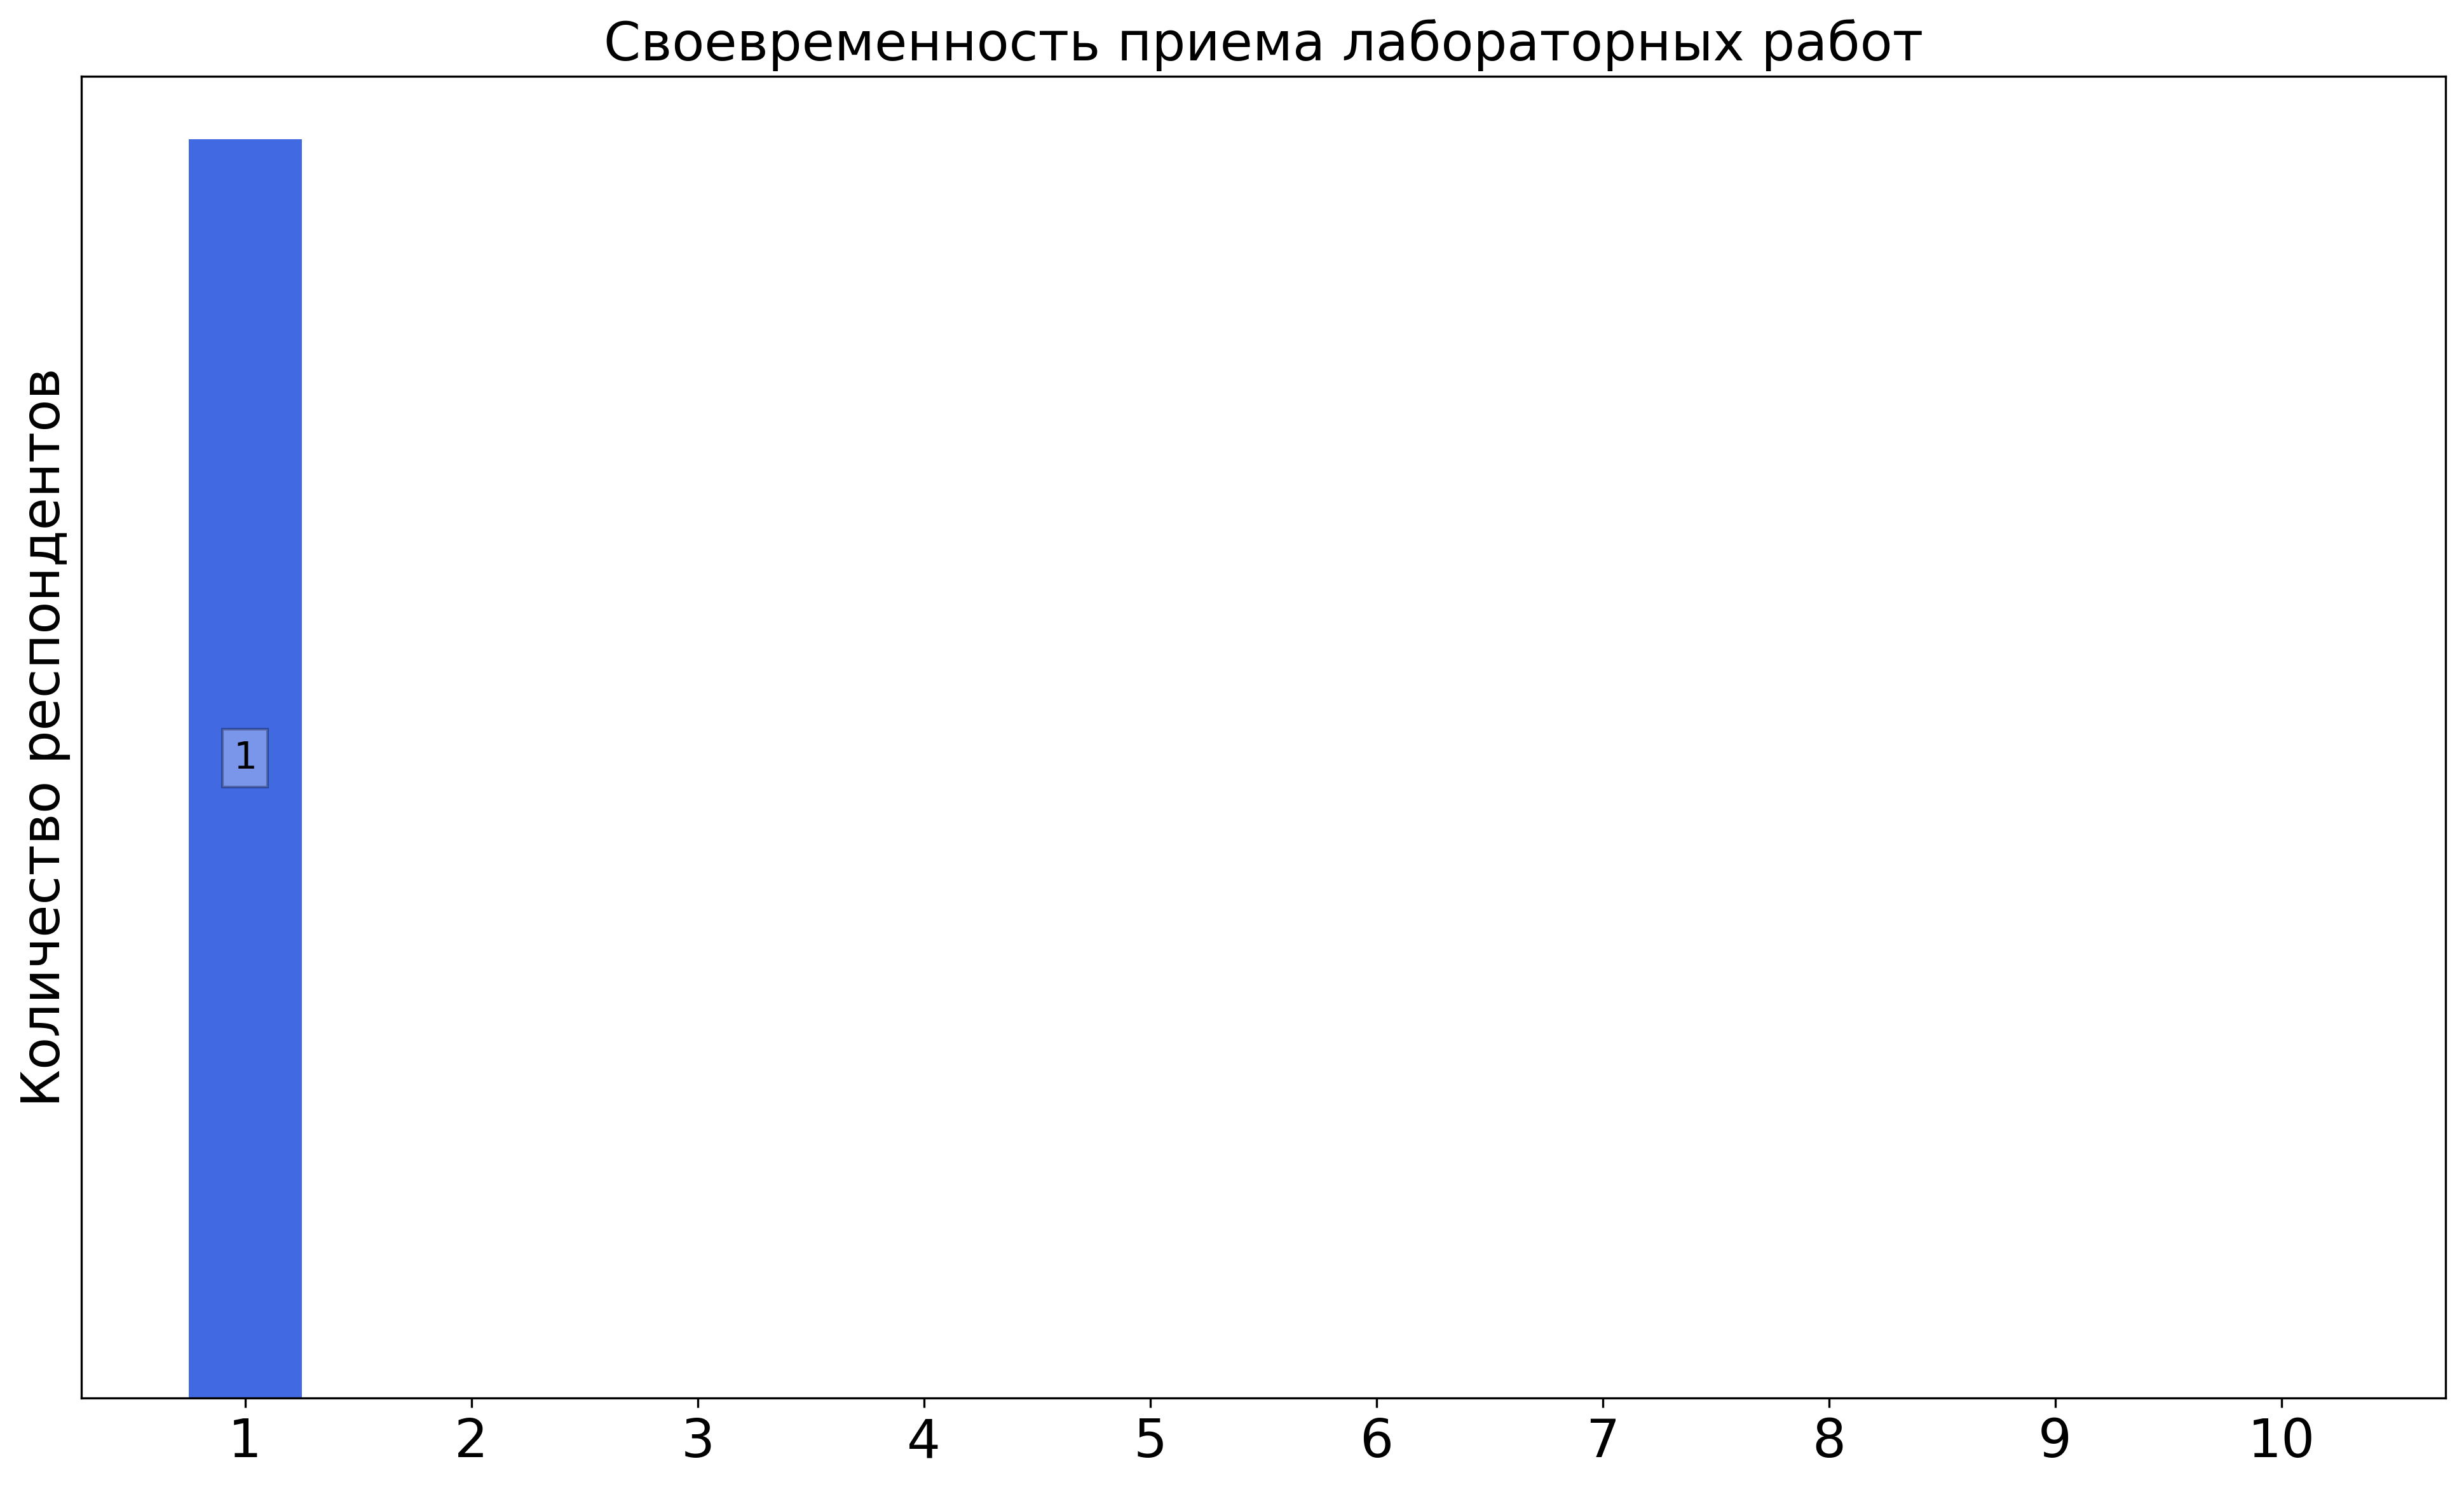
\includegraphics[width=\textwidth]{images/3 course/Аналоговая электроника/labniks-marks-Иващенко А.А.-2.png}
			\end{subfigure}
			\begin{subfigure}[b]{0.45\textwidth}
				\centering
				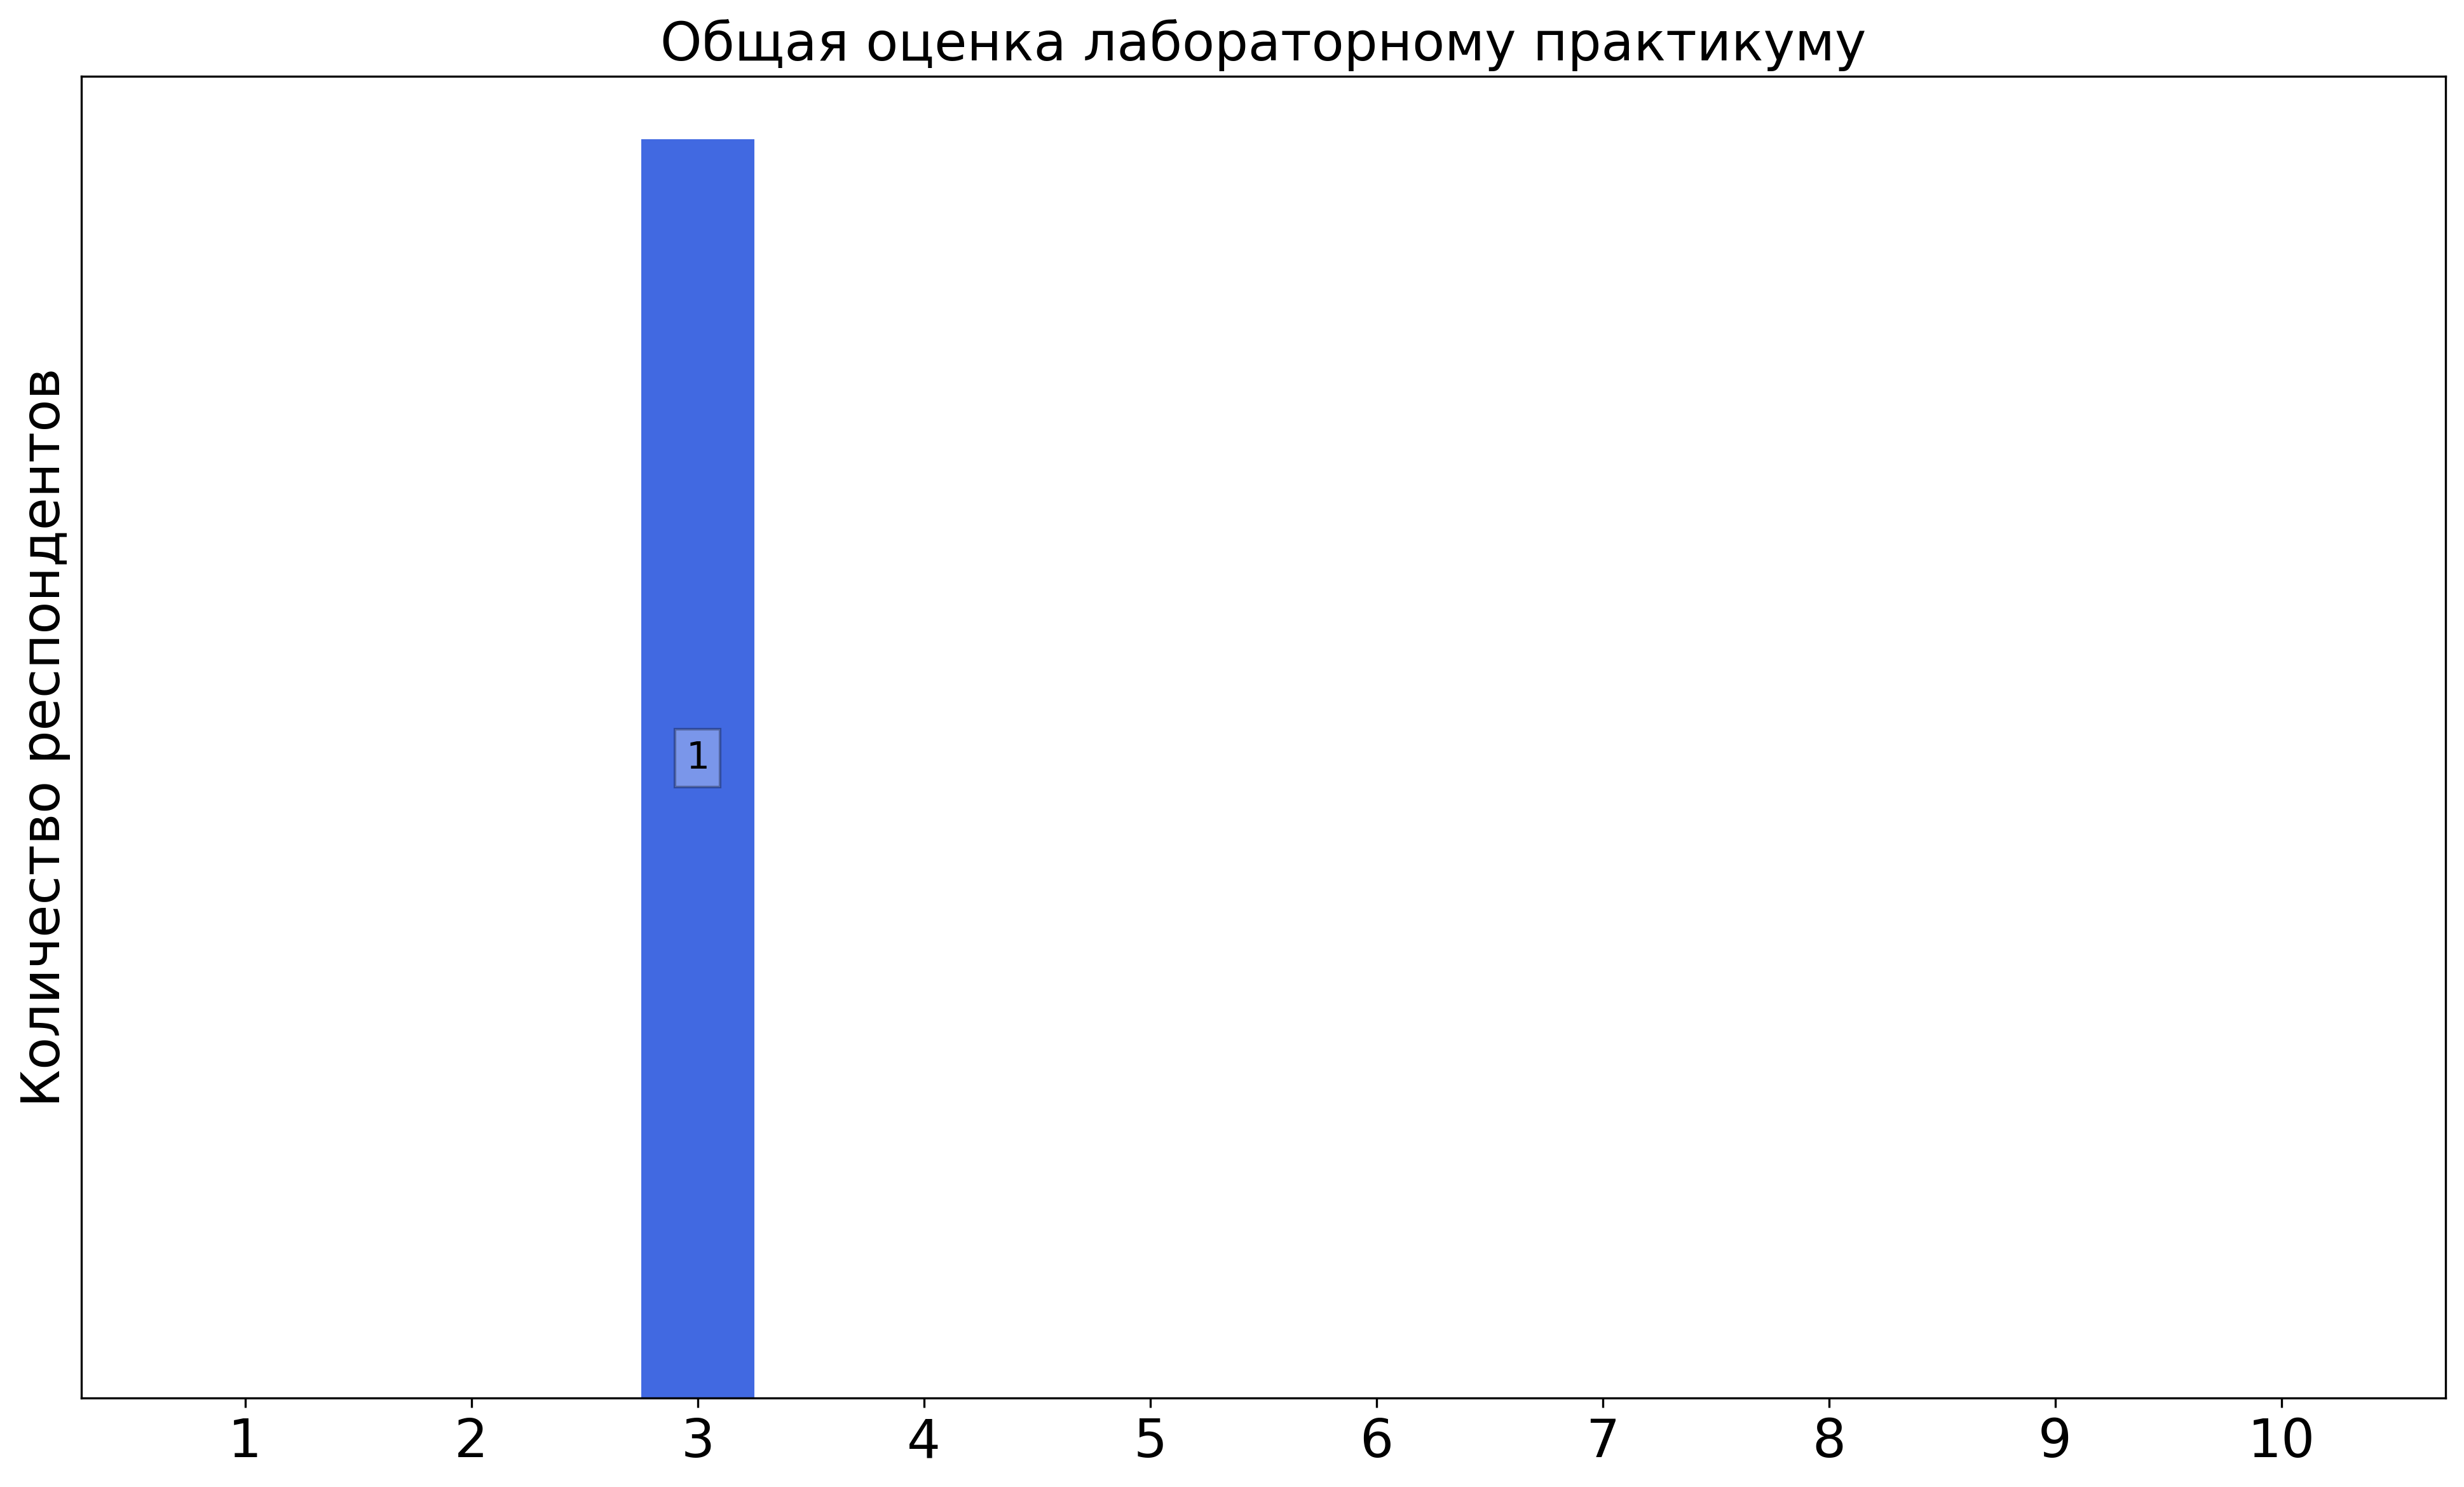
\includegraphics[width=\textwidth]{images/3 course/Аналоговая электроника/labniks-marks-Иващенко А.А.-3.png}
			\end{subfigure}	
			\caption{Оценки респондентов о качестве преподавания лабораторных работ}
		\end{figure}


    \subsubsection{Отзыв студентов о лабораторных работах. Преподаватель: Неешпапа А.В.}
		\begin{figure}[H]
			\centering
			\begin{subfigure}[b]{0.45\textwidth}
				\centering
				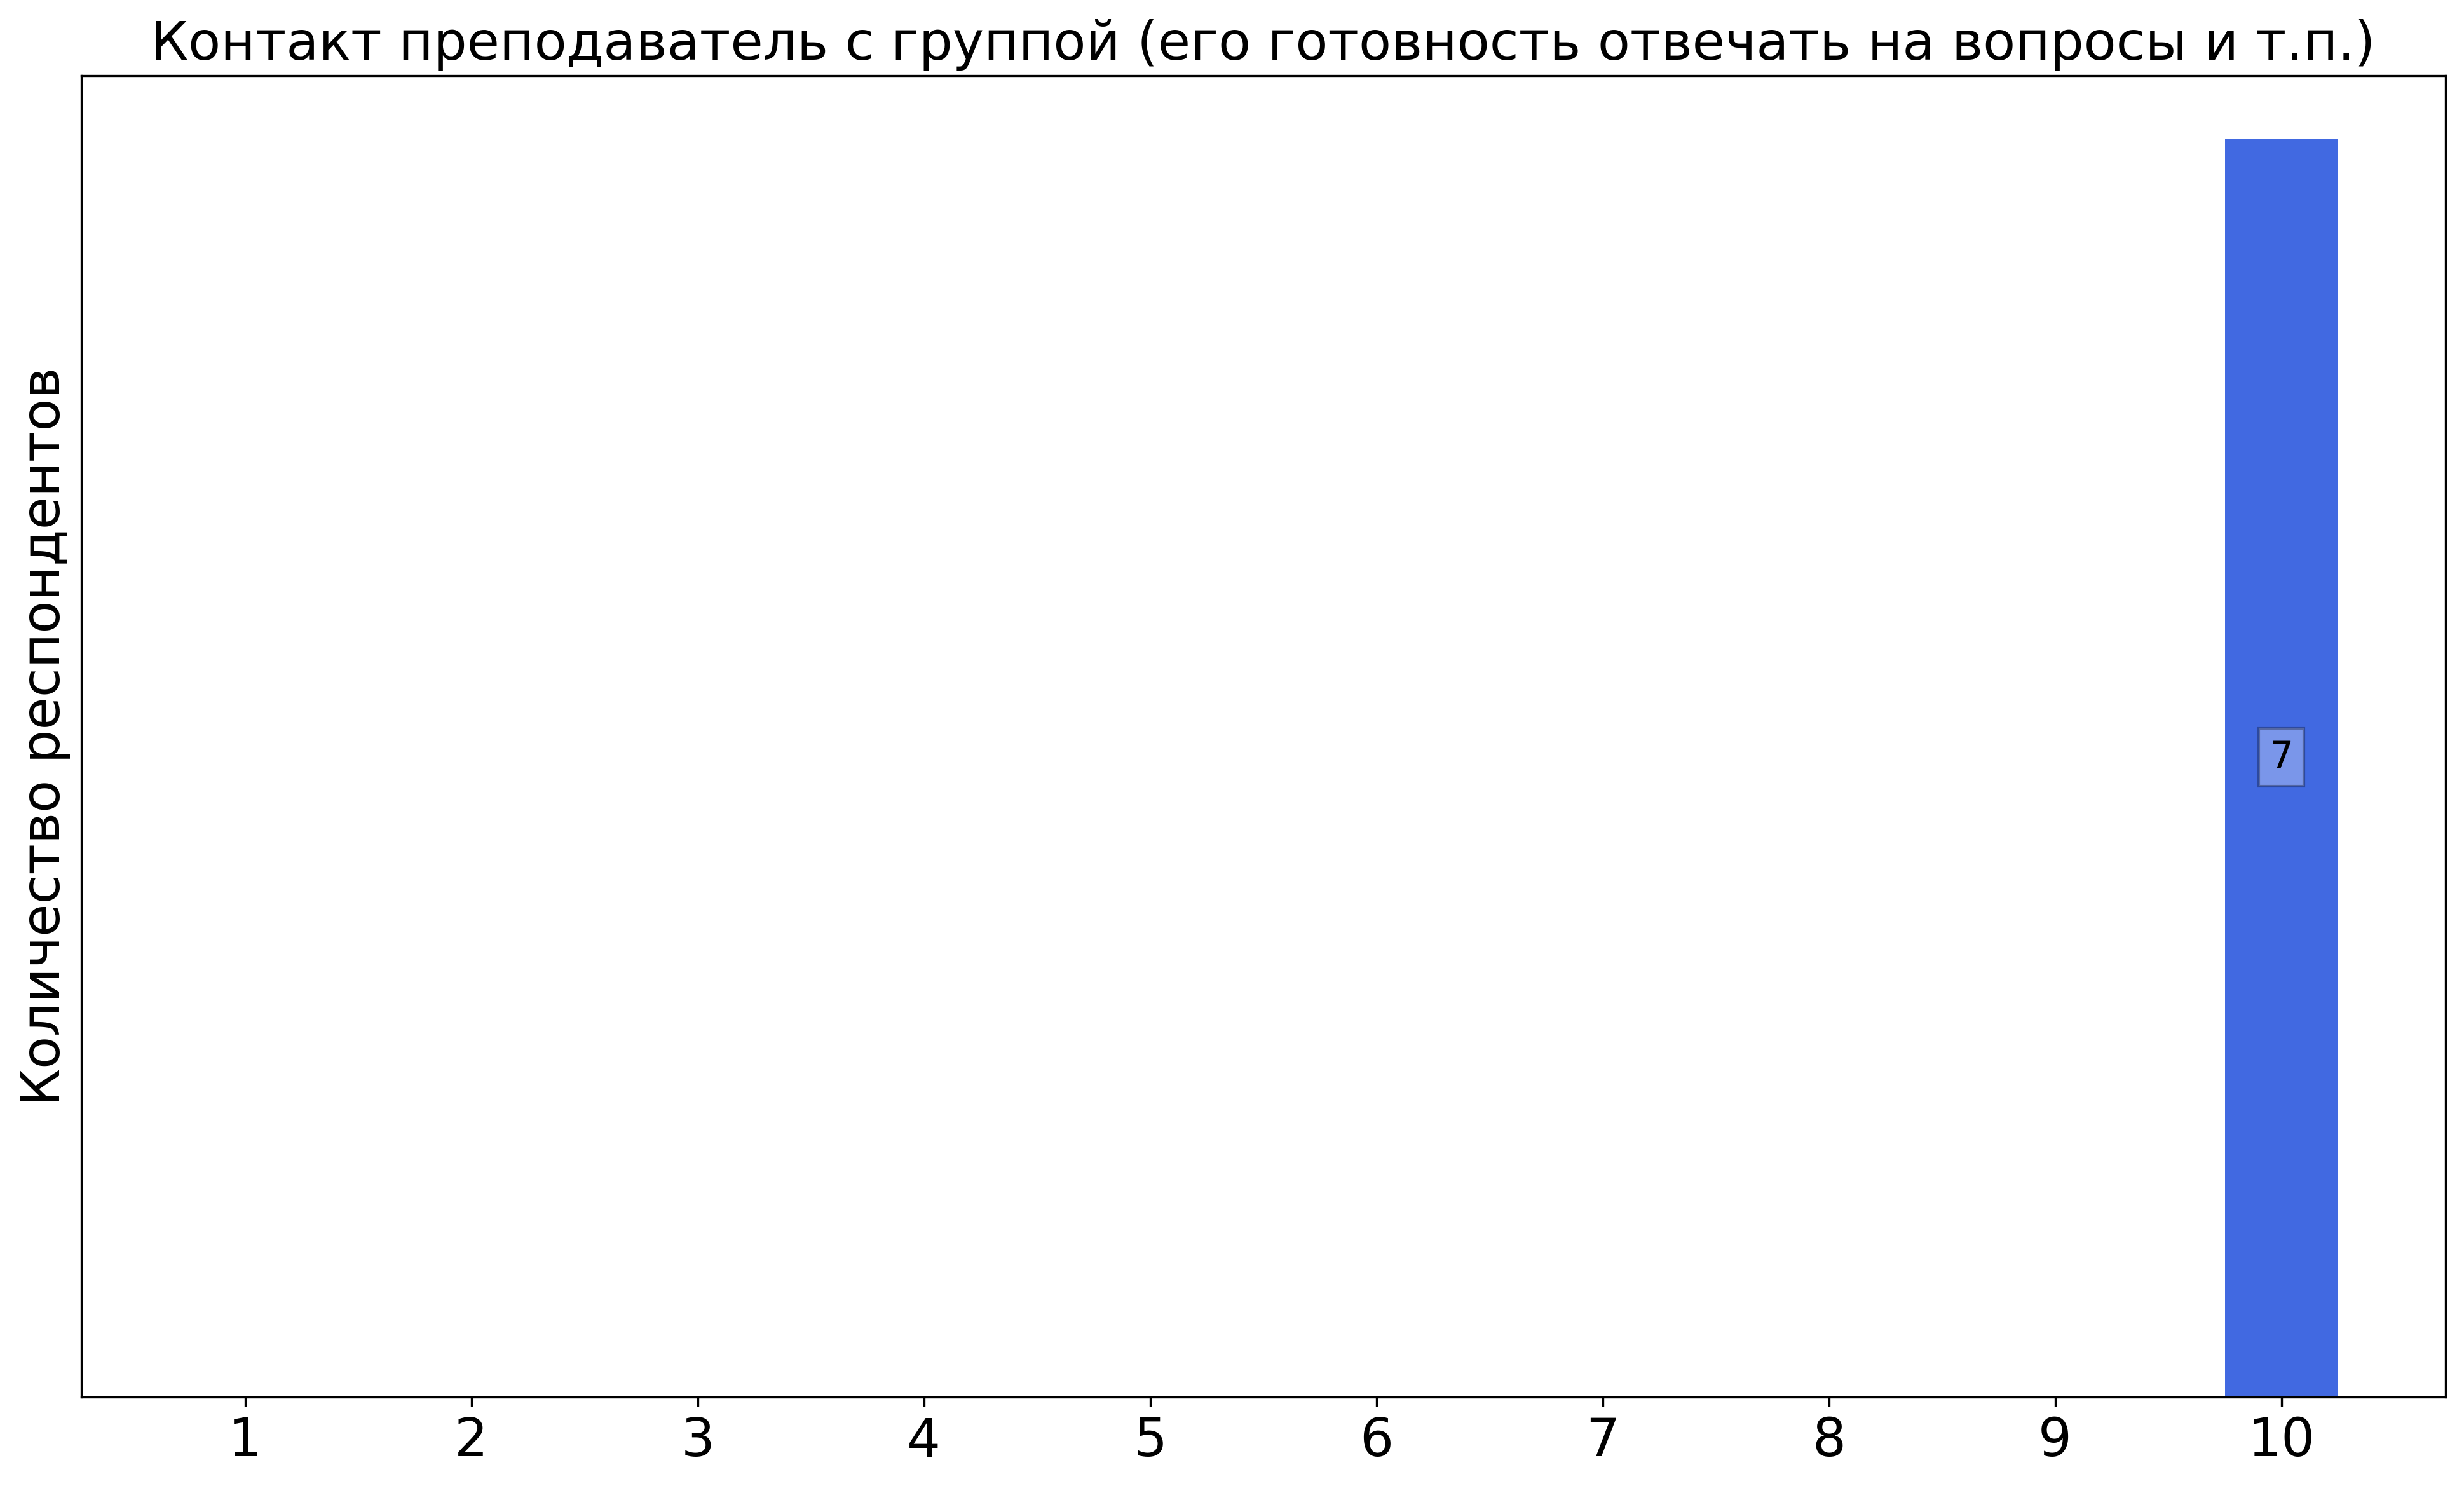
\includegraphics[width=\textwidth]{images/3 course/Аналоговая электроника/labniks-marks-Неешпапа А.В.-0.png}
			\end{subfigure}
			\begin{subfigure}[b]{0.45\textwidth}
				\centering
				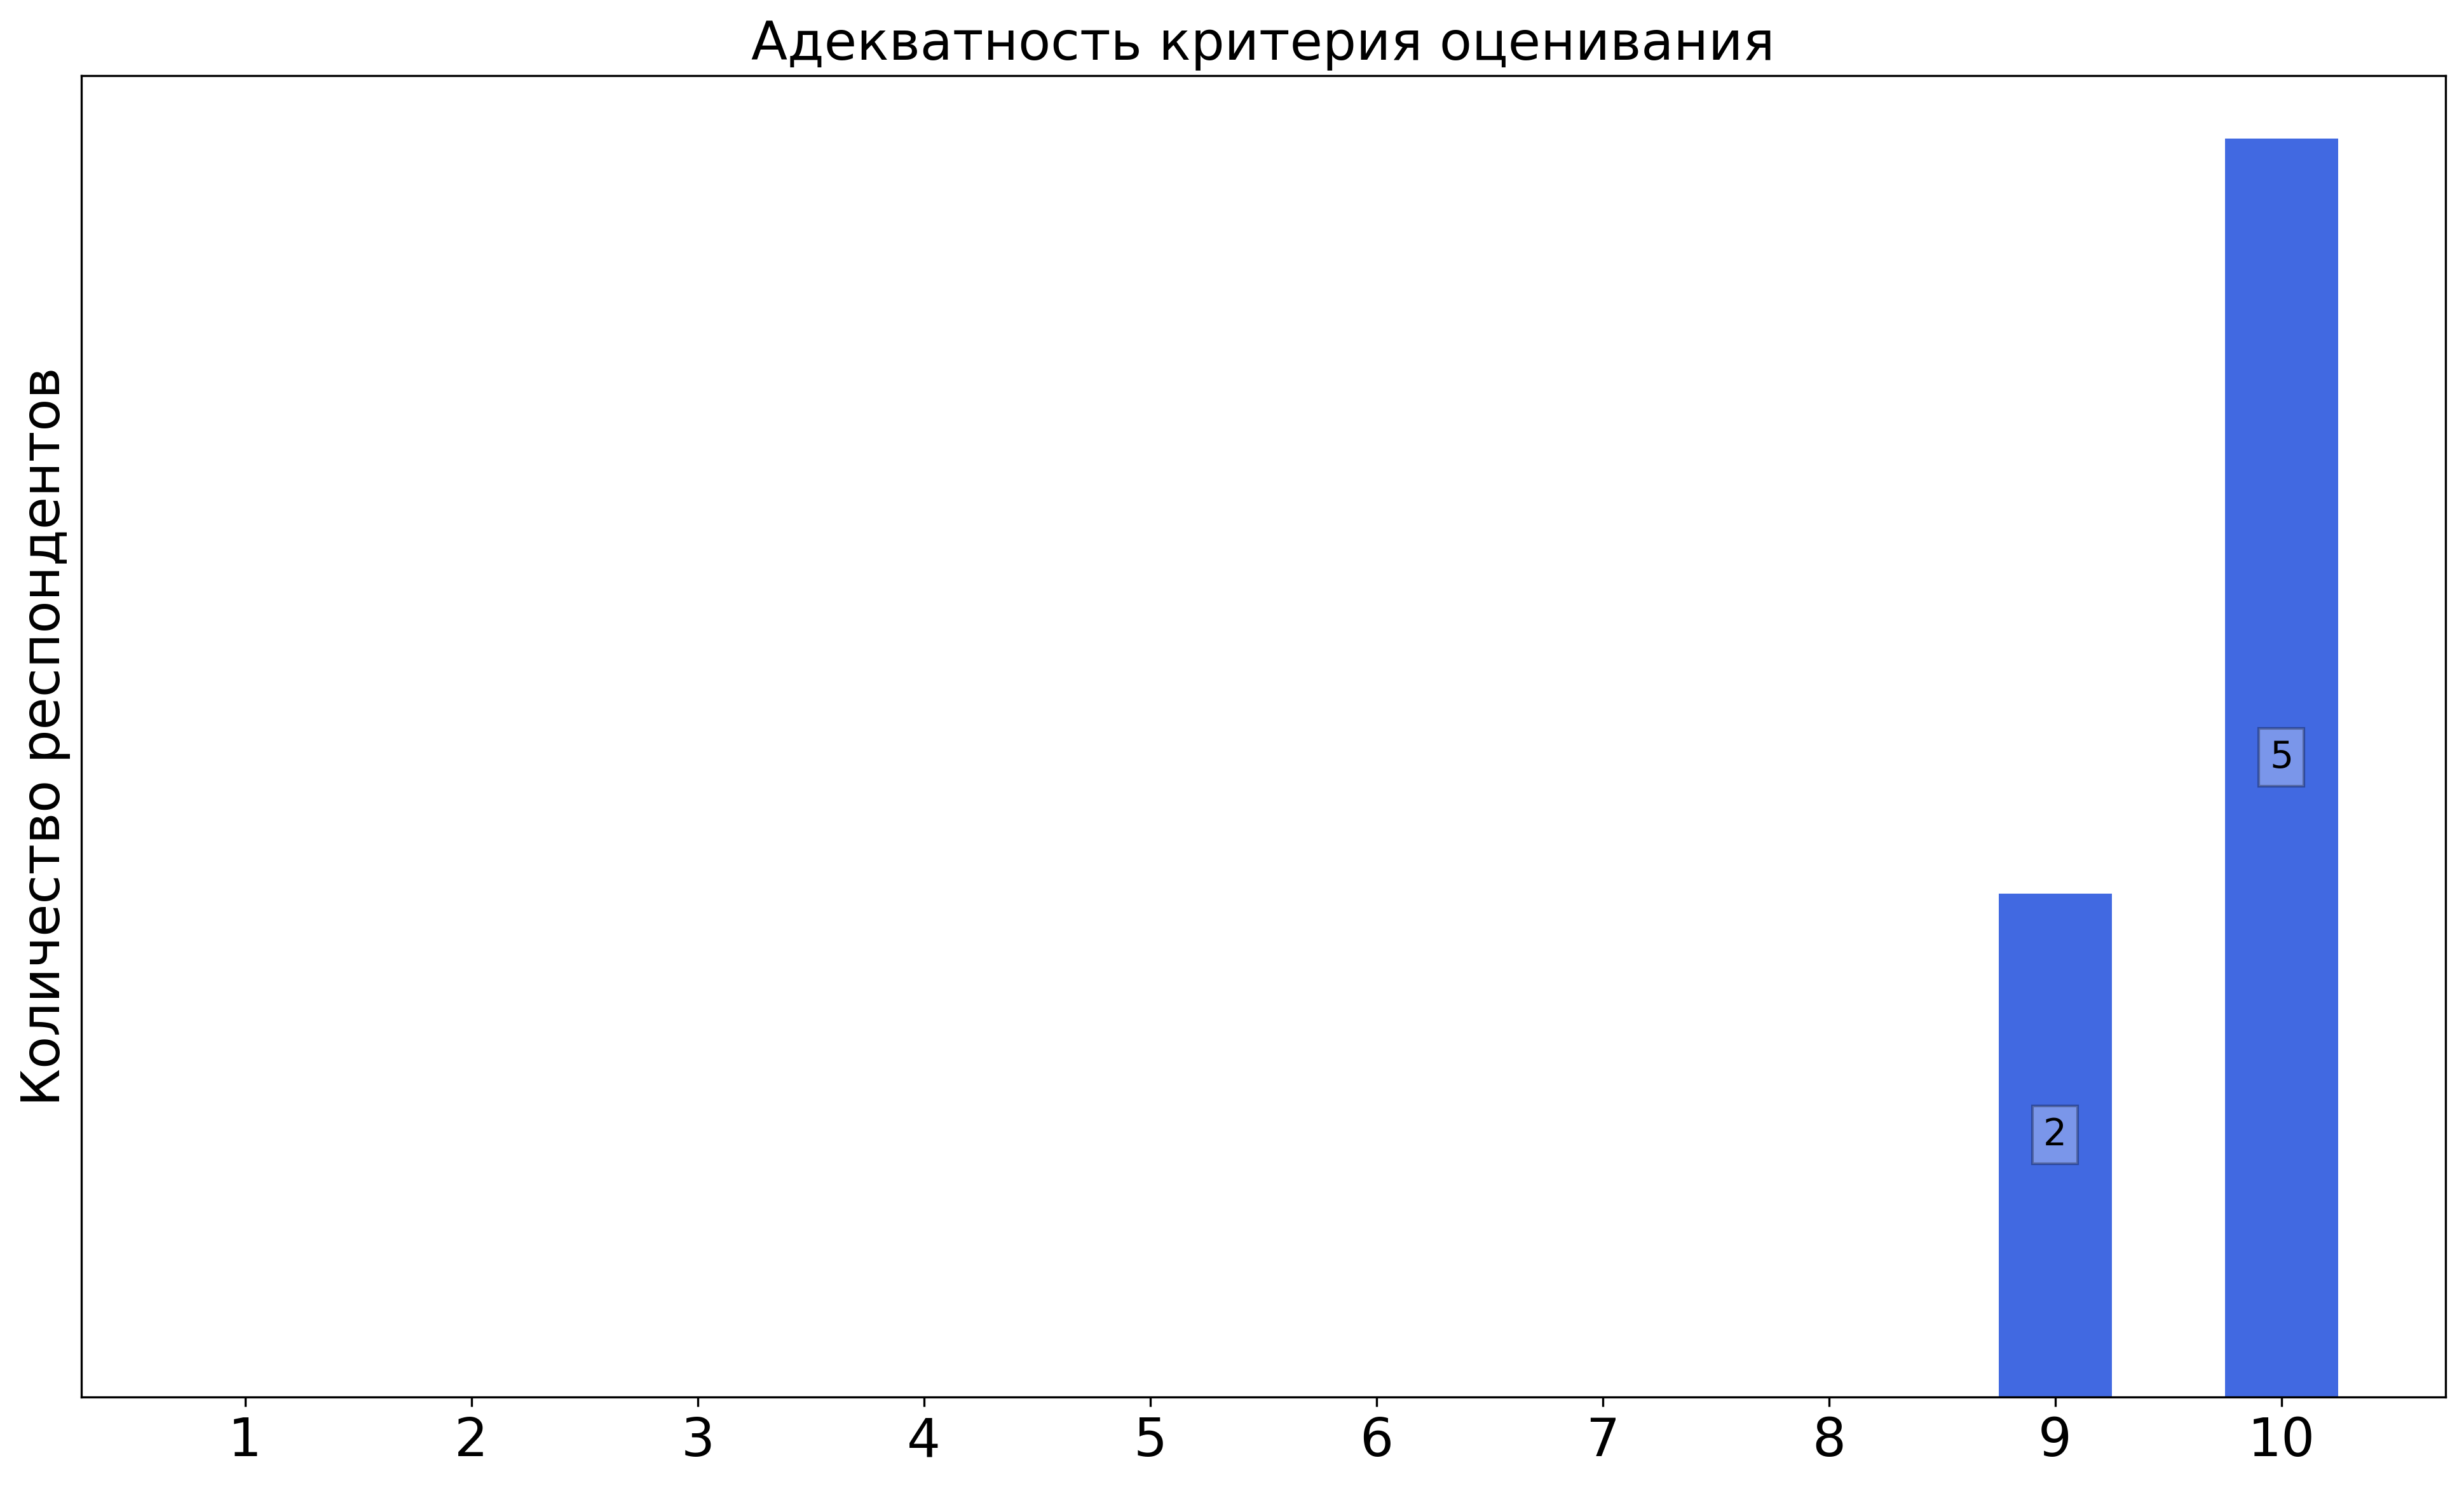
\includegraphics[width=\textwidth]{images/3 course/Аналоговая электроника/labniks-marks-Неешпапа А.В.-1.png}
			\end{subfigure}
			\begin{subfigure}[b]{0.45\textwidth}
				\centering
				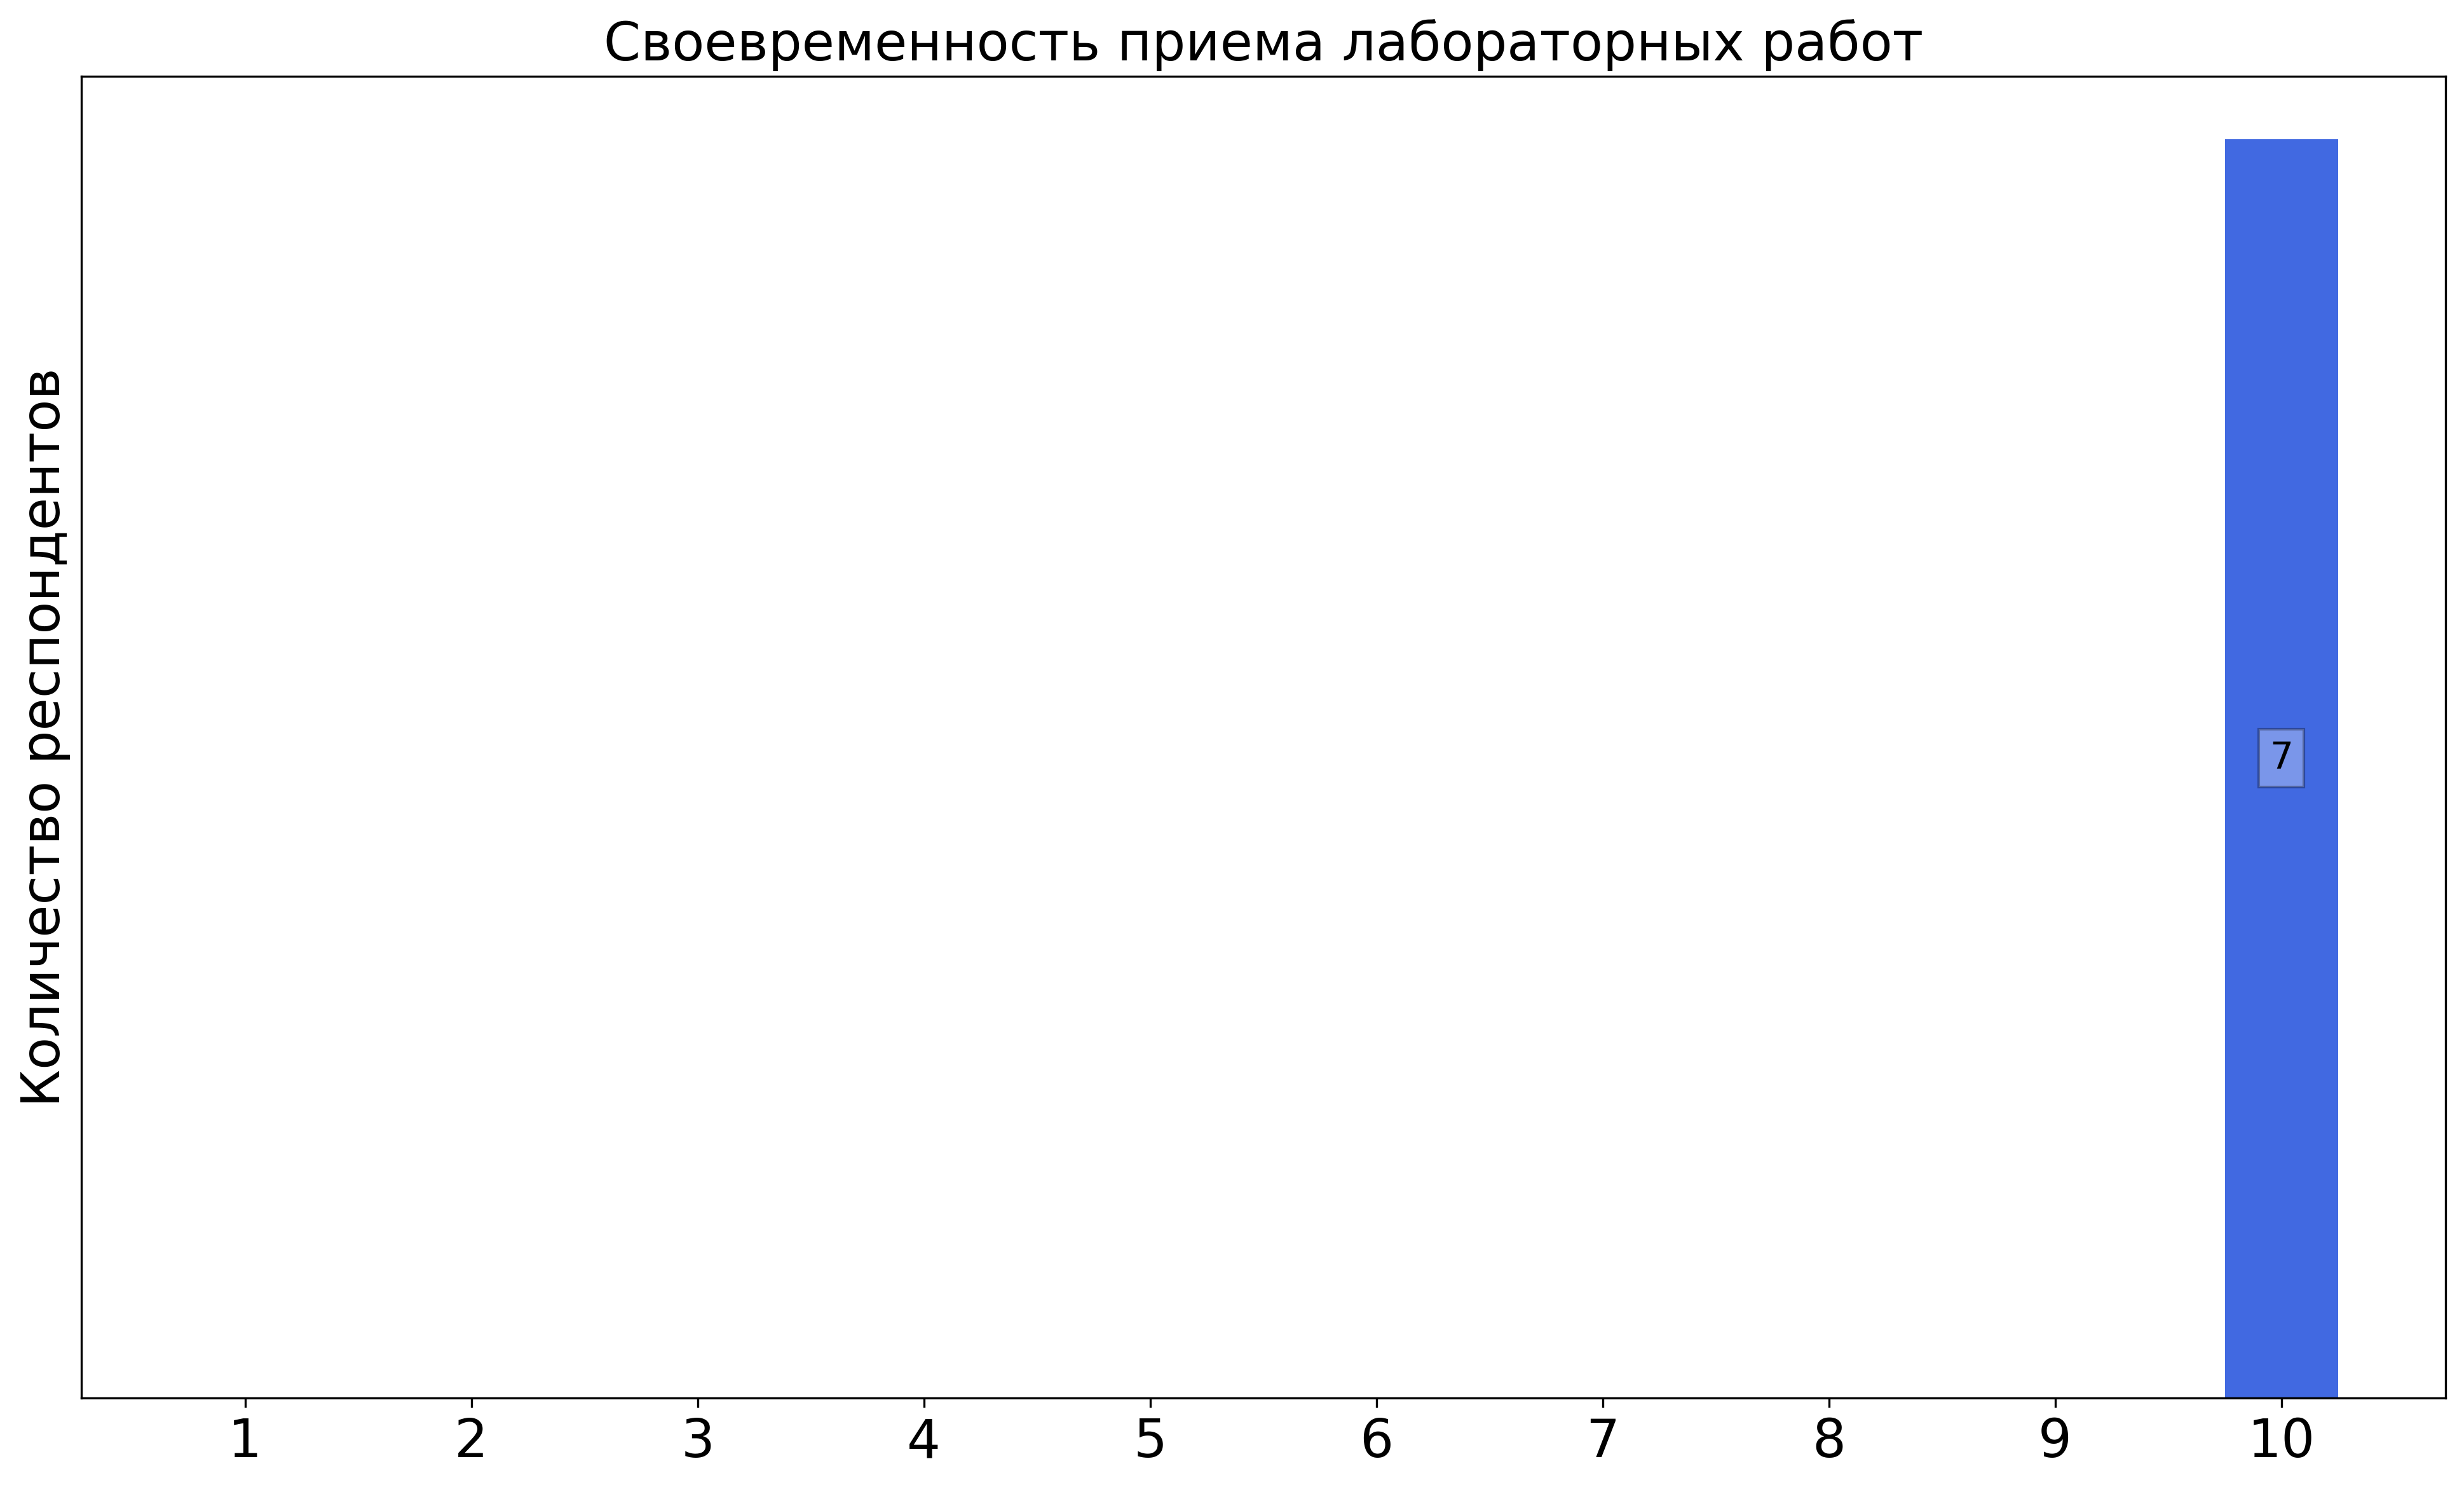
\includegraphics[width=\textwidth]{images/3 course/Аналоговая электроника/labniks-marks-Неешпапа А.В.-2.png}
			\end{subfigure}
			\begin{subfigure}[b]{0.45\textwidth}
				\centering
				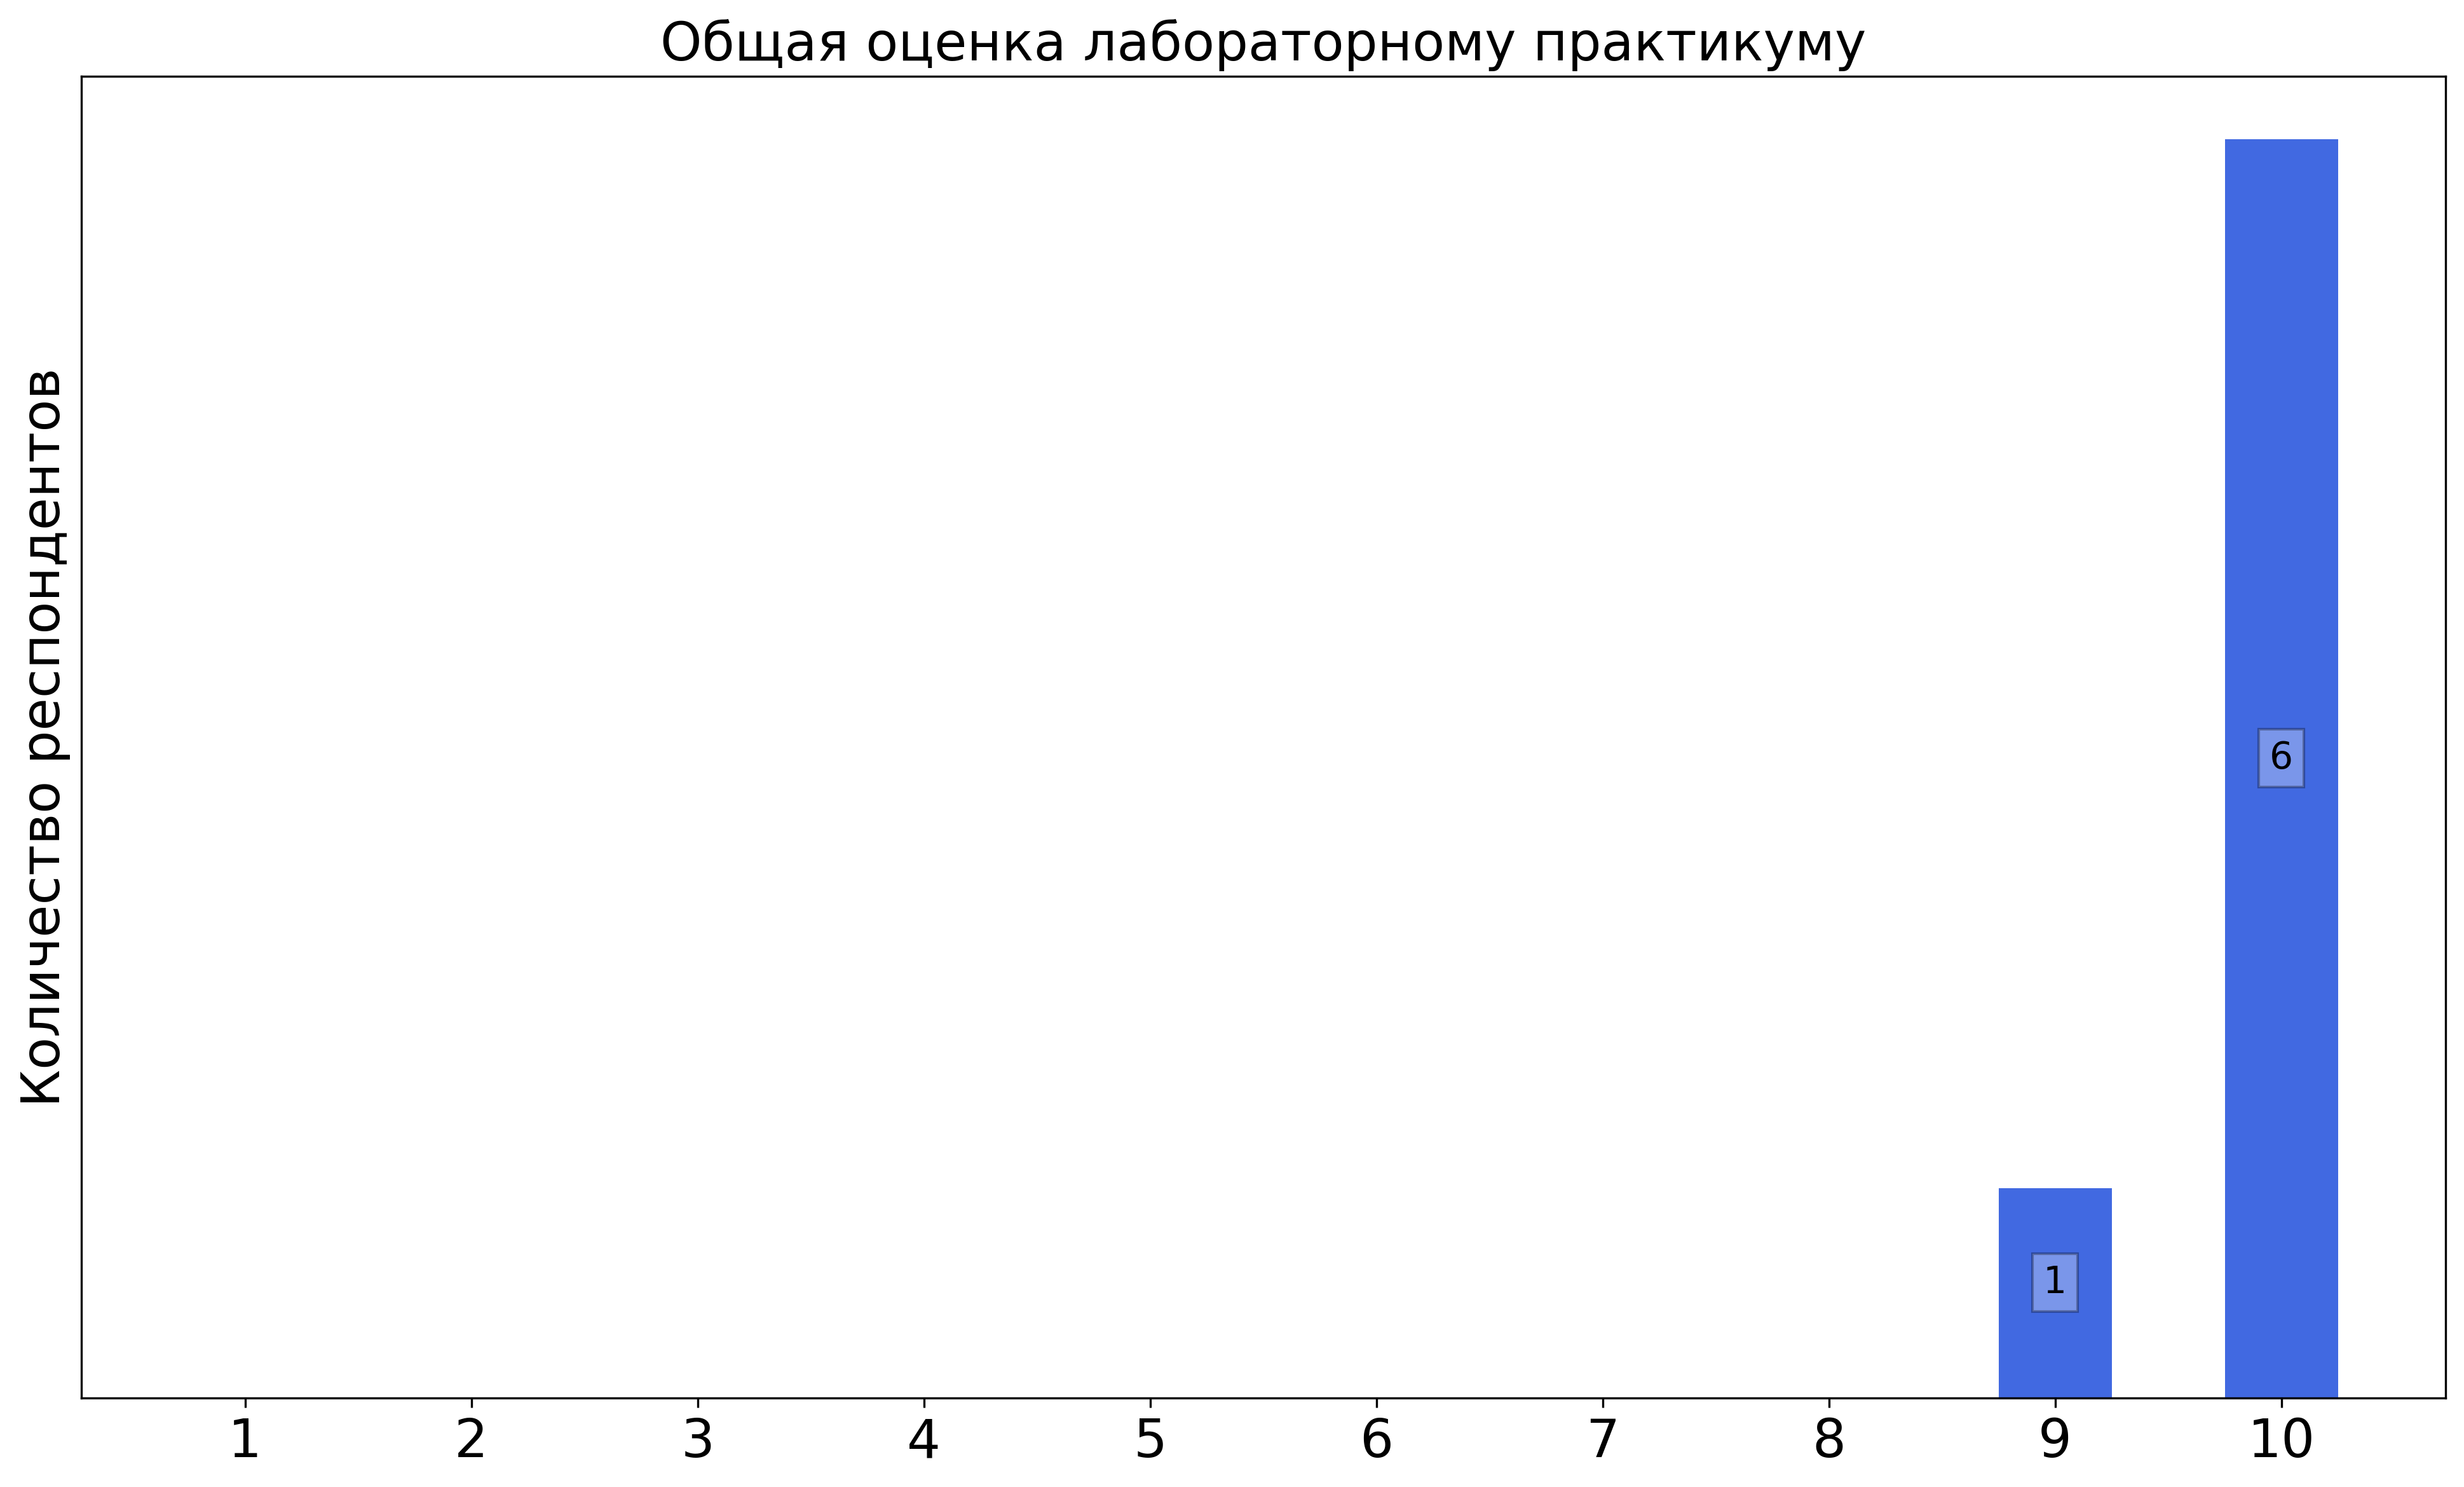
\includegraphics[width=\textwidth]{images/3 course/Аналоговая электроника/labniks-marks-Неешпапа А.В.-3.png}
			\end{subfigure}	
			\caption{Оценки респондентов о качестве преподавания лабораторных работ}
		\end{figure}

		\textbf{Комментарии студентов о преподавателе\protect\footnote{сохранены оригинальные орфография и пунктуация}}
            \begin{commentbox} 
                Преподаватель по лабораторным работам шикарно проводит занятия, доступно разъясняет материал. Благодаря Александру Владимировичу занятия были интересными и полезными 
            \end{commentbox} 
        
            \begin{commentbox} 
                Благодаря этому преподавателю мне понравились РТ лабы. Очень крутой мужик. Спасибо ему большое, прекрасно расшаривает, адекватно оценивает, можно просто поговорить по душам и всегда помогает на лабах. Приносил на ЛР тестеры для транзисторов и усилителей(это решала 90\% проблем) 
            \end{commentbox} 
        
            \begin{commentbox} 
                Главный кто вытягивал курс и даже почти заинтересовал уже почти мертвым в сердце предметом. Перед началом каждой лабы проводит большую теоретическую справку - понятно объясняет, отвечает на вопросы. Более того, есть ощущение, что он внедряет тебе некоторые инженерные концепции. После курса действительно есть ощущение, что я что-то из него вынес, запомнил и стал немного ближе к званию инженера 
            \end{commentbox} 
        
            \begin{commentbox} 
                Перед каждым занятием была небольшая лекция (минут на 40), на которой вводились основные формулы. В процессе выполнения показывал очень много различных моментов, которые могли бы помешать выполнению лаб 
            \end{commentbox} 
        
            \begin{commentbox} 
                Хороший в меру строгий преподаватель, помогает на выполнении, рассказывает теорию, помогает зашарить 
            \end{commentbox} 
        
            \begin{commentbox} 
                Нужно осовременивать. Сейчас курс кажется устаревшим, а немногочисленные полученные знания неактуальными.  
            \end{commentbox}


    \subsubsection{Отзыв студентов о лабораторных работах. Преподаватель: Русскин С.О.}
		\begin{figure}[H]
			\centering
			\begin{subfigure}[b]{0.45\textwidth}
				\centering
				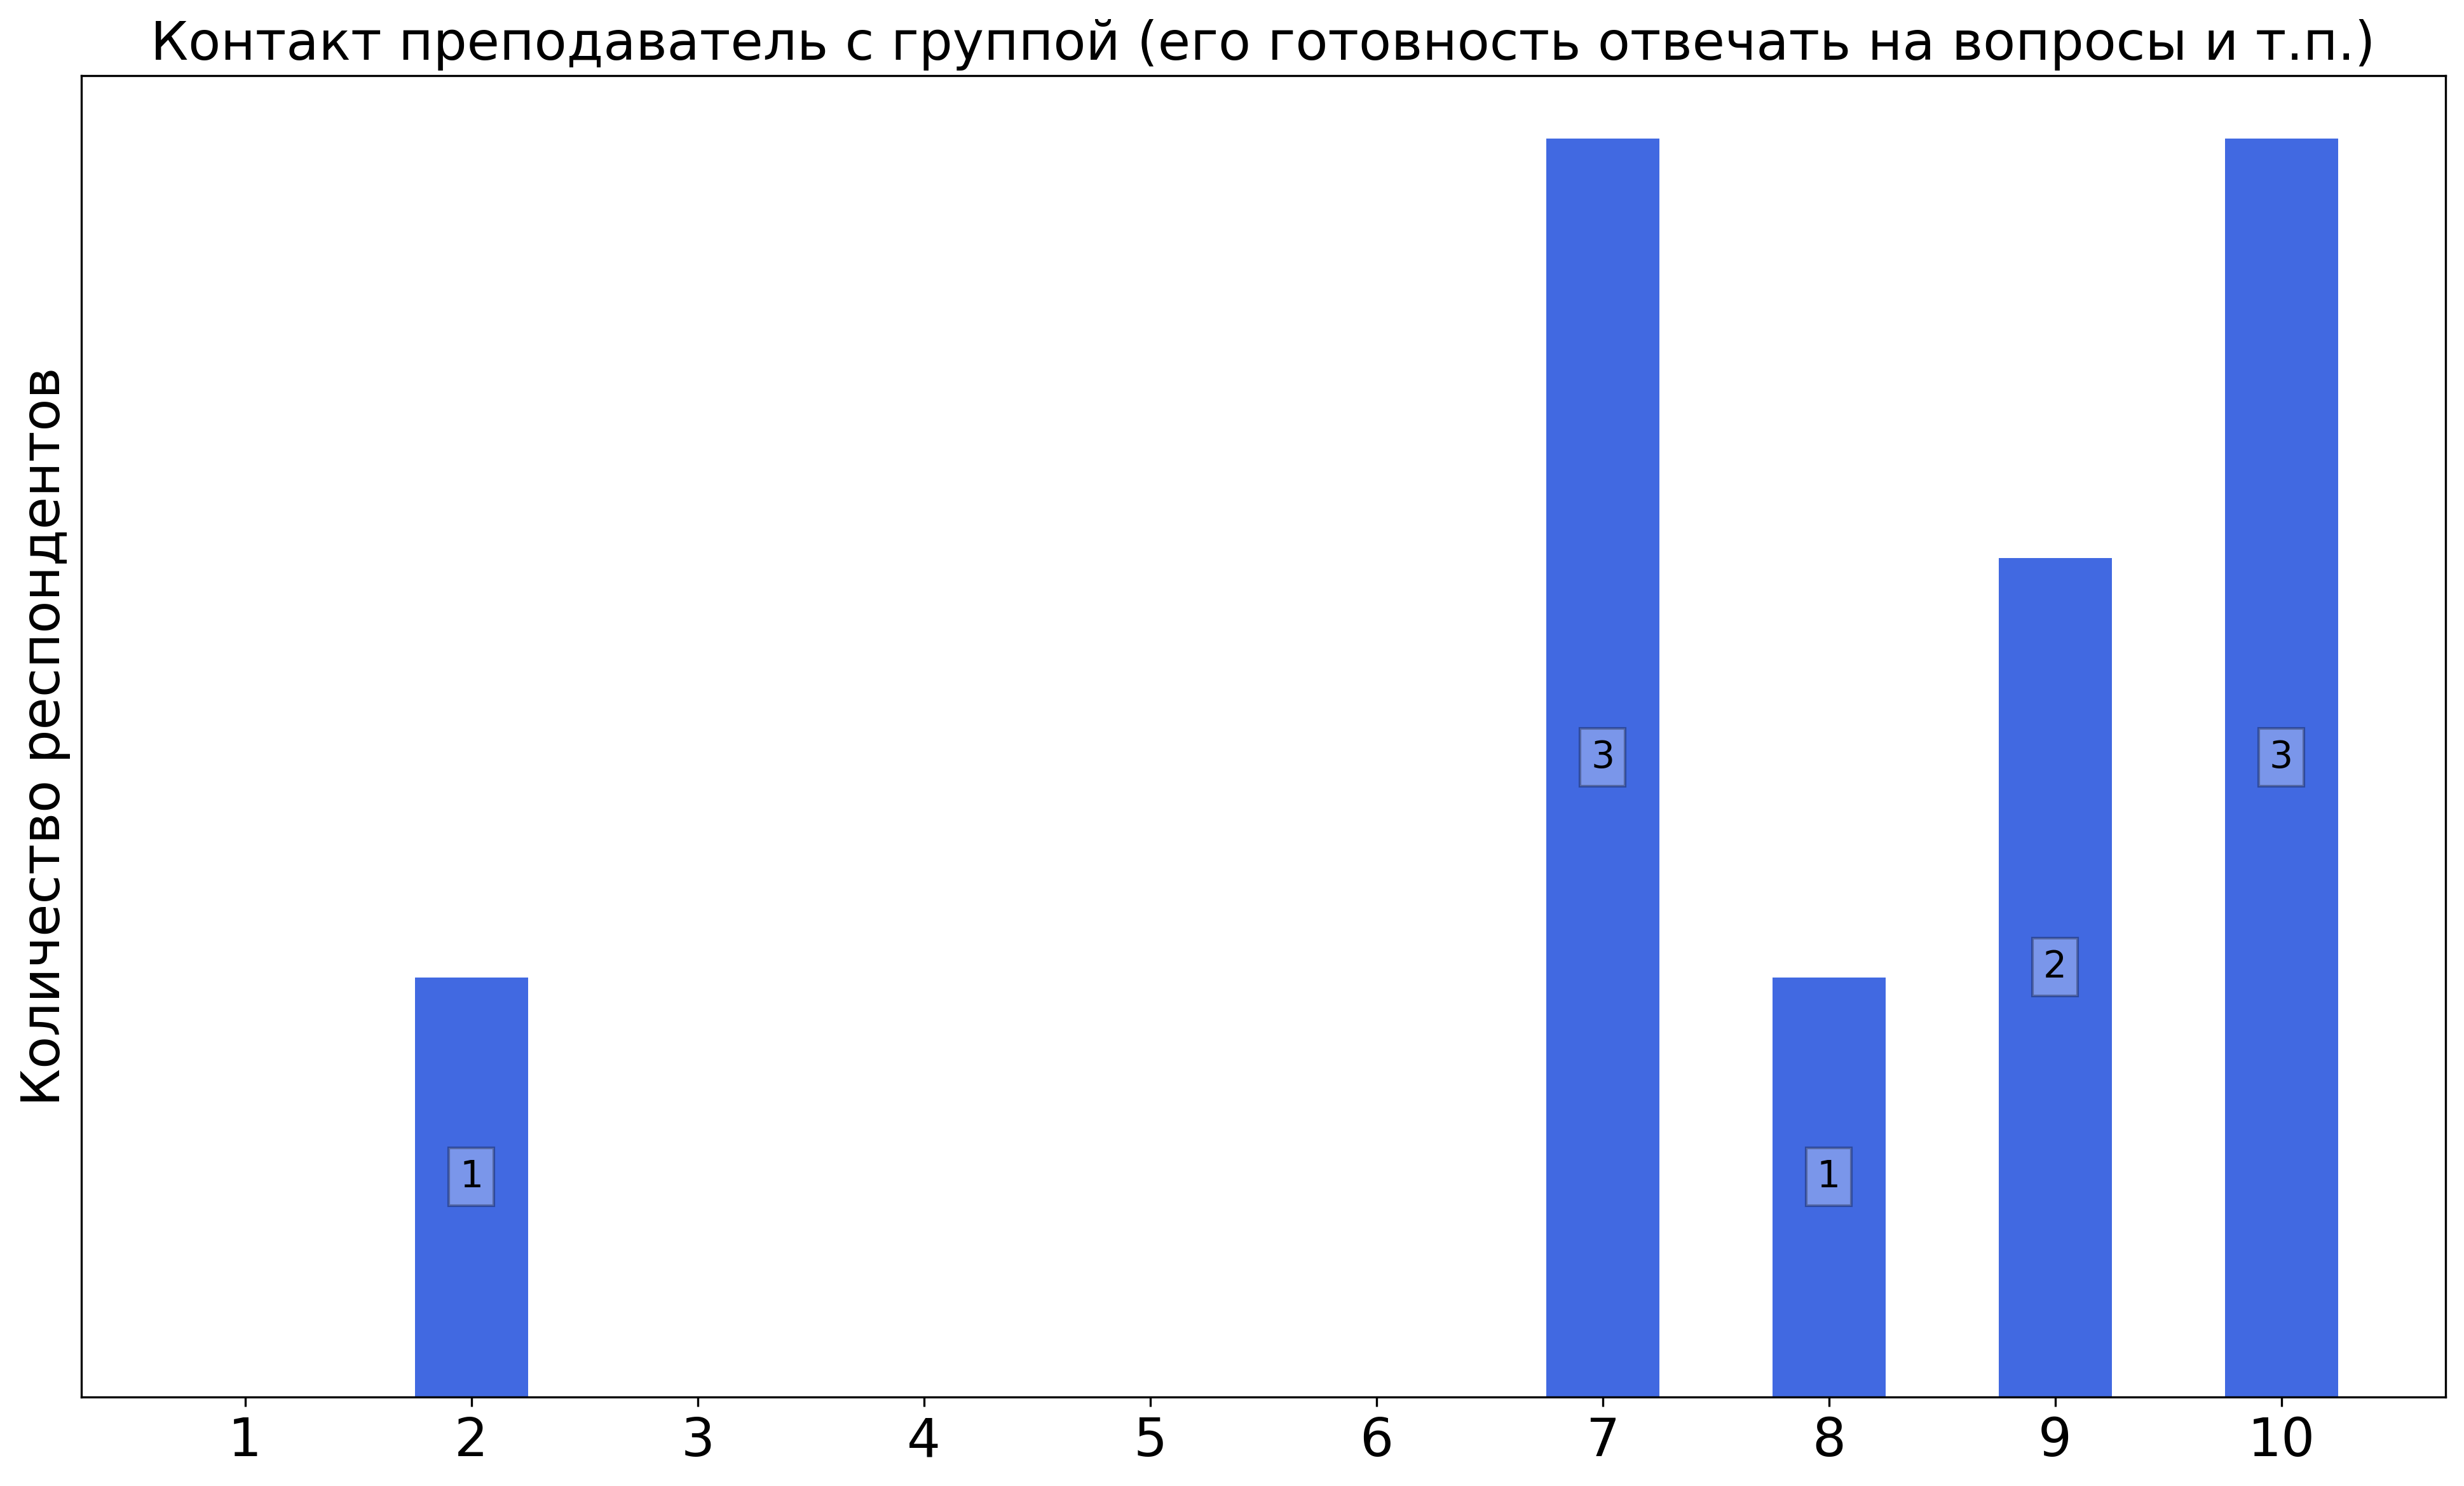
\includegraphics[width=\textwidth]{images/3 course/Аналоговая электроника/labniks-marks-Русскин С.О.-0.png}
			\end{subfigure}
			\begin{subfigure}[b]{0.45\textwidth}
				\centering
				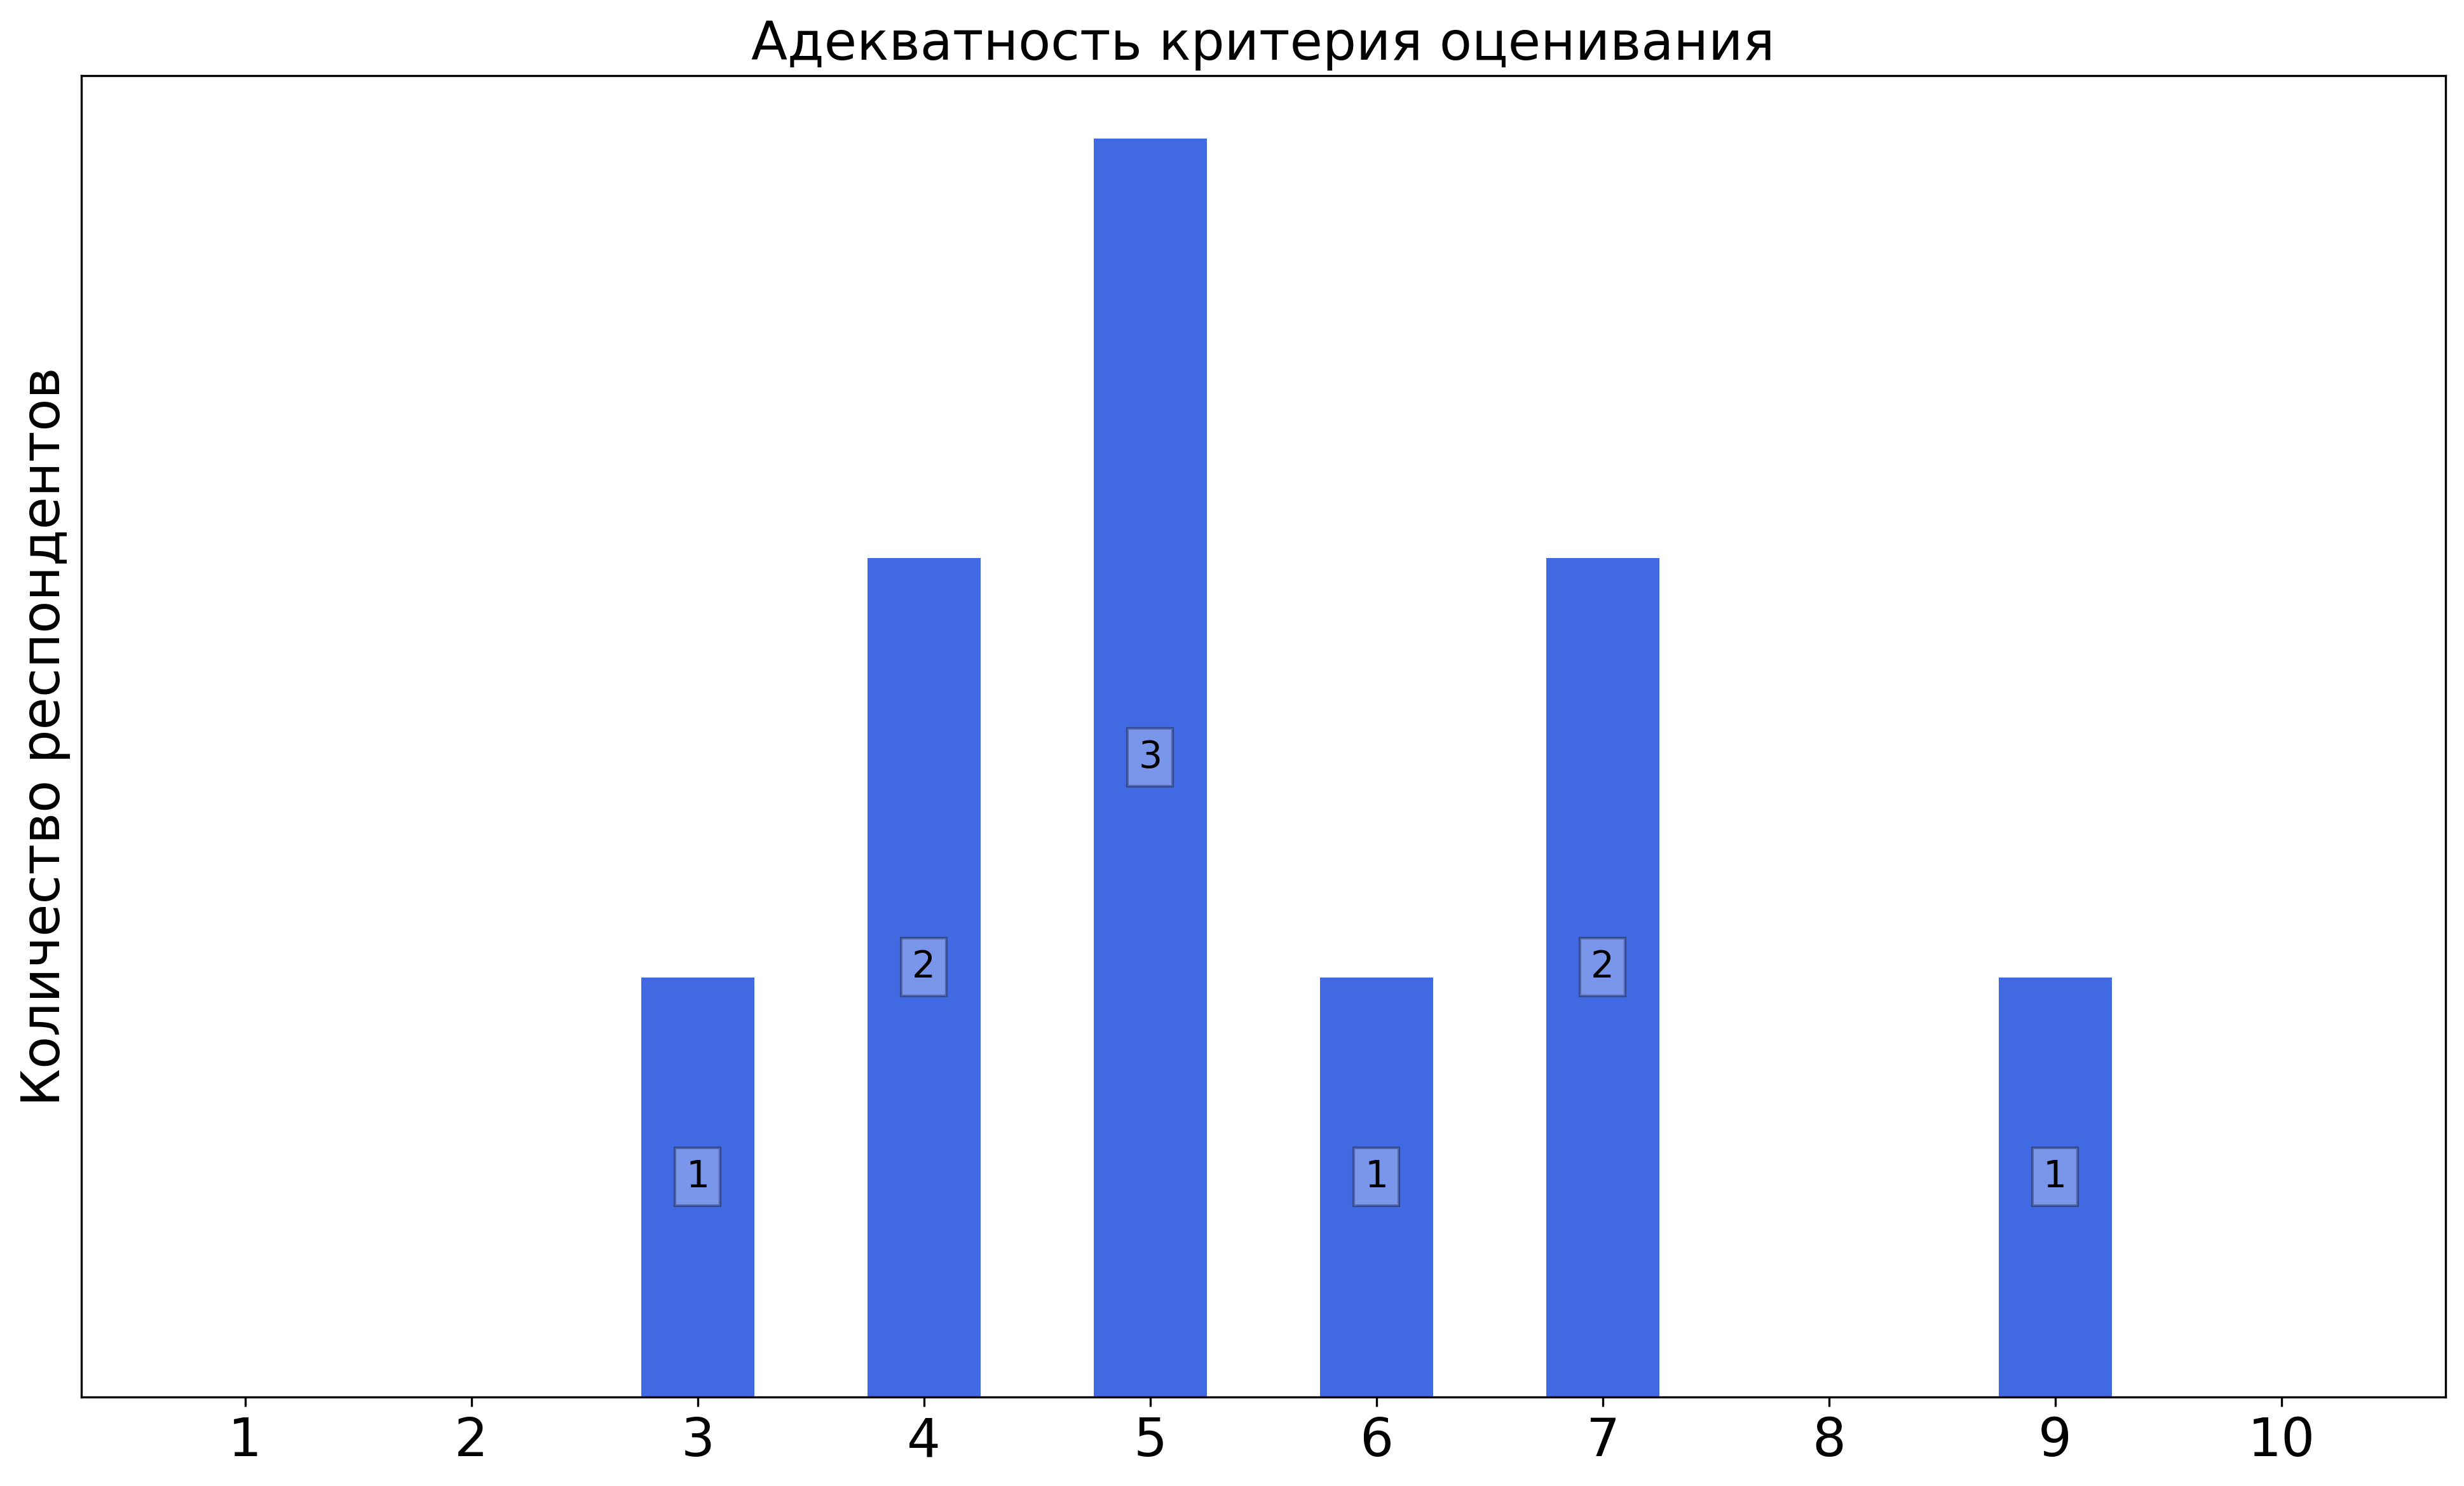
\includegraphics[width=\textwidth]{images/3 course/Аналоговая электроника/labniks-marks-Русскин С.О.-1.png}
			\end{subfigure}
			\begin{subfigure}[b]{0.45\textwidth}
				\centering
				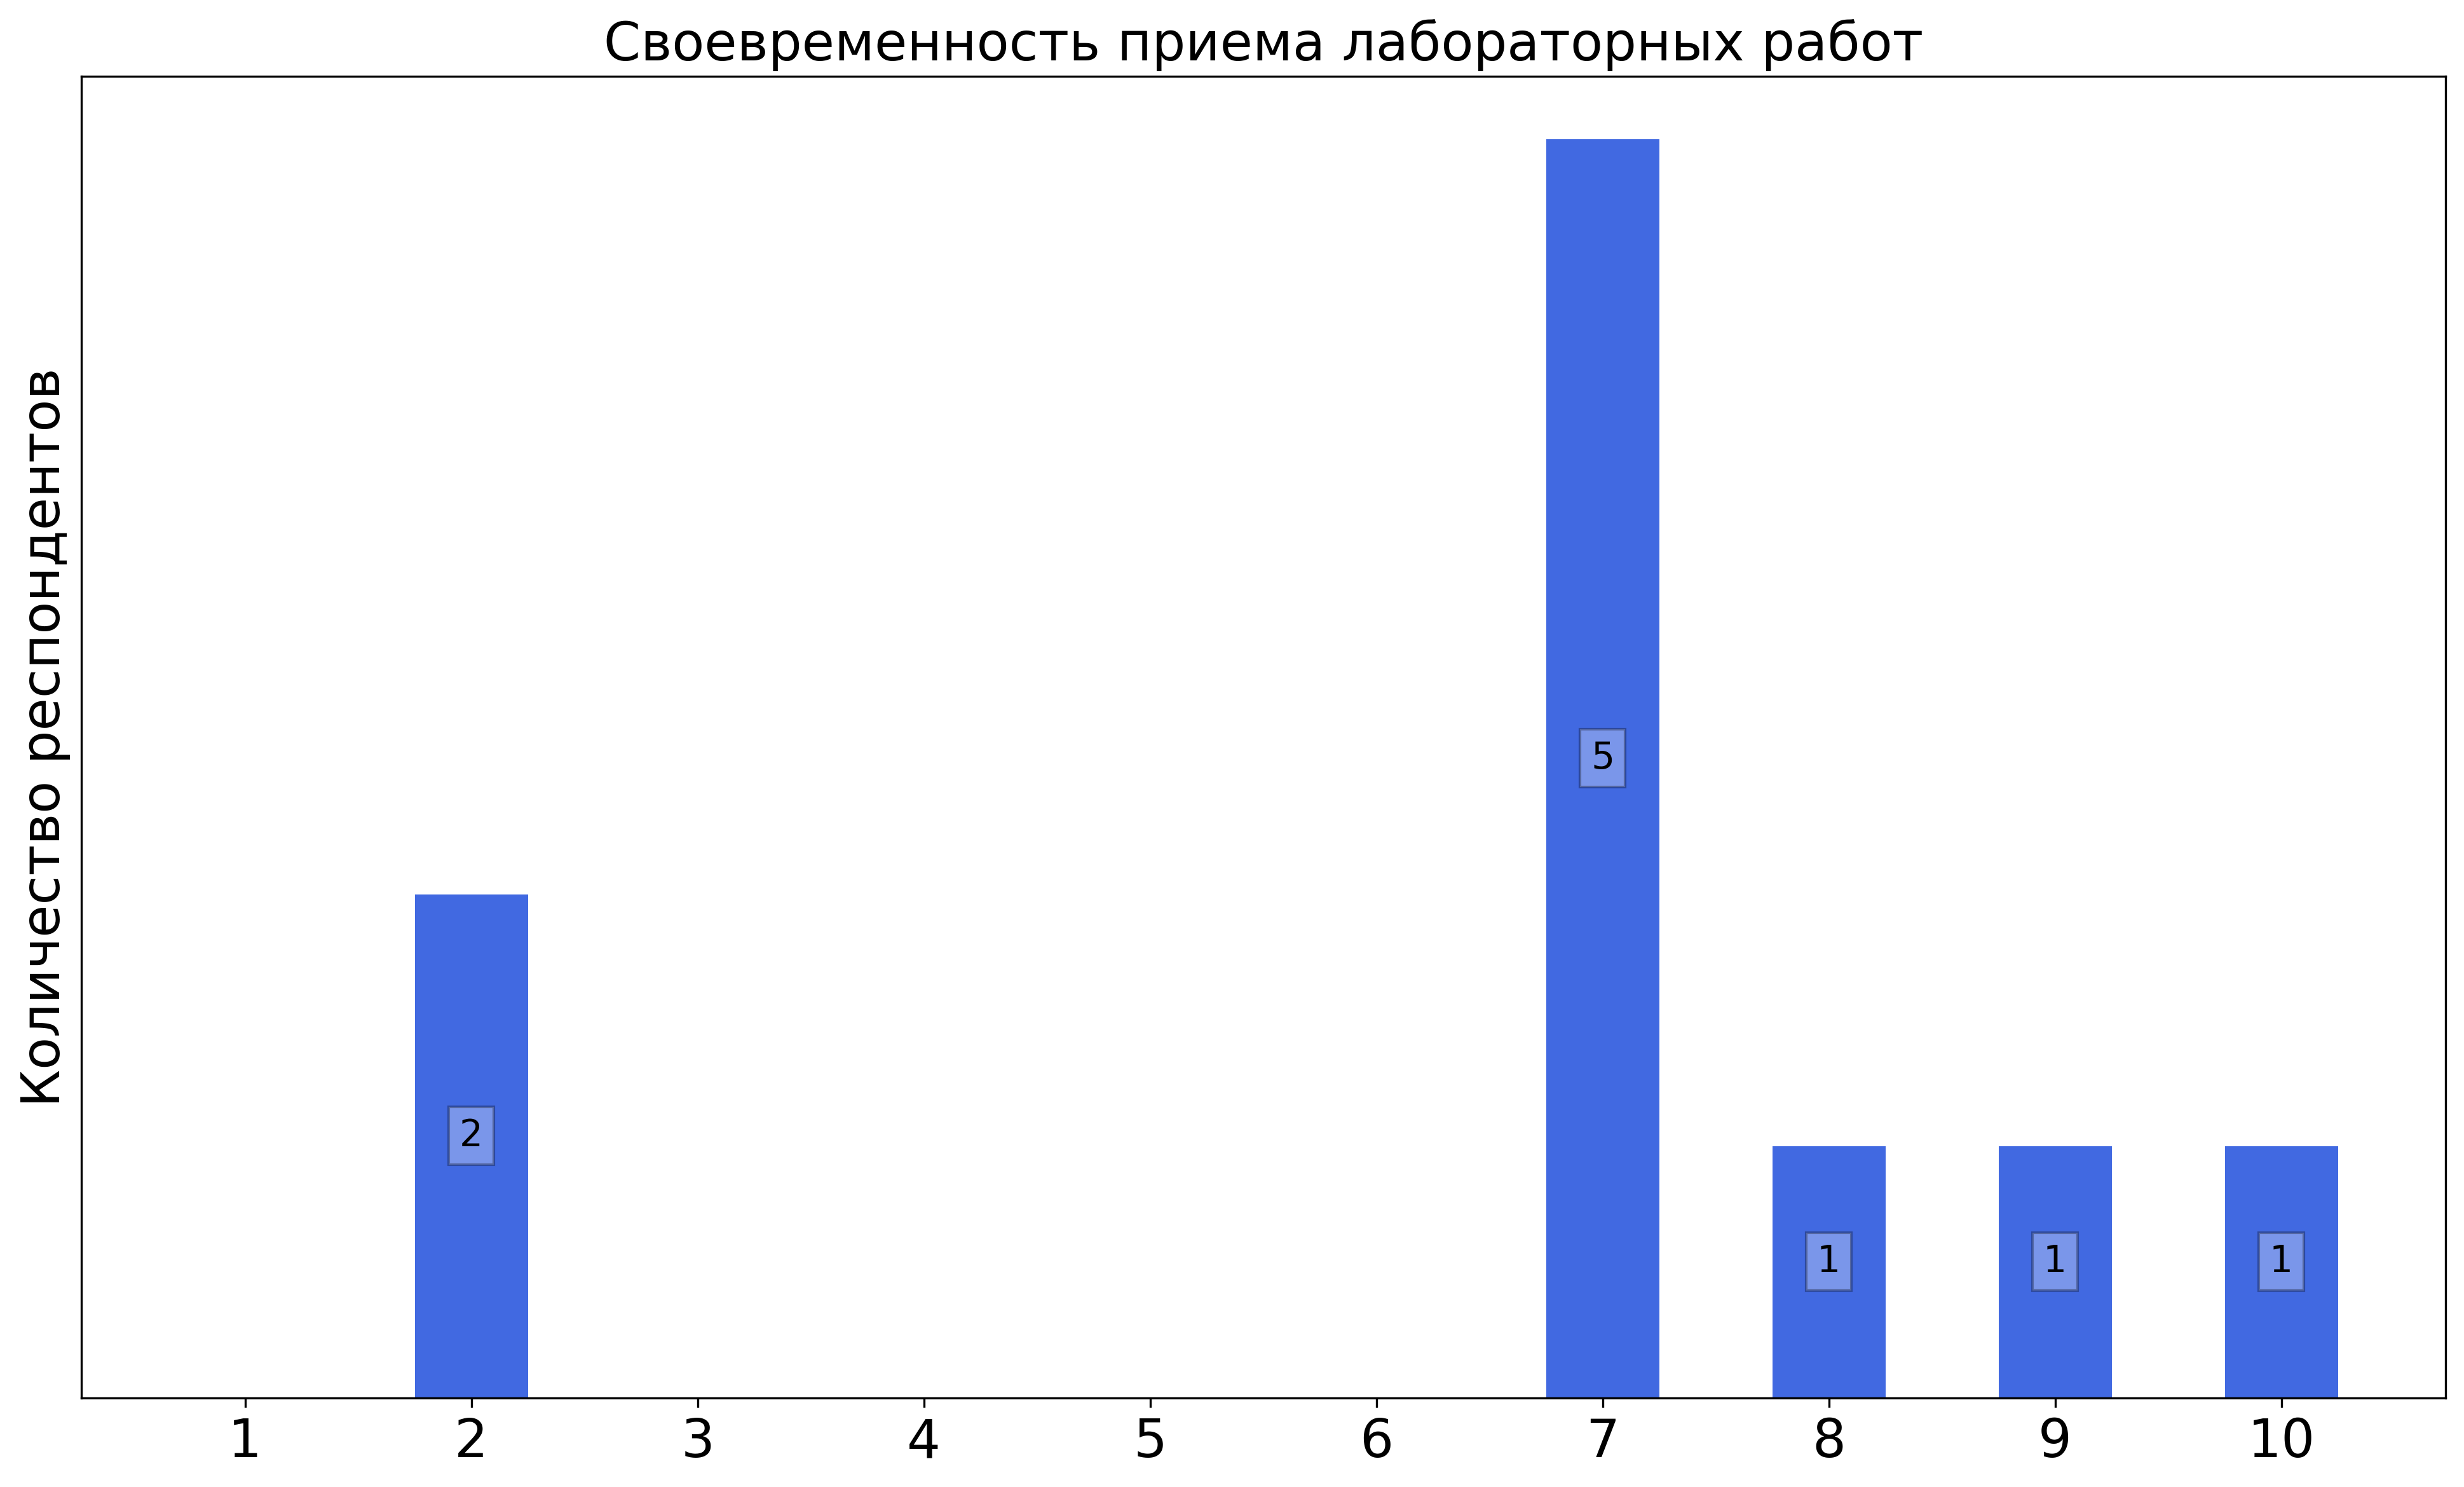
\includegraphics[width=\textwidth]{images/3 course/Аналоговая электроника/labniks-marks-Русскин С.О.-2.png}
			\end{subfigure}
			\begin{subfigure}[b]{0.45\textwidth}
				\centering
				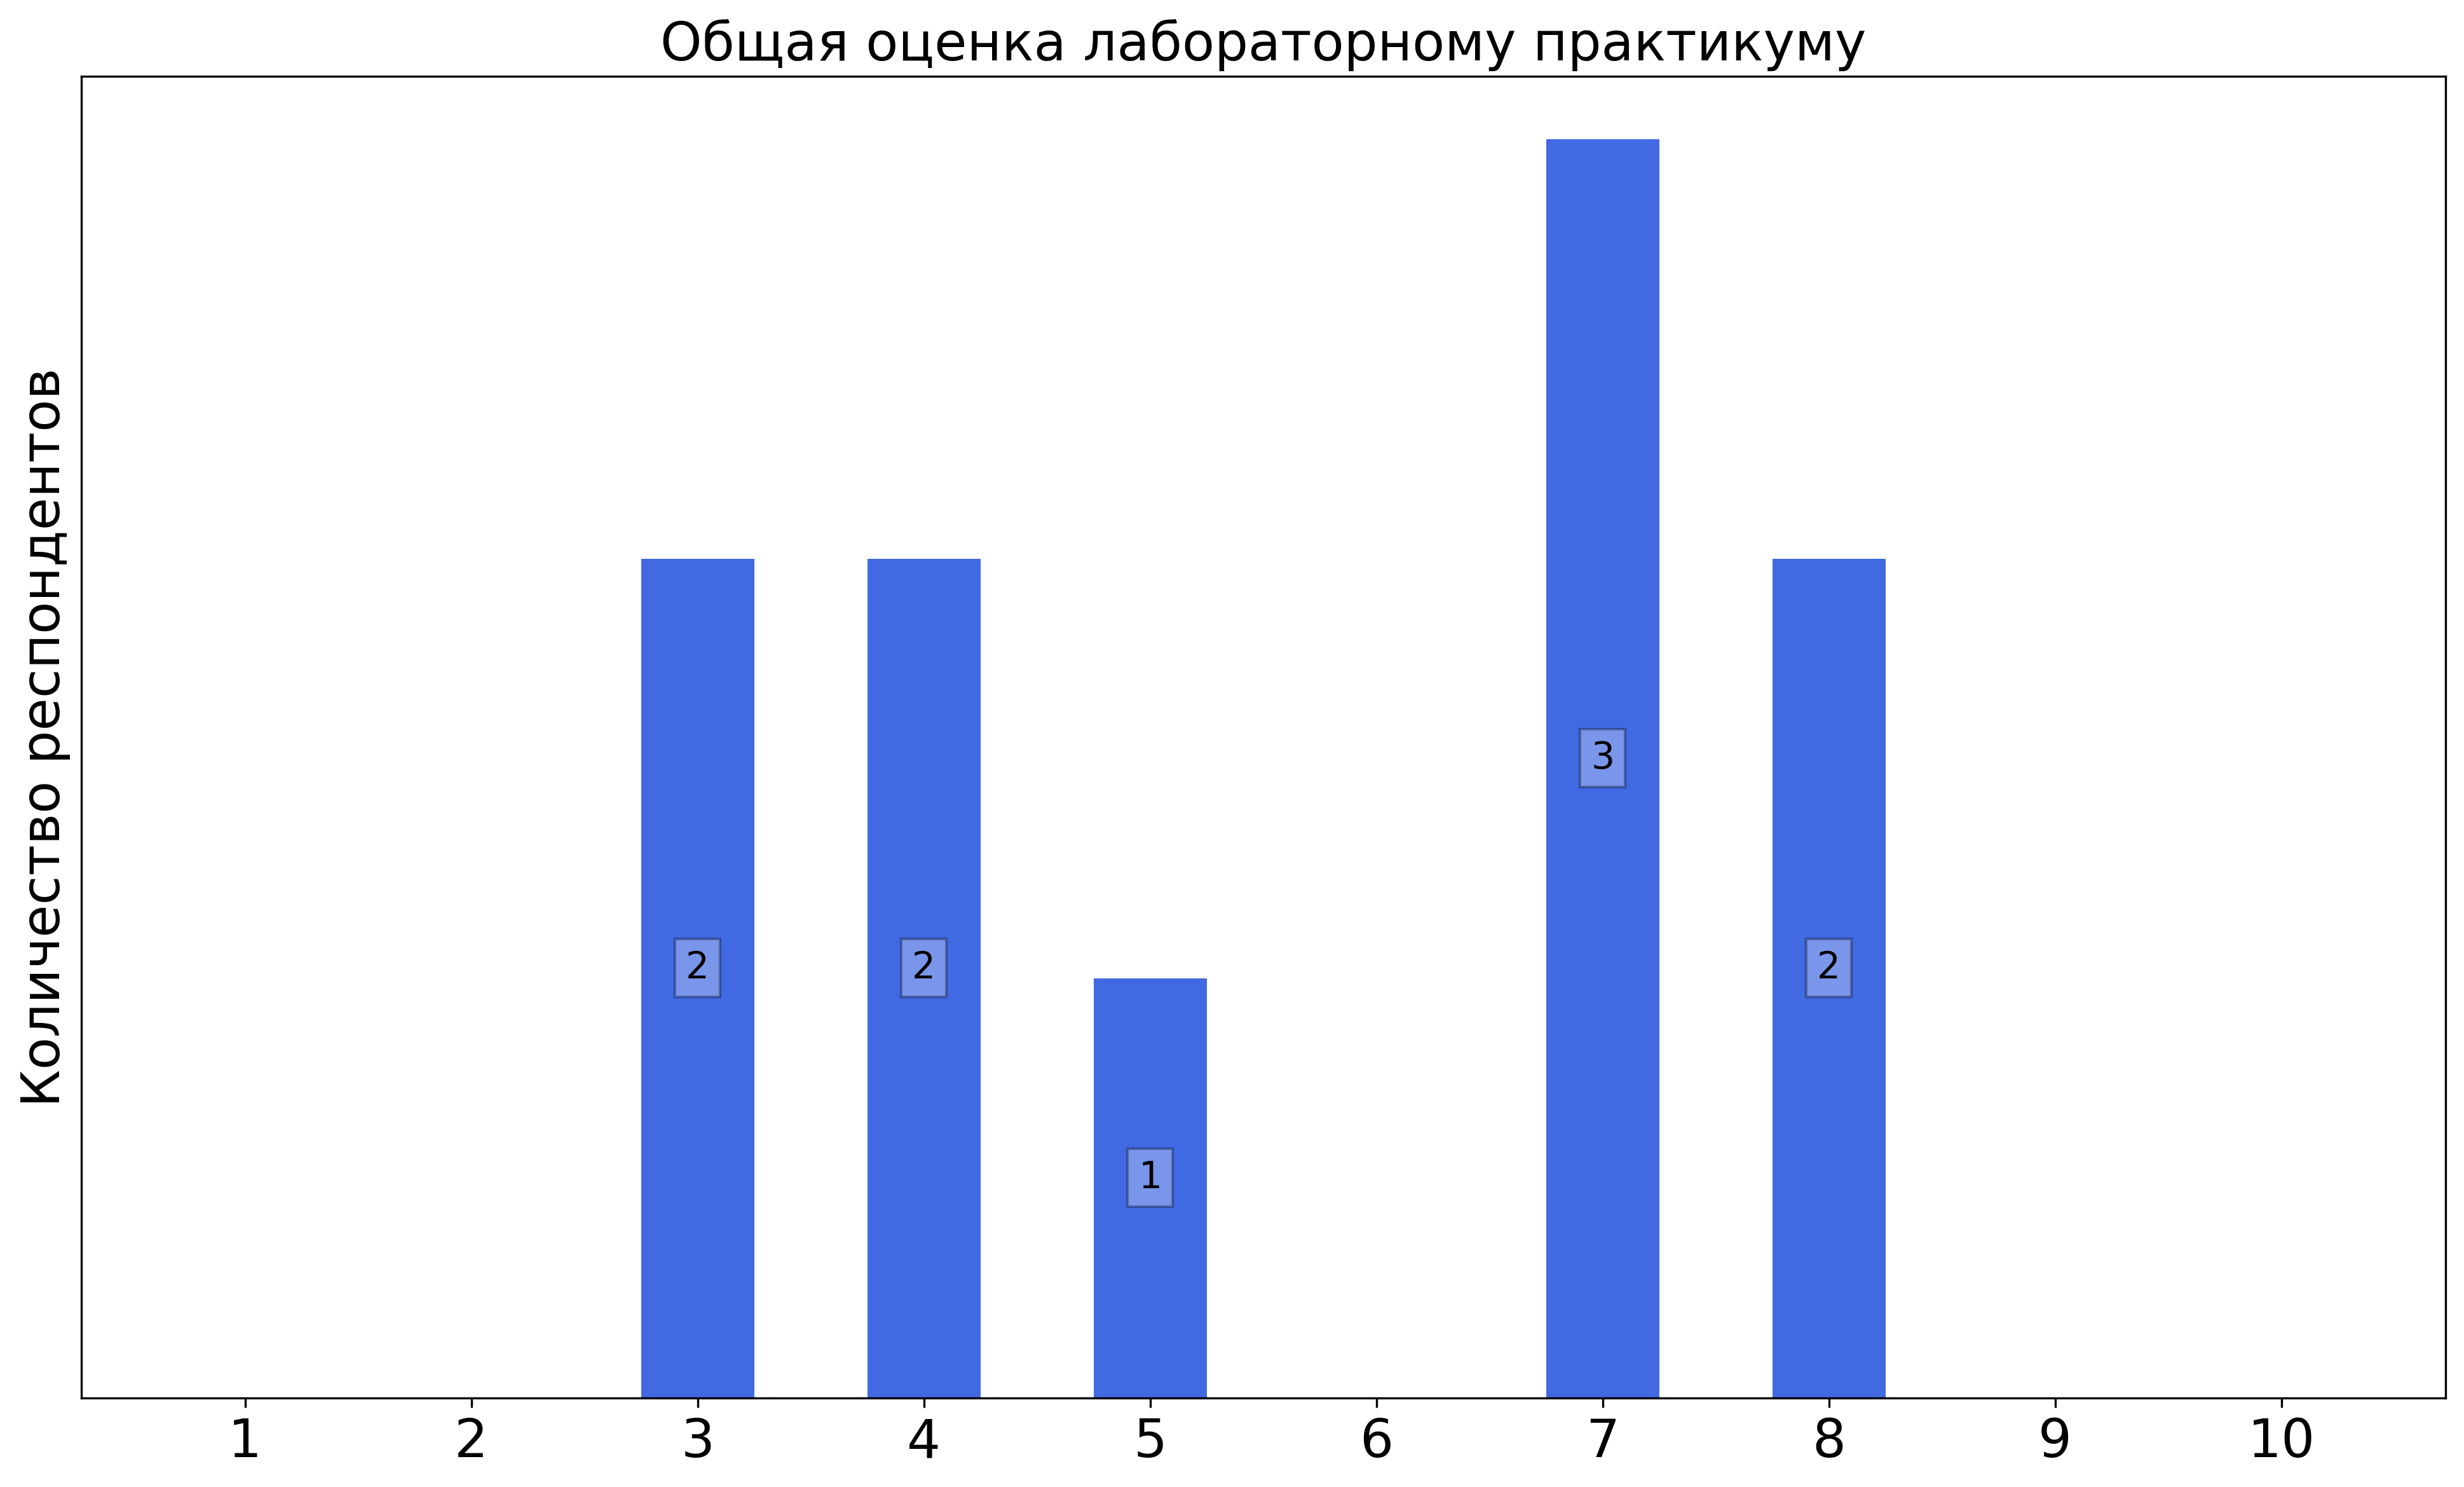
\includegraphics[width=\textwidth]{images/3 course/Аналоговая электроника/labniks-marks-Русскин С.О.-3.png}
			\end{subfigure}	
			\caption{Оценки респондентов о качестве преподавания лабораторных работ}
		\end{figure}

		\textbf{Комментарии студентов о преподавателе\protect\footnote{сохранены оригинальные орфография и пунктуация}}
            \begin{commentbox} 
                Не особо понятные методички 
            \end{commentbox} 

            \begin{commentbox} 
                Сложность в понимании материала изложеного в методичках.  
            \end{commentbox} 

            \begin{commentbox} 
                Преподаватель лучше, чем большинство на кафедре, тем не менее, кажется, что из курса даже после экзамена я не вынес ничего. Сдача лабораторных работ проходит в виде просмотра отчета и вопросов по нему, после чего идешь разбираться и искать ответ в методичке или книжке Ларина - обычно зацепляясь за знакомые буквы. Сдачи долгие, иногда по 4 часа 
            \end{commentbox} 

            \begin{commentbox} 
                Преподаватель как будто абсолютно ни в чем не заинтересован, теория почти никак не поясняется. Сдача происходит дольше выделенного времени, часто приходилось оставаться и на +1.5 часа сверху, оценки выставляются не понятно по какому принципу. Лабораторные ужасные. 
            \end{commentbox}


    \subsubsection{Отзыв студентов о лабораторных работах. Преподаватель: Тужилкин В.А.}
		\begin{figure}[H]
			\centering
			\begin{subfigure}[b]{0.45\textwidth}
				\centering
				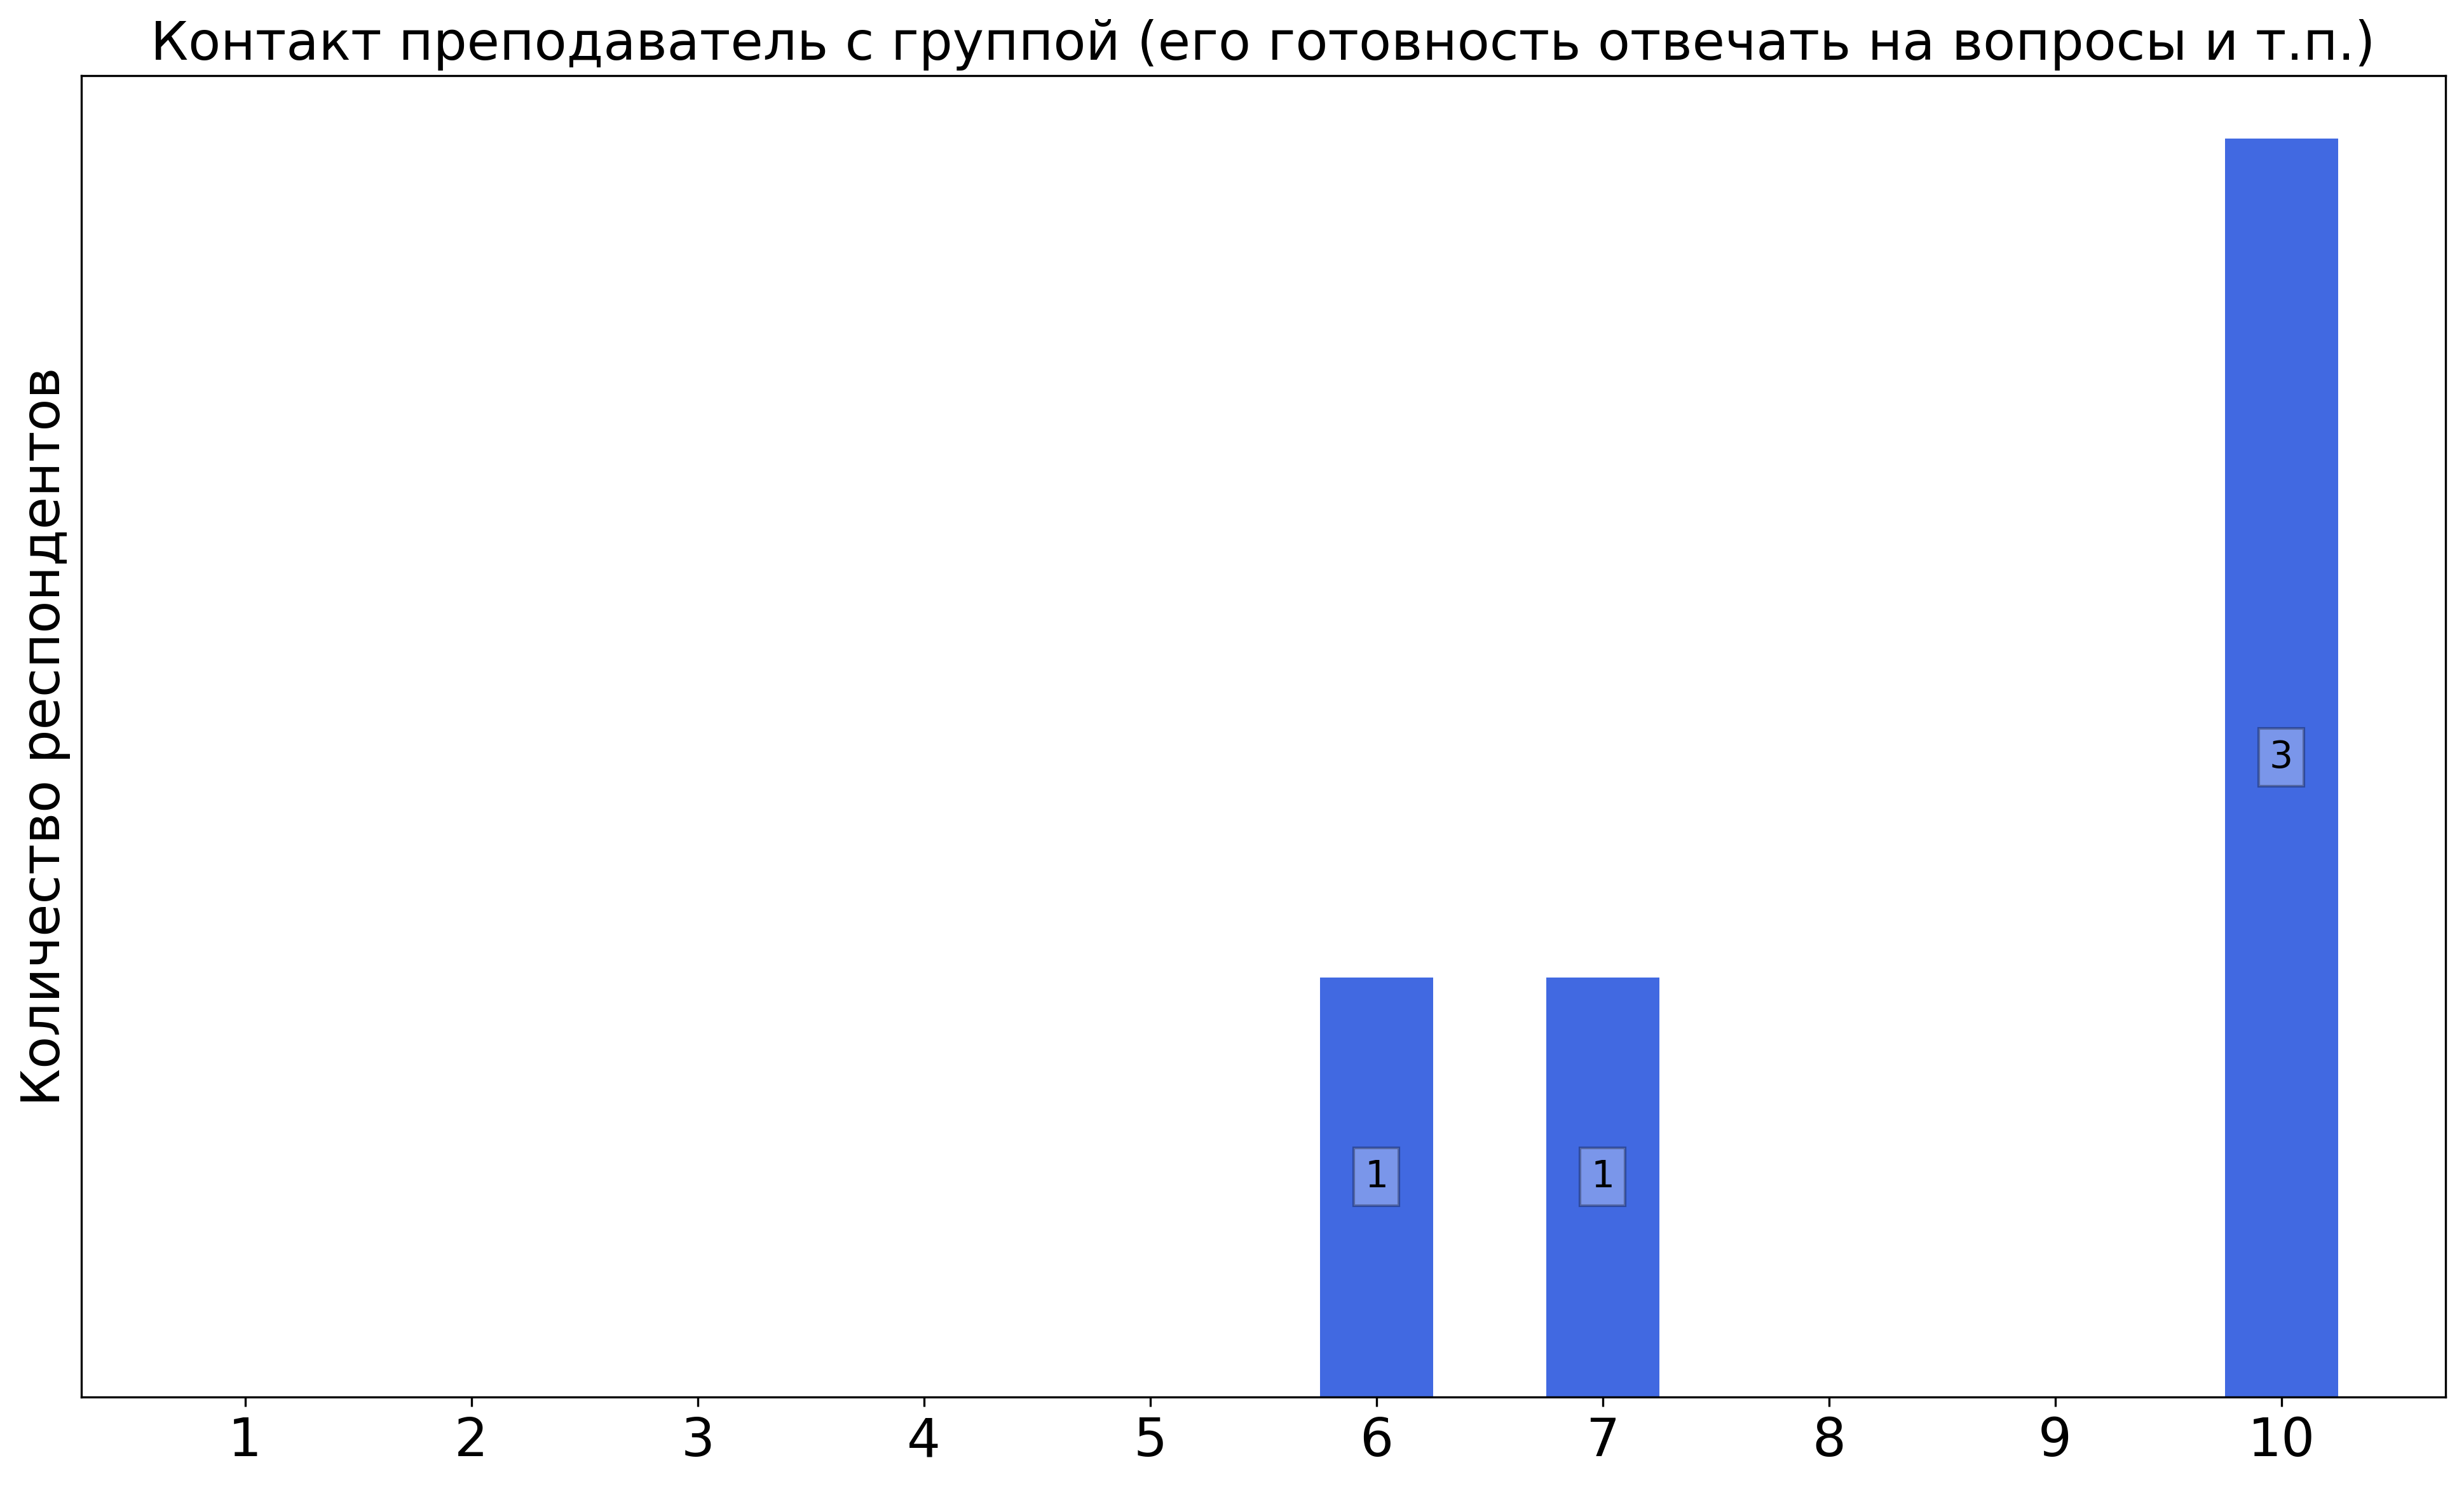
\includegraphics[width=\textwidth]{images/3 course/Аналоговая электроника/labniks-marks-Тужилкин В.А.-0.png}
			\end{subfigure}
			\begin{subfigure}[b]{0.45\textwidth}
				\centering
				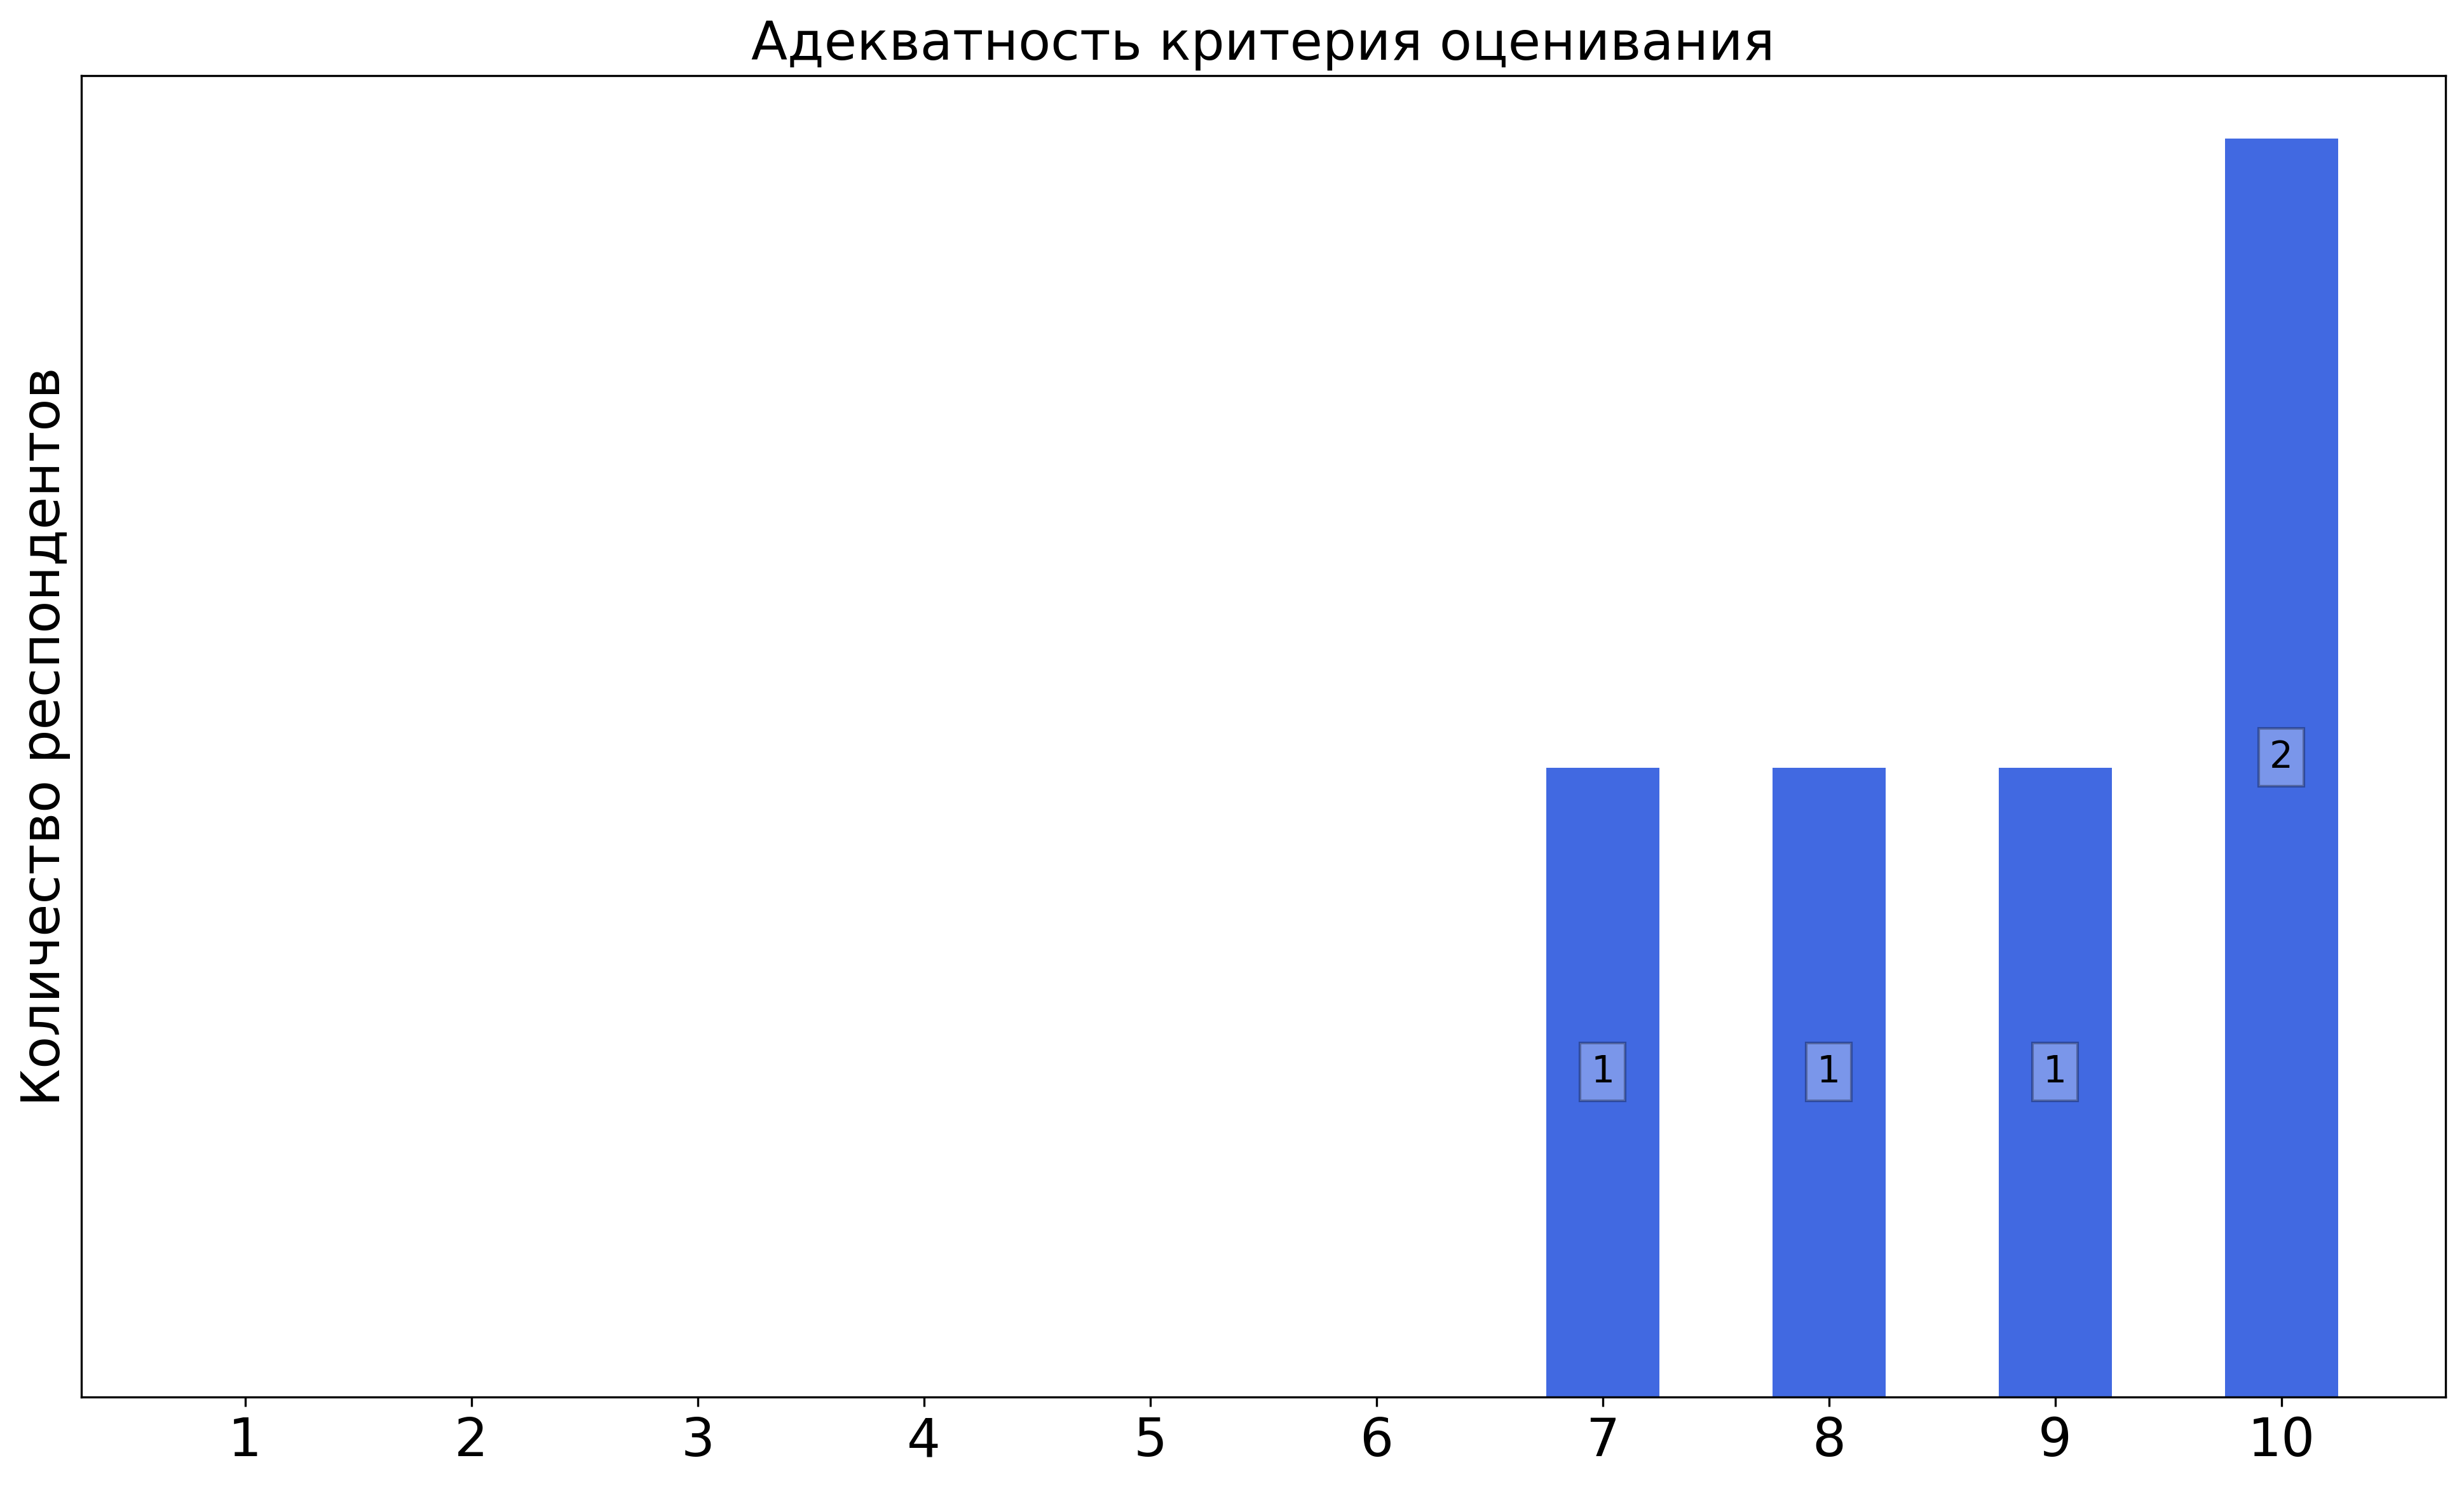
\includegraphics[width=\textwidth]{images/3 course/Аналоговая электроника/labniks-marks-Тужилкин В.А.-1.png}
			\end{subfigure}
			\begin{subfigure}[b]{0.45\textwidth}
				\centering
				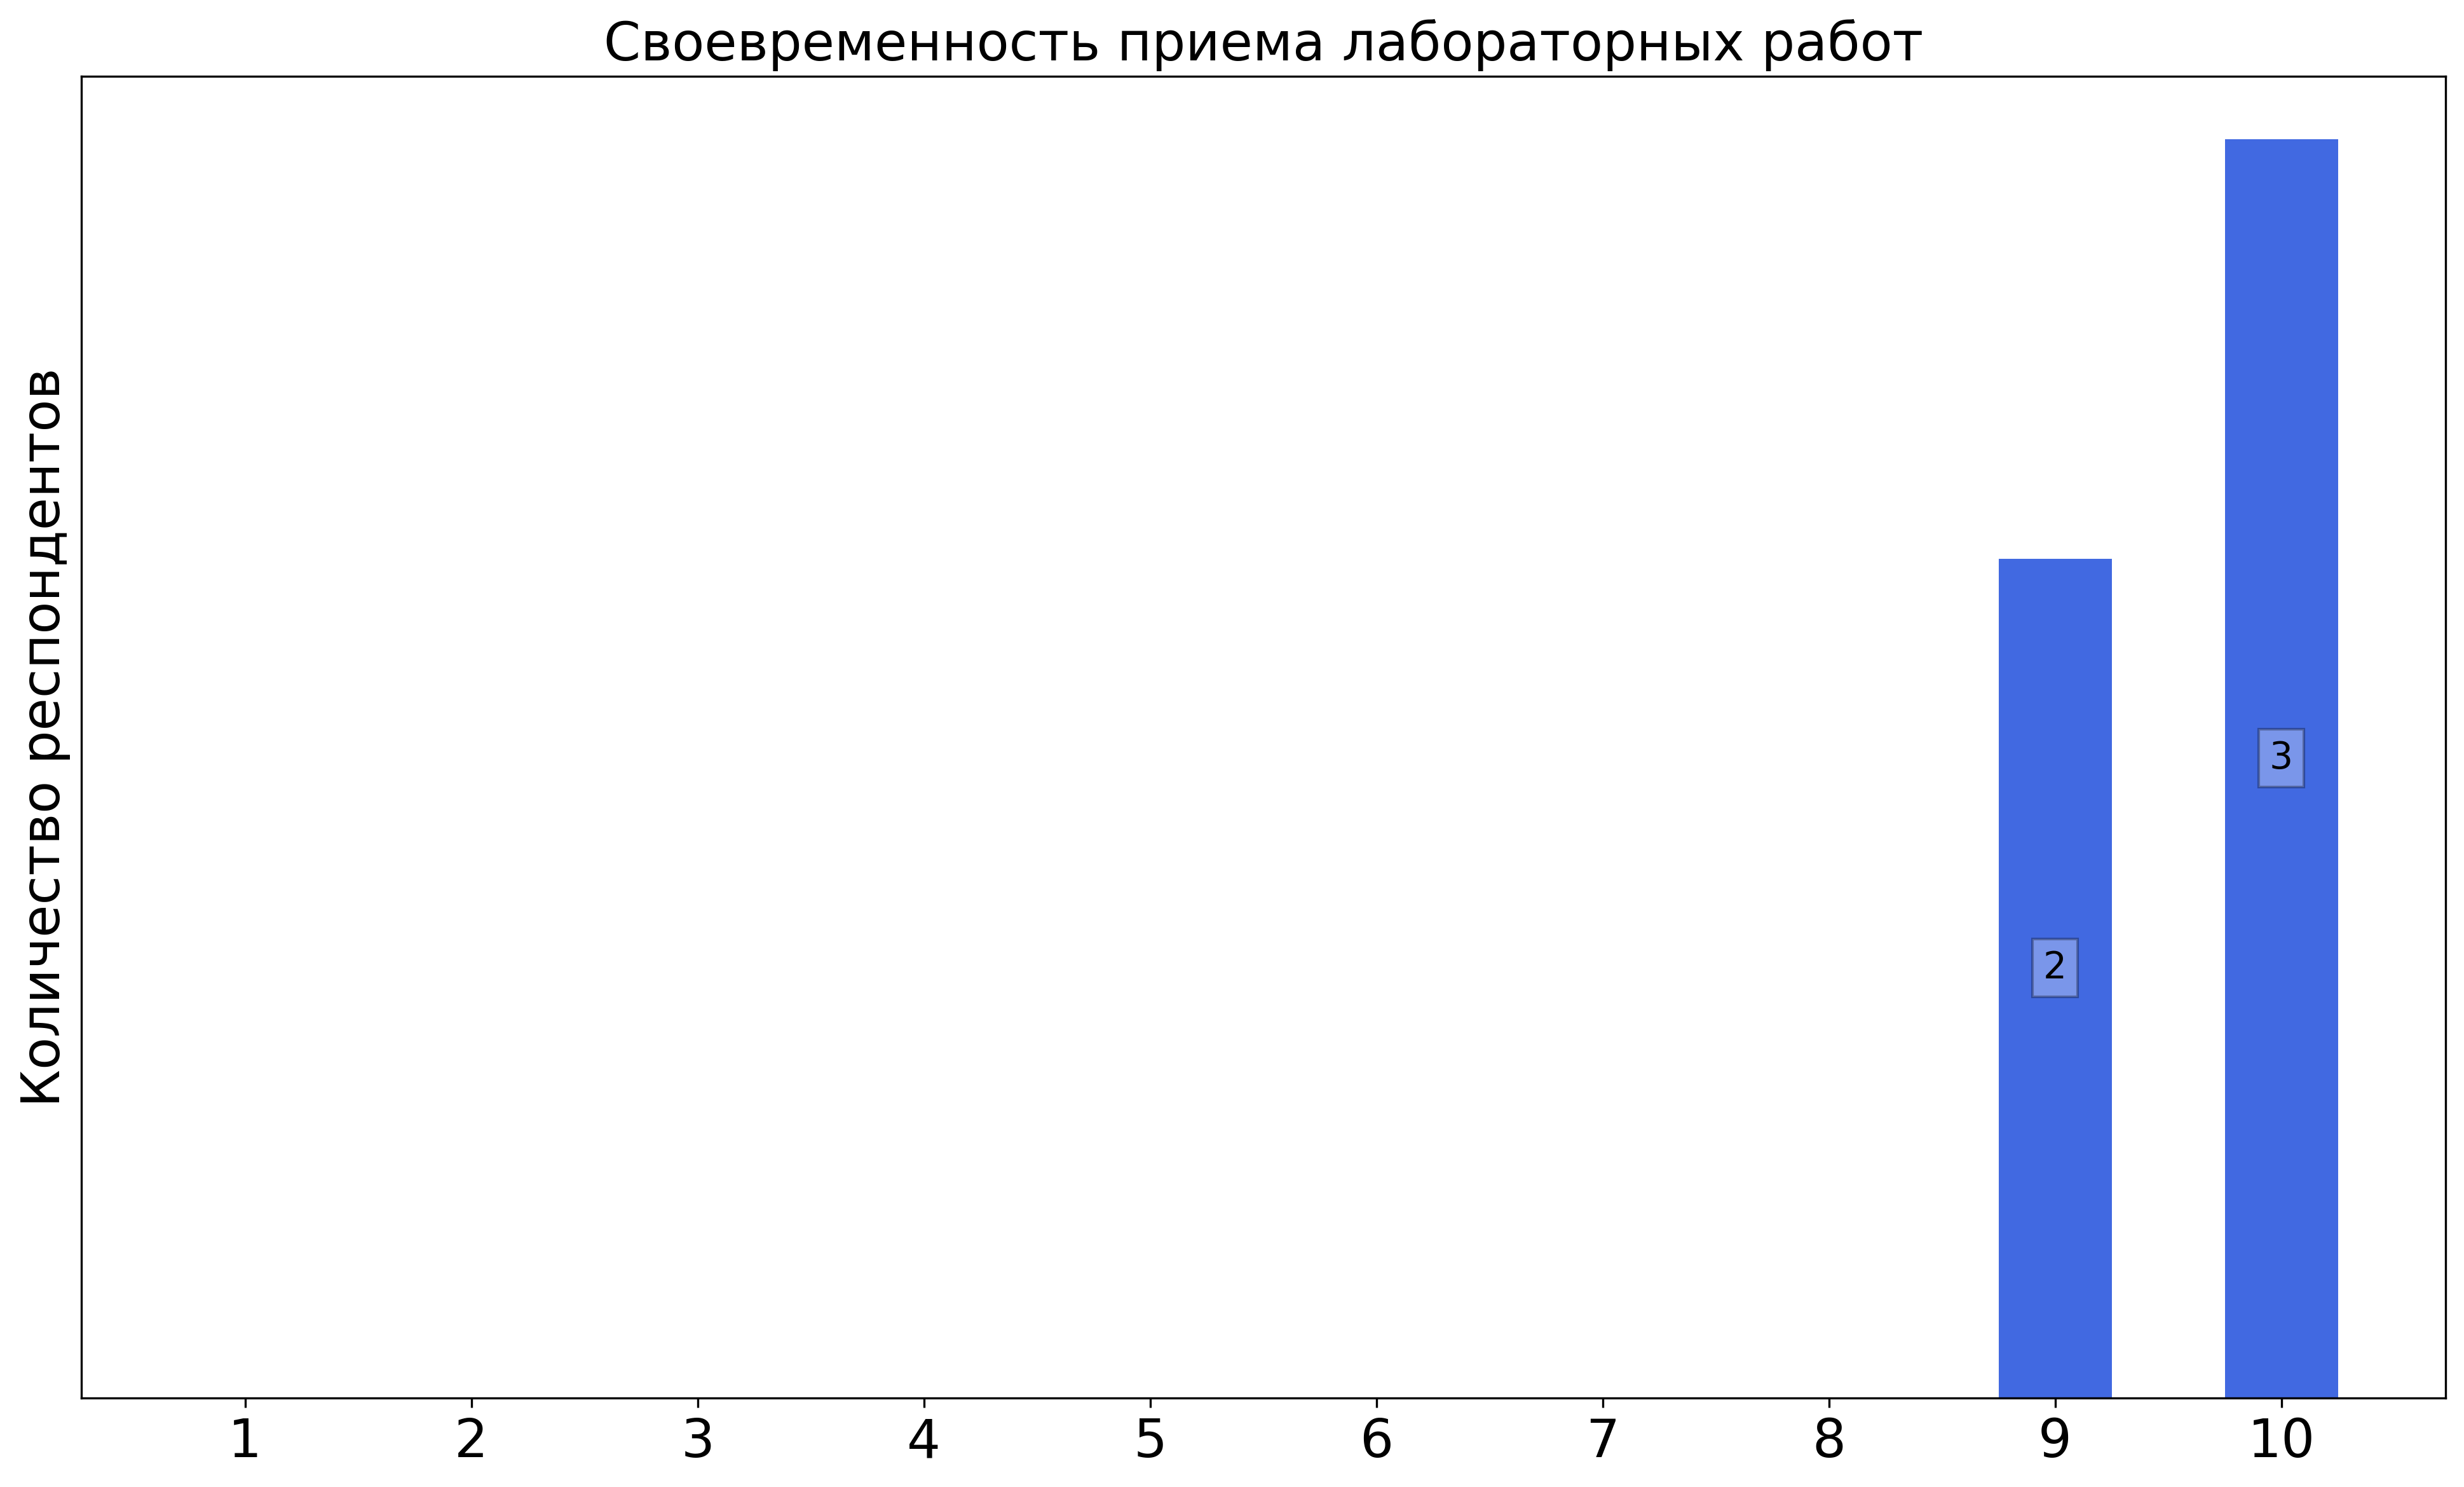
\includegraphics[width=\textwidth]{images/3 course/Аналоговая электроника/labniks-marks-Тужилкин В.А.-2.png}
			\end{subfigure}
			\begin{subfigure}[b]{0.45\textwidth}
				\centering
				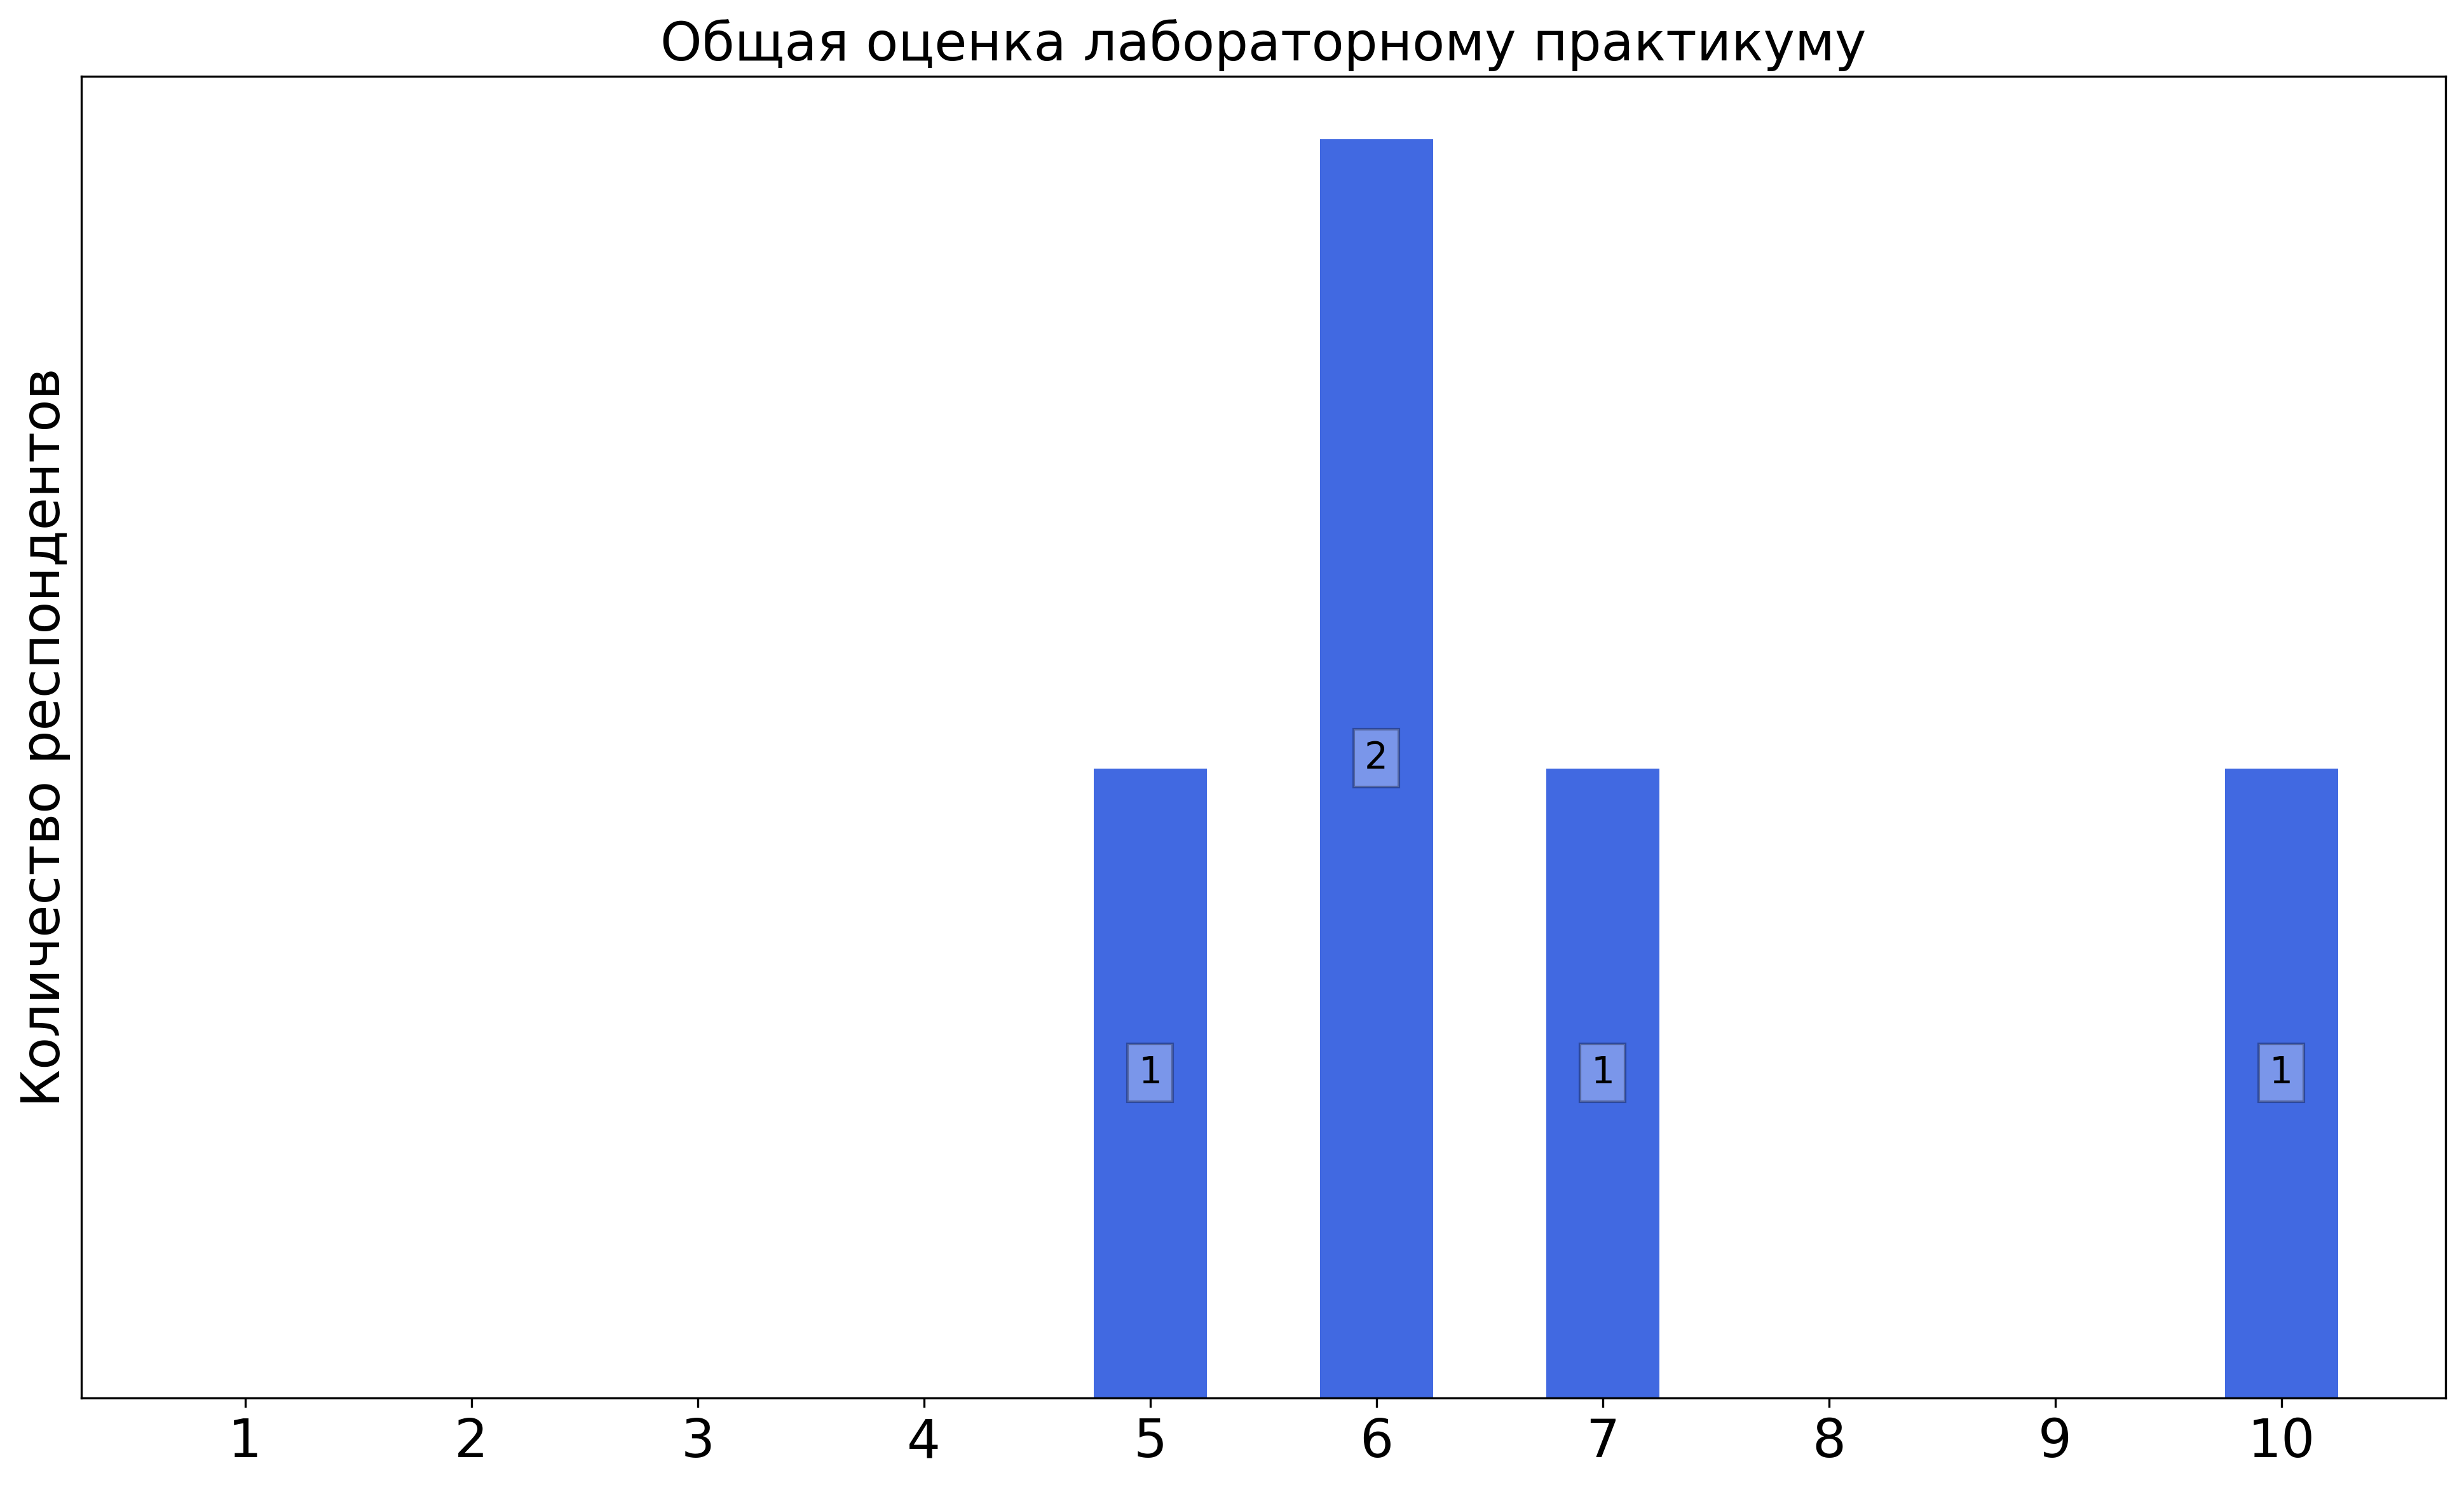
\includegraphics[width=\textwidth]{images/3 course/Аналоговая электроника/labniks-marks-Тужилкин В.А.-3.png}
			\end{subfigure}	
			\caption{Оценки респондентов о качестве преподавания лабораторных работ}
		\end{figure}

		\textbf{Комментарии студентов о преподавателе\protect\footnote{сохранены оригинальные орфография и пунктуация}}
            \begin{commentbox} 
                Перегружен по объему материала, никто нормально не зашарил 
            \end{commentbox} 

            \begin{commentbox} 
                Устаревшее оборудование, которое работает через раз. Непонятные методички. Старался читать теорию по Ларину, но это очень труднозатратно. В общем и целом, курс прошел мимо меня. 
            \end{commentbox} 

            \begin{commentbox} 
                Мне это ничего не дало, лично мне 
            \end{commentbox} 


    \subsubsection{Отзыв студентов о лабораторных работах. Преподаватель: Шабалина А.С.}
		\begin{figure}[H]
			\centering
			\begin{subfigure}[b]{0.45\textwidth}
				\centering
				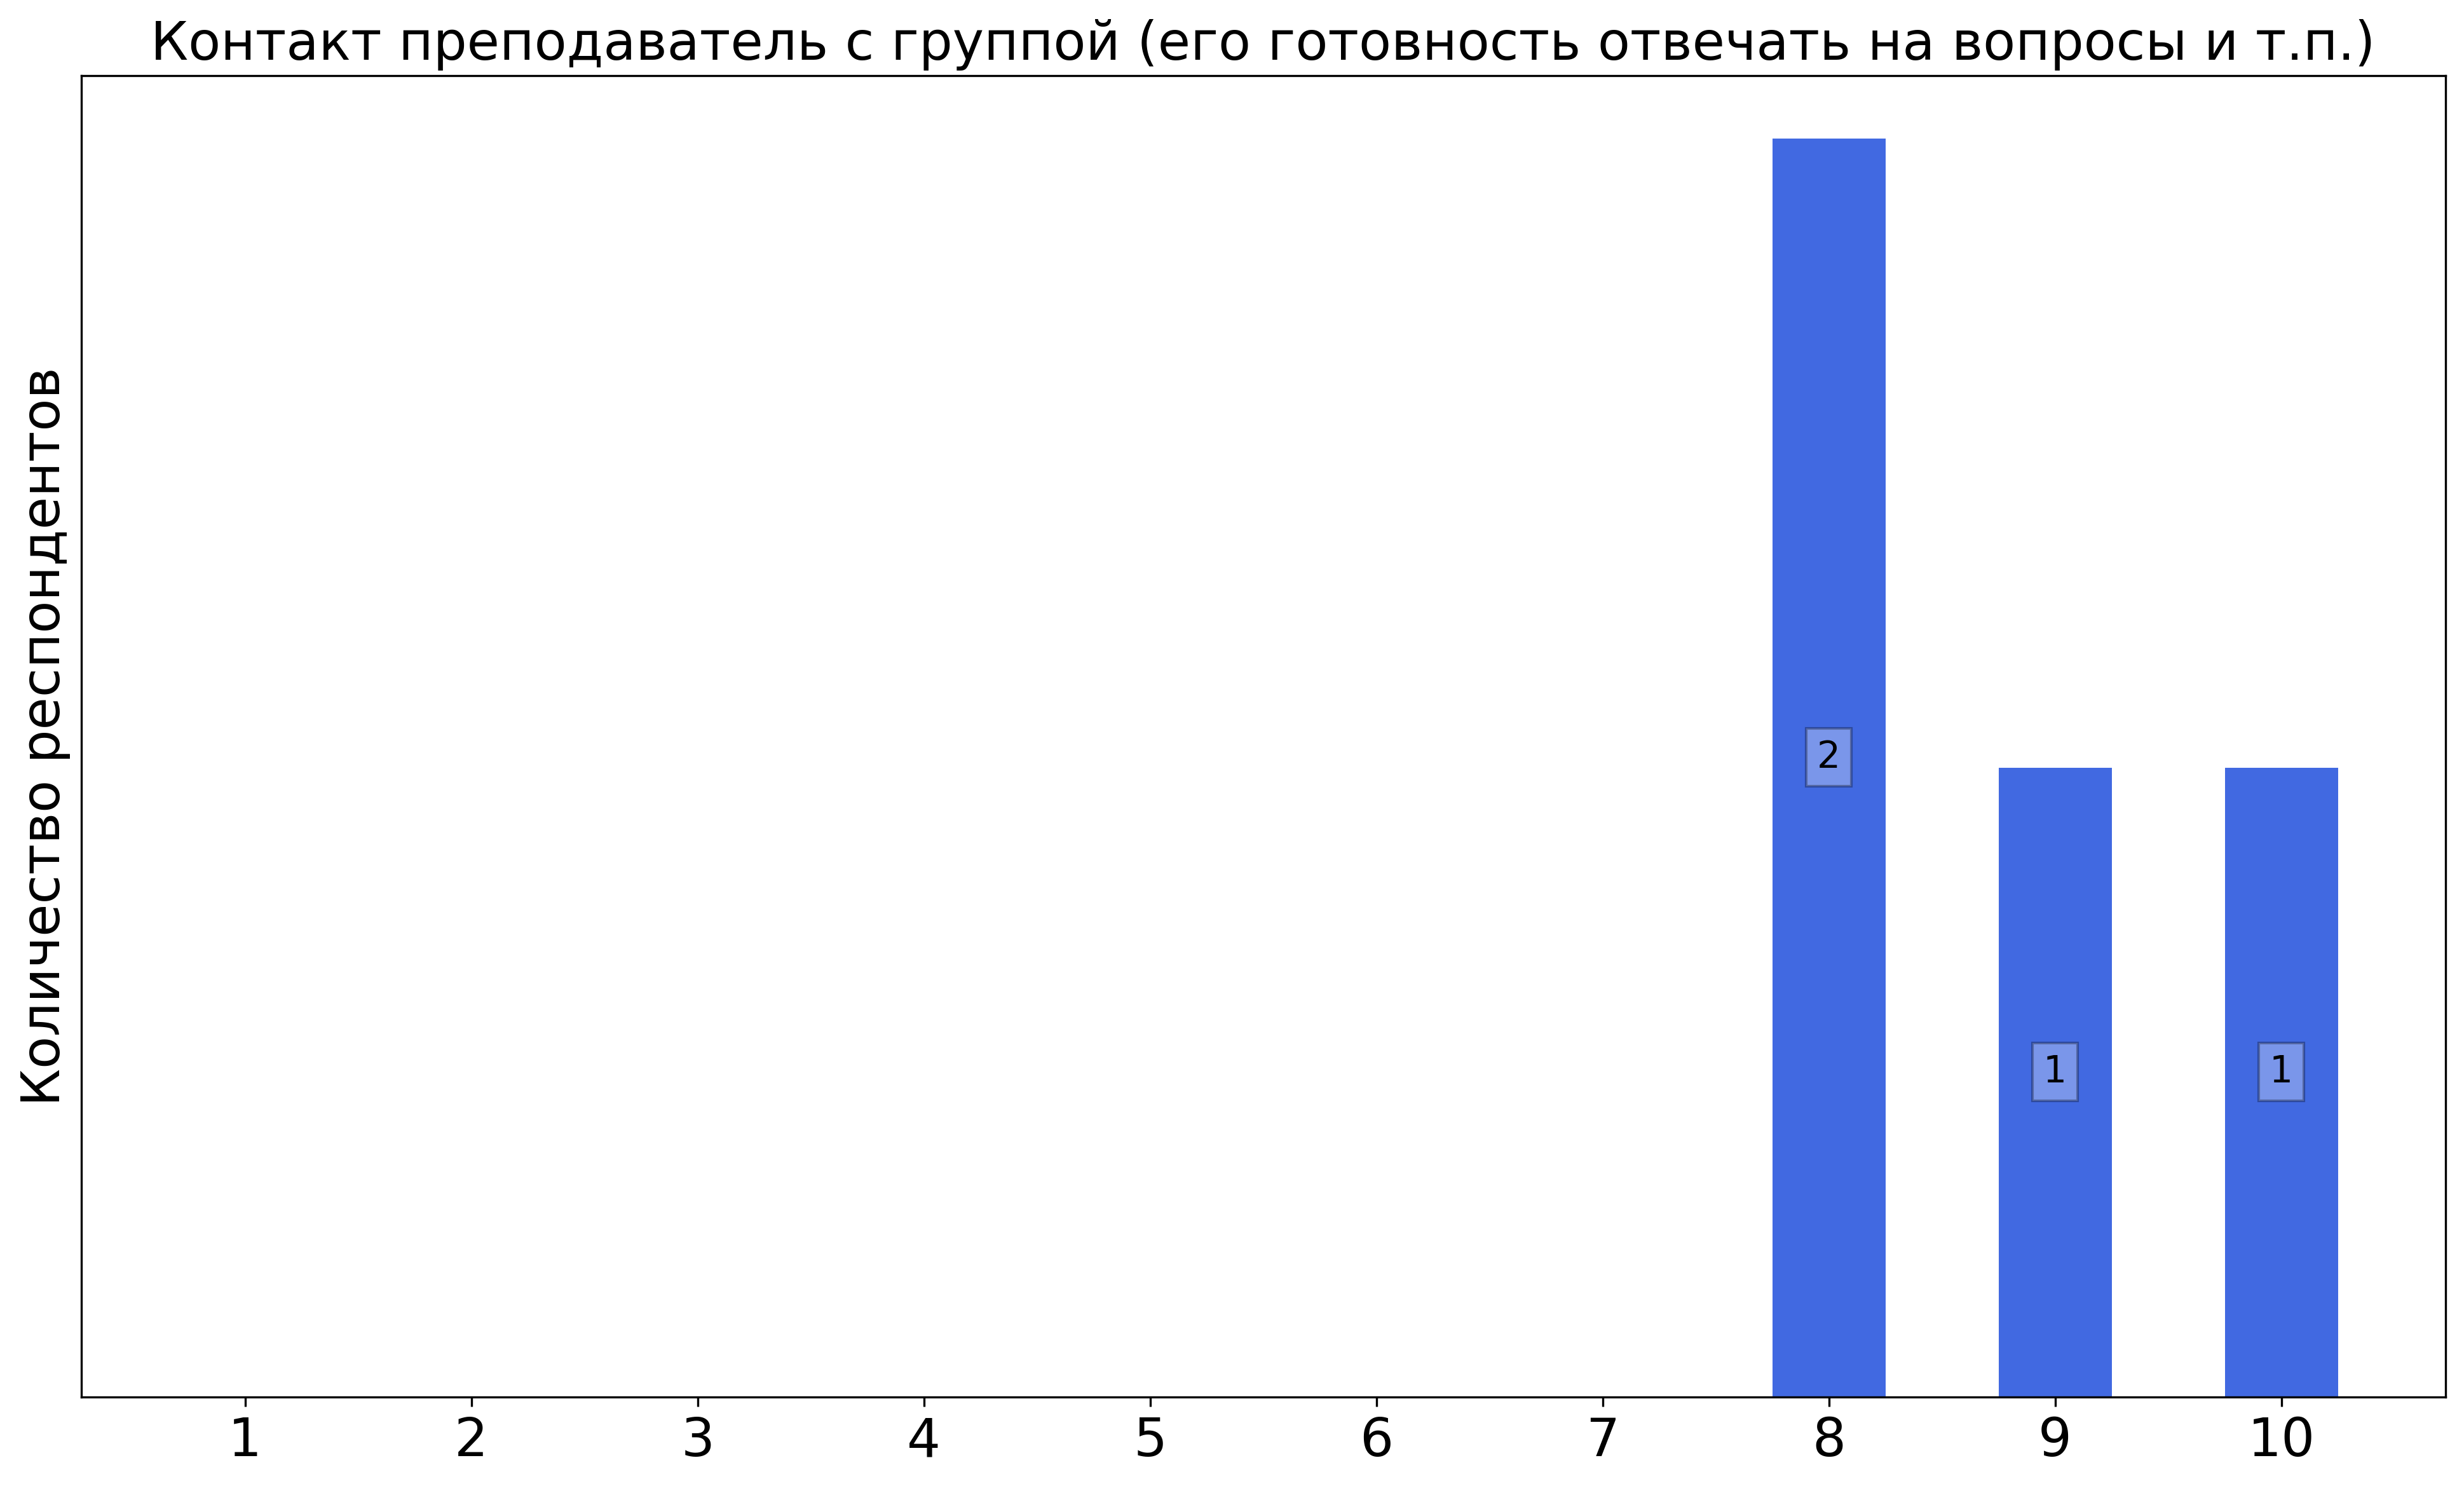
\includegraphics[width=\textwidth]{images/3 course/Аналоговая электроника/labniks-marks-Шабалина А.С.-0.png}
			\end{subfigure}
			\begin{subfigure}[b]{0.45\textwidth}
				\centering
				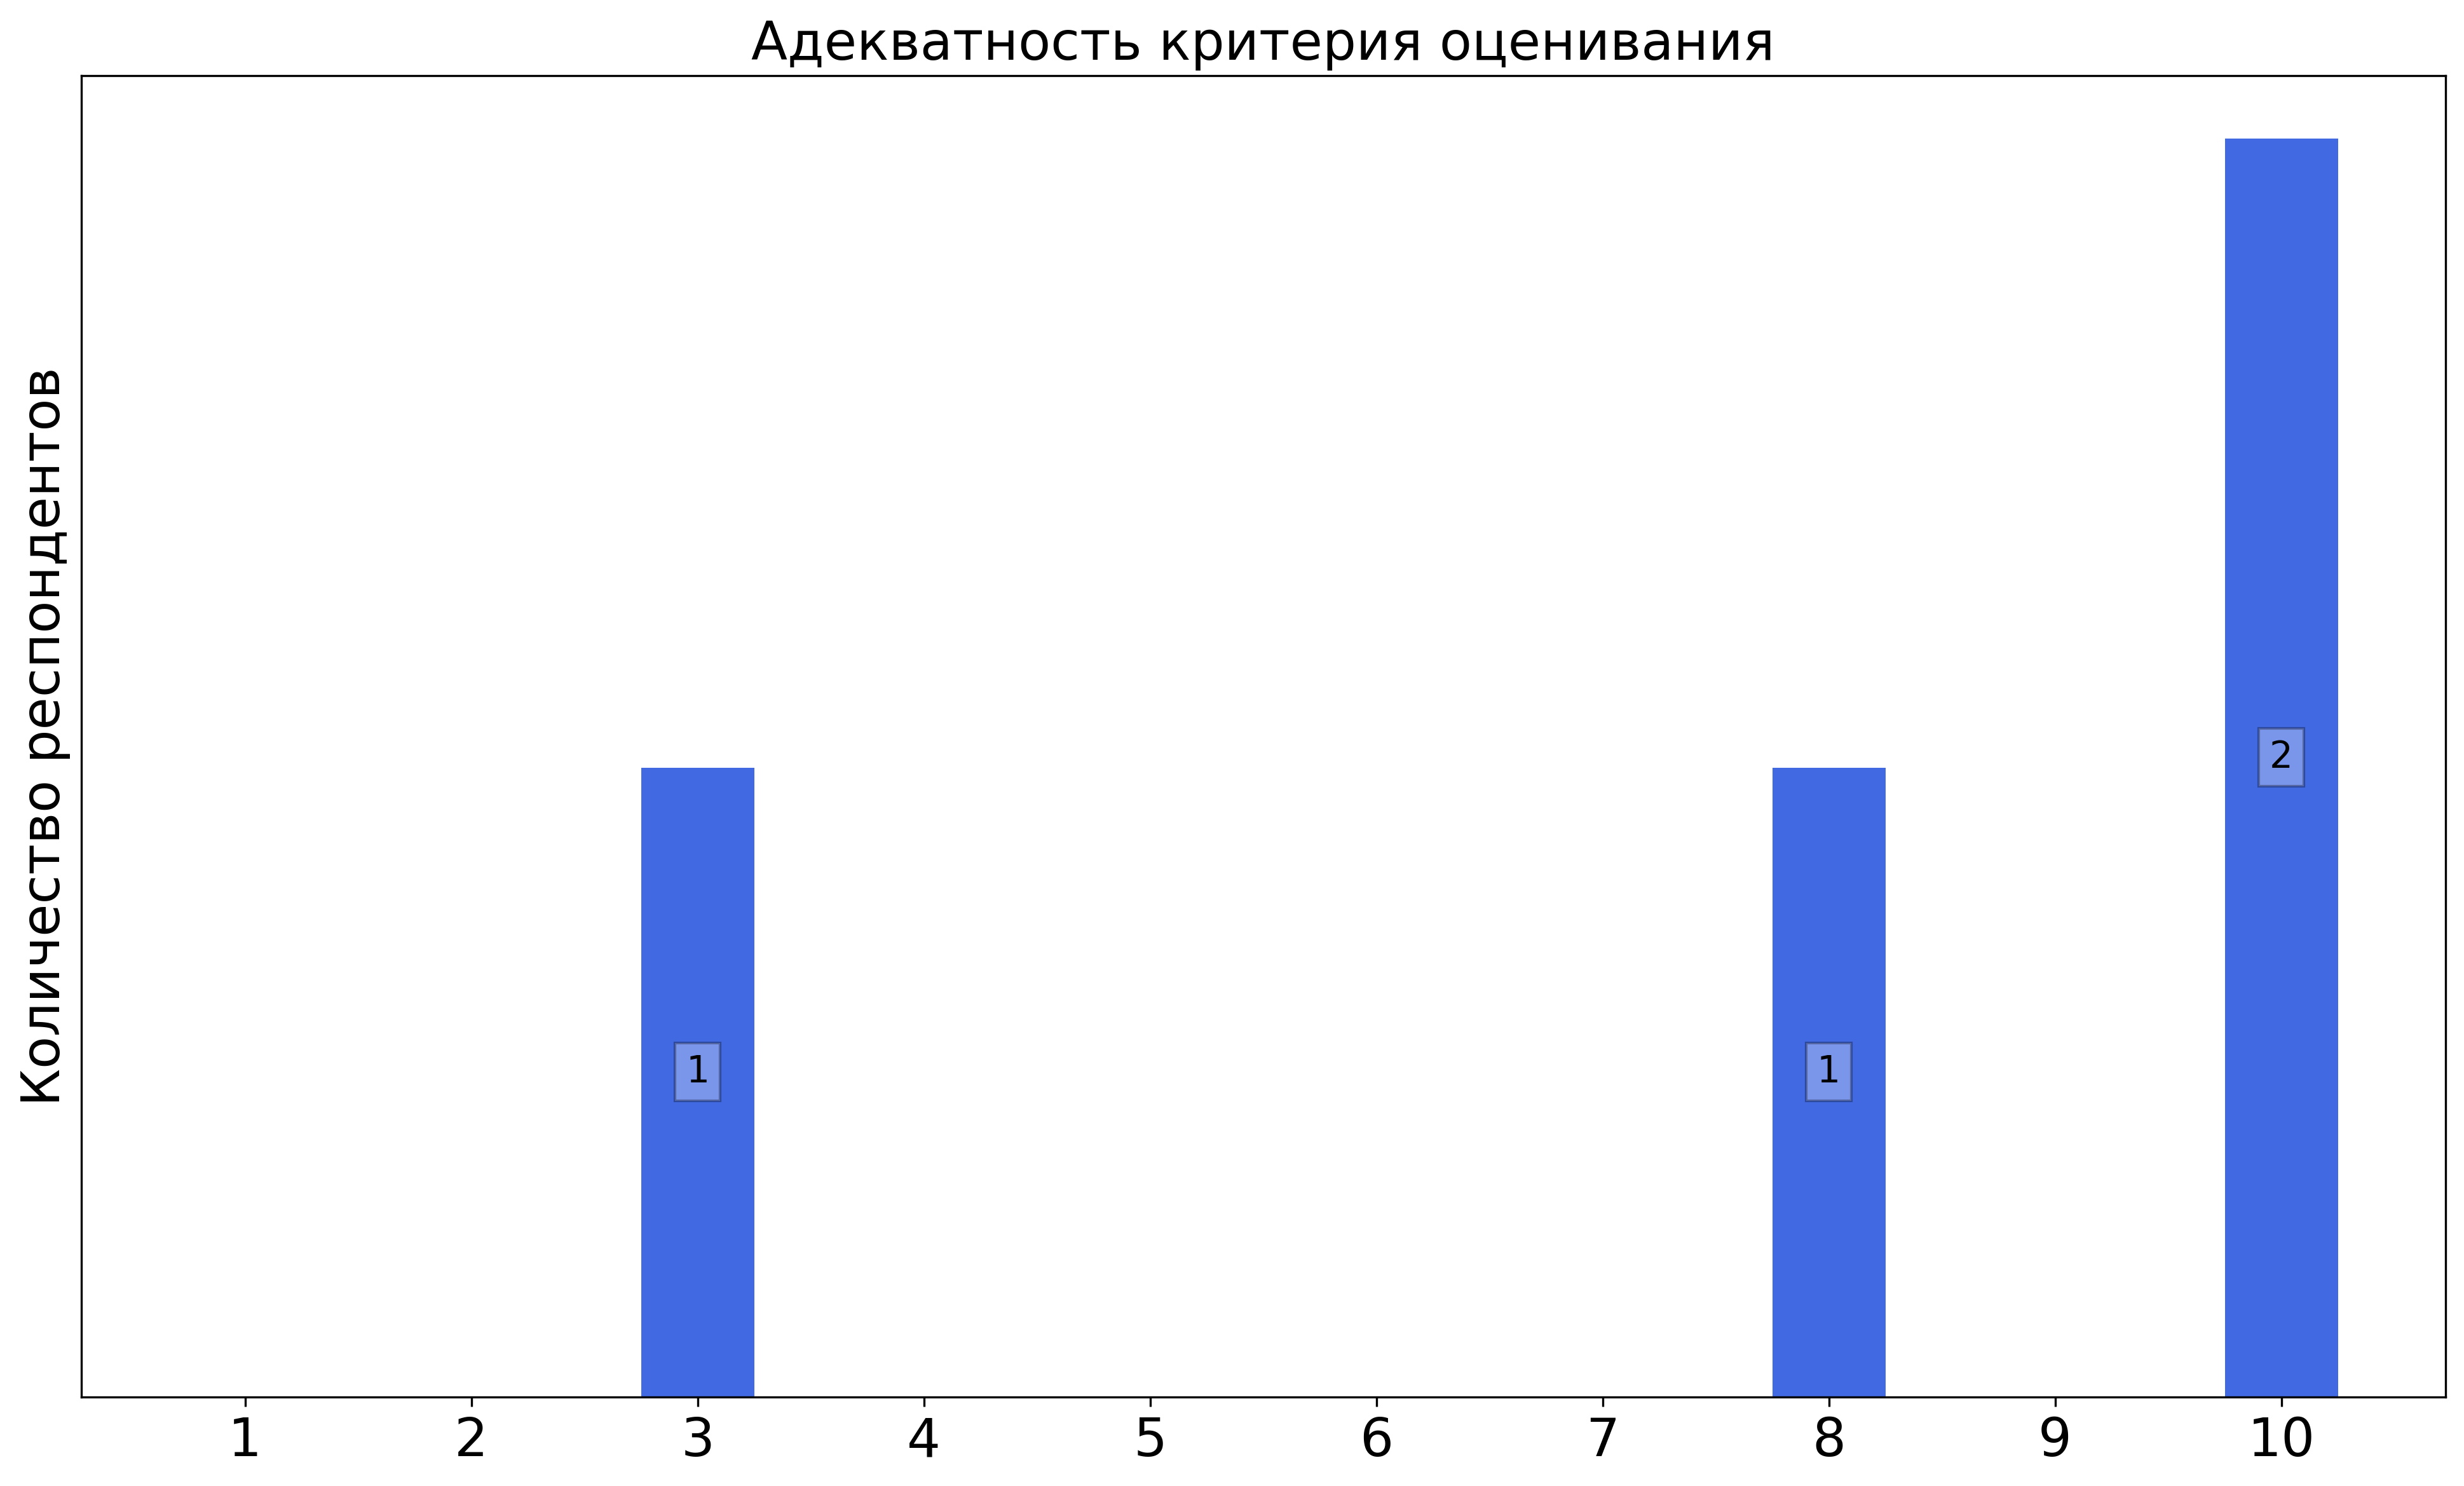
\includegraphics[width=\textwidth]{images/3 course/Аналоговая электроника/labniks-marks-Шабалина А.С.-1.png}
			\end{subfigure}
			\begin{subfigure}[b]{0.45\textwidth}
				\centering
				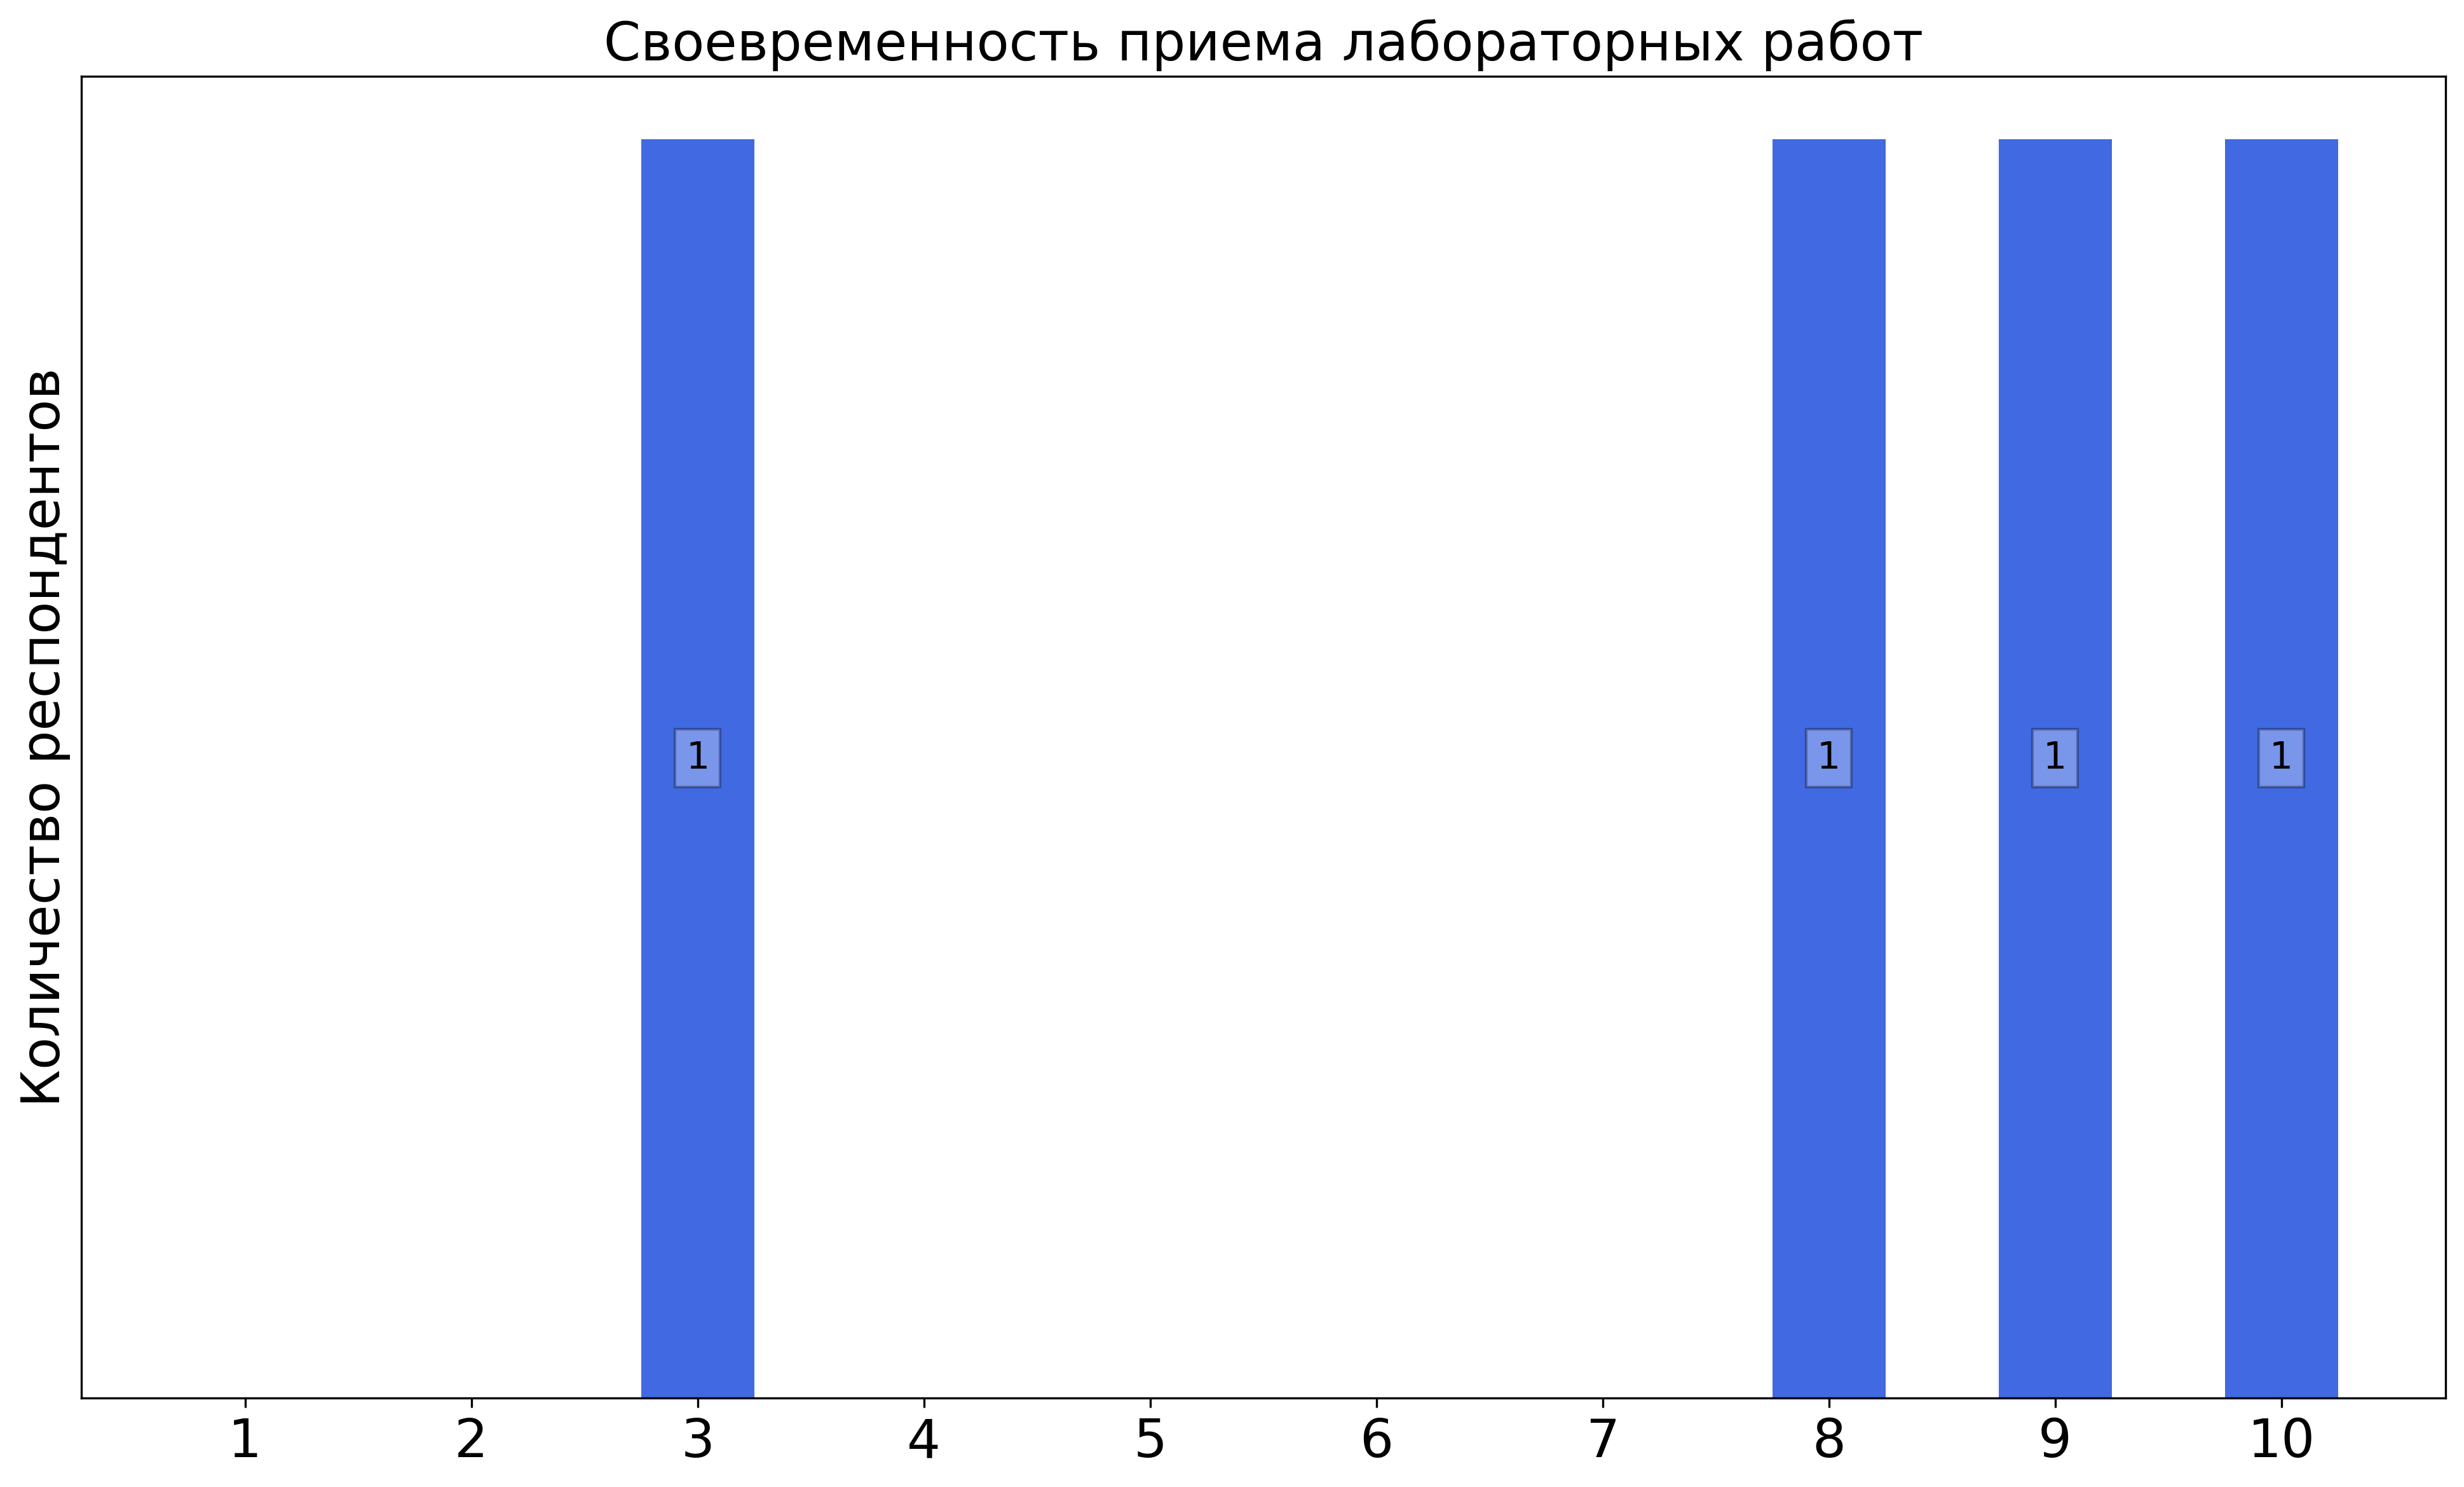
\includegraphics[width=\textwidth]{images/3 course/Аналоговая электроника/labniks-marks-Шабалина А.С.-2.png}
			\end{subfigure}
			\begin{subfigure}[b]{0.45\textwidth}
				\centering
				\includegraphics[width=\textwidth]{images/3 course/Аналоговая электроника/labniks-marks-Шабалина А.С.-3.png}
			\end{subfigure}	
			\caption{Оценки респондентов о качестве преподавания лабораторных работ}
		\end{figure}

		\textbf{Комментарии студентов о преподавателе\protect\footnote{сохранены оригинальные орфография и пунктуация}}
            \begin{commentbox} 
                Анна Сергеевна отличный лабник! 
            \end{commentbox} 
        
            \begin{commentbox} 
                Абсолютно адекватные критерии оценивания лабораторных работ, хорошие объяснения теории перед выполнением, конструктивные ответы на вопросы 
            \end{commentbox} 
        
            \begin{commentbox} 
                Неадекватные критерии оценивания. Для получения минимальной оценки (уд 3) недостаточно продемонстрировать знание теории и понимание лабораторной. Семинарист требует дотошного выполнения всех пунктов, много времени уходит, чтобы разобраться с оборудованием 
            \end{commentbox} 
        
            \begin{commentbox} 
                На все вопросы были получены ответы. Если не работал осциллограф или схема неверно собрана - преподаватель всегда приходил на помощь. Всем пониманием данного предмета, которое у меня сложилось, я обязана Анне Сергеевне 
            \end{commentbox}

    
    \subsubsection{Прочие комментарии и предложения по улучшению курса}
		\begin{commentbox}
			Убрать экзамен по РТ-цепям. Какая-то формальность, как для студентов, так и для преподавателей, о чем говорит то, что они на экзамен появляются через 2-3 часа после начала экзамена, а студенты сидят в аудитории по 4 часа, потому что принимать это все дело некому толком. Экзамен нужен только лишь для того, чтобы студенты не поехали пораньше домой. Во время сдачи лабораторных материал усваивается достаточно хорошо. Да и как можно проводить экзамен по предмету, где лектор по сути сам не понимает, что читает с листочка
		\end{commentbox}

        \begin{commentbox}
            Сделать его курсом по выбору
        \end{commentbox}

        
        \begin{commentbox}
            Уберите Дунаеву, пожалуйста
        \end{commentbox}

        
        \begin{commentbox}
            Поменять лектора!
        \end{commentbox}

        
        \begin{commentbox}
            Обновить оборудование, методички. Сделать сборник задач, чтобы можно было понять и закрепить теорию. Как один из вариантов, сделать проектный курс по аналоговой электронике наподобие проектному курсу лаб. работ по общей физике.
        \end{commentbox}

        
        \begin{commentbox}
            Поставить лектора получше, сделать методички понятнее и без лишней инфы
        \end{commentbox}

        
        \begin{commentbox}
            "Очные лекции прошли зря, лектор пока не в состоянии хорошо донести материал курса, потому что предмет выходит за рамки четырехэтажных формул, а без связанного повествования на ""качественном"" уровне выписывание формул теряет всякий смысл. Требование писать тесты по лекции и формат лабораторных работ требуют заучивания формул, оставляя значительно меньшее время на просмотр полезных лекций, которые доносят суть всех выкладок. При этом на экзамене идет спрос качественного понимания и по всей программе.

            Программу по предмету по моему реально подвергнуть корректировкам без больших затрат(лекции на основе лекций Григорьева), что значительно улучшит все возможные метрики качества(с учетом очевидных прикладных критериев к предмету)"
        \end{commentbox}

        
        \begin{commentbox}
            Заменить старое оборудование, и сделать что-то с не работающими материалами для ЛР. В целом наполнение курса интересное, на как будто немного устарело и для того чтобы заботать этот семестр совершенно не нужно знать предыдущие 2(в предыдущие года я не ботал этот предмет, а в этом получил 10 за лабы). Вообщем было бы круто как-то ужать 3 семестра аналоговой электроники и добавить больше цифры и архитектуры.
        \end{commentbox}

        
        \begin{commentbox}
            "Аналогично предлагаю поднимать интерес к электронике - очень грустно видеть, что экзамен по ней вызывает у всех смех, а не какое-либо волнение или интерес.

            !!! Например, считаю необходимым добавить в учебный план хотя бы 1 час в неделю на СЕМИНАРЫ по радиотехническим предметам (с 3 по 6 семестр), поскольку на лабораторных у многих не хватает времени отработать решение задач, да этого и не должно быть на лабораторных, а умение их решать, например, нужно на экзамене и, тем более, в жизни!!!"
        \end{commentbox}
        
        \begin{commentbox}
            Хотелось бы чтобы кто-то кроме Григорьева понятно читал этот предмет.  Грустно, что лучший лектор по рт-предметам читает этот курс у других факультетов, а не у главных ртшников физтеха (собственно, у ФРКТ). Также надеемся, что на Физтехе появятся другие реально шарящие в рт-цепях и умеющие читать их люди, готовые полностью отдаваться вузу (от некоторых крутых препов слышал, что они тянут нагрузку только как лабники)
        \end{commentbox}

        \begin{commentbox}
            Необходимо  сменить лектора и модифицировать методички для лабораторных работ
        \end{commentbox}

        \begin{commentbox}
			Я считаю, что нужно внести больше элементов семинары, а не лабораторной работы, мне было бы интереснее научиться считать все эти схемы, а не сразу пытаться делать это на сдачах или экзамене. + Было бы разумно делать Лабы менее содержательными и тогда уже по ним более детально спрашивать. это было бы эффективноее
		\end{commentbox}

        \begin{commentbox}
			"Честно, я бы очень хотел разбираться в современной инженерии, уметь делать что-то в кибернетике. Заниматься актуальными вещами.

            Но сейчас я ненавижу радиотехнику, я ненавижу то, что она у меня есть в программе, я ненавижу эту кафедру, меня раздражает её бесполезность и устаревшесть того, что я изучаю. Ужасные лекторы, неинтересные темы, отсутствие нормальной литературы, отсутствие нормальных курсов, пожилой преподавательский состав, что говорит о том, что то, что мы изучаем, никому в современном мире не нужно. 

            Пожалуйста, я очень прошу, измените эту ситуацию, сделайте этот предмет интересным и актуальным.  Посмотрите, как его изучают в зарубежных вузах, сделайте его проектным. Там же просто кучу всего можно делать. И сделать интересно, современно, актуально.

            Мы живём в эпоху, когда роботы будут активно создаваться. Так давайте вместе со всем миром этим заниматься. Я знаю, что в Сбере занимаются роботами и чем-то таким с железяками. 

            Вы же понимаете, что на РТ не хотят многие поступать или уходят отсюда как раз из-за убогого курса радиотехники и всех профильных для РТ предметов? Буквально, всё, что связано с предметами РТ - это ужасные и бесполезные курсы. Они раздражают большую часть студентов. И большая часть никто в жизни больше подобных тем касаться не хочет. И это заслуга факультета радиотехники, который разочаровывает почти всех, кто пришёл сюда за радиотехникой/инженерией/электроникой и подобным."
		\end{commentbox}

        \begin{commentbox}
			"Избавиться от формализма

            Придумать универсальный дебильник для закрытия зачёта и экзамена. Чтобы каждый студент, который пропустил какие-то пары/лекции мог подготовиться к письменному экзамену и одновременно закрыть оба зачёта. 
            Короче, хочется чтобы критерии оценивания соответствовали ожиданиям кафедры от студентов. А так получается, что кафедра требует от студента вкладывать уйму времени, читать плохие методички и вникать в устаревшее оборудование, а сама устаивает абсолютно формальный экзамен, где от качества подготовки ничего не зависит. "
		\end{commentbox}

        \begin{commentbox}
			Поменять лектора, возможно пересмотреть подход к изучению предмета, потому что такое ощущение, что всем студентам на предмет все равно. 
		\end{commentbox}

        \begin{commentbox}
			Большая просьба поставить читать лекции на ФРКТ на старших курсах А.А. Григорьева (или человека вроде него), поскольку в противном случае РТшники так и будут так себе знать свой профильный предмет. Проблема в том, что на 3+ курсе для того, чтобы заинтересовать студентов (которые уже хотят только работать), нужен лектор вроде Григорьева: человек с харизмой и умением просто рассказывать сложное. Монотонное же зачитывание материала без особых пояснений не сильно этому способствует.
		\end{commentbox}

        \begin{commentbox}
			Качество материалов отвратительное - лекции слушать бесполезно, единственный хороший лектор - Григорьев, его очень интересно слушать, а объяснения понятные, но его лекции для ФАКТа не охватывают весь курс аналоговой электроники, к сожалению. Многие отмечали, что им нравятся лекции Ларина и его книжка - мне не становилось понятнее, возможно, дело во мне. Методички по лабам, как всегда, ужасны и абсолютно нечитаемы. Всё, что было понято мной в рамках курса, было вынесено из некоторых лекций Григорьева, несмотря на мои многочисленные попытки лучше и усерднее подготовиться к лабам
		\end{commentbox}

        \begin{commentbox}
			Само по себе наличие курса аналоговой электроники в современных реалиях ФРКТ вызывает огромные вопросы. На мой взгляд, уместнее было бы ограничиться двумя первыми семестрами РТ-лаб, а впоследствии перейти сразу к цифровой электронике, сделав её обязательной только для студентов кафедр, связанных с ней. Лектор по курсу ужасен, не понятно ничего, а наличие экзамена по абсолютно бесполезному курсу и вовсе абсурдно. Наверное, если бы лекции читал Григорьев А. А. или какой-нибудь другой преподаватель кафедры, интересно преподносящий материал (к примеру, Григорьев И. А. или Неешпапа А. В.), взгляд на курс мог бы быть иным, но в нынешнем исполнении о нём нельзя сказать ни единого хорошего слова. Предмет бесполезен, на лекциях ничего не понятно, из-за чего приходится смотреть другого лектора в записи, а курс лабораторных работ не имеет никакого прикладного применения. Вишенкой на торте является наличие экзамена по данному курсу, учитывая качество его преподавания и общую бесполезность.
		\end{commentbox}

        \begin{commentbox}
			Курс в текущем ключе видится просто бесполезным, тратится много времени на попытки понимания, а выхлоп нулевой. Лектора нужно менять. На лабораторные поискать новых молодых лабников, у которых есть понимание, что происходит в головах студентов после прочтения ужасных методичек.
		\end{commentbox}

        \begin{commentbox}
			Убрать курс или полностью переделать, иначе это бесполезная трата сил и времени студентов
		\end{commentbox}

        \begin{commentbox}
            Описал  графе с лекциями. Стоит что-то сделать тем как лектор читает лекции. Лично я расположил бы лекторов по качеству преподования материала от лучших к худшим в такой последовательности: Григорьев А.А., Ларин А.Л., Филатов И.В. , Дунаева М. А.
        \end{commentbox}
